\documentclass[a4paper, 14pt]{extarticle}
\usepackage[margin=1in]{geometry}
\usepackage{amsfonts, 
			amsmath, 
			amssymb,
			amsthm,
			pgfplots,
			tikz,
			graphicx,
			caption,
			float,
			physics
			}

\usepackage[utf8]{inputenc}
\usepackage[english, main=ukrainian]{babel}
\usepgfplotslibrary{fillbetween}
\usepackage[unicode]{hyperref}
\usepackage{enumitem}
\usepackage{pdfpages}
\usepackage{centernot}
%\usepackage{showframe}

\parindent 0ex

\newtheoremstyle{theoremdd} % name of the style to be used
  {\topsep} % measure of space to leave above the theorem. E.g.: 3pt
  {\topsep} % measure of space to leave below the theorem. E.g.: 3pt
  {\normalfont} % name of font to use in the body of the theorem
  {0pt} % measure of space to indent
  {\bfseries} % name of head font
  {} % punctuation between head and body
  { } % space after theorem head; " " = normal interword space
  {\thmname{#1}\thmnumber{ #2}\textnormal{\thmnote{ \textbf{#3}\\}}}

\theoremstyle{theoremdd}
\newtheorem{theorem}{Theorem}[subsection]
  
\theoremstyle{theoremdd}
\newtheorem{definition}[theorem]{Definition}

\theoremstyle{theoremdd}
\newtheorem{samedef}[theorem]{Definition}

\theoremstyle{theoremdd}
\newtheorem{example}[theorem]{Example}

\theoremstyle{theoremdd}
\newtheorem{proposition}[theorem]{Proposition}

\theoremstyle{theoremdd}
\newtheorem{remark}[theorem]{Remark}

\theoremstyle{theoremdd}
\newtheorem{lemma}[theorem]{Lemma}

\theoremstyle{theoremdd}
\newtheorem{corollary}[theorem]{Corollary}

\def\qed{$\blacksquare$}
\def\rightproof{$\boxed{\Rightarrow}$ }
\def\leftproof{$\boxed{\Leftarrow}$ }

\makeatletter
\renewenvironment{proof}[1][Proof.\\]{\par
\pushQED{\hfill \qed}%
\normalfont \topsep6\p@\@plus6\p@\relax
\trivlist
\item\relax
{\bfseries
#1\@addpunct{.}}\hspace\labelsep\ignorespaces
}{%
\popQED\endtrivlist\@endpefalse
}
\makeatother

\DeclareMathOperator{\lcm}{lcm}
\DeclareMathOperator{\ord}{ord}
\DeclareMathOperator{\ind}{ind}

\newcommand\thref[1]{\textbf{Th.~\ref{#1}}}
\newcommand\defref[1]{\textbf{Def.~\ref{#1}}}
\newcommand\exref[1]{\textbf{Ex.~\ref{#1}}}
\newcommand\prpref[1]{\textbf{Prp.~\ref{#1}}}
\newcommand\rmref[1]{\textbf{Rm.~\ref{#1}}}
\newcommand\lmref[1]{\textbf{Lm.~\ref{#1}}}
\newcommand\crlref[1]{\textbf{Crl.~\ref{#1}}}


\begin{document}
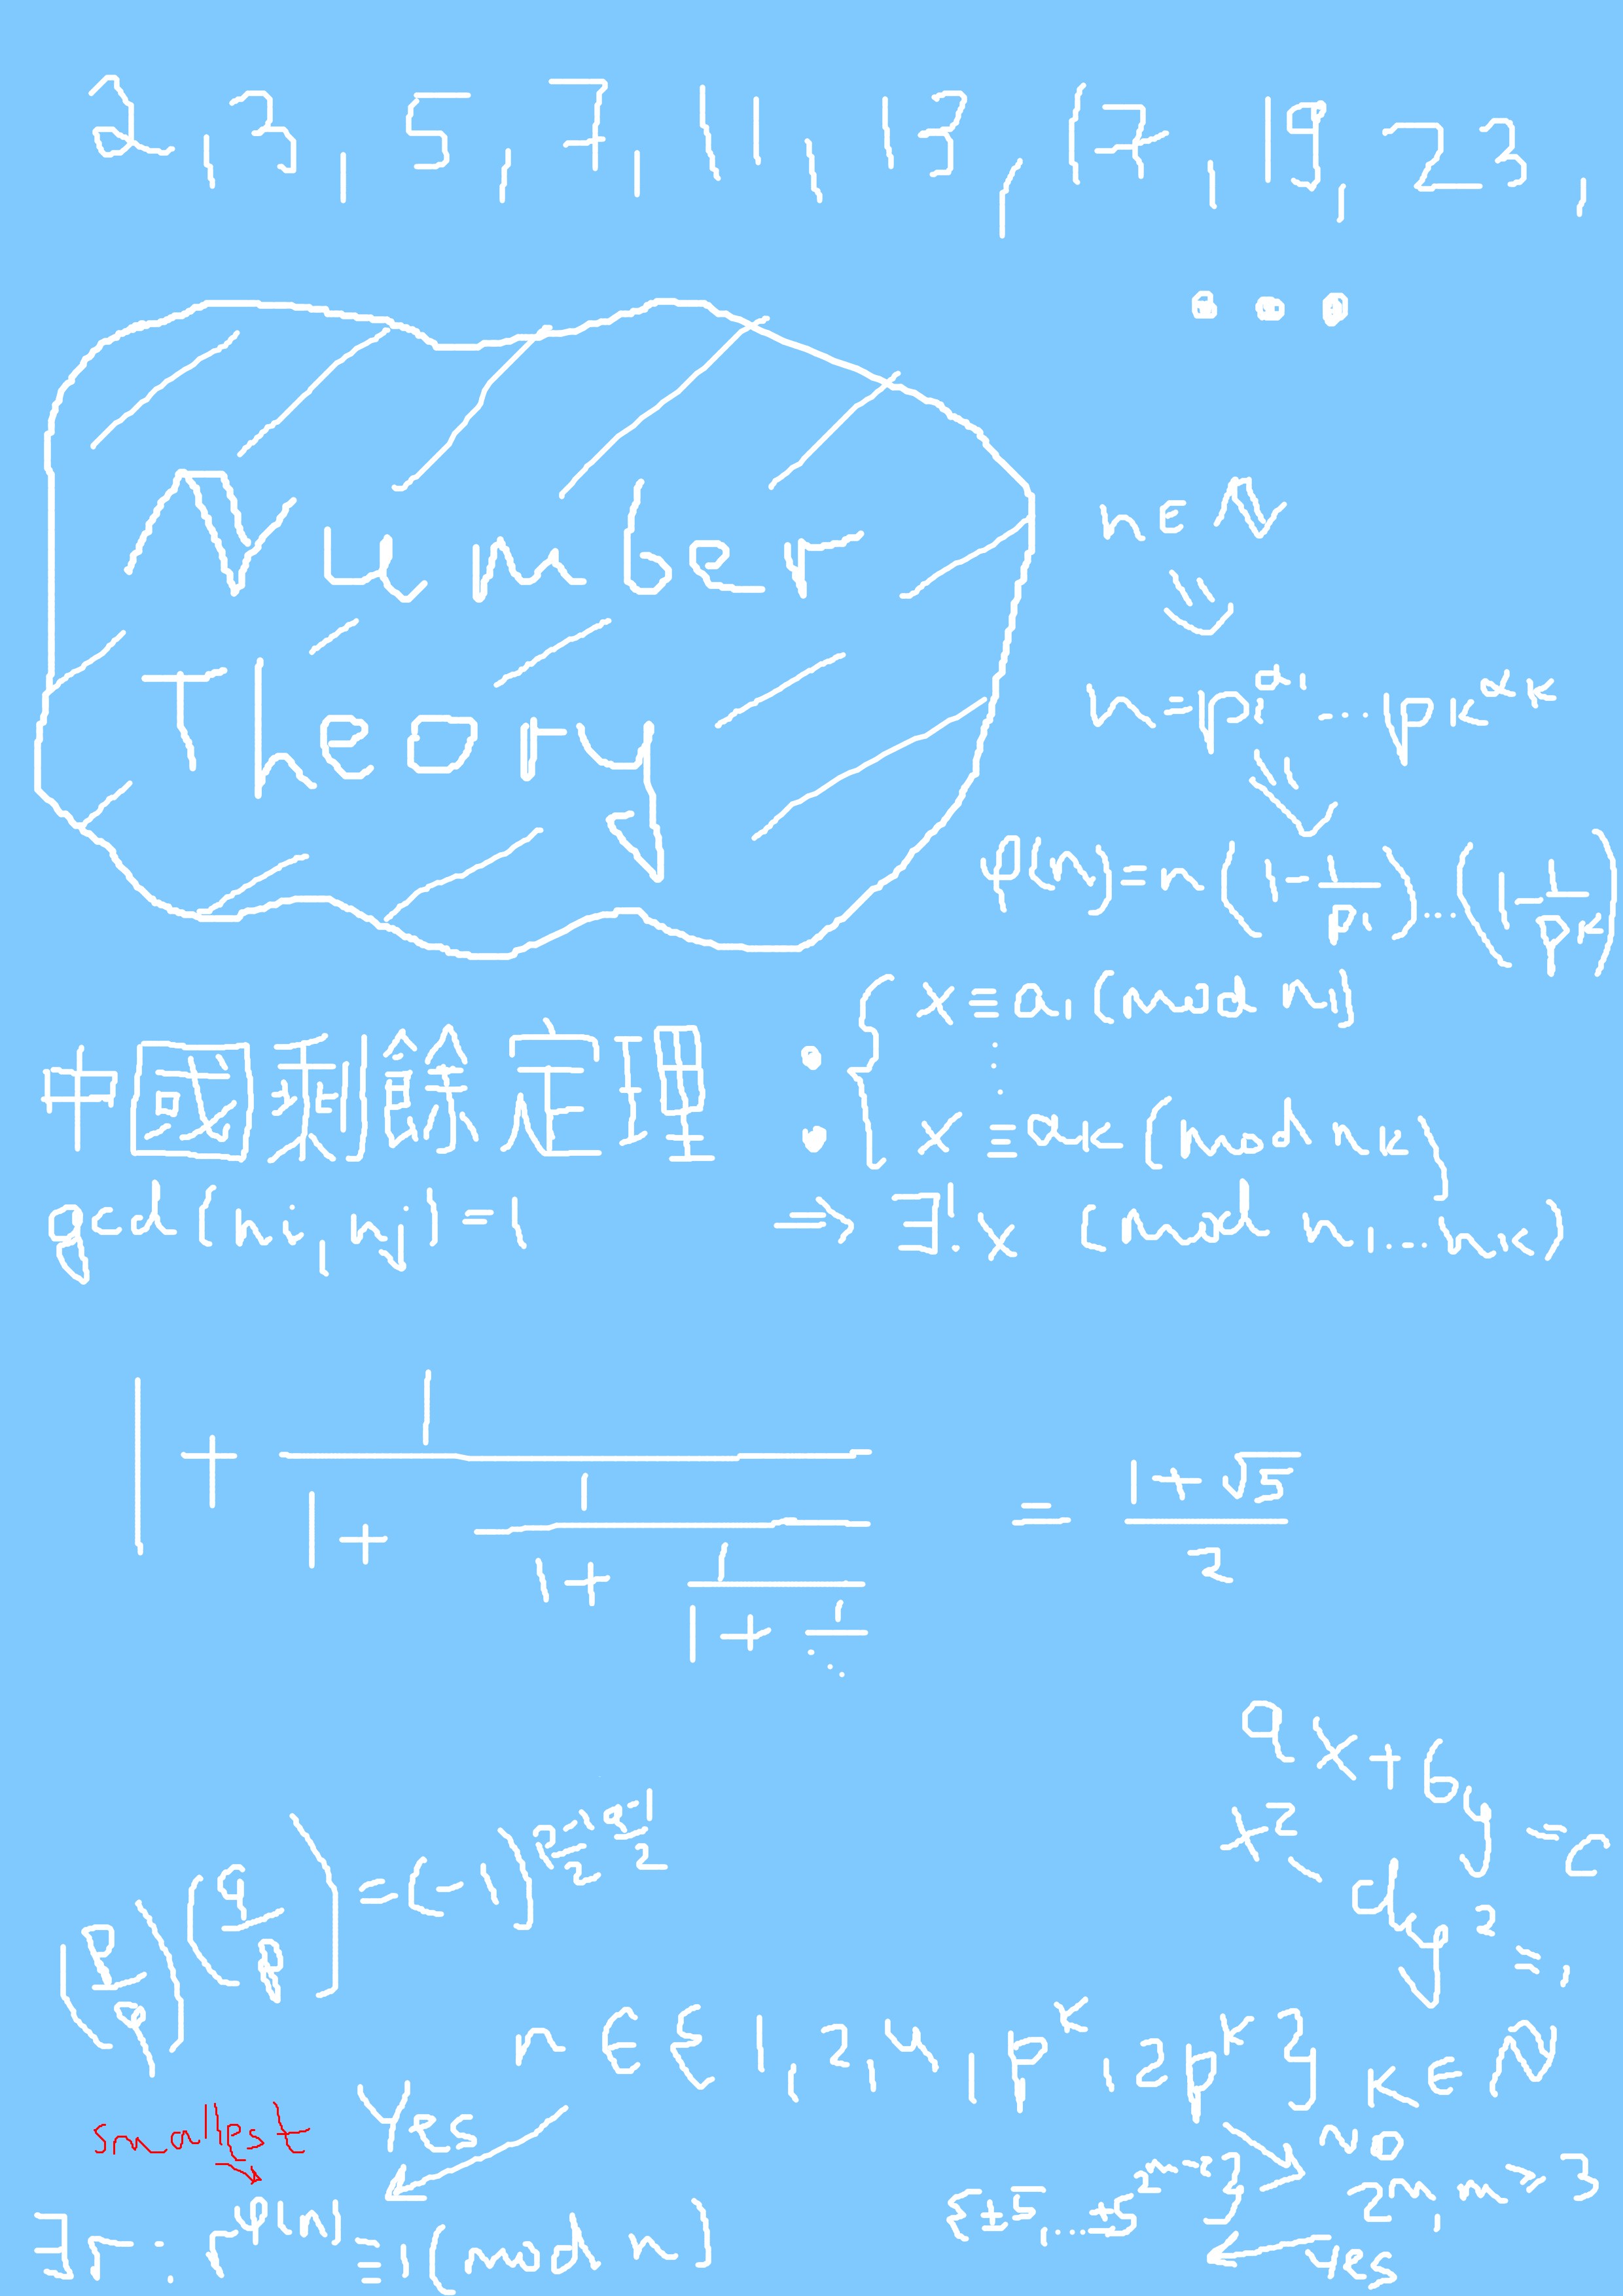
\includepdf{preview.png}
\tableofcontents
\newpage

\iffalse
\section*{Теорія чисел?}
Ну в принципі, да, але ні. Після класичної теорії чисел підуть більш комплексні теми, описуючи узагальнення теорії чисел. Спочатку пройду курс за Michael Penn з канала MathMajor, одночасно читаючи книгу Burton для повного розуміння, а далі вже узагальнення. Можливо, буду й там й там писати нові теми.
\bigskip \\
Авторські виправлення: додати Well-ordering principle, бо деякі теореми цього вимагають.
\newpage
\fi

\section{Основи теорії чисел}
\subsection{Подільність}
\begin{definition}
Задані числа $a,b \in \mathbb{Z}$, де $a \neq 0$.\\
Кажуть, що число $a$ \textbf{ділить число} $b$, якщо
\begin{align*}
\exists c \in \mathbb{Z}: b = ac
\end{align*}
Позначення: $a \mid b$.\\
Інколи кажуть, що $b$ \textbf{ділиться націло на} $a$,  позначають за $b \, \vdots \, a$.
\end{definition}

\begin{example}
Зокрема $2 \mid 6$, тому що $6 = 2 \cdot 3$.
\end{example}

\begin{remark}
$a \mid 0$, де $a$ -- будь-яке ненульове число. Справді, $0 = 0 \cdot a$.
\end{remark}

\begin{remark}
Кожне число $b \neq 0$ має скінченну кількість дільників.\\
Дійсно, візьмімо якийсь дільник $a$ числа $b$, тобто $a \mid b$, то звідси $b = ac$, а тому $|b| = |a||c| \implies |b| \geq |a|$. Остання нерівність і підтверджує слова.
\end{remark}

\begin{proposition}
Задані числа $a,b,c \in \mathbb{N}$. Тоді:
\begin{enumerate}[nosep,wide=0pt,label={\arabic*)}]
\item $a \mid a$;
\item $a \mid b$, $b \mid a \implies a = b$;
\item $b \mid a$, $c \mid b \implies c \mid a$.   
\end{enumerate}
Тобто ділення формує відношення нестрогого порядку.
\end{proposition}

\begin{proof}
Маємо таке доведення:
\begin{enumerate}[wide=0pt,label={\arabic*)}]
\item $a = 1 \cdot a \implies a \mid a$.
\item Маємо $a \mid b, b \mid a$. За означенням, існують такі числа $x,y \in \mathbb{N}$, для яких $b = ax$, $a = by$. Тоді $a = axy \implies xy = 1$. Єдиний варіант -- це одночасно $x = y = 1$. Підставляючи отримані значення, маємо $a = b$.
\item $b \mid a \implies a = bx$. $c \mid b \implies b = yc \implies a = bx = xy \cdot c \implies c \mid a$.
\end{enumerate}
Відношення порядку доведено.
\end{proof}

\begin{example}
Довести, що різниця послідовних кубів ніколи не ділиться на $2$.\\
Різниця сусідніх кубів $(a+1)^3 - a^3 = 3a^2+3a+1 = 3a(a+1)+1$. Зауважимо, що $2 \mid a(a+1)$, і дійсно:\\
якщо $a = 2k, k \in \mathbb{Z}$, то отримаємо $2 \mid 2k(2k+1)$;\\
якщо $a = 2k+1, k \in \mathbb{Z}$, то отримаємо $2 \mid (2k+1)(2k+2)$.\\
Отже, $a(a+1) = 2x$, тоді звідси $3a(a+1) = 2 \cdot (3x) = 2u$. Тобто $(a+1)^3 - a^3 = 2u+1$, а значить $2 \nmid (a+1)^3-a^3$.
\end{example}

\begin{lemma}[Ділення з остачею]
Для довільних $a,b \in \mathbb{Z}$, де число $a > 0$, існують єдині $q,r \in \mathbb{Z}$, для яких $b = qa + r$, де $r$ задовольняє нерівності $0 \leq r < a$.\\ 
Число $r$ називають \textbf{остачею} від ділення $b$ числом $a$.
\end{lemma}

\begin{proof}
I. \textit{Існування}.\\
Розглянемо множину $S = \{b - qa : q \in \mathbb{Z}\} \cap \mathbb{Z}_{\geq 0}$. Ясно, що вона непорожня, оскільки там лежить число в залежності від числа $b$:\\
або $b = b - 0 \cdot a$, якщо $b \geq 0$;\\
або $b-b \cdot a = b(1-a)$, якщо $b < 0$.\\
Також ця множина обмежена знизу, оскільки кожне число -- невід'ємне. Значить, існує $\min S$. Цей мінімум позначимо за число $r$, яке шукали.\\
Отже, $r \geq 0$, а також $\exists q \in \mathbb{Z}: r = b -qa$. Залшилося показати, що $r < a$.\\
!Якщо припустити, що $r \geq a$, то тоді $r - a \geq 0$, а число \\ $r - a = b-qa - a = b - (q+1)a \overset{q+1 = q^*}{=} b-q^*a$. \\
Таким чином, $r-a \in S$. Але ми знаємо, що $r$ -- мінімальне число цієї множини та при цьому $r - a < r$. Суперечність!
\bigskip \\
II. \textit{Єдиність}.\\
!Припустімо, що окрім $q,r$, для яких $b = qa + r$, існує ще одна інша пара $q',r'$, для яких $b = q'a + r'$. Ми тут вважаємо, що $r' < r$, для іншого випадку аналогічно. Тоді\\
$qa + r = q'a + r' \implies a(q'-q) = r - r'$. \\
Із цієї рівності випливає, що $a \mid (r-r')$. Але ми водночас маємо, що $0 < r - r' < r < a$, тоді єдиний варіант під час ділення -- це випадок $r-r' = 0 \implies r = r'$. Тоді вже звідси $q' = q$. Суперечність!
\end{proof}

\begin{example}
От уже $4 \nmid 14$, але за попередньою лемою, $4 = 3 \cdot 4 + 2$, де число $2$ -- остача.
\end{example}

\begin{corollary}
Для довільних $a,b \in \mathbb{Z}$, де число $a \neq 0$, існують єдині $q,r \in \mathbb{Z}$, для яких $b = qa+r$, де число $0 \leq r < |a|$.\\
\textit{Вказівка: розглянути випадок $a >0$, а при $a < 0$ звести до першого випадку.}
\end{corollary}

Оскільки тут ще буде теорія чисел з абстрактної точки зору, я вимушений залишити таку лему.

\begin{lemma}
Для довільних $a,b \in \mathbb{Z}$, де число $a \neq 0$, існують єдині $q,r \in \mathbb{Z}$, для яких $b = qa+r$, де число $-\dfrac{1}{2}|a| < r \leq \dfrac{1}{2}|a|$.
\end{lemma}

\begin{proof}
Маємо $b = q'a+r'$, де $0 \leq r' < |a|$.\\
Якщо $0 \leq r' < \dfrac{|a|}{2}$, то тоді $r = r'$ та $q = q'$.\\
Якщо $\dfrac{|a|}{2} \leq r' < |a|$, то тоді $r = r' - |a|$ та $q = q'+\text{sgn } a$.\\
У обох випадках ми знайшли $r,q$ єдиним чином, для яких $b = qa+r$. Причому в цьому випадку $\dfrac{-|a|}{2} < r \leq \dfrac{|a|}{2}$.
\end{proof}

\subsection{Найбільший спільний дільник}
\begin{definition}
Задані числа $a,b \in \mathbb{Z} \setminus \{0\}$.\\
\textbf{Найбільшим спільним дільником} чисел $a,b$ назвемо таке число:
\begin{align*}
\gcd(a,b) = \max\{c \in \mathbb{N}: c \mid a, c \mid b\}
\end{align*}
Альтернативні позначення: $\text{НСД}(a,b)$ або $(a,b)$. \\
Останнє позначення частіше можна зустріти в сучасних книгах.
\end{definition}

\begin{example}
Зокрема $\gcd(6,20) = 2$.
\end{example}

\begin{definition}
Задані числа $a,b \in \mathbb{Z} \setminus \{0\}$.\\
Числа $a,b$ називаються \textbf{взаємно простими}, якщо
\begin{align*}
\gcd(a,b) = 1
\end{align*}
\end{definition}

\begin{example}
Маємо $\gcd(3,5) = 1$, тобто $3,5$ -- взаємно прості.
\end{example}

\begin{remark}
Можна визначити НСД для чисел $a_1,\dots,a_n \in \mathbb{Z} \setminus \{0\}$ аналогічним чином:
\begin{align*}
\gcd(a_1,\dots,a_n) = \max\{c \in \mathbb{Z}: c \mid a_i, i = \overline{1,n}\}
\end{align*}
Також аналогічно визначається взаємна простота цих чисел:
\begin{align*}
\gcd(a_1,\dots,a_n) = 1
\end{align*}
\end{remark}

\begin{example}
До прикладу, $\gcd(49,35,28,2023) = 7$.\\
Також $\gcd(11,13,21) = 1$, тобто вони взаємно прості.
\end{example}

\begin{proposition}
\label{gcd(a,b) = xa+yb}
Задані числа $a,b \in \mathbb{Z} \setminus \{0\}$. Тоді існують $x,y \in \mathbb{Z}$, для яких $\gcd(a,b) = x \cdot a + y \cdot b$.\\ Тобто НСД $a,b$ можна розкласти як лінійну комбінацію чисел $a$ та $b$.
\end{proposition}

\begin{proof}
Розглянемо множину $S = \{xa+yb: x,y \in \mathbb{Z}\} \cap \mathbb{N}$. Вона непорожня, бо: \\
при $a > 0, b > 0$ можна взяти $x = a, y = b$; \\
при $a <0, b >0$ можна взяти $x = -a, y = b$; \\
при $a <0, b<0$ можна взяти $x = -a, y = -b$;\\
при $a >0, b <0$ можна взяти $x = a, y = -b$. \\
Також обмежена знизу, оскільки всі числа -- додатні. Тому існує $\min S$, цей мінімум позначимо за $c$. Тоді $\exists x_0,y_0 \in \mathbb{Z}: c = ax_0 + by_0$.\\
А тепер покажемо, що $c = \gcd(a,b)$.\\
Поділимо $a,c$ з остачею. Маємо $a = cq + r$, де число $0 \leq r < c$. Водночас $c = x_0a+y_0b$. Тоді\\
$r = a - cq = a - (x_0a+y_0b)q = (1-x_0q)\cdot a - qy_0 \cdot b$.\\
!Якщо припустити $r \neq 0$, то маємо $r \in S$, але тоді звідси $r \geq c$. Тобто варіант $r \neq 0$ не канає!\\
Значить, $r = 0$, а тому звідси $a = cq \implies a \mid c$.\\
Поділимо $b,c$ з остачею. Абсолютно аналогічно доводиться, що $b \mid c$.\\
Таким чином, $c$ буде вже спільним дільником. Покажемо, що цей дільник -- справді найбільший.\\
Візьмемо інший спільний дільник $d$ чисел $a,b$, тобто $d \mid a$ та $d \mid b$. Тому \\ $a = ud$, $b = vd$. А нам вже відомо, що $c = ax_0 + by_0$, тоді\\
$c = udx_0 + vdy_0 = (ux_0 + vy_0)d$, \\
а ця рівність каже про те, що $d \mid c$, а звідси $d \leq c$. Тобто кожний інший спільний дільник $a,b$ менший за $c$.\\
А тому $c$ -- НСД, тобто $c = \gcd(a,b)$.
\end{proof}

\begin{corollary}
Задані числа $a,b \in \mathbb{Z} \setminus \{0\}$. Припустімо, що $d$ - якийсь спільний дільник чисел $a,b$. Тоді $d \mid \gcd(a,b)$.
\end{corollary}

\begin{proof}
За щойно доведеним твердженням, $\gcd(a,b) = xa + yb$ для $x,y \in \mathbb{Z}$.\\
Маємо $d \mid a, d \mid b \implies d \mid xa + yb = \gcd(a,b)$.
\end{proof}

\begin{corollary}
Задані числа $a,b \in \mathbb{Z} \setminus \{0\}$ та число $d = \gcd(a,b)$.\\
Тоді $\gcd(a_1,b_1) = 1$, де числа $a_1,b_1$ взялись від того факту, що\\
$a = da_1$ та $b = db_1$ -- означення подільності.\\
Простіше кажучи, $\gcd\left( \dfrac{a}{d}, \dfrac{b}{d} \right) = 1$.
\end{corollary}

\begin{proof}
За \prpref{gcd(a,b) = xa+yb}, $\gcd (a_1,b_1) = a_1 x + b_1 y$. Помножимо на $d$ -- отримаємо:\\
$d \gcd (a_1,b_1) = d(a_1x+b_1y) = (da_1) \cdot x + (db_1) \cdot y = ax + by = \gcd (a,b) = d$.\\
Отже, $\gcd(a_1,b_1) = 1$.
\end{proof}

\begin{example}
Маємо $\gcd(a,b) = 1$ та $\gcd(a,c) = 1$. Довести, що $\gcd(a,bc) = 1$ (доволі важливий приклад).\\
!Припустімо, що $\gcd(a,bc) = d$, причому $d \neq 1$. За означенням, $d \mid a$ та $d \mid bc$. Але за \prpref{gcd(a,b) = xa+yb}, ми маємо:\\
$\gcd(a,b) = 1 = ax + by \implies c = cax + cby$.\\
Із цієї рівності випливає, що $d \mid c$, але тоді звідси $d$ -- спільний дільник чисел $a,c$. Тож отримаємо $d \mid \gcd(a,c) = 1 \implies d = 1$. Суперечність!\\
Аналогічними міркуваннями, розписавши $\gcd(a,c) = 1$, ми можемо отримати $d \mid b$, що так само дає суперечність $d = 1$.
\end{example}

\subsection{Алгоритм Евкліда}
Задані числа $a,b \in \mathbb{Z} \setminus \{0\}$, де число $a > 0$. Мета: знайти $\gcd(a,b)$.

\begin{lemma}
$\gcd(a,b) = \gcd(b, b-a)$.
\end{lemma}

\begin{proof}
Зробимо позначення: $d_1 = \gcd(a,b)$ та $d_2 = \gcd(b,b-a)$.\\
Маємо $d_1 \mid a, d_1 \mid b$. Тоді звідси $d_1 \mid b -a$. Отже, $d_1$ -- спільний дільник чисел $b, b-a$. Тоді $d_1 \mid d_2$.\\
Маємо $d_2 \mid b, d_2 \mid b-a$. Тоді звідси $d_2 \mid a = b-(b-a)$. Отже, $d_2$ -- спільний дільник чисел $a,b$. Тоді $d_2 \mid d_1$.\\
Остаточно, за антисиметричністю, $d_1 = d_2$.
\end{proof}

\begin{corollary}
\label{gcd(a,b) = gcd(b,b-xa)}
$\gcd(a,b) = \gcd(b, b-xa)$, де $x \in \mathbb{Z}$.
\end{corollary}

\begin{theorem}[Алгоритм Евкліда]
Задані числа $a,b \in \mathbb{N}$ та припустімо $b > a$. Ми послідовно використаємо ділення за остачею таким чином:\\
\begin{tabular}{ll}
$b = aq_1 + r_1$ & $0 < r_1 < a$ \\
$a = r_1q_2 + r_2$ & $0 < r_2 < r_1$ \\
$r_1 = r_2q_3 + r_3$ & $0 < r_3 < r_2$ \\
\vdots \\
$r_{k-2} = r_{k-1}q_k + r_k$ & $0 < r_k < r_{k-1}$ \\
$r_{k-1} = r_k q_k$. &
\end{tabular}\\ 
Тоді $\gcd(a,b) = r_k$ -- остання ненульова остача.
\end{theorem}

\begin{proof}
Спочатку з'ясуємо, чому кількість разів ділення за остачею -- скінченна.\\
Маємо остачу $r_1$. Якщо $r_1 = 0$, то стоп. Інакше $0 < r_1 < a$.\\
Далі маємо остачу $r_2$. Якщо $r_2 = 0$, то стоп. Інакше $0 < r_2 < r_1$.\\
\vdots \\
В силу строгої нерівності, рано чи пізно буде $r_k = 0$.
\bigskip \\
Маємо $\gcd(b,a) \overset{\crlref{gcd(a,b) = gcd(b,b-xa)}}{=} \gcd(a,b-aq_1) = \gcd(a,r_1)$. Позначимо ще $a = r_0$. Тоді отримаємо $\gcd(b,a) = \gcd(r_0,r_1)$.\\
Далі припустимо, що $\gcd(a,b) = \gcd(r_n,r_{n+1})$. Доведемо звідси, що \\ $\gcd(a,b) = \gcd(r_{n+1},r_{n+2})$.\\
Дійсно, $\gcd(r_{n},r_{n+1}) \overset{\crlref{gcd(a,b) = gcd(b,b-xa)}}{=} \gcd(r_{n+1}, r_n - r_{n+1}q_n) = \gcd(r_{n+1}, r_{n+2})$.\\
Тобто за МІ, $\gcd(b,a) = \gcd(r_{n},r_{n+1})$. А тому звідси випливає, що\\
$\gcd(b,a) = \gcd(r_k,r_{k-1}) = r_k$.
\end{proof}

\begin{example}
\label{gcd using Euclidean}
Знайти $\gcd(392, 693)$.\\
$693 =´392 \cdot 1 + 301$\\
$392 = 301 \cdot 1 + 91$\\
$301 = 91 \cdot 3 + 28$\\
$91 = 28 \cdot 3 + 7$\\
$28 = 7 \cdot 4$.\\
А число $7$ -- остання ненульова остача. Тоді за алгоритмом Евкліда, \\ $\gcd(392, 693) = 7$.
\end{example}

\begin{example}
\label{gcd as linear combination using Euclidean}
Маючи той факт, що $\gcd(392, 693) = 7$ та рівняння з алгоритму Евкліда, ми можемо записати $\gcd(392, 693)$ як лінійну комбінацію цих двох чисел. Це ще називають розширеним алгоритмом Евкліда.\\
Починаючи з першого рівняння, ми будемо виражати остачі. Кожна з остач буде в подальшому записана як лінійна комбінація $392, 693$ ось так:\\
$301 = 693 \cdot 1 - 392 \cdot 1$\\
$91 = 392 \cdot 1 - \textcolor{red}{301} \cdot 1 = 392 \cdot 1 - \textcolor{red}{(693 \cdot 1 - 392 \cdot 1)} \cdot 1 = 2 \cdot 392 - 1 \cdot 693$.\\
$28 = \textcolor{red}{301} \cdot 1 - \textcolor{red}{91} \cdot 3 = \textcolor{red}{(639 \cdot 1 - 392 \cdot 1)} \cdot 1 - \textcolor{red}{(2 \cdot 392 - 1 \cdot 693)} \cdot 3 = 4 \cdot 693 - 7 \cdot 392$.\\
$7 = \textcolor{red}{91} \cdot 1 - \textcolor{red}{28} \cdot 3 = \textcolor{red}{(2 \cdot 392 - 1 \cdot 693)} \cdot 1 - \textcolor{red}{(4 \cdot 693 - 7 \cdot 392)} \cdot 3 = 23 \cdot 392 - 13 \cdot 693$.\\
Таким чином, $7 = \gcd(392, 693) = 23 \cdot 392 - 13 \cdot 693$.
\end{example}

\subsection{Лінійні діофантові рівняння}
Розглянемо рівняння такого вигляду:
$$ax + by = c,$$
де $x,y \in \mathbb{Z}$ -- невідомі; $a,b,c \in \mathbb{Z}$, причому $a,b \neq 0$. Мета: знайти роз'язок в цілих числах.
\bigskip \\
Для цього розглянемо два випадки:\\
I. $\gcd(a,b) \nmid c$. Тоді розв'язків нема.\\
!Припустімо, що $x_0,y_0 \in \mathbb{Z}$ - деякий розв'язок рівняння $ax_0 + by_0 = c$. Відомо, що $\gcd(a,b) \mid a$ та $\gcd(a,b) \mid b$, а тому звідси $\gcd(a,b) \mid ax_0 + by_0 = c$. Суперечність!
\bigskip \\
II. $\gcd(a,b) \mid c$.\\
Оскільки всі числа $a,b,c$ діляться націло на $\gcd(a,b)$, то можна обидві частини поділити на це число -- отримаємо:\\
$a_1x + b_1y = c_1$, \\
причому тут $\gcd(a_1,b_1) = 1$. Але $\gcd(a_1,b_1) = a_1 x + b_1 y = 1$ для деяких $x,y \in \mathbb{Z}$. Помножимо на число $c_1$ - отримаємо:\\
$a_1 (c_1x) + b_1 (c_1y) = c_1$\\
А потім ще на $\gcd (a,b)$ -- отримаємо:\\
$a_1 x_0 + b_1 y_0 = c$.\\
Тобто знайшли деякий розв'язок $(x_0,y_0)$, для яких спрацьовує рівняння.
\bigskip \\
Припустимо, що $(x_1,y_1)$ -- якийсь інший розв'язок рівняння. Тоді \\
$a(x_1-x_0) + b(y_1-y_0) = 0$. \\
Поділимо на $\gcd(a,b)$, буде\\
$a_1 (x_1-x_0) + b_1(y_1-y_0) = 0 \implies a_1(x_1-x_0) = b_1(y_0-y_1)$.\\
Числа $a_1,b_1$ - взаємно прості. Тому для рівності треба вимагати, щоб $b_1 \mid (x_1-x_0)$. Звідси $x_1 - x_0 = mb_1$ для $m \in \mathbb{Z}$. Тоді звідси $y_0 - y_1 = ma_1$. Тобто \\
$\begin{cases} x_1 = x_0 + mb_1 \\ y_1 = y_0 - ma_1 \end{cases}$, де $m \in \mathbb{Z}$ -- ще один розв'язок.\\
Підсумуємо:
\begin{theorem}
Рівняння $ax + by = c$, де $a,b,c \in \mathbb{Z}$, має розв'язок $\iff \gcd(a,b) \mid c$. Причому якщо $(x_0,y_0)$ -- деякий розв'язок, то\\
$\begin{cases} x_1 = x_0 + mb_1 \\ y_1 = y_0 - ma_1 \end{cases}, m \in \mathbb{Z}$ - інші розв'язки. $b_1 = \dfrac{b}{\gcd(a,b)}, a_1 = \dfrac{a}{\gcd(a,b)}$.
\end{theorem}

Єдине питання полягає в тому, а як на практичному рівні знайти $(x_0,y_0)$, щоб врешті-решт знайти інші розв'язки. Для цього треба використовувати алгоритм Евкліда.

\begin{example}
Розв'язати рівняння $392x + 693y = 14$.\\
За прикладом \exref{gcd using Euclidean}, $\gcd(392,693) = 7 \mid 14$. Тобто рівняння розв'язок точно має. Але з прикладу \exref{gcd as linear combination using Euclidean}, ми отримали розклад $\gcd(392, 693)$ на лінійну комбінацію таким чином:\\
$392 \cdot 23 + 693 \cdot (-13) = 7$.\\
Залишилось помножити на число $2$ - отримаємо:\\
$392 \cdot 46 + 693 \cdot (-26) = 14$.\\
Таким чином, маємо $(x_0,y_0) = (46,-26)$. А тому загальний розв'язок такий:\\
$\begin{cases}
x = 46 + 99m \\
y = -26 - 56m
\end{cases}$,\\
де числа $56,99$ взялись після того, як кожне з чисел $392,693$ поділили на їхній $\gcd(392, 693)$.
\end{example}

\subsection{Найменше спільне кратне}
\begin{definition}
Задані числа $a,b \in \mathbb{Z} \setminus \{0\}$.\\
\textbf{Найменшим спільним кратним} чисел $a,b$ назвемо таке число:
\begin{align*}
\lcm(a,b) = \min \{c \in \mathbb{N}: a \mid c,b \mid c\}
\end{align*}
Альтернативні позначення: $\text{НСК}(a,b)$ або $[a,b]$.
\end{definition}

\begin{remark}
Можна визначити НСК для чисел $a_1,\dots,a_n \in \mathbb{Z} \setminus \{0\}$ аналогічним чином:
\begin{align*}
\lcm(a_1,\dots,a_n) = \min\{c \in \mathbb{Z}: a_i \mid c, i = \overline{1,n}\}
\end{align*}
\end{remark}

\begin{theorem}
Задані $a,b \in \mathbb{N}$. Тоді $\gcd(a,b) \cdot \lcm(a,b) = ab$.
\end{theorem}

\begin{proof}
Позначимо $d = \gcd(a,b)$. Звідси $a=dr$ та $b=ds$ для деяких $r,s \in \mathbb{N}$.\\
Позначимо $m = \dfrac{ab}{d}$, ми хочемо показати, що $m = \lcm(a,b)$.\\
$m = \dfrac{ab}{d} = \dfrac{drb}{d} = rb \implies b \mid m$\\
$m = \dfrac{ab}{d} = \dfrac{ads}{d} = sa \implies a \mid m$.\\
Отже, $m$ -- спільне кратне чисел $a,b$. Покажемо, що найменше.\\
Нехай $c$ -- інше спільне кратне чисел $a,b$. Тобто $c = au, c =bv$ для деяких $u,v \in \mathbb{N}$. Ми знаємо, що $d = ax+by$ для деяких $x,y \in \mathbb{Z}$. Звідси випливає, що\\
$\dfrac{c}{m} = \dfrac{cd}{ab} = \dfrac{c}{ab}(ax+by) = \dfrac{cx}{b} + \dfrac{cy}{a} = vx+uy$.\\
$\implies c = m(vx+uy) \implies m \mid c$. \\
І так для кожного іншого спільного кратного. Тобто фактично ми довели, що $m = \lcm(a,b)$. Повертаючи все на місце, маємо\\
$\lcm(a,b) = \dfrac{ab}{\gcd(a,b)}$.
\end{proof}

\begin{example}
Зокрема, із \exref{gcd using Euclidean}, маємо, що \\
$\lcm(392,693) = \dfrac{392 \cdot 693}{\gcd(392,693)} = \dfrac{392 \cdot 693}{7} = 38808$.
\end{example}

\begin{proposition}
Задані числа $a,b \in \mathbb{Z} \setminus \{0\}$. Припустімо, що $l$ -- якесь спільне кратне чисел $a,b$. Тоді $\lcm(a,b) \mid k$.
\end{proposition}

\begin{proof}
Маємо $k = q \lcm(a,b) + r$, де остача $0 \leq r < \lcm(a,b)$. Виразимо остачу:\\
$r = k - q \lcm(a,b)$.\\
Із цієї рівності зауважимо, що $a \mid r$, $b \mid r$, тобто $r$ -- спільне кратне чисел $a,b$, а значить, $r \geq \lcm(a,b)$. Тому необхідно вимагати $r = 0$. Отримаємо $k = q \lcm(a,b) \implies \lcm(a,b) \mid k$.
\end{proof}

\subsection{Прості числа}
\begin{definition}
Число $p > 1$ називається \textbf{простим}, якщо
\begin{align*}
\text{лише $1,p$ -- дільники числа $p$.}
\end{align*}
В інашкому випадку таке число називають \textbf{складеним}.
\end{definition}

\begin{example}
Числа $2,3,5,7$ - прості.\\
Число $8$ -- складене, бо окрім дільників $1,8$ ще має дільник $2$.
\end{example}

\begin{proposition}
Задано $p$ -- просте. Відомо, що $p \mid ab$. Тоді або $p \mid a$, або $p \mid b$.
\end{proposition}

\begin{proof}
Якщо $p \mid a$, то автоматично закінчили доведення.\\
Якщо $p \nmid a$, тоді маємо $\gcd(a,p) = 1$, але ми знаємо, що $\gcd (a,p) = ax+py = 1$ для якихось $x,y \in \mathbb{Z}$. Помножимо на $b$ -- отримаємо\\
$abx + pby = b$.\\
Оскільки $p \mid ab$, то звідси $ab = kp$ при $k \in \mathbb{Z}$. Звідси\\ $kpx + pby = p(kx+py) = b \implies p \mid b$.\\
Отже, принаймні одне з чисел $a,b$ зобов'язано ділитись націло на $p$.
\end{proof}

\begin{corollary}
Задано $p$ -- просте. Відомо, що $p \mid a_1 \dots a_m$. Тоді $p \mid a_j$ для деякого $1 \leq j \leq m$.\\
\textit{Доведення можна провести за МІ за кількістю чисел $a_i$.}
\end{corollary}

\begin{theorem}[Основна теорема арифметики]
Будь-яке число $n > 1$ має єдиний розклад на добуток простих чисел з точністю до їхніх перестановок.
\end{theorem}

\begin{proof}
Доведення проведемо за МІ за числом $n \in \mathbb{N}$.\\
\textit{База індукції} (їх буде аж три для розуміння теореми): \\
$n = 2$ -- нічого цікавого, розклад уже є.\\
$n = 3$ -- нічого цікавого, розклад уже є.\\
$n = 6 = 3 \cdot 2 = 2 \cdot 3$ -- інших пар нема (це можна ручками перебрати).\\
\textit{Припущення індукції}: для чисел $1 < k < n$ ця теорема виконується.\\
\textit{Крок індукції}: доведемо теорему для числа $n$. Спочатку покажемо, що взагалі-то можна розкласти.
\bigskip \\
I. \textit{Існування}.\\
Випадок $n$ -- просте число -- закінчили доведення.\\
Випадок $n$ -- складене число, тоді має знайтись інший дільник $1 < a < n$, для якого $n = ab$. За припущенням МІ, оскільки $1 < a < n, 1 < b < n$, ми можемо їх розкласти на добуток простих чисел. Тобто\\
$a = s_1 \dots s_m$\\
$b = t_1 \dots t_l$.\\
Тому $n = s_1 \dots s_m t_1 \dots t_l$ -- всі ці числа прості.
\bigskip \\
II. \textit{Єдиність}. \\
!Припустімо, що $n$ розкладається двома різними способами:\\
$n = p_1 \dots p_r$;\\
$n = q_1 \dots q_s$.\\
Зауважимо, що $p_r \mid n \implies p_r \mid q_1 \dots q_s \implies \exists 1 \leq j \leq s: p_r \mid q_j$. Оскільки вони обидва прості, то звідси $p_r = q_j$.\\
Розглянемо інше число $n' = p_1 \dots p_{r-1} = q_1 \dots q_{j-1} q_{j+1} \dots q_s$.\\
Маємо $n' < n$, а тому можна використати припущення МІ. А воно каже, що ці два вирази рівні з точністю до перестановки. Помножимо обидві частини на $p_r$, а справа $p_r = q_j$ (відмічено червоним) -- тоді\\
$p_1 \dots p_{r-1} \textcolor{red}{p_r} = q_1 \dots \textcolor{red}{q_j} \dots q_s = n$\\
Отримали єдиний розклад з точністю до перестановок. Суперечність!\\
Висновок: фіксоване число $n$ можна розкласти на добуток простих чисел, причому єдиним чином з точністю до перестановки.\\
МІ доведено.
\end{proof}

\begin{remark}
Із цього випливає канонічний розклад числа $n$:\\
$n = p_1^{r_1} p_2^{r_2} \dots p_k^{r_k}$,\\
де $p_1, p_2, \dots, p_k$ -- різні прості числа та $r_1,r_2,\dots,r_k > 0$.
\end{remark}

\begin{corollary}
Припустімо, що два числа $a,b$ розклалися на прості числа таким чином:\\
$a = p_1^{r_1} \dots p_k^{r_k}$\\
$b = p_1^{s_1} \dots p_k^{s_k}$\\
Тоді $\gcd (a,b) = p_1^{\min \{r_1,s_1\}} \dots p_k^{\min \{r_k,s_k\}}$.\\
Тоді $\lcm(a,b) = p_1^{\max \{r_1,s_1\}} \dots p_k^{\max \{r_k,s_k\}}$.
\end{corollary}

\begin{example}
Маємо два числа:\\
$3444 = 2^2 \cdot 3 \cdot 7 \cdot 41$\\
$244496 = 2^4 \cdot 7 \cdot 37 \cdot 59$.\\
Тоді $\gcd(3444, 244496) = 2^2 \cdot 7 = 28$.\\
Тоді $\lcm(3444, 244496) = 2^4 \cdot 3 \cdot 7 \cdot 37 \cdot 41 \cdot 59 = 30073008$.
\end{example}

\begin{theorem}
Задано число $n = p_1^{k_1} \dots p_k^{k_r}$. Тоді\\
$d \mid n \iff d = p_1^{a_1} \dots p_r^{a_r}$, причому $0 \leq d_i \leq k_i$.
\end{theorem}

\begin{proof}
При $d = 1$ маємо $a_i = 0, i = \overline{1,r}$, а при $d = n$ маємо $a_i = k_i, i = \overline{1,r}$.\\
Тому розглянемо випадок $d > 1$, тож тоді $n = dd'$. За основною теоремою арифметики, $d = q_1\dots q_s$, а також $d' = t_1 \dots t_u$. Всі ці числа прості.\\
Отже, $p_1^{k_1} \dots p_k^{k_r} = q_1 \dots q_s t_1 \dots t_u$.\\
Оскільки розклад єдиний, то тоді кожний $q_j$ має один з $p_i$. А тому звідси ми й отримаємо, що\\
$d = p_1^{a_1} \dots p_r^{a_r}$.\\
І навпаки, якщо $d = p_1^{a_1} \dots p_r^{a_r}$, то тоді маємо: \\ $n = p_1^{k_1} \dots p_k^{k_r} = (p_1^{a_1} \dots p_r^{a_r}) p_1^{k_1 - a_1} \dots p_r^{k_r - a_r}$.\\
Отже, $d \mid n$.
\end{proof}

\subsection{Решето Ератосфена}
\begin{proposition}
Задано $n \in \mathbb{N}$ - складене число. Тоді існує просте число $p \leq \sqrt{n}$, для якого $p \mid n$.
\end{proposition}

\begin{proof}
Оскільки $n$ - складене, то тоді $n = bc$ при $1 < b < n$, $1 < c < n$. Не втрачаючи загальності, ми скажемо, що $b \leq c$. Звідси отримаємо $b^2 \leq bc = n$, а тому $b \leq \sqrt{n}$.\\
Оскільки $b > 1$, то за основною теоремою арифметики, існує просте число $p \mid b$, де $p \leq b \leq \sqrt{n}$. Але водночас $b \mid n$, а тому звідси $p \mid n$.
\end{proof}

\begin{remark}
Завдяки цього твердження, можна трохи ефективніше з'ясувати, чи буде якесь число простим.
\end{remark}

\begin{example}
Розглянемо число $n = 509$. Зауважимо: $22 < \sqrt{n} < 23$, тож ми запишемо прості числа, що не більші за $22$. Тобто \\ $p \in \{2,3,5,7,11,13,17,19\}$. Можна пересвідчитись, що жодне з цих простих чисел $p \nmid n$. Таким чином, за твердженням вище, $n = 509$ - просте.
\end{example}

\subsubsection*{Решето Ератосфена}
Маємо $n \in \mathbb{N}$ -- деяке число. Мета: знайти всі прості числа від $1$ до $n$.\\
Запишемо всі числа від $1$ до $n$ в природному порядку. Закреслимо $1$, бо це явно не просте число.\\
Беремо число $2$, а далі закреслюємо всі числа, що кратні $2$.\\
Беремо число $3$ (наступне просте число, бо не був закресленим на попередній ітерації). Далі закреслюємо всі числа, що кратні $3$.\\
Беремо число $5$. Далі закреслюємо всі числа, що кратні $5$.\\
$\vdots$\\
Можна цей алгоритм продовжувати до кінця, але можна зупинити заздалегідь. Зауважимо, що коли $p > \sqrt{n}$, то нема що закреслювати.\\
Дійсно, маємо число $p > \sqrt{n}$. Зараз розглядатимемо числа формату $pa, a > 1$ -- це ті самі числа, що кратні $p$. Зауважимо, що $n \neq pa$ для всіх $a > 1$, тобто або $pa < n$, або $pa > n$. Другий випадок ми ігноруємо, бо таких чисел просто нема в таблиці. У першому випадку я стверджую, що число $pa$ вже було закреслено в решето. \\
Нехай $a$ -- просте, тоді зауважимо, що $a < \sqrt{n}$ (в силу нерівності $\sqrt{n} a < pa < n$). Число $a$ уже брало участь вище, тобто ми вже закреслювали числа, що кратні $a$. Тому число $pa$ уже закреслено в цьому випадку.\\
Нехай $a$ -- складене, то за твердженням вище, там знайдеться просте число $\tilde{p} < \sqrt{a} < \sqrt{pa} < \sqrt{n}$, для якого $\tilde{p} \mid a$. Тобто звідси $pa = \tilde{p} \cdot pq$. Оскільки $\tilde{p} < \sqrt{n}$, то за алгоритмом вище, ми вже закреслили всі числа, що кратні $\tilde{p}$.
\bigskip \\
Отже, всі числа, що не закреслилися, -- прості.

\begin{example}
Знайдемо всі прості числа від $1$ до $50$.\\
Запишемо всі числа від $1$ до $50$. Число $1$ можна закреслити.
\begin{figure}[H]
\centering
\begin{tabular}{cccccccccc}
$\not{1}$ & $2$ & $3$ & $4$ & $5$ & $6$ & $7$ & $8$ & $9$ & $10$ \\
$11$ & $12$ & $13$ & $14$ & $15$ & $16$ & $17$ & $18$ & $19$ & $20$ \\
$21$ & $22$ & $23$ & $24$ & $25$ & $26$ & $27$ & $28$ & $29$ & $30$ \\
$31$ & $32$ & $33$ & $34$ & $35$ & $36$ & $37$ & $38$ & $39$ & $40$ \\
$41$ & $42$ & $43$ & $44$ & $45$ & $46$ & $47$ & $48$ & $49$ & $50$
\end{tabular}
\end{figure}
Наступне незакреслене число -- це $2$, просте, його залишаємо. Закреслимо всі числа, що кратні $2$.
\begin{figure}[H]
\centering
\begin{tabular}{cccccccccc}
$\centernot{1}$ & $2$ & $3$ & $\centernot{4}$ & $5$ & $\centernot{6}$ & $7$ & $\centernot{8}$ & $9$ & $\centernot{10}$ \\
$11$ & $\centernot{12}$ & $13$ & $\centernot{14}$ & $15$ & $\centernot{16}$ & $17$ & $\centernot{18}$ & $19$ & $\centernot{20}$ \\
$21$ & $\centernot{22}$ & $23$ & $\centernot{24}$ & $25$ & $\centernot{26}$ & $27$ & $\centernot{28}$ & $29$ & $\centernot{30}$ \\
$31$ & $\centernot{32}$ & $33$ & $\centernot{34}$ & $35$ & $\centernot{36}$ & $37$ & $\centernot{38}$ & $39$ & $\centernot{40}$ \\
$41$ & $\centernot{42}$ & $43$ & $\centernot{44}$ & $45$ & $\centernot{46}$ & $47$ & $\centernot{48}$ & $49$ & $\centernot{50}$
\end{tabular}
\end{figure}
Наступне незакреслене число -- це $3$, просте, його залишаємо. Закреслимо всі числа, що кратні $3$.
\begin{figure}[H]
\centering
\begin{tabular}{cccccccccc}
$\centernot{1}$ & $2$ & $3$ & $\centernot{4}$ & $5$ & $\centernot{6}$ & $7$ & $\centernot{8}$ & $\centernot{9}$ & $\centernot{10}$ \\
$11$ & $\centernot{12}$ & $13$ & $\centernot{14}$ & $\centernot{15}$ & $\centernot{16}$ & $17$ & $\centernot{18}$ & $19$ & $\centernot{20}$ \\
$\centernot{21}$ & $\centernot{22}$ & $23$ & $\centernot{24}$ & $25$ & $\centernot{26}$ & $\centernot{27}$ & $\centernot{28}$ & $29$ & $\centernot{30}$ \\
$31$ & $\centernot{32}$ & $\centernot{33}$ & $\centernot{34}$ & $35$ & $\centernot{36}$ & $37$ & $\centernot{38}$ & $\centernot{39}$ & $\centernot{40}$ \\
$41$ & $\centernot{42}$ & $43$ & $\centernot{44}$ & $\centernot{45}$ & $\centernot{46}$ & $47$ & $\centernot{48}$ & $49$ & $\centernot{50}$
\end{tabular}
\end{figure}
Наступне незакреслене число -- це $5$, просте, його залишаємо. Закреслимо всі числа, що кратні $5$.
\begin{figure}[H]
\centering
\begin{tabular}{cccccccccc}
$\centernot{1}$ & $2$ & $3$ & $\centernot{4}$ & $5$ & $\centernot{6}$ & $7$ & $\centernot{8}$ & $\centernot{9}$ & $\centernot{10}$ \\
$11$ & $\centernot{12}$ & $13$ & $\centernot{14}$ & $\centernot{15}$ & $\centernot{16}$ & $17$ & $\centernot{18}$ & $19$ & $\centernot{20}$ \\
$\centernot{21}$ & $\centernot{22}$ & $23$ & $\centernot{24}$ & $\centernot{25}$ & $\centernot{26}$ & $\centernot{27}$ & $\centernot{28}$ & $29$ & $\centernot{30}$ \\
$31$ & $\centernot{32}$ & $\centernot{33}$ & $\centernot{34}$ & $\centernot{35}$ & $\centernot{36}$ & $37$ & $\centernot{38}$ & $\centernot{39}$ & $\centernot{40}$ \\
$41$ & $\centernot{42}$ & $43$ & $\centernot{44}$ & $\centernot{45}$ & $\centernot{46}$ & $47$ & $\centernot{48}$ & $49$ & $\centernot{50}$
\end{tabular}
\end{figure}
Наступне незакреслене число -- це $7$, просте, його залишаємо. Закреслимо всі числа, що кратні $7$.
\begin{figure}[H]
\centering
\begin{tabular}{cccccccccc}
$\centernot{1}$ & $2$ & $3$ & $\centernot{4}$ & $5$ & $\centernot{6}$ & $7$ & $\centernot{8}$ & $\centernot{9}$ & $\centernot{10}$ \\
$11$ & $\centernot{12}$ & $13$ & $\centernot{14}$ & $\centernot{15}$ & $\centernot{16}$ & $17$ & $\centernot{18}$ & $19$ & $\centernot{20}$ \\
$\centernot{21}$ & $\centernot{22}$ & $23$ & $\centernot{24}$ & $\centernot{25}$ & $\centernot{26}$ & $\centernot{27}$ & $\centernot{28}$ & $29$ & $\centernot{30}$ \\
$31$ & $\centernot{32}$ & $\centernot{33}$ & $\centernot{34}$ & $\centernot{35}$ & $\centernot{36}$ & $37$ & $\centernot{38}$ & $\centernot{39}$ & $\centernot{40}$ \\
$41$ & $\centernot{42}$ & $43$ & $\centernot{44}$ & $\centernot{45}$ & $\centernot{46}$ & $47$ & $\centernot{48}$ & $\centernot{49}$ & $\centernot{50}$
\end{tabular}
\end{figure}
Далі закінчуємо, бо наступне число $11 \not\leq \sqrt{n}$. Всі решта незакреслені числа будуть простими.
\end{example}
\subsection{Твердження, пов'язані з простими числами}
\begin{theorem}
Кількість простих чисел -- нескінченна.
\end{theorem}

\begin{proof}
!Припустімо, що всього $k$ простих чисел, тобто маємо набір $p_1,p_2,\dots,p_k$. Побудуємо число $n = p_1 \dots p_k + 1$.  Розглянемо два сценарії:\\
1) $n$ -- просте -- автоматична суперечність нашому припущенню.\\
2) $n$ -- складене, тому $p_j \mid n$, бо ми можемо $n$ розкласти як добуток простих чисел. Тоді звідси $p_j \mid n - (p_1\dots p_k) = 1$. Тоді $p_j = 1$, але то вже непросте число. Суперечність!
\end{proof}

%Інше красиве доведення
\iffalse
\begin{proof}
!Припустимо, що всього $k$ простих чисел, тобто маємо список $p_1,p_2,\dots,p_k$. Побудуємо число $m = \dfrac{1}{1-\dfrac{1}{p_1}} \dfrac{1}{1-\dfrac{1}{p_2}} \dots \dfrac{1}{1-\dfrac{1}{p_k}}$.\\
Скористаємось розкладом $\dfrac{1}{1-x} = 1+x+x^2+\dots$ - тоді звідси\\
$m = \left( 1 + \dfrac{1}{p_1} + \dfrac{1}{p_1^2} + \dots \right) \left( 1 + \dfrac{1}{p_2} + \dfrac{1}{p_2^2} + \dots \right) \dots \left( 1 + \dfrac{1}{p_k} + \dfrac{1}{p_k^2} + \dots \right) = \\
= 1 + \dfrac{1}{2} + \dfrac{1}{3} + \dfrac{1}{4} + \dots$\\
Ця рівність справедлива, згідно з основної теореми арифметики.\\
Отримали гармонічний ряд, що дорівнює якомусь числу. Суперечність!
\end{proof}
\fi

\begin{proposition}
Для кожного $n \in \mathbb{N}$ можна знайти набір $n$ послідовних складених чисел.
\end{proposition}

\begin{proof}
Для фіксованого $n \in \mathbb{N}$ будуються такі числа:\\
$(n+1)! + 2$\\
$(n+1)! + 3$\\
$\vdots$\\
$(n+1)! + (n+1)$.\\
Всього $n$ штук, послідовні та складені.
\end{proof}

\begin{proposition}
Не існує неконстантного многочлена $f \in \mathbb{Z}[x]$, для якого $\forall n \in \mathbb{N}: f(n)$ - просте.
\end{proposition}

\begin{proof}
!Припустимо, що такий многочлен $f \in \mathbb{Z}[x]$ існує. Маємо $f(x) = \displaystyle\sum_{k=1}^N a_k x^k$ - неконстантний многочлен.\\
$f(1) \overset{\text{позн.}}{=} p$ - просте.\\
Розглянемо ось таку різницю:\\
$f(1+mp) - f(1) = \displaystyle\sum_{k=1}^N a_k (1+mp)^k - \sum_{k=1}^N a_k = \sum_{k=1}^N a_k \left[ (1+mp)^k-1 \right] = \\ = \sum_{k=1}^N a_k \left[ \sum_{l=1}^k C_k^l m^l p^l \right] = \sum_{k=1}^N \sum_{l=1}^k C_k^l a_k m^l p^l$.\\
Винесемо з-під суми число $p$ за дужки а суму позначимо за якесь число $M$. Тоді\\
$f(1+mp) - f(1) = pM \implies f(1+mp) = f(1) + pM = p + pM = p(M+1)$\\
Оскільки $f(1+mp)$ - просте число, то нам треба вимагати, щоб $M=0$.\\
В результаті $\forall m \in \mathbb{N}: f(1+mp) = p$.\\
А далі розглянемо многочлен $g(x) = f(x) - p$, де $g \in \mathbb{Z}[x]$. Отримаємо, що $g(1+mp) = 0, \forall m \in \mathbb{N}$. Многочлен степені $k$ може мати до $k$ коренів рівняння, а тому єдиний можливий варіант - це $g(x) \equiv 0$, звідси $f(x) \equiv p$ - константний многочлен. Суперечність!
\end{proof}

\begin{theorem}
Нехай число $2^n+1$ -- просте. Тоді або $n = 0$, або $n = 2^k$.\\
Можна сказати ще так: якщо $2^n+1$ - просте, то єдиний простий множник числа $n$ - це $2$.
\end{theorem}

\begin{remark}
Число $F_k = 2^{2^k} + 1$ ще називають \textbf{числами Ферма}.\\
Спочатку вважалось, що всі ці числа прості, але, виявилось, $F_5 = 2^{2^5} + 1$ ділиться націло на $641$.
\end{remark}

\begin{proof}
Доведемо еквівалентну теорему: якщо $n$ має не лише множник $2$, то тоді $2^n+1$ -- складене.\\
Нехай $p \mid n$ та $p$ - непарне просте (взяли з розкладу числа $n$). Тоді $n = mp$, а звідси $2^n+1 = (2^m)^p +1$. Для непарних степеней маємо формулу:\\
$x^p + 1 = (x+1)(x^{p-1} - x^{p-2} + x^{p-3} - \dots + 1)$\\
$\implies (2^m)^p + 1 = (2^m+1)(2^{m(p-1)} - 2^{m(p-2)} + \dots + 1)$.\\
Таким чином, число $2^n + 1$ - складене.
\end{proof}

\begin{theorem}
Нехай число $2^n - 1$ -- просте. Тоді $n$ -- також просте.
\end{theorem}

\begin{remark}
Число $M_n = 2^n - 1$ ще називають \textbf{числами Мерсенна}.
\end{remark}

\begin{proof}
Припустимо, що $n$ -- складене, тобто $n = ab$. Тоді $2^n - 1 = (2^a)^b - 1$. Схожий крок доведення, але тут застосуємо формулу:\\
$x^n - 1 = (x-1)(x^{n-1}+x^{n-2}+\dots + 1)$\\
$\implies 2^n - 1 = (2^a-1)(2^{a(b-1)} + 2^{a(b-2)} + \dots + 1)$.\\
Отже, звідси $2^n-1$ -- також складене.
\end{proof}

\begin{remark}
Якщо $n$ -- просте, то не обов'язково $2^n-1$ -- просте число. Зокрема $11$ - просте число, але $2^{11}-1 = 2047 = 23 \cdot 89$ - тобто складене.
\end{remark}
\newpage

\section{Модульна арифметика}
\subsection{Основи конгруенцій}
\begin{definition}
Задані числа $a,b \in \mathbb{Z}$ та число $n \in \mathbb{N}$.\\
Числа $a,b$ називаються \textbf{рівними за модулем $n$}, якщо
\begin{align*}
\text{під час ділення $a$ та $b$ на $n$ отримаємо однакові остачі.}
\end{align*}
Позначення: $a \equiv b \pmod n$ або часто в інших книгах $a \equiv b \pod n$.\\
Часто ще кажуть \textbf{конгруентні за модулем $n$}.
\end{definition}

\begin{example}
Зокрема $14 \equiv 5 \pmod 3$, тому що\\
$14$ ділимо на $3$ -- дає остачу $2$. \qquad $5$ ділимо на $3$ -- дає остачу $2$.
\end{example}

\begin{proposition}
$a \equiv b \pmod n \iff n \mid a-b$.
\end{proposition}

\begin{proof}
\rightproof Дано: $a \equiv b \pmod n$, тоді звідси $a = nq_1 + r$ та $b = nq_2 + r$. За означенням, у них однакові остачі. Отже,\\
$n \mid a - b = nq_1 + r - nq_2 - r = n(q_1-q_2)$.
\bigskip \\
\leftproof Дано: $n \mid a-b$. Припустимо, що $a = nq_1+r_1$ та $b = nq_2 + r_2$, тобто в них дві різні остачі, тоді:\\
$a - b = n(q_1-q_2) + (r_1-r_2) \implies r_1 - r_2 = (a-b) - n(q_1-q_2)$.\\
Із цієї рівності та умови $n \mid a-b$ випливає, що $r_1 - r_2 \mid n$, але оскільки $0 \leq r_1 < n, 0 \leq r_2 < n$, то звідси $-n < r_1 - r_2 < n$. Єдиний варіант, який нас влаштовує, -- це $r_1 - r_2 = 0 \implies r_1 = r_2$.\\
Отримали, що $a,b$ зобов'язані мати однакову остачу при діленні на $n$, а тому звідси $a \equiv b \pmod n$.
\end{proof}

\begin{corollary}
Операція $\equiv \!\!\pmod n$ утворює відношення еквівалентності на множині $\mathbb{Z}$.\\
\textit{Вправа: довести.}
\end{corollary}

Тоді ми можемо знайти неперетинні класи еквівалентності, а потім профакторизувати множину $\mathbb{Z}$.

\begin{example}
Розглянемо $n = 4$, як число, на яке будемо ділити. Отримаємо такі класи еквівалентності:\\
$\overline{0} = \{\dots,-8,-4,0,4,8,\dots\}$\\
$\overline{1} = \{\dots,-7,-3,1,5,9,\dots\}$\\
$\overline{2} = \{\dots,-6,-2,2,6,10,\dots\}$\\
$\overline{3} = \{\dots,-5,-1,3,7,11,\dots\}$.\\
Ну а оскільки вони неперетинні, то звідси $\overline{0} \cup \overline{1} \cup \overline{2} \cup \overline{3} = \mathbb{Z}$.
\end{example}

\begin{definition}
Множина $\{a_1,\dots,a_n\}$ називається \textbf{повною системою лишків} (mod $n$), якщо
\begin{align*}
\overline{a_1} \cup \dots \cup \overline{a_n} = \mathbb{Z}
\end{align*}
\end{definition}

\begin{example}
Зокрема з попереденього прикладу, $\{0,1,2,3\}$ утворюють повну систему лишків за (mod $4$). Але можна взяти інші: $\{4,6,7,9\}$ або $\{-2,-1,0,1\}$.
\end{example}

\begin{proposition}
Задані $a \equiv b \pmod n$ та $c \equiv d \pmod n$. Тоді\\
$a + c \equiv b + d \pmod n$;\\
$ac \equiv bc \pmod n$.\\
\textit{Вправа: довести.}
\end{proposition}

\begin{proposition}
Нехай $a \equiv b \pmod n$, а також $d \mid n$. Тоді \\
$a \equiv b \pmod d$.\\
\textit{Вправа: довести.}
\end{proposition}

\begin{example}
Зокрема $3 \equiv 7 \pmod 4$, але також $2 \mid 4$, а тому звідси $3 \equiv 7 \pmod 2$.
\end{example}

\begin{proposition}
Нехай $a \equiv b \pmod n$, а також $c \in \mathbb{N}$. Тоді \\
$ac \equiv bc \pmod {nc}$.\\
\textit{Вправа: довести.}
\end{proposition}

\begin{corollary}
Нехай $a \equiv b \pmod n$. Тоді $a^m \equiv b^m \pmod n, m \in \mathbb{N}$.
\end{corollary}

\begin{corollary}
Задано многочлен $f \in \mathbb{Z}[x]$, а також $a \equiv b \pmod n$. Тоді $f(a) \equiv f(b) \pmod n$.
\end{corollary}

\begin{proposition}
Нехай $ad \equiv bd \pmod n$ та $\gcd(d,n) = 1$. Тоді \\
$a \equiv b \pmod n$.
\end{proposition}

\begin{proof}
Маємо $dx+ny = 1$, а також $n \mid d(a-b) \implies n \mid dx(a-b)$.\\
$n \mid (1-ny)(a-b) = (a-b) - ny(a-b) \implies n \mid a-b \implies a \equiv b \pmod n$.
\end{proof}

\begin{remark}
Для ділення обох частин умова $\gcd(d,n) = 1$ є важливою. Зокрема $2 \cdot 3 \equiv 2 \cdot 18 \pmod {10}$, але в жодному разі з цього НЕ випливає, що $3 \equiv 18 \pmod {10}$.
\end{remark}

\begin{proposition}
Нехай $a \equiv b \pmod c$ та $a \equiv b \pmod d$. Тоді \\
$a \equiv b \pmod {\lcm(c,d)}$.\\
\textit{Зворотний бік також виконується. Вправа: довести.}
\end{proposition}

\begin{proof}
Із умови маємо $c \mid a-b$ та $d \mid a-b$, тобто маємо $a-b$ -- спільне кратне чисел $c,d$. Тоді звідси $\lcm(c,d) \mid a-b$, тож $a \equiv b \pmod {\lcm(c,d)}$.
\end{proof}

\begin{example}
Довести, що числа вигляду $11, 111, 1111, \dots$ не можуть бути представлені як квадрат натурального числа.\\
Спочатку зауважимо, що рівняння $4k+3 = x^2$ не має цілих розв'язків. Тому що якби були розв'язки, то $x^2 \equiv 3 \pmod 4$. Достатньо перевірити рівність при $x \in \{0,1,2,3\}$. Перебравши всі, отримаємо, що жодний не задовольняє.\\
Тобто це означає, що жодне число виду $4k+3$ не можна представити як повний квадрат. Перефразувавши, якщо $a \equiv 3 \pmod 4$, то тоді $a$ -- не повний квадрат. Зокрема\\
$11 \equiv 3 \pmod 4$\\
$111 = 100 + 11 \equiv 0 + 3 = 3 \pmod 4$\\
$1111 = 1000 + 111 \equiv 0 + 3 = 3 \pmod 4$\\
$\vdots$
\end{example}

\subsection{Правила ділення}
Маємо деяке натуральне число $n = \overline{a_m\dots a_1a_0}$ у вигляді цифр $a_j \in \{0,1,\dots,9\}$, тобто це число записується так: $n = a_0 + 10 a_1 + \dots + 10^m a_m$.

\begin{theorem}
Маємо правила ділення на $2,5,4,25,3,9,11,37,7,13$.\\
$2 \mid n \iff a_0 \in \{0,2,4,6,8\}$\\
$5 \mid n \iff a_0 \in \{0,5\}$\\
$4 \mid n \iff 4 \mid \overline{a_1a_0}$\\
$25 \mid n \iff \overline{a_1a_0} \in \{0,25,50,75\}$\\
$3 \mid n \iff 3 \mid (a_0 + a_1 + \dots + a_m)$\\
$9 \mid n \iff 9 \mid (a_0 + a_1 + \dots + a_m)$\\
$11 \mid n \iff 11 \mid (a_0 - a_1 + \dots + (-1)^m a_m)$\\
$37 \mid n \iff 37 \mid (\overline{a_2a_1a_0} + \overline{a_5a_4a_3} + \dots)$\\
$7 \mid n \iff 7 \mid (\overline{a_2a_1a_0} - \overline{a_5a_4a_3} + \dots)$\\
$13 \mid n \iff 13 \mid (\overline{a_2a_1a_0} - \overline{a_5a_4a_3} + \dots)$
\end{theorem}

\begin{proof}
\textit{Покажу доведення одного з правил. Решта можна самостійно.}\\
\rightproof Дано: $3 \mid n$, тобто $n \equiv 0 \pmod 3$. Зауважимо, що оскільки $10 \equiv 1 \pmod 3$, то звідси $10^k \equiv 1^k = 1 \pmod 3$ при $k \in \mathbb{N}$. Отже,\\
$n = a_0 + 10a_1 + \dots + 10^m a_m \equiv a_0 + a_1 + \dots + a_m \equiv 0 \pmod 3 \\ \implies 3 \mid a_0 + a_1 + \dots + a_m$.
\bigskip \\
\leftproof Дано: $3 \mid (a_0 + a_1 + \dots + a_m)$, звідси\\
$n = a_0 + 10 a_1 + \dots + 10^m a_m \overset{10^k \equiv 1 \pmod 3}{\equiv} a_0 + a_1 + \dots + a_m \overset{\text{дано}}{\equiv} 0 \pmod 3$.\\
Звідси випливає, що $3 \mid n$.
\end{proof}

\textit{Вказівка для правила ділення на $37$ націло: $10^3 \equiv 1 \pmod {37}$.}

\begin{example}
Розкласти число $n = 35256375$ на добуток простих.\\
У кінці $n$ стоїть $75$, тому стовпчиком ділимо на $25$ -- отримаємо:\\
$n = 5^2 \cdot 1410255$.\\
Остання цифра другого числа -- $5$, тому стовпчиком ділимо на $5$:\\
$n = 5^3 \cdot 282051$.\\
Маємо $2+8+2+0+5+1 =18 \, \vdots \, 9$, а тому $282051 \, \vdots \, 9$ -- отримаємо\\
$n = 5^3 \cdot 3^2 \cdot 31339$.\\
Маємо $3-1+3-3+9 = 11 \, \vdots \, 11$, а тому $31339 \, \vdots \, 11$ -- отримаємо:\\
$n = 5^3 \cdot 3^2 \cdot 11 \cdot 2849$.\\
Знову $2-8+4-9 = -11 \, \vdots \, 11$ -- тож звідси\\
$n = 5^3 \cdot 3^2 \cdot 11^2 \cdot 259$.\\
Нарешті, отримаємо такий розклад: $n = 3^2 \cdot 5^3 \cdot 7 \cdot 11^2 \cdot 37$.
\end{example}

\subsection{Лінійні конгруенції}
Мета: знайти розв'язки цього рівняння:
\begin{align*}
ax \equiv b \pmod n
\end{align*}
Нехай $x_0$ - розв'язок, тобто $ax_0 \equiv b \pmod n$, тоді $n \mid ax_0 - b \\ \implies ax_0 -kn = b$. Тоді звідси випливає, що $\gcd(a,n) \mid b$.
\bigskip \\
Нехай $d = \gcd(a,n) \mid b$ тоді рівняння $ax + ny = b$ має розв'язок відносно змінних $y_0,x_0 \in \mathbb{Z}$. І тому звідси $ax_0 = b + y_0 n \equiv b \pmod n$. Але це не єдиний такий розв'язок.
\bigskip \\
Із теорії діофантових рівнянь ми можемо отримати розв'язки вигляду:\\
$x = x_0 + m \dfrac{n}{d}, m \in \mathbb{Z}$\\
$k = y_0 - m \dfrac{n}{d}, m \in \mathbb{Z}$.\\
Зауважимо, що можна брати $0 \leq m \leq d-1$.\\
Якщо $m \geq d$, то можна число записати як $m = d+r, r \geq 0$. Тоді $x = x_0 + (d+r) \dfrac{n}{d} = x_0 + n + r \dfrac{n}{d} \equiv x_0 + r \dfrac{n}{d}$.\\
Якщо $m \leq 0$, то можна зробити заміну $m = -r, r \geq 0$. Тоді буде попередній сценарій, $0 \leq -r \leq d-1$. Але можна довести, що $x_0 + m \dfrac{n}{d} \equiv x_0 - r \dfrac{n}{d} \pmod n$.\\
Тепер треба переконатись, що ці розв'язки при решти $0 \leq m \leq d-1$ різні за модулем. Припустімо, що $x_i \equiv x_j \pmod n$, тоді звідси $i \dfrac{n}{d} \equiv j\dfrac{n}{d} \pmod n$, тобто $(i-j) \dfrac{n}{d} = nl \implies d \nmid i-j \implies i \equiv j \pmod d$. Єдиний такий варіант - це бути $i = j$.
\bigskip \\
Підсумовуючи:
\begin{theorem}
$ax \equiv b \pmod n$ має розв'язок $\iff d = \gcd(a,n) \mid b$.\\
Причому всього $d$ різних за модулем розв'язків вигляду \\
$x_p = x_0 + p \cdot \dfrac{n}{d}, 0 \leq p \leq d-1$, де $x_0$ -- один з розв'язків.
\end{theorem}

\begin{example}
Розв'язати рівняння $12 x \equiv 8 \pmod {20}$.\\
Оскільки $\gcd(12,20) = 4 \mid 8$, то розв'язок існує.\\
$12x_0 + 20y_0 = 4 \implies x_0 = 2$ та $y_0 = -1$ -- неважко вгадати.\\
$12 \cdot 2 + 20 \cdot (-1) = 4$,\\
$12 \cdot 4 + 20 \cdot (-2) = 8$,\\
а тому звідси $x_0=4$ -- перший розв'язок. Решта розв'язків генерується такою формулою:\\
$x_m = 4 + m\dfrac{20}{\gcd (12,20)} = 4 + 5m$.\\
Отже, маємо такі розв'язкі, що різні за модулем: $\{4,9,14,19\}$.
\end{example}

\subsection{Китайська теорема про остачі}
\begin{theorem}
Задані числа $n_1,\dots,n_k \in \mathbb{N}$ - попарно взаємно прості; числа $a_1,\dots,a_k \in \mathbb{Z}$. Тоді система рівнянь\\
$\begin{cases}
x \equiv a_1 \pmod {n_1} \\
\vdots \\
x \equiv a_k \pmod {n_k}
\end{cases}$\\
має єдиний розв'язок, що рівний за $\!\pmod N$, де $N = n_1 \dots n_k$.
\end{theorem}

\begin{proof}
I. \textit{Існування}.\\
Позначимо числа $N_i$ - добуток чисел $n_1,\dots,n_k$, але без $n_i$. Маємо \\ $\gcd(N_i,n_i) = 1$, в силу попарно взаємної простоти. Тож $N_i x_i + n_i y_i = 1$ для деяких $x_i,y_i \in \mathbb{Z}$. Звідси $N_ix_i = 1 - n_i y_i \equiv 1 \pmod {n_i}$.\\
Помножимо обидві частини на $a_i$ -- отримаємо\\
$(N_ia_i)x_i \equiv a_i \pmod {n_i}$.\\
Встановимо $x = N_1a_1x_1 + \dots + N_k a_k x_k$ -- наш майбутній розв'язок. Зауважимо, що $N_i \equiv 0 \pmod {n_j}$ при $i \neq j$. Тоді для кожного $j$ маємо\\
$x \equiv N_ja_jx_j \equiv a_j \pmod {n_j}$.
\bigskip \\
II. \textit{Єдиність}.\\
!Припустимо, що маємо два різні розв'язки $x,y$ за $\pmod N$. Тоді для кожного $j = \overline{1,k}$ маємо:\\
$x-y \equiv 0 \pmod{n_j} \implies n_j \mid x-y$.\\
Оскільки $n_j$ попарно взаємно прості, то звідси $n_1 \dots n_k = N \mid x-y$, а тому $x \equiv y \pmod {N}$. Суперечність!
\end{proof}

Кроки розв'язку таких систем описується на цьому прикладі:

\begin{example}
Розв'язати систему рівнянь $\begin{cases} 
x \equiv 2 \pmod 3 \\
x \equiv 3 \pmod 7 \\
x  \equiv 9 \pmod {10}
 \end{cases}$.\\
Спочатку зауважимо (!), що числа $3,7,10$ -- попарно взаємно прості між собою. Далі позначимо $N = 3 \cdot 7 \cdot 10 = 210$. Маємо такі числа: \\$N_1 = 7 \cdot 10 = 70$ \\
$N_2 = 3 \cdot 10 = 30$ \\
$N_3 = 3 \cdot 7 = 21$. \\
Тепер нам треба знайти $x_1,x_2,x_3$ із таких рівнянь:\\
$70x_1 \equiv 1 \pmod 3$\\
$30x_2 \equiv 1 \pmod 7$\\
$21x_3 \equiv 1 \pmod {10}$\\
Розв'яжемо кожне окремо:\\
$70x_1 \equiv 1x_1 \equiv 1 \pmod 3 \iff x_1 = 1$.\\
$30x_2 \equiv 2x_2 \equiv 1 \pmod 7 \iff x_2 = 4$.\\
$21x_3 \equiv 1x_3 \equiv 1 \pmod {10} \iff x_3 = 1$.\\
Конструююємо розв'язок таким чином:\\
$x = 2N_1x_1 + 3N_2x_2 + 9N_3x_3 = 689$.\\
Можна залишити таку відповідь, але ми знаємо, що за модулем $210$ розв'язок однаковий, тому краща відповідь: $x = 59$.
\end{example}

\begin{example}
Розв'язати систему рівнянь $\begin{cases} 2x \equiv 6 \pmod {14} \\ 3x \equiv 9 \pmod {15} \\ 5x \equiv 20 \pmod {60} \end{cases}$.\\
Ось тут не можна використовувати китайську теорему про остачі, оскільки маємо $\gcd(15,60) \neq 1$. Тоді треба інший варіант.\\
Зауважимо, що $2x \equiv 6 \pmod {14} \iff \begin{cases} 2x \equiv 6 \pmod 2 \\ 2x \equiv 6 \pmod 7 \end{cases}$, просто тому що $\lcm(2,7) = 14$. Перша рівність ніякої інформації не дає, бо завжди виконана.\\
Аналогічно $3x \equiv 9 \pmod {15} \iff \begin{cases} 3x \equiv 9 \pmod 5 \\ 3x \equiv 9 \pmod 3 \end{cases}$, а друга рівність інформації не дає.\\
Аналогічно $5x \equiv 20 \pmod {60} \iff \begin{cases} 5x \equiv 20 \pmod {12} \\ 5x \equiv 20 \pmod 5 \end{cases}$, а друга рівність інформації не дає.\\
Отримаємо еквівалентну систему $\begin{cases}
2x \equiv 6 \pmod 7 \\
3x \equiv 9 \pmod 5 \\
5x \equiv 20 \pmod {12}
\end{cases}$.\\
Тим не менш, ми досі не можемо використати китайську теорему. Нам необхідно розв'язати кожне лінійне конгруентне рівняння окремо. Я це розписувати не буду та запишу вже еквівалентну систему:\\
$\begin{cases}
x \equiv 3 \pmod 7 \\
x \equiv 3 \pmod 5 \\
x \equiv 4 \pmod {12}
\end{cases}$.\\
Тепер вже можна китайську теорему про остачі. \\
Позначимо $N = 7 \cdot 5 \cdot 12 = 420$, а також числа $N_1 = 5 \cdot 12 = 60$, $N_2 = 7 \cdot 12 = 84$, $N_3 = 7 \cdot 5 = 35$. Знайдемо $x_1,x_2,x_3$ із таких рівнянь:\\
$\begin{cases}
60x_1 \equiv 1 \pmod 7 \\
84x_2 \equiv 1 \pmod 5 \\
35x_3 \equiv 1 \pmod {12}
\end{cases} \iff \begin{cases}
x_1 = 2 \\
x_2 = 4 \\
x_3 = 11
\end{cases}$.\\
Маємо $x = 3N_1x_1 + 3N_2x_2 + 4N_3x_3 = 2908 \equiv 388 \pmod {420}$.
\end{example}

%Here was a subsection{Функція $\varphi$ (функція Ейлера)}

\subsection{Теорема Вільсона}
\begin{lemma}
Нехай $p$ - просте число. Відомо, що $x^2 \equiv 1 \pmod p$. Тоді $x \equiv \pm 1 \pmod p$.
\end{lemma}

\begin{proof}
Нехай $x^2 \equiv 1 \pmod p$. Тоді звідси $p \mid x^2 - 1 \implies p \mid (x-1)(x+1) \implies p \mid x-1$ або $p \mid x+1$.\\
Якщо $p \mid x-1$, то звідси $x \equiv 1 \pmod p$.\\
Якщо $p \mid x+1$, то звідси $x \equiv -1 \pmod p$.
\end{proof}

\begin{remark}
Тут важливо, що $p$ має бути простим.\\
Зокрема $5^2 \equiv 1 \pmod {12}$, але з цього не випливає, що $5 \equiv \pm 1 \pmod {12}$.
\end{remark}

\begin{theorem}[Теорема Вільсона]
$p$ -- просте число $\iff (p-1)! \equiv -1 \pmod p$.
\end{theorem}

\begin{proof}
\rightproof Дано: $p$ -- просте число.\\
Спочатку розглядається частинні випадки: $p=2,p=3$ -- неважко.\\
Нехай $p \geq 5$ та просте. Розглянемо множину $\{2,3,\dots,p-2\}$. Зауважимо, що при $a \in \{2,3,\dots,p-2\}$ маємо $a^2 \not\equiv 1 \pmod p$, згідно з попередньої леми. Також зауважимо, що $\exists ! b \in \{2,3,\dots,p-2\}$, для яких $ab \equiv 1 \pmod p$, в разі якщо $b \neq a$. Тому що підставте будь-яке число $a \neq b$ - і отримаєте лінійне рівняння, яке має єдиний розв'язок. І наостанок: $\{2,3,\dots,p-2\}$ має парну кількість елементів. Тому кожному числу завжди знайдеться єдине "обернене". Отже,\\
$(p-1)! = 1 \cdot 2 \cdot 3 \cdots (p-2) \cdot (p-1) = 1 \cdot (p-1) \cdot [2 \cdot 3 \cdots (p-2)] \equiv \\ \equiv 1 \cdot p-1 \equiv -1 \pmod p$.
\bigskip \\
\leftproof Дано: $(p-1)! \equiv -1 \pmod p$.\\
!Припустімо, що $p$ - не просте число, тобто $n \mid p$, але $p \neq n$. Звідси випливає, що $n \in \{1,2,3,\dots,p-1\}$. Але з цього випливає, що $n \mid (p-1)!$.\\
Ми маємо $n \mid p$ та $p \mid ((p-1)!+1)$ зверху, тобто $n \mid ((p-1)!+1)$.\\
Отже, $n \mid ((p-1)!+1 - (p-1)!) = 1$. Тобто $n = 1$. Суперечність!
\end{proof}

\begin{theorem}
Задано $p$ -- непарне просте число.\\
$x^2 \equiv -1 \pmod p$ має розв'язок $\iff p \equiv 1 \pmod 4$.
\end{theorem}

\begin{proof}
\rightproof Дано: $x^2 \equiv -1 \pmod p$ має розв'язок.\\
Припустімо, що $p \not\equiv 1 \pmod 4$. Маючи той факт, що $p$ -- непарне просте, маємо $p \equiv 3 \pmod 4$. Тоді $\dfrac{p-1}{2} = \dfrac{p-3}{2} + 1$ - непарне число.\\
За малою теоремою Ферма, $x^{p-1} \equiv 1 \pmod p$, неважко показати, що $p \nmid x$ в силу того, що $x^2 \equiv -1 \pmod p$. Таким чином,\\
$x^{p-1} = \left( x^2 \right)^{\frac{p-1}{2}} \equiv (-1)^{\frac{p-1}{2}} \overset{\frac{p-1}{2} - \text{непарне}}{\equiv} -1 \pmod p$.\\
Отже, $-1 \equiv 1 \pmod p \implies p \mid 2$. Суперечність! Бо ми маємо справу з непарними простими числами.
\bigskip \\
\leftproof Дано: $p \equiv 1 \pmod 4$. Тоді звідси $4 \mid p-1$, а значить, число $\dfrac{p-1}{2}$ - парне число. Використовуючи теорему Вільсона, отримаємо:\\
$-1 \equiv (p-1)! = \left( 1 \cdot 2 \cdots \dfrac{p-1}{2} \right) \left( \left(\dfrac{p-1}{2}+1 \right) \cdots (p-2) \cdot (p-1) \right) \equiv \\
\equiv \left(1 \cdot 2 \cdots \dfrac{p-1}{2} \right) \left( -\dfrac{p-1}{2} \dots (-2) \cdot (-1) \right) = \left(1 \cdot 2 \dots \dfrac{p-1}{2} \right)^2$.\\
Рівність вище $\pmod p$. Отже, $x = 1 \cdot 2 \cdots \dfrac{p-1}{2}$ задовольняє рівнянню $x^2 \equiv -1 \pmod p$.
\end{proof}

\begin{corollary}
Існує нескінченна кількість простих чисел $p$, для яких $p \equiv 1 \pmod 4$.
\end{corollary}

\begin{proof}
!Припустімо, що лише скінченна кількість простих чисел задовольняє умові. Тобто $p_1,\dots,p_k$ -- такі прості, що $\equiv 1 \pmod 4$.\\
Побудуймо число $N = 4(p_1 \dots p_n)^2 + 1$. Зауважимо, що $N \equiv 1 \pmod 4$.\\
Якщо $N$ -- просте, то автоматом суперечність. Тому кажемо, що $N$ -- складене. Тобто $p \mid N \implies N \equiv 0 \pmod p \implies (2p_1 \dots p_k)^2 \equiv -1 \pmod p$. А тому за попередньою теоремою, $p \equiv 1 \pmod 4 \implies p = p_i, i = \overline{1,k}$. Але $p_i \mid N, p_i \mid 4(p_1 \dots p_k)^2 \implies p_i \mid N - 4(p_1 \dots p_k)^2 = 1$. Суперечність!
\end{proof}

\subsection{Лема Гензеля}
\begin{theorem}[Теорема Лагранжа]
Задано функцію $f \in \mathbb{Z}[x]$ та $p$ просте число, причому старший коефіцієнт не ділиться на $p$. Тоді $f(x) \equiv 0 \pmod p$ має до $\deg f(x)$ розв'язків.
\end{theorem}

\begin{remark}
Суттєво, щоб $p$ був простим.\\
Зокрема $x^2 -1 \equiv 0 \pmod {12}$ має аж $4 \neq \deg (x^2-1)$ розв'язки з точністю до конгруенції: $x \in \{1,5,7,11\}$.
\end{remark}

\begin{proof}
Доведення за МІ за $\deg f(x) = n$.\\
\textit{База індукції}: $n = 1$. Маємо многочлен $f(x) = ax+b$, де $p \nmid a$. Маємо рівняння $ax+b \equiv 0 \pmod p$, але таке ми навчились розв'язати. Маємо $\gcd(a,p) = 1 \mid b$, а тому мається розв'язок. Причому буде єдиний розв'язок.\\
\textit{Припущення індукції}: твердження виконується для $\deg f(x) = k$.\\ \textit{Крок індукції}: доведемо для $\deg f(x) = k+1$.\\
Маємо $f$ -- многочлен, $\deg f(x) = k+1$, старший коефіцієнт не ділиться на $p$. Якщо $\nexists a: f(a) \equiv 0 \pmod p$, то доведено. Тому нехай $\exists a: f(a) \equiv 0 \pmod p$. За теоремою Безу, $f(x) = (x-a)g(x) + f(a)$, причому $\deg g(x) = k$. Також важливо зауважити, що старший коефіцієнт при $g$ не ділиться на $p$. Бо, припустивши зворотне, отримаємо, що старший коеф при $f$ ділииться на $p$.\\
За припущенням МІ, $g(x) \equiv 0 \pmod p$ має до $k$ розв'язків. Тоді $f(x) = (x-a)g(x) + f(a) \equiv (x-a)g(x) \equiv 0 \pmod p$ має до $k+1$ розв'язків.\\
МІ доведено.
\end{proof}

\begin{lemma}[Лема Гензеля]
Задано функцію $f \in \mathbb{Z}[x]$, також $p$ -- просте число та $m \in \mathbb{N}$. Нехай є число $a \in \mathbb{Z}$, для якого виконуються умови:\\
$f(a) \equiv 0 \pmod {p^m}$;\\
$f'(a) \not\equiv 0 \pmod p$.\\
Тоді $\exists !t \in \{0,1,\dots,p-1\}$, для якого $f(a+tp^m) \equiv 0 \pmod{p^{m+1}}$.
\end{lemma}

\begin{proof}
Позначимо $\deg f(x) = n$. В точці $x = a$ розкладемо за рядом Тейлора:\\
$f(x) = f(a) + \dfrac{f'(a)}{1!}(x-a) + \dfrac{f''(x)}{2!}(x-a)^2 + \dots + \dfrac{f^{(n)}(a)}{n!}(x-a)^n$.\\
Підставимо сюди $x = a+tp^m$ - отримаємо:\\
$f(a+tp^m) = f(a) + \dfrac{f'(a)}{1!}tp^m + \dots + \dfrac{f^{(n)}(a)}{n!}t^n p^{mn}$.\\
Покажемо, що $\dfrac{f^{(k)}(a)}{k!} \in \mathbb{Z}$. \\
Справді, якщо взяти якусь конкретну функцію $g(x) = x^r$, то для неї $\dfrac{g^{(k)}(a)}{k!} = C_r^k \in \mathbb{Z}$ (чому $C_r^k$ ціле, буде зазначено в \thref{C_n^r is positive integer}). А довільна функція $f$ - це лінійна комбінація $x^r$.\\
Отже, в силу $\dfrac{f^{(k)}(a)}{k!} \in \mathbb{Z}$, а значить, $f(a+tp^m) \equiv f(a)+f'(a)tp^m \pmod {p^{m+1}}$.\\
Тепер ми хочемо знайти таке $t$, щоб $f(a+tp^m) \equiv 0 \pmod {p^{m+1}}$.\\
Маємо $f(a) + f'(a)tp^m \equiv 0 \pmod {p^{m+1}}$. Оскільки $f(a) \equiv 0 \pmod {p^m}$, то звідси $p^m \mid f(a)$, а значить, $\dfrac{f(a)}{p^m} \in \mathbb{Z}$. Тож $\dfrac{f(a)}{p^m} + f'(a)t \equiv 0 \pmod p$.\\
Зауважимо, що це - лінійне конгруентне рівняння. Ще зауважимо, що $\gcd(f'(a),p) = 1$, оскільки $f'(a) \not\equiv 0 \pmod {p}$. Отже, дане рівняння має єдиний розв'язок $t$. Оскільки рівняння відносно $\pmod p$, то $t \in \{0,1,\dots,p-1\}$.
\end{proof}

%It must be a redundant proposition
\iffalse
\begin{proposition}
Задано функцію $f \in \mathbb{Z}[x]$ та $p$ - просте число.\\
Нехай $f(a) \not\equiv 0 \pmod {p^m}$. Тоді $\forall t \in \{0,1,\dots,p-1\}: f(a+tp^m) \not\equiv 0 \pmod {p^{m+1}}$.\\
\textit{Можливо, зайве твердження. Але завдяки цьому, можна зрозуміти, чому певні числа не будуть коренями.}
\end{proposition}

\begin{proof}
!Припустимо, що $\exists t: f(a+tp^m) \equiv 0 \pmod {p^{m+1}}$. Звідси випливає, що $\exists t: f(a+tp^m) \equiv 0 \pmod {p^{m}}$.\\
$f(a+tp^m) = c_0 + c_1 (a+tp^m) + c_2 (a+tp^m)^2 + \dots + c_k (a+tp^m)^k \equiv c_0 + c_1a + c_2a^2 + \dots + c_ka^k = f(a) \equiv 0 \pmod {p^m}$. Суперечність!
\end{proof}
\fi

\begin{proposition}
Задано $p$ -- просте число та $m \in \mathbb{N}$. Тоді рівняння $x^{p-1} \equiv 1 \pmod {p^m}$ має рівно $p-1$ розв'язків.
\end{proposition}

\begin{proof}
\textit{База індукції}: $m = 1$, тоді маємо $x^{p-1} \equiv 1 \pmod p$. А це чисто мала теорема Ферма: там справді є $p-1$ розв'язків.\\
\textit{Припущення індкції}: для деякого $k$ твердження виконано.\\
\textit{Крок індукції}: доведемо це для $k+1$.\\
Розглянемо функцію $f(x) = x^{p-1} - 1$. За МІ $f(x) \equiv 0 \pmod {p^k}$ існують рівно $p-1$ розв'язків, я їх назву $x_1,\dots,x_{p-1}$. Отже, $f(x_i) \equiv 0 \pmod {p^k}$, а також $f'(x_i) = (p-1)x_i^{p-2} \not\equiv 0 \pmod {p^k}$ Зокрема $f'(x_i) \not\equiv 0 \pmod p$.\\
Отже, за лемою Гензеля, $\exists! t_i \in \{0,1\dots,p-1\}: f(x_i+t_i p^k) \equiv 0 \pmod {p^{k+1}}$.\\
Звідси, в нас $p-1$ розв'язків типу $x_i+t_ip^k$ для рівняння $f(x) \equiv 0 \pmod {p^{k+1}}$.\\
Нехай $y$ -- ще один розв'язок, тобто \\
$f(y) \equiv 0 \pmod {p^{k+1}} \implies f(y) \equiv 0 \pmod {p^k}$. \\
За МІ, $y \equiv x_i \pmod {p^k}$. Повторюючи лему Гензеля, маємо $\exists !t: f(y+tp^k) \equiv 0 \pmod {p^{k+1}}$. Але $y+tp^k = x_i+tp^k$, а для числа $x_i$ в нас існував єдиний $t_i$. Таким чином, $t = t_i$. І отримали: $y + tp^k = x_i + t_ip^k$ -- розв'язок співпав з цими, що були вище.\\
МІ доведено.
\end{proof}

\begin{example}
Розв'язати рівняння $x^2+15x+31 \equiv 0 \pmod {125}$.\\
Позначимо $f(x) = x^2+15x+31$. Звідси $f'(x) = 2x+15$.
\medskip \\
I. $\pmod 5$
\medskip \\
$f(x) \equiv 0 \pmod 5 \iff x^2+1 \equiv 0 \pmod 5$. Маємо звідси $x \in \{2,3\}$.\\
$f'(2) = 19 \not\equiv 0 \pmod 5$ та $f'(3) = 21 \not\equiv 0 \pmod 5$.\\
За лемою Гензеля, $\exists! t_1,t_2:$\\
$f(2+5t_1) \equiv 0 \pmod {25}$\\
$f(3+5t_2) \equiv 0 \pmod {25}$\\
Для $x=2$ маємо $t_1f'(2) \equiv -\dfrac{f(2)}{5} \pmod 5 \iff t_1 = 3$.\\
Для $x=3$ маємо $t_2f'(3) \equiv -\dfrac{f(3)}{5} \pmod 5 \iff t_2 = 3$.
\medskip \\
II. $\pmod {25}$.
\medskip \\
$f(x) \equiv 0 \pmod {25} \iff x^2+15x+6 \equiv 0 \pmod {25}$. Маємо з минулого $x \in \{17,18\}$. $f'(17) \not\equiv 0 \pmod 5$ та $f'(18) \not\equiv 0 \pmod 5$.\\
За лемою Гензеля, $\exists !t_1,t_2:$\\
$f(17+25t_1) \equiv 0 \pmod {125}$\\
$f(18+25t_2) \equiv 0 \pmod {125}$.\\
Для $x = 17$ маємо $t_1f'(17) \equiv -\dfrac{f(17)}{25} \pmod 5 \iff t_1 = 3$.\\
Для $x = 18$ маємо $t_2f'(18) \equiv -\dfrac{f(18)}{25} \pmod 5 \iff t_2 = 0$.
\medskip \\
III. $\pmod {125}$.
\medskip \\
$f(x) \equiv 0 \pmod {125}$ має розв'язки $x \in \{18,92\}$. \\
Інших розв'язків нема, бо під час доведення леми Гензеля ми розв'язу\-вали лінійне конгруентне рівняння, що гарантувало єдиний розв'язок.
\end{example}
\newpage

\section{Арифметичні функції}
Надалі ми будемо розглядати \textbf{арифметичні функції} $f \colon \mathbb{N} \to \mathbb{C}$ (хоча тут розглядатимуться частіше $\mathbb{N} \to \mathbb{N}$). Тобто це такі функції, область визначення яких -- натуральні числа.

\begin{definition}
Арифметична функція $f \colon \mathbb{N} \to \mathbb{C}$ називається \textbf{мультиплікативною}, якщо
\begin{align*}
f(1) = 1 \\
f(mn) = f(m)f(n) \text{ при } \gcd(m,n)=1
\end{align*}
\end{definition}

\begin{lemma}
Задано число $n \in \mathbb{N}$, а також $f \colon \mathbb{N} \to \mathbb{N}$. Тоді\\
$\displaystyle\sum_{d \mid n} f(d) = \sum_{d \mid n } f\left( \dfrac{n}{d} \right)$.
\end{lemma}

\begin{proof}
Маємо $d \mid n$, тоді звідси $\exists x \in \mathbb{Z}: n = xd$, а це означає, що $x \mid n$, але $x = \dfrac{n}{d}$. Якщо діяти навпаки, тобто $\dfrac{n}{d} \mid n$, то тоді миттєво $d \mid n$.\\
Тобто $d_1,\dots,d_r$ -- всі дільники числа $n \iff \dfrac{n}{d_1},\dots, \dfrac{n}{d_r}$ -- всі дільники числа $n$.\\
Отже, $d_1 = \dfrac{n}{d_{j_1}}, \dots, d_r = \dfrac{n}{d_{j_r}}$.\\
$\displaystyle\sum_{d \mid n} f(d) = f(d_1) + \dots + f(d_r) = f\left( \dfrac{n}{d_{j_1}} \right) + \dots + f\left( \dfrac{n}{d_{j_r}} \right) \overset{\text{переставимо в природному порядку}}{=} \\ = f\left( \dfrac{n}{d_1} \right) + \dots + f\left( \dfrac{n}{d_r} \right) = \sum_{d \mid n} f\left( \dfrac{n}{d} \right)$.
\end{proof}

\subsection{Функції $\tau,\sigma$}
\begin{definition}
Арифметична функція $\tau \colon \mathbb{N} \to \mathbb{N}$ визначає \textbf{кількість дільників} числа $n$, тобто інакше кажучи:
\begin{align*}
\tau(n) = \sum_{d \mid n} 1
\end{align*}
\end{definition}

\begin{definition}
Арифметична функція $\sigma \colon \mathbb{N} \to \mathbb{N}$ визначає \textbf{суму дільників} числа $n$, тобто інакше кажучи:
\begin{align*}
\tau(n) = \sum_{d \mid n} d
\end{align*}
\end{definition}

\begin{example}
Зокрема для числа $10$ ми маємо дільники $1,2,5,10$, а тому $\tau(10) = 4$ \qquad $\sigma(10) = 18$.
\end{example}

\begin{theorem}
Задано число $n = p_1^{k_1} \dots p_r^{r_k}$. Тоді\\
$\tau(n) = (k_1+1) \dots (k_r+1)$\\
$\sigma(n) = \dfrac{p_1^{k+1}-1}{p_1-1} \dots \dfrac{p_r^{k_r+1}-1}{p_r-1}$
\end{theorem}

\begin{proof}
Маємо, що кожний дільник $d \mid n$ має форму $d = p_1^{a_1} \dots p_r^{a_r}$, причому $0 \leq a_i \leq k_i$. Із точки зору комбінаторики, у нас є $k_1+1$ варіантів обрати степінь $a_1$, \dots, у нас є $k_r+1$ варіантів обрати степінь $a_r$. А тому всього $(k_1+1) \dots (k_r+1)$ варіантів сконструювати число $p_1^{a_1} \dots p_r^{a_r}$, що є дільником. Отже, $\tau(n) = (k_1+1) \dots (k_r+1)$.
\bigskip \\
А далі розглянемо ось такий вираз: $(1+p_1+\dots +p_1^{k_1}) \dots (1+p_r+\dots+p_r^{k_r})$. Якщо перемножити, то ми отримаємо суму всіх можливих дільників формату $p_1^{a_1} \dots p_r^{a_r}$, тобто суму всіх дільників числа $n$. Знаючи, що в кожній дужці - геометрична прогресія, отримаємо:\\
$\sigma(n) = (1+p_1+\dots +p_1^{k_1}) \dots (1+p_r+\dots+p_r^{k_r}) = \\ = \dfrac{p_1^{k+1}-1}{p_1-1} \dots \dfrac{p_r^{k_r+1}-1}{p_r-1}$.
\end{proof}

\begin{remark}
$n$ -- просте число $\iff \begin{cases} \tau(n) =2 \\ \sigma(n) = n+1 \end{cases}$.
\end{remark}

\begin{example}
Число $180 = 2^2 \cdot 3^2 \cdot 5$, а тому звідси\\
$\tau(180) = (2+1)(2+1)(1+1) = 18$\\
$\sigma(180) = \dfrac{2^3-1}{2-1} \dfrac{3^3-1}{3-1} \dfrac{5^2-1}{5-1} = 546$
\end{example}

\begin{theorem}
$\displaystyle\prod_{d \mid n} d = n^{\frac{\tau(n)}{2}}$.
\end{theorem}

\begin{proof}
$d \mid n \iff \dfrac{n}{d} = d' \mid n$, причому маємо $n = dd'$. Всього дільників $d$ рівно $\tau(n)$ штук. Перемножимо ці $\tau(n)$ рівнянь:\\
$n^{\tau(n)} = \displaystyle\prod_{d \mid n} d \displaystyle\prod_{d' \mid n} d' = \left( \displaystyle\prod_{d \mid n} d \right)^2$.\\
Таким чином, $n^{\frac{\tau(n)}{2}} = \displaystyle\prod_{d \mid n} d$.
\bigskip \\
Єдине треба заспокоїтись та переконатись, що зліва завжди буде ціле число, навіть попри квадратного кореня. Маємо два випадки:\\
1) $\tau(n)$ -- парне, тоді можна не перейматись.\\
2) $\tau(n)$ -- непарне, тоді число $n$ буде квадратом якогось числа. І дійсно, $\tau(n) = (k_1+1) \dots (k_r+1)$ - цей вираз може бути парним тоді й тільки тоді, коли кожна дужка парна, тобто $k_i = 2s_i$. А тому $n = p_1^{k_1} \dots p_r^{r_k} = (p_1^{s_1} \dots p_1^{s_r})^2$. Отже, можна взяти квадратний корінь ліворуч.
\end{proof}

\begin{theorem}
Функції $\tau, \sigma$ -- мультиплікативні.
\end{theorem}

\begin{proof}
Маємо $n = p_1^{k_1} \dots p_r^{k_r}$ та $m = q_1^{m_1} \dots q_s^{m_s}$, причому беремо так, щоб $\gcd(m,n) = 1$. Але в такому разі маємо $\gcd\left(p_i^{k_i},q_j^{m_j}\right) = 1$. Отже, у нас буде $mn = q_1^{m_1} \dots q_s^{m_s} p_1^{k_1} \dots p_r^{k_r}$. І вони вже ніяк не перемножаться між собою. Разом отримаємо:\\
$\tau(mn) = (m_1+1) \dots (m_s+1) (k_1+1) \dots (k_r+1) = \tau(m) \tau(n)$\\
$\sigma(mn) = \dfrac{q_1^{m_1+1}-1}{q_1-1} \dots \dfrac{q_s^{m_s+1}-1}{q_s-1} \dfrac{p_1^{k+1}-1}{p_1-1} \dots \dfrac{p_r^{k_r+1}-1}{p_r-1} = \sigma(m) \sigma(n)$
\bigskip \\
Також ледве не забув $\tau(1) = 1$, $\sigma(1) = 1$ -- тут з цим ясно.
\end{proof}

Існує ще один варіант, як довести мультиплікативність цих двох функцій. Спочатку почну з леми.

\begin{lemma}
\label{set of divisors with gcd(m,n) = 1}
Задані числа $m,n$ такі, що $\gcd(m,n) = 1$. Тоді множина дільників $d \mid  mn$ складається з елементів формату $d_1d_2$, де $d_1 \mid m, d_2 \mid n$, $\gcd(d_1,d_2) = 1$, а також всі $d_1d_2$ -- різні.
\end{lemma}

\begin{proof}
Маємо $n = p_1^{k_1} \dots p_r^{k_r}$ та $m = q_1^{m_1} \dots q_s^{m_s}$, причому беремо так, щоб $\gcd(m,n) = 1$. Але в такому разі маємо $\gcd\left(p_i^{k_i},q_j^{m_j}\right) = 1$. Отже, у нас буде $mn = q_1^{m_1} \dots q_s^{m_s} p_1^{k_1} \dots p_r^{k_r}$. І вони вже ніяк не перемножаться між собою. Знаю, що слово в слово повторюю, але хай буде.\\
$d \mid mn \iff d = (q_1^{a_1} \dots q_s^{a_s}) \cdot (p_1^{b_1} \dots p_r^{b_r}) = d_1 d_2$, де $\gcd(d_1,d_2) = 1$.
\end{proof}

\begin{theorem}
Задано функцію $f$ -- мультиплікативна. Тоді функція $F(n) = \displaystyle\sum_{d \mid n} f(n)$ -- також мультиплікативна.
\end{theorem}

\begin{proof}
$F(mn) = \displaystyle\sum_{d \mid mn} f(d) \overset{\text{\lmref{set of divisors with gcd(m,n) = 1}}}{=} \sum_{\substack{d_1 \mid m \\ d_2 \mid n}} f(d_1 d_2) \overset{\gcd(d_1,d_2) = 1}{=} \sum_{\substack{d_1 \mid m \\ d_2 \mid n}} f(d_1) f(d_2) = \\
= \sum_{d_1 \mid m} f(d_1) \cdot \sum_{d_2 \mid n} f(d_2) = F(m) F(n)$.
\end{proof}

Далі ми знаємо, що $f_1(n) = 1$, $f_2(n) = n$ -- зрозумілим чином мультиплікативні. А тому за означенням $\tau,\sigma$ та отриманою теоремою, у нас будуть $\sigma,\tau$ мультиплікативні.

\subsection{Функція $\varphi$ (функція Ойлера)}
\begin{definition}
\textbf{Функцією Ойлера} називають арифметичну функцію $\varphi \colon \mathbb{N} \to \mathbb{N}$, що задана таким чином:
\begin{align*}
\varphi(n) = \#\{m \mid 1 \leq m \leq n, \gcd(m,n) = 1\}
\end{align*}
Часто ще позначають саме $\phi(n)$. Використовуватиму позначення вище.
\end{definition}

\begin{example}
Наприклад, $\varphi(12) = 4$, бо взаємно прості числа з ним: $1,5,7,11$ -- всього $4$ взаємно простих числа, що менші за $12$.
\end{example}

\begin{definition}
\textbf{Скороченою системою лишкків} $\!\pmod n$ називають множину 
\begin{align*}
\{b_1,b_2,\dots,b_{\varphi(n)}\} \subset \mathbb{Z},
\end{align*}
для яких $\gcd(b_r,n) = 1$, а також \iffalse $\forall r \neq s: b_r \not\equiv b_s \pmod n$.\fi вони всі різні $\! \pmod n$. Причому їхня кількість обов'язково має бути $\varphi(n)$.
\end{definition}

\begin{example}
Зокерма при $\varphi(12) = 4$ ми маємо такі скорочені системи лишків: $\{1,5,7,11\}$, \quad $\{1,-7,7,-1\}$. Можна ще напридумати таких систем безліч.
\end{example}

\begin{lemma}
Задано $\{b_1,\dots,b_{\varphi(n)}\}$ -- скорочена система лишків. Оберемо число $a \in \mathbb{Z}$, для якого $\gcd(a,n) = 1$. Тоді $\{ab_1,\dots,ab_{\varphi(n)}\}$ -- також скорочена система лишків.
\end{lemma}

\begin{proof}
Із того, що $\gcd(a,n) = 1, \gcd(b_i,n) = 1$ випливає $\gcd(ab_i,n) = 1$.\\
Зишилось показати, що $ab_i \not\equiv ab_j \pmod n$ при $i \neq j$.\\
!Якщо припустити, що $ab_i \equiv ab_j \pmod n$, то тоді оскільки $\gcd(a,n) = 1$, то звідси $b_i \equiv b_j \pmod n$. Суперечність!
\end{proof}

\begin{theorem}[Теорема Ойлера]
\label{Euler mod theorem}
Задані числа $a,n$ так, що $\gcd(a,n) = 1$. Тоді $a^{\varphi(n)} \equiv 1 \pmod n$.
\end{theorem}

\begin{proof}
Нехай $\{b_1,\dots,b_{\varphi(n)}\}$ -- скорочена система лишків $\!\! \pmod n$. За попередньою лемою, $\{ab_1,\dots,ab_{\varphi(n)}\}$ -- скорочена система лишків $\!\! \pmod n$.\\
Звідси випливає таке рівняння:\\
$(ab_1) \dots (ab_{\varphi(n)}) \equiv b_1 \dots b_{\varphi(n)} \pmod n$.\\
$a^{\varphi(n)}x \equiv x \pmod n$, де число $x = b_1\dots b_{\varphi(n)}$.\\ Із того, що $\gcd(b_i, n) = 1, i = \overline{1,\varphi(n)}$ випливає $\gcd(x, n) = 1$. Тому звідси $a^{\varphi(n)} \equiv 1 \pmod n$.
\end{proof}

\begin{corollary}[мала теорема Ферма]
Задано $p$ -- просте число та $a \in \mathbb{Z}$, причому $p \nmid a$. Тоді $a^{p-1} \equiv 1 \pmod p$.
\end{corollary}

\begin{remark}
Насправді, також існує метод доведення теореми Ойлера через інструменти з теорії груп. Можна подивитися в іншому пдфнику безпосередньо.
\end{remark}

\begin{example}
Визначити останні 2 цифри числа $7^{950}$. Еквівалетно кажучи, скоротити $7^{950} \pmod {100}$.\\
Досить трюковна задача, але зробимо ось що. Спочатку скоротимо це число двома шляхами: $\!\!\pmod 4$ та $\!\!\pmod {25}$.\\
Маємо $7^{950} = 7^{2 \cdot 475} = 7^{\varphi(4) \cdot 475} = (7^{\varphi(4)})^{475} \overset{\text{бо} \gcd(7,4) = 1}{\equiv} 1^{475} = 1 \pmod 4$.\\
Маємо $7^{950} = 7^{47 \cdot 20 + 10} = 7^{10} \cdot (7^{\varphi(25)})^{47} \overset{\text{бо} \gcd(7,25) = 1}{\equiv} 7^{10} 1^{47} = 7^{10} = (7^2)^5 \equiv (-1)^5 = -1 \equiv 24 \pmod {25}$.\\
Тож ми маємо ось це:\\
$\begin{cases}
7^{950} \equiv 1 \pmod 4 \\
7^{950} \equiv 24 \pmod {25} 
\end{cases}$. Тимчасово запишемо як $\begin{cases}
x \equiv 1 \pmod 4 \\
x \equiv 24 \pmod {25} 
\end{cases}$ -- отримали задачу на китайську теорему про остачі. Якщо її розв'язати, отримаємо $x \equiv 49 \pmod {100}$.\\
Отже, $7^{950} \equiv 49 \pmod {100}$. Тобто $4,9$ -- це останні 2 цифри.
\end{example}

\begin{example}
Задано $p$ -- просте число, причому $p \nmid a$. Нехай $1 \leq  m \leq p-1$ - найменше число, для якого $a^m \equiv 1 \pmod p$. Довести, що $m \mid p-1$.\\
!Припустимо, що $p-1 = mq + r$ та остача $r < m$. Тоді звідси\\
$1 \overset{\text{мала Ферма}}{\equiv} a^{p-1} = a^{mq+r} = (a^m)^q a^r \equiv 1^q a^r = a^r$.\\
Тобто $a^{r} \equiv 1 \pmod p$, але $m$ -- найменше таке число. Суперечність!
\end{example}

\begin{theorem}
Функція Ойлера $\varphi$ -- мультиплікативна.
\end{theorem}

\begin{proof}
Ну ясно, що $\varphi(1) = 1$.\\
Нехай $m,n$ -- такі числа, що $\gcd(m,n) = 1$. Візьмемо якісь дві скорочені системи лишків $\pmod m$ та $\pmod n$:\\
$\{a_1,\dots,a_{\varphi(m)}\}$\\
$\{b_1,\dots,b_{\varphi(n)}\}$\\
Доведемо, що $\{a_j n + b_k m \mid j = \overline{1,\varphi(m)}, k = \overline{1,\varphi(n)}\}$ -- також буде скороченою системою лишків, але $\pmod {mn}$.\\
Зауважимо, що $\gcd(a_jn + b_km,m) = \gcd(a_jn,m) = 1$. Остання рівність виконана, бо $\gcd(a_j,m) = 1, \gcd(n,m) = 1$.\\
Зауважимо, що $\gcd(a_jn + b_km,n) = \gcd(b_km,n) = 1$ -- аналогічно.\\
Із двох рівностей маємо $\gcd(a_jn+b_km, mn) = 1$ -- одна умова є.\\
!Тепер припустимо, що маємо $a_j n + b_k m \equiv a_rn + b_sm \pmod {mn}$ при $(j,k) \neq (r,s)$. Тоді
$(a_j - a_r)n \equiv (b_s-b_k) m \pmod {mn}$.\\
Звідси випливає, що $a_j - a_r \equiv 0 \pmod {m}$ та $b_s - b_k \equiv 0 \pmod {n}$ в силу $\gcd(m,n)=1$. В обох випадках суперечність!\\
Отже, $a_j n + b_k m \not\equiv a_r n + b_s m \pmod {mn}$ - друга умова є. І тільки зараз можна казати, що кількість елементів в множині $\varphi(m)\varphi(n)$ штук.\\
Тобто принаймні для $\varphi(mn)$ ми вже маємо $\varphi(m)\varphi(n)$ елементів множини. А чи може бути більше? Хотілось б довести, що інших елементів даної множини не буде. Тобто припустивши, що є деяке число $c$, для якого $\gcd(c,mn) = 1$, ми хочемо показати, що $c \equiv a_j n + b_k m$.\\
За умовою, $mx + ny = 1$ для деяких $x,y \in \mathbb{Z}$. Із цієї рівності маємо $\gcd(m,y) = 1, \gcd(n,x) = 1$ (можна від супротивного показати).\\
А тепер доведемо, що $\gcd(cy,m) = 1, \gcd(cx,n) = 1$.\\
!Припустимо, що є просте число $p$, для якого $p \mid cy, p \mid m$. Тоді $p \mid c,p \mid m \implies p \mid c,p \mid mn$ (суперечність), або $p \mid y,p \mid m$ (суперечність)!\\
Аналогічним чином доводиться друге.\\
Із $\gcd(cy,m) = 1$ випливає $cy \equiv a_j \pmod m$ (дивись систему лишків).\\
Із $\gcd(cx,n) = 1$ випливає $cx \equiv b_k \pmod n$ (дивись систему лишків).\\
Тож $c = c(mx+ny) \equiv c(ny) \equiv a_j n \equiv a_jn + b_km \pmod m$.\\
Аналогічно показується $c \equiv a_jn+b_km \pmod n$.\\
Тоже $c \equiv a_j n + b_k m \pmod {mn}$. Тобто $c$ співпав з одним серед $\varphi(m)\varphi(n)$ елементів систем лишків. Тобто кількість елементів $\varphi(m)\varphi(n) + 1$ штук бути не може.\\
Отже, $\varphi(nm) = \varphi(m) \varphi(n)$.
\end{proof}

\begin{lemma}
Задано $p$ -- просте. Тоді $\varphi(p^r) = p^r - p^{r-1}$.
\end{lemma}

\begin{proof}
$\varphi(p^r) = \# \{ \{1,2,3,\dots,p^r\} \setminus \{ \text{всі числа кратні }p \} \} \boxed{=}$\\
$\{\text{всі числа кратні }p\} = \{p,2p,3p,\dots,p^{r-1}p\}$.\\
$\boxed{=} p^r - p^{r-1}$.
\end{proof}

\begin{corollary}
Маємо число $n = p_1^{r_1} \dots p_k^{r_k}$. Тоді\\
$\varphi(n) = n \left( 1 - \dfrac{1}{p_1} \right) \dots \left( 1 - \dfrac{1}{p_k} \right)$.\\
\textit{Вправа: довести.}
\end{corollary}

\begin{example}
Зокрема обчислимо $\varphi(100)$.\\
Маємо $100 = 5^2 \cdot 2$, тоді звідси $\varphi(100) = 100 \left( 1 - \dfrac{1}{2} \right) \left( 1 - \dfrac{1}{5} \right) = 40$.
\end{example}

\begin{example}
Визначити всі числа $n \in \mathbb{N}$, для яких $\varphi(n) = 8$.\\
Маємо $\varphi(n) = n \left( 1 - \dfrac{1}{p_1} \right) \dots \left( 1 - \dfrac{1}{p_k} \right)$, або запишемо так:\\
$p_1 \dots p_k \varphi(n) = n(p_1-1) \dots (p_k-1)$.\\
Зауважимо, що права частина ділиться на $p_1-1$, але тоді ліва частина теж. $p_1,\dots,p_k$ не можуть ділитись на $p_1-1$ (зауваж, що це вже парне число при $p_1 > 2$), тому що непарне не може ділитись на парне. Для рівності треба вимагати, щоб $\varphi(n)$ ділилось на $p_1-1$, тобто $p_1 - 1 \mid \varphi(n)$.\\
У нашому випадку, $p_1-1 \mid 8$. Це може бути при $p_1 \in \{2,3,5\}$.\\
Із рештою $p_j - 1$ міркування аналогічні. Звідси випливає, що $p_1,\dots,p_k \in \{2,3,5\}$. Отже, число $n = 2^a 3^b 5^c$ при $a,b,c \geq 0$.\\
Тобто $\varphi(n) = 8 \implies n = 2^a3^b 5^c$. В зворотному не завжди вірно.
$\varphi(n) = \varphi(2^a) \varphi(3^b) \varphi(5^c)$. Думаю, тут неважко показати, що $\gcd(a^2 3^b, 5^c) = 1$, а згодом $\gcd(3^b,5^c) = 1$.\\
Тобто маємо $8 = \varphi(2^a) \varphi(3^b) \varphi(5^c)$. І насправді, тут небагато варіантів:\\
$(0,1,1); (1,1,1); (2,0,1); (3,1,0); (4,0,0)$. І отримаємо:\\
$n \in \{15,16,20,24,30\}$.
\end{example}

\begin{remark}
На основі цього прикладу (точніше його розв'язку) можна довести, що $\varphi(n)$ приймає завжди парне значення при $n > 2$.
\end{remark}

\begin{proposition}
$\displaystyle\sum_{d \mid n} \varphi(d) = n$.
\end{proposition}

\begin{proof}
%Proof by MI given from Michael Penn.
\iffalse
Індукція за кількістю простих множників числа $n$.\\
База індукції: $n$ має 1 простий множник. Тобто $n = p^r$.\\
$\displaystyle\sum_{d \mid n} \varphi(d) = \varphi(1) + \varphi(p) + \dots + \varphi(p^r) = 1 + (p -1) + (p^2-p) + (p^3-p^2) + \dots + (p^r-p^{r-1}) = p^r = n$.\\
Крок індукції: нехай дана лема працює для всіх натуральних чисел з $k$ простими множниками. Доведемо те саме для $k+1$ простих множників.\\
Маємо $n = p_1^{r_1} \dots p_k^{r_k} p_{k+1}^{r_{k+1}} = m p_{k+1}^{r_{k+1}}$.\\
Оскільки $m$ має $k$ простих множників, то $\displaystyle\sum_{d \mid m} \varphi(d) = m$ за МІ.\\
А далі хочемо знайти $\displaystyle\sum_{d \mid n} \varphi(d) = n$. Ми її розіб'ємо на кілька сум:\\
$\displaystyle\sum_{\substack{d \mid m}} + \sum_{d \mid mp_{k+1}} + \dots + \sum_{d \mid mp_{k+1}^{r_{k+1}}}$.\\
Але зауважимо, що $d \mid mp_{k+1} \iff \dfrac{d}{p_{k+1}} \mid m$, $\dots$, $d \mid mp_{k+1}^{r_{k+1}} \iff \dfrac{d}{p_{k+1}^{r_{k+1}}} \mid m$.\\
Тобто звідси випливає, що\\
$\displaystyle\sum_{d \mid mp_{k+1}} \varphi(d) = \sum_{\frac{d}{p_{k+1}} \mid m} \varphi\left( d \right) = \sum_{d \mid m} \varphi\left( d p_{k+1} \right)$
%How Michael Penn said
\iffalse
$\displaystyle\sum_{\substack{d \mid n \\ p_{k+1} \nmid d}}$ - беремо всі можливі дільники $n$, але виключаємо ті дільники, які діляться націло на $p_{k+1}$;\\
$\displaystyle\sum_{\substack{d \mid n \\ p_{k+1} \mid d \\ p_{k+1}^2 \nmid d}}$ - беремо всі можливі дільники $n$, що діляться на $p_{k+1}$, але виключаємо ті дільники, які діляться націло на $p_{k+1}^2$;\\
$\vdots$\\
$\displaystyle\sum_{\substack{d \mid n \\ p_{k+1}^{r_{k+1}} \mid d}}$ - беремо всі можливі дільники $n$, що діляться на $p_{k+1}^{r_{k+1}}$.\\
\fi
\fi
Спочатку зафіксуємо $d \mid n$.\\
Розглянемо множину $S_d = \{m \in \mathbb{Z}: 1 \leq m \leq n, \gcd(m,n) = d\}$. А також тимчасово розглянемо $S_{\frac{m}{d}} = \left\{ x = \dfrac{m}{d} \in \mathbb{Z}: 1 \leq x \leq \dfrac{n}{d}, \gcd\left(\dfrac{m}{d},\dfrac{n}{d}\right) = 1\right\}$.\\
Зауважимо, що $\# S_{\frac{m}{d}} = \varphi\left( \dfrac{n}{d} \right)$, а також $\# S_{\frac{m}{d}} = \#S_d$.\\
Також важливо показати, що $\{1,2,\dots,n\} = \displaystyle\bigsqcup_{d \mid n} S_d$. І дійсно,\\
$\displaystyle m \in \{1,2,\dots,n\} \implies m \in S_{\gcd(m,n)} \overset{\gcd(m,n) \mid n}{\implies} m \in \bigsqcup_{d \mid n} S_d$.\\
$m \in \displaystyle\bigsqcup_{d \mid n} S_d \implies \exists d \mid n: m \in S_d \implies m \in \{1,2,\dots,n\}$.\\
Ще $S_{d_1} \cap S_{d_2} = \emptyset$ при $d_1 \neq d_2$, тому що якби $x \in S_{d_1} \cap S_{d_2}$, було б $\gcd(x,n)=d_1 \neq d_2 = \gcd(x,n)$. Отже, \\
$\displaystyle \# \{1,2,\dots,n\} = n = \#\left( \bigsqcup_{d \mid n} S_d \right) = \sum_{d \mid n} \# S_d = \sum_{d \mid n} \varphi\left( \dfrac{d}{n} \right) = \sum_{d \mid n} \varphi(d)$.\\
Остаточно $\displaystyle\sum_{d \mid n} \varphi(d) = n$.
\end{proof}

\subsection{Функція $\mu$ (функція Мьобіуса)}
%although some ukrainian sources displays the surname as Мебіус

\begin{definition}
Арифметична функція $\mu \colon \mathbb{N} \to \mathbb{N}$, яка визначається як
\begin{align*}
\mu(n) = \begin{cases} 1,& n = 1 \\ 0, & n \text{ не вільне від квадартів} \\ (-1)^l, & l = p_1 \dots p_l, \text{ тут різні прості числа} \end{cases},
\end{align*}
називається \textbf{функцією Мьобіуса}.\\
Останній випадок означає, що $n$ -- вільне від квадратів число та залежить від $l$ -- кількості різних простих чисел. Що таке число, що вільне від квадратів, дивись \defref{square_free}.
\end{definition}

\begin{example}
Зокрема $\mu(45) = 0$, бо не є вільним від квадратів. Також $\mu(42) = - 1$, бо $42 = 2 \cdot 3 \cdot 7$ -- вільне від квадратів та має $3$ -- непарну кількість - простих чисел.
\end{example}

\begin{remark}
Якщо $p$ -- просте, то $\mu(p) = -1$ та $\mu(p^k) = 0$ при $k > 1$.
\end{remark}

\begin{theorem}
Функція $\mu$ -- мультиплікативна.
\end{theorem}

\begin{proof}
Маємо $m,n$ такі, що $\gcd(m,n) = 1$. Розглянемо кілька випадків:\\
I. $m$ або $n$ -- не вільне від квадратів. Тобто існує просте число $p$, для якого $p^2 \mid m$ або $p^2 \mid n$. В обох випадках отримаємо $p^2 \mid mn$, а тому також $mn$ не буде вільним від квадратів. Отже, $\mu(mn) = 0 = \mu(m)\mu(n)$.\\
II. $m$ та $n$ - вільні від квадратів, нехай $m = p_1 \dots p_r$ та $n = q_1 \dots q_s$, причому $p_i,q_j$ всі різні в силу $\gcd(m,n) = 1$. Отже, $mn = p_1 \dots p_r q_1 \dots q_s$, а тому $\mu(mn) = (-1)^{r+s} = (-1)^r (-1)^s = \mu(m)\mu(n)$.
\end{proof}

\begin{theorem}
$\displaystyle\sum_{d \mid n} \mu(d) = 0$, якщо $n > 1$.
\end{theorem}

\begin{remark}
Якщо $n = 1$, то маємо лише дільник $d = 1$, тому буде лише $\mu(1) = 1$.
\end{remark}

\begin{proof}
Покладемо $F(n) = \displaystyle\sum_{d \mid n} \mu(d)$. Оскільки $\mu$ -- мультиплікативна, то тоді $F$ також. Відповідно при $n = p_1^{k_1} \dots p_r^{k_r}$ маємо $F(n) = F(p_1^{k_1}) \dots F(p_r^{k_r})$.\\
Далі треба з'ясувати, чому дорівнює $F(p^k)$. Маємо\\
$F(p^k) = \displaystyle\sum_{d \mid p^k} \mu(d) = \mu(1) + \mu(p) + \mu(p^2) + \dots + \mu(p^k) = 1 - 1 + 0 + \dots + 0 = 0$.\\
Разом отримали $F(n) = \displaystyle\sum_{d \mid n} \mu(d) = 0$.
\end{proof}

\begin{theorem}[Формула обернення Мьобіуса]
Задані функції $F,f \colon \mathbb{N} \to \mathbb{N}$, що взаємно пов'язані такою формулою: $F(n) = \displaystyle\sum_{d \mid n} f(d)$. \\
Тоді $f(n) = \displaystyle\sum_{d \mid n} \mu(d) F\left(\dfrac{n}{d} \right) \overset{\text{або}}{=} \sum_{d \mid n} \mu\left( \dfrac{n}{d} \right) F(d)$.
\end{theorem}

\begin{proof}
$\displaystyle\sum_{d \mid n} \mu(d) F\left( \dfrac{n}{d} \right) = \sum_{d \mid n} \left( \mu(d) \sum_{c \mid \frac{n}{d}} f(c) \right) = \sum_{d \mid n} \sum_{c \mid \frac{n}{d}} \mu(d)f(c) \boxed{=}$\\
Можна показати, що $\begin{cases} d \mid n \\ c \mid \frac{n}{d} \end{cases} \iff \begin{cases} c \mid n \\ d \mid \frac{n}{c} \end{cases}$. Тоді буде трошки інший вираз в сумі.\\
$\boxed{=} \displaystyle\sum_{c \mid n} \sum_{d \mid \frac{n}{c}} f(c) \mu(d) = \sum_{c \mid n} \left( f(c) \sum_{d \mid \frac{n}{c}} \mu(d) \right) \boxed{\boxed{=}}$\\
Якщо $\dfrac{n}{c} = 1$ (а це буде можливо при $n = c$ в першій сумі), то тоді ця сума буде одиничкою. У всіх інших випадках онулюється.\\
$\boxed{\boxed{=}} \displaystyle\sum_{c = n} f(c) \cdot 1 = f(n)$.
\end{proof}

\begin{corollary}
Для функцій $\tau,\sigma$, на основі обернення Мьобіуса, маємо:\\
$1 = \displaystyle\sum_{d \mid n} \mu\left( \dfrac{n}{d} \right) \tau(d)$\\
$n = \displaystyle\sum_{d \mid n} \mu\left( \dfrac{n}{d} \right) \sigma(d)$
\end{corollary}

\begin{theorem}
Задано функцію $F$ -- мультиплікативна, $F(n) = \displaystyle\sum_{d \mid n} f(d)$. Тоді функція $f$ -- мультиплікативна.
\end{theorem}

\begin{proof}
Беремо $m,n$ - такі числа, щоб $\gcd(m,n) = 1$. Тоді\\
$f(mn) = \displaystyle\sum_{d \mid mn} \mu(d) F\left( \dfrac{mn}{d} \right) \overset{\text{\lmref{set of divisors with gcd(m,n) = 1}}}{=} \sum_{\substack{d_1 \mid m \\ d_2 \mid n}} \mu(d_1d_2) F\left( \dfrac{mn}{d_1d_2} \right) = \\ = \sum_{\substack{d_1 \mid m \\ d_2 \mid n}} \mu(d_1) \mu(d_2) F\left( \dfrac{m}{d_1} \right) F\left( \dfrac{n}{d_2} \right) = \sum_{d_1 \mid m} \mu(d_1) F\left( \dfrac{m}{d_1} \right) \cdot \sum_{d_2 \mid n} \mu(d_2) F\left( \dfrac{n}{d_2} \right) \\ = f(m)f(n)$.
\end{proof}

\subsection{Ціла частина числа}
Уже колись (можливо) використовувалось це, але хочеться показати деякі цікаві властивості. Залишу означення для нагадування.

\begin{definition}
\textbf{Цілою частиною числа} $x \in \mathbb{R}$ називають найбільше число $t$, для якого
\begin{align*}
x-1 \leq t \leq x.
\end{align*}
Позначення: $t = [x]$.
\end{definition}

Зрозуміло, що виконується така рівність: $x = [x] + \theta$, де $\theta \in [0,1)$.\\
Також цілком ясно, що $[a+b] \geq [a] + [b]$.

\begin{theorem}
Задано $n \in \mathbb{N}$ та $p$ -- просте число. Тоді найбільший степінь простого числа $p$, що ділить $n!$, дорівнює $\displaystyle\sum_{k=1}^\infty \left[ \dfrac{n}{p^k} \right]$.
\end{theorem}

\begin{remark}
Даний вираз не є рядом, оскільки при $p^k > n$ маємо $\left[ \dfrac{n}{p^k} \right] = 0$. Тобто в цій сумі завжди скінченна кількість доданків.
\end{remark}

\begin{proof}
Маємо $n$. Серед перших $n$ чисел, що діляться на $p$, є $p,2p,\dots,tp$. Тут $t$ -- найбільше ціле число, для якого $tp \leq n$. Тобто $t \leq \dfrac{n}{p}$ та $t$ -- таке найбільше. Отже, $t = \left[ \dfrac{n}{p} \right]$.\\
Тобто всього рівно $\left[ \dfrac{n}{p} \right]$ чисел, що кратні $p$, що з'являються в $n!$, а саме: $p,2p,\dots, \left[ \dfrac{n}{p} \right]p$ $(1)$.\\
Проте серед цих чисел $(1)$ можуть знайтися ті, що містять в розкладі більше, ніж одне просте число $p$. Тому ми серед перших $n$ чисел оберемо ті, що діляться на $p^2$ - зокрема:\\
$p^2, 2p^2, \dots, \left[ \dfrac{n}{p^2} \right]p$ $(2)$.\\
Але серед чисел $(2)$ можуть знайтися ті, що містять окрім $p^2$ ще один $p$. Повторюємо все те саме.\\
Врешті-решт процес закінчиться, коли $p^{k_0} > n$ при деякому $k_0$. А тому щоб отримати кількість простих чисел $p$, що з'явиться в розкладі $n!$ (тобто найбільший степінь), треба просумувати:\\
$\left[ \dfrac{n}{p} \right] + \left[ \dfrac{n}{p^2} \right] + \dots + \left[ \dfrac{n}{p^{k_0-1}} \right]$.
\end{proof}

\begin{example}
Для повного розуміння теореми, розглянемо $10!$. З'ясуємо, скільки всього простих чисел $p = 3$ в розкладі.\\
Маємо $3,6,9$ - числа, що діляться на $p$. Маємо $3 = \left[ \dfrac{10}{p} \right]$ простих чисел $p$ в нашому розкладі. Але серед них є число, що має не одне $p$.\\
Маємо $9$ - число, що ділиться на $p^2$. Маємо ще $1 = \left[ \dfrac{10}{p^2} \right]$ просте число $p$ в нашому розкладі.\\
Отже, всього $\left[ \dfrac{10}{p} \right] + \left[ \dfrac{10}{p^2} \right] = 3 + 1 = 4$ разів буде просте число $p = 3$. Тобто $4$ - найбільший степінь числа $p = 3$.
\end{example}

\begin{corollary}[Формула Лежандра]
$n! = \displaystyle\prod_{p \leq n} p^{\textstyle \sum_{k=1}^\infty \left[ \frac{n}{p^k} \right]}$
\end{corollary}

\begin{theorem}
\label{C_n^r is positive integer}
$C_n^r \in \mathbb{N} \cup \{0\}$.\\
\textit{Насправді, з точки зору комбінаторики зрозуміло, що це буде невід'ємне ціле число. Проте для різноманіття можна провести інше доведення.}
\end{theorem}

\begin{proof}
Для кожного простого числа $p$ в розкладі $r!(n-r)!$ маємо:\\
$\left[ \dfrac{n}{p^k} \right] = \left[ \dfrac{r+(n-r)}{p^k} \right] \geq \left[ \dfrac{r}{p^k} \right] + \left[ \dfrac{n-r}{p^k} \right]$.\\
Просумувавши по $k$, отримаємо:\\
$\displaystyle\sum_{k \geq 1}\left[ \dfrac{n}{p^k} \right] \geq \sum_{k \geq 1}\left[ \dfrac{r}{p^k} \right] + \sum_{k \geq 1}\left[ \dfrac{n-r}{p^k} \right]$.\\
Ліва частина - це кількість простих чисел $p$, що з'явиться в $n!$. Права частина -- це кількість простих чисел $p$, що з'явиться в $r!(n-r)!$. Значить, в чисельнику кількість $p$ або така сама, або більша за кількість в знаменнику.
\end{proof}

\begin{corollary}
Добуток будь-яких послідовних $r \in \mathbb{N}$ натуральних чисел ділиться націло на $r!$.
\end{corollary}

\begin{theorem}
Задано $f,F$ -- арифметичні функції, де $F(n) = \displaystyle\sum_{d \mid n} f(d)$. Тоді для кожного $N \in \mathbb{N}$ маємо $\displaystyle\sum_{n=1}^N F(n) = \sum_{k=1}^N f(k) \left[ \dfrac{N}{k} \right]$.
\end{theorem}

\begin{proof}
Маємо $\displaystyle\sum_{n=1}^N F(n) = \sum_{n=1}^N \sum_{d \mid n} f(d) = \sum_{d \mid 1} f(d) + \dots + \sum_{d \mid N}f(d)$.\\
Зафіксуємо деяке $1 \leq k \leq N$. У нашій сумі ми завжди зможемо знайти $f(k)$ хоча б один раз в $k$-ій сумі при $d = k$. Але наша мета -- знайти загальну кількість $f(k)$.\\
$f(k)$ знаходиться в сумі $\displaystyle\sum_{d \mid n} f(d)$ тоді й тільки тоді, коли $k \mid n, n = \overline{1,N}$. А тому серед чисел $1,2,\dots,N$ оберемо ті, що діляться на $k$ -- отримаємо такий список:\\
$k,2k,\dots,\left[ \dfrac{N}{k} \right]k$.\\
Тобто всього $\left[ \dfrac{N}{k} \right]$ дільників $k$, це теж саме, що $f(k)$ знаходиться в $\left[ \dfrac{N}{k} \right]$ різних сумах формата $\displaystyle\sum_{d \mid n} f(d)$.\\
Отже, можемо переписати вираз\\
$\displaystyle\sum_{n=1}^N \sum_{d \mid n}f(d) = \sum_{k=1}^N f(k) \left[ \dfrac{N}{k} \right]$.
\end{proof}

\begin{corollary}
Для кожного $N \in \mathbb{N}$ маємо такі вирази:\\
$\displaystyle\sum_{n=1}^N \tau(n) = \sum_{n=1}^N \left[ \dfrac{N}{n} \right]$;\\
$\displaystyle\sum_{n=1}^N \sigma(n) = \sum_{n=1}^N n \left[ \dfrac{N}{n} \right]$.
\end{corollary}

%Too hard
\iffalse
\subsection{Представлення раціональних чисел як десяткові дроби}

\begin{proposition}
Задано раціональне число $0 < \dfrac{a}{b} < 1$.\\
$\dfrac{a}{b}$ має скінченне представлення в десятковому дробі $\iff b = 2^r 5^s$.\\
Тоді $\dfrac{a}{b} = 0.d_1d_2\dots d_{\max\{r,s\}}$.
\end{proposition}

\begin{proof}
\rightproof Дано: $\dfrac{a}{b}$ має скінченне представлення в десятковому дробі. Причому ми беремо нескоротимий дріб. Тобто\\
$\dfrac{a}{b} = 0.d_1d_2\dots d_n$, де числа $d_j \in \{0,\dots,9\}$.\\
Запишемо це інакшим чином:\\
$\dfrac{a}{b} = \dfrac{d_1}{10} + \dfrac{d_2}{10^2} + \dots + \dfrac{d_n}{10^n} = \dfrac{10^{n-1}d_1 + 10^{n-2}d_2 + \dots + d_n}{10^n}$.\\
Під час скорочення останнього дробу знаменник буде досі мати лише $2,5$ в якості множників.
\bigskip \\
\leftproof Дано: $b = 2^r 5^s$. Припустимо, що $r \geq s$, тобто звідси $\max \{r,s\} = r$.\\
$\dfrac{a}{b} = \dfrac{a}{b} \cdot \dfrac{5^{r-s}}{5^{r-s}} = \dfrac{5^{r-s}a}{2^r 5^r} = \dfrac{5^{r-s}a}{10^r} = \dfrac{a_0+10a_1+10^2a_2+\dots+10^ma_m}{10^r}$.\\
Тут числа $a_j \in \{0,\dots,9\}$, а також $m < r$, щоб це було раціональним числом. Отже,\\
$\dfrac{a}{b} = \dfrac{a_0}{10^r} + \dfrac{a_1}{10^{r-1}} + \dots + \dfrac{a_m}{10^{r-m}} = 0.00\dots 0a_0a_1\dots a_m$.\\
Після крапки там всього $r-m-1$ нулів. Отримали скінченне представлення в десятковому дробі.\\
Випадок $r \leq s$ аналогічний.
\end{proof}

\begin{theorem}
$x \in \mathbb{Q} \iff$ десяткове представлення або скінченне, або періодичне.\\
\textit{Ми доведемо для випадку $0 < x < 1$. Для інших чисел можна зсунути їх до цього випадку.}
\end{theorem}

\begin{proof}
\leftproof Дано: $x = 0.d_1\dots d_m \overline{p_1 \dots p_n}$. Це якраз позначає те, що записано текстом вище.\\
$x = 0.d_1\dots d_m + 0.0\dots 0 \overline{p_1\dots p_n}$.\\
Число $0.d_1\dots d_m \in \mathbb{Q}$ за попереднім твердженням.\\
Позначимо $y = 0.0\dots 0 \overline{p_1 \dots p_n}$. Запишемо ось таким чином:\\
$y = \dfrac{p_1}{10^{m+1}} + \dfrac{p_2}{10^{m+2}} + \dots + \dfrac{p_n}{10^{m+n}} + \\
+ \dfrac{p_1}{10^{m+n+1}} + \dfrac{p_2}{10^{m+n+2}} + \dots + \dfrac{p_n}{10^{m+2n}} + \\
+ \dfrac{p_1}{10^{m+2n+1}} + \dfrac{p_2}{10^{m+2n+2}} + \dots + \dfrac{p_n}{10^{m+3n}} + \dots \boxed{=}$\\
Із першого стовпчика винесемо за дужки $\dfrac{p_1}{10^{m+1}}$, із другого стовпчика винесемо за дужки $\dfrac{p_2}{10^{m+2}}$ тощо\\
$\boxed{=} \dfrac{p_1}{10^{m+1}} \left( 1 + \dfrac{1}{10^n} + \dfrac{1}{10^{2n}} + \dots \right) + \dots + \dfrac{p_n}{10^{m+n}} \left( 1 + \dfrac{1}{10^n} + \dfrac{1}{10^{2n}} + \dots \right) = \dfrac{p_1}{10^{m+1}} \dfrac{1}{1-\dfrac{1}{10^n}} + \dots + \dfrac{p_n}{10^{m+n}} \dfrac{1}{1-\dfrac{1}{10^n}}$.\\
Зрозуміло, що ми отримали $y \in \mathbb{Q}$.\\
Таким чином, ми отримали загалом, що $x \in \mathbb{Q}$.
\bigskip \\
\rightproof Дано: $x \in \mathbb{Q}$. Тобто $x = \dfrac{a}{b}$.\\
Розглянемо множину $\{a,10a,10^2a,10^3a,\dots\}$. Тут всього $b$ лишків $\pmod b$. Простіше кажучи, коли ділимо на $b$, то всього $b$ можливих остач.\\
Значить, існує $m > n \geq 0$ такий, що $10^m a \equiv 10^n a \pmod b$. Тож $b \mid (10^m-10^n)a \implies \dfrac{10^ma-10^na}{b} \in \mathbb{Z} \implies \left\{ \dfrac{10^m a - 10^n a}{b} \right\} = 0$.\\
$\left\{ \dfrac{10^m a}{b} \right\} = \left\{ \dfrac{10^n a}{b} \right\}$.\\
Маємо $\dfrac{a}{b} = 0.d_1d_2d_3\dots$.\\
Також $\left\{ \dfrac{10^k a}{b} \right\} = 0.d_{k+1}d_{k+2}\dots$\\
$\implies 0.d_{m+1}d_{m+2} \dots = 0.d_{n+1}d_{n+2} \dots d_{m} d_{m+1} d_{m+2} \dots$\\
А це якраз задає період десяткового представлення, довжина якої $m-n$.
\end{proof}
\fi
\newpage

\section{Первісні корені}

\subsection{Порядок}
\begin{definition}
Задано $n \in \mathbb{N}$ та $a \in \mathbb{Z}$ -- взаємно прості.\\
\textbf{Порядком} $a \pmod n$ називають найменше число $m \in \mathbb{N}$, для якого
\begin{align*}
a^m \equiv 1 \pmod n
\end{align*}
Позначення: $m = \ord_n(a)$.
\end{definition}

\begin{example}
Зокрема $\ord_{12}(5) = 2$, оскільки маємо наступне:\\
$5 \not \equiv 1 \pmod {12}$;\\
$5^2 = 25 \equiv 1 \pmod {12}$.
\end{example}

\begin{proposition}
Задано $m = \ord_n(a)$. Тоді маємо:\\
$a^k \equiv 1 \pmod n \iff m \mid k$.
\end{proposition}

\begin{proof}
\rightproof Дано: $a^k \equiv 1 \pmod n$. Поділимо $k$ на $m$ -- отримаємо $k = mq +r$. Вважаємо, що $0 < r < m$. Тоді\\
$a^r = 1 \cdot a^r \equiv a^m \cdot a^r \equiv (a^m)^q \cdot a^r = a^{mq+r} = a^k \equiv 1 \pmod n$.\\
Тож звідси $r \geq m$, що неможливо для нашого припущення. Тож вимагаємо $r = 0$. Отже, $m \mid k$.
\bigskip \\
\leftproof Дано: $m \mid k$, тобто $k = mx, x \in \mathbb{Z}$. Звідси\\
$a^k = (a^m)^x \equiv 1^x = 1 \pmod n$.
\end{proof}

\begin{corollary}
$\ord_n(a) \mid \varphi(n)$\\
\textit{Вказівка:} \thref{Euler mod theorem}.
\end{corollary}

%Не можу зрозуміти приклад
\iffalse
\begin{example}
Доведемо, що прості множники чисел Ферма $F_n = 2^{2^n} + 1$ мають форму $x 2^{n+1} +1$ для деякого $x \in \mathbb{N}$.\\
Нехай $p|F_n$, тобто $F_n \equiv 0 \pmod p$, що теж саме, що $2^{2^n} \equiv -1 \pmod p$.\\
Звідси $(2^{2^n})^2 = 2^{2^{n+1}} \equiv 1 \pmod p$. Отже, за твердженням, $\ord_p(2) | 2^{n+1}$. Доведемо, що $\ord_p 2 = 2^{n+1}$.\\
!Припустимо, що $\ord_p 2 \neq 2^{n+1}$. Тоді звідси $\ord_p 2 | 2^n$.
\end{example}
\fi

\begin{proposition}
$\ord_n (a^k) = \dfrac{\ord_n (a)}{\gcd(k,\ord_n (a))}$.\\
\textit{Нагадування, що коли $n,a$ -- взаємно прості, то тоді $n,a^k$ -- також взаємно прості, тож рівність має сенс.}
\end{proposition}

\begin{proof}
Позначимо $d = \gcd(k,\ord_n (a))$, тоді звідси $\dfrac{k}{d}, \dfrac{\ord_n a}{d} \in \mathbb{N}$. Таким чином,\\
$\left( a^k \right)^{\frac{\ord_n (a)}{d}} = \left( a^{\ord_n (a)} \right)^{\frac{k}{d}} \equiv 1^{\frac{k}{d}} = 1 \pmod n$.\\
Звідси маємо, що $\ord_n (a^k) \mid \dfrac{\ord_n (a)}{d}$ -- це з одного боку.\\
Також $a^{k \ord_n (a^k)} = (a^k)^{\ord_n (a^k)} \equiv 1 \pmod n$.\\
Звідси маємо, що $\ord_n (a) \mid k \ord_n (a^k) \implies \dfrac{\ord_n (a)}{d} \mid \dfrac{k}{d} \ord_n (a^k)$. Але оскільки $\dfrac{\ord_n (a)}{d}, \dfrac{k}{d}$ -- взаємно прості, то тоді звідси $\dfrac{\ord_n (a)}{d} \mid \ord_n (a^k)$ -- це з іншого боку.\\
Отже, $\dfrac{\ord_n (a)}{d} = \ord_n (a^k)$.
\end{proof}

\subsection{Первісні корені}
\begin{definition}
Задано $n \in \mathbb{N}$ та $a \in \mathbb{Z}$ -- взаємно прості.\\
Число $a$ називається \textbf{первісним коренем} $\!\! \pmod n$, якщо
\begin{align*}
\ord_n(a) = \varphi(n)
\end{align*}
\end{definition}

\begin{example}
Зокрема $3$ - первісний корінь $\!\! \pmod {10}$. Дійсно,\\
$3^1 \equiv 3 \pmod {10}$\\
$3^2 \equiv 9 \pmod {10}$\\
$3^3 \equiv 7 \pmod {10}$\\
$3^4 \equiv 1 \pmod {10}$\\
Тобто $\ord_{10}(3) = 4$, але водночас $\varphi(10) = 4$.
\end{example}

\begin{example}
Покажемо, що жодне число не буде первісним коренем $\!\! \pmod {12}$.\\
По-перше, $\varphi(12) = 4$, а по-друге, $\gcd(a,12) = 1 \iff a \in \{1,5,7,11\}$. Тож достатньо подивитись лише на них. А решта чисел $a > 12$ розглядати не треба в силу конгруентності.\\
А ми вже знаємо з попереднього прикладу, що $a^2 \equiv 1 \pmod {12} \iff a \in \{1,5,7,11\}$. Тобто ми отримали, що $\ord_{12}(a) = 2 \neq \varphi(12)$.
\end{example}

\begin{theorem}
\label{primitive root (mod p)}
Нехай $p$ -- просте число. Тоді існує примітивний корінь $\pmod p$.
\end{theorem}

Але, насправді, ми доведемо більш строгу теорему:
\begin{theorem}
Якщо $d \mid p-1$, то тоді всього $\varphi(d)$ неконгруентних чисел порядка $d$ за модулем $p$.
\end{theorem}

\begin{proof}
Розглянемо множину $S_d = \{ 1 \leq m \leq p-1 \mid \ord_p (m) = d \}$. Зауважимо, що $\displaystyle\bigsqcup_{d \mid p-1} S_d = \{1,2,\dots,p-1\}$. В один напрямок -- ясно, а в іншу треба зауважити, що $\ord_p (x) \mid p-1$, де $1 \leq x \leq p-1$. Диз'юнктивне об'єднання неважко показати.\\
Розглянемо функцію $f(d) = \# S_d$. В силу зауважень вище, ми маємо $\displaystyle\sum_{d \mid p-1} f(d) = p-1$. Але ми знаємо, що $\displaystyle\sum_{d \mid p-1} \varphi(d) = p-1$, тобто маємо \\ $\displaystyle\sum_{d \mid p-1} f(d) = \sum_{d \mid p-1} \varphi(d)$.\\
Ми покажемо, що $f(d) \leq \varphi(d)$ для деякого дільника $d$, а це разом з рівнянням вище приведе потім до рівності.\\
Якщо $f(d) = 0$, то доведено. Інакше нехай $f(d) > 0$, тоді існує елемент $a$, для якого $\ord_p (a) = d$.\\
Розглянемо множину $\{a,a^2,\dots,a^{d-1},a^d\}$. Всі ці елементи - неконгруентні розв'язки $x^d - 1 \equiv 0 \pmod p$. !Якщо якась пара $a^i \equiv a^j \pmod p$, де $1 \leq j < i \leq d$, то тоді $a^{i-j} \equiv 1 \pmod p$, але число $0 \leq i-j < d-1$, та водночас $i-j \geq d$. Суперечність!\\
Більше розв'язків даного рівняння нема, оскільки за попередніми результатами, тут всього $d$ розв'язків.\\
За попередньою формулою, $\ord_n (a^k) = \dfrac{d}{\gcd(k,d)}$. Зауважимо, що \\
$\ord_n (a^k) = d$ лише тоді, коли $\gcd(k,d) = 1$. Отже, кількість розв'язків - рівно $d$, але лише $\varphi(d)$ з них будуть розв'язками порядку $d$.\\
Отже, звідси $f(d) = \varphi(d)$, але це для конкретного дільника $d$.\\
!Припустимо, що існує якийсь дільник $d^*$, для якого $f(d^*) < \varphi(d^*)$. Автоматично звідси $\displaystyle\sum_{d \mid p-1} f(d) < \sum_{d \mid p-1} \varphi(d)$. Суперечність!\\
Таким чином, $f(d) = \varphi(d), \forall d \mid p-1$.
\end{proof}

А тепер якщо взяти $d = p-1$ з попередньої теореми, то тоді буде всього $\varphi(p-1)$ чисел порядка $p-1$ за модулем $p$. Отже, за модулем $p$ знайдеться первісний корінь, як ми й хотіли з самого початку.

\begin{theorem}
Задано $p$ -- непарне просте число та $r$ -- первісний корінь $\pmod p$. (він існує за \thref{primitive root (mod p)}). Тоді існує $m \in \mathbb{Z}$ такий, що $g = r+mp$ - первісний корінь $\pmod {p^k}$, для довільного $k \in \mathbb{N}$.
\end{theorem}

\begin{proof}
Оскільки $r$ -- первісний корінь $\pmod p$, тоді $r^{p-1} \equiv 1 \pmod p$.\\
Тобто $r^{p-1} = 1 + px, x \in \mathbb{Z}$.\\
Побудуємо $g = r+mp$, де $m \in \mathbb{Z}$, яке скоро надам.\\
Хочемо довести, що $\ord_{p^k} (g) = \varphi(p^k)$. Я позначу $d =\ord_{p^k} (g)$.\\
Зауважимо, що $\varphi(p^k) = p^k - p^{k-1} = p^{k-1}(p-1)$.
Відомо, що $d \mid p^{k-1} (p-1)$.\\
Водночас маємо $g \equiv r \pmod p$, а також $g^d \equiv 1 \pmod {p^k}$.\\
Тоді $g^d \equiv 1 \pmod p$, а отже,\\
$r^d \equiv g^d \equiv 1 \pmod p \implies \underset{=\ord_p(r)}{p-1} \mid d$.\\
$\begin{cases} d \mid p^{k-1}(p-1) \\ p-1 \mid d \end{cases} \implies d = (p-1)p^l$, де число $l \leq k-1$.\\
Лишилось довести, що $l \geq k-1$.
\bigskip \\
$g = r + mp$\\
$g^{p-1} = (r+mp)^{p-1} = r^{p-1} + \displaystyle\sum_{j=1}^{p-1} C_{p-1}^j m^j p^j r^{p-1-j} = \\ = 1+px + p(p-1)mr^{p-2} + p^2S$.\\
Таку рівність я залишу на потім, а зараз запишу інакше:\\
\begin{tabular}{ll}
$g^{p-1}$ & $= 1 + pz_0$\\
$(g^{p-1})^p = (1+pz_0)^p$ & $= 1 + p^2z_1$\\
$(g^{p-1})^{p^2} = (1+p^2z_1)^p$ & $= 1 + p^3z_2$\\
$\vdots$ & \\
$(g^{p-1})^{p^l} = g^d$ & $= 1+p^{l+1}z_l$
\end{tabular}\\
Тоді, згадавши, що $d = \ord_{p^k} (g)$, ми маємо:\\
$1 + p^{l+1}z_l \equiv 1 \pmod {p^k} \implies p^{l+1}z_l \equiv 0 \pmod {p^k} \textcolor{red}{\implies} p^{l+1} \equiv 0 \pmod {p^k}$.\\
Таким чином, $p^k \mid p^{l+1}$, звідси $l+1 \geq k \implies l \geq k-1$.\\
А це означає, що $l=k-1$, тоді $d = p-1)p^{k-1} = \varphi(p^k)$.\\
Тобто остаточно $\ord_{p^k} (g) = \varphi(p^k)$, майже завершили доведення.
\bigskip \\
Для перехода $\textcolor{red}{\implies}$ необхідно довести, що $\gcd(z_l,p^k) = 1$, але достатньо тут показати, що $\gcd(z_l,p) = 1$. Щоб довести дану рівність ми будемо робити ось такий ланцюг доведення:\\
$\gcd(z_0,p) = 1 \implies \gcd(z_1,p) = 1 \implies \dots \implies \gcd(z_l,p)=1$.\\
!Припустимо, що $\gcd(z_0,p) \neq 1$, тоді звідси $p \mid z_0$. Згадуємо, що\\
$z_0 = x + (p-1)mr^{p-2} + pS$, звідси маємо $p \mid x+(p-1)mr^{p-2}$. Щоб була суперечність, нам треба підібрати $m$ таким чином, щоб \\ $\gcd(p,x+(p-1)mr^{p-2}) = 1$. І ми оберемо $m \in \{0,1\}$.\\
Якщо $\gcd(x,p) = 1$, то тоді беремо $m = 0$.\\
Якщо $\gcd(x,p) = p$, то тоді, взявши $m =1$, матимемо \\ $\gcd(p,x+(p-1)r^{p-2}) = 1$. І рівність є правильною. \\
!Якби $\gcd(p,x+(p-1)r^{p-2}) = p$, то тоді звідси $p \mid r^{p-2} \implies r^{p-2} = pv \implies r^{p-1} = rpv = 1 + px \implies 0 \equiv 1 \pmod p$ Суперечність!\\
Резюмуючи, ми маємо $m$, щоб $\gcd(p,x+(p-1)mr^{p-2}) = 1$, завдяки якому ми прийшли до суперечності першого припущення! Тож $\gcd(z_0,p) = 1$.
\bigskip \\
!Припустимо, що $\gcd(z_1,p) = p$. У нашому випадку, якщо розписати, то\\
$(g^{p-1})^p = 1 + p^2 z_0 + p^2 S_1$, тобто $z_0 + S_1 = z_1$.\\
Варто також зазначити, що $p \mid S_1$, це треба теж розписати, щоб побачити.\\
Отже, $p \mid z_0 = z_1 - S_1$. Суперечність! Отже, $\gcd(z_1,p) = 1$.\\
!Припустимо, що $\gcd(z_2,p) = p$. Абсолютно аналогічним чином прийдемо до суперечності! Отримаємо $\gcd(z_2,p) = 1$.\\
$\vdots$\\
Ось такими кроками ми дійдемо до $\gcd(z_l,p) = 1$.
\end{proof}

\begin{example}
Знайти первісні корені $\!\! \pmod 9$.\\
Ми знаємо, що за $\!\! \pmod 3$ існує первісний корінь $2$. Тоді має існувати первісний корінь $\!\! \pmod 9$ за формулою $g = 2 + 3m$. Можливі варіанти: $g \in \{2,5\}$.\\
Відомо, що $\varphi(9) = 6$, тож перевіримо:\\
$2^6 = 64 \equiv 1 \pmod 9$;\\
$5^6 = (25)^3 \equiv 7^3 = 7 \cdot 49 \equiv 7 \cdot 4 = 28 \equiv 1 \pmod 9$.
\end{example}

\begin{lemma}
Не існує первісного кореня $\!\! \pmod {2^m}$, де число $m \geq 3$.
\end{lemma}

\begin{proof}
\textit{База індукції}: $m = 3$. Нам треба розглянути числа $\{1,3,5,7\}$. \\
Маємо $\ord_8 (3) = 2, \ord_8 (5) = 2, \ord_8 (7) = 2$. Але $\varphi(8) = 4$, тому й не існує первісного кореня $\pmod 8$.\\
\textit{Припущення індукції}: для $k \geq 3$ не існує первісних поренів $\pmod {2^k}$.\\
\textit{Крок індукції}: доведемо для ситуації $\pmod {2^{k+1}}$. Для цього ми хочемо показати, що $\forall a \in \mathbb{Z}: \gcd(a,2^{k+1}) = 1$ матимемо $a^{\varphi(2^k)} \equiv 1 \pmod {2^{k+1}}$.\\
Із припущення маємо, що $\forall a \in \mathbb{Z}, a \text{ - непарні}: a^{\frac{\varphi(2^k)}{2}} \equiv 1 \pmod {2^k}$.\\
Пояснення: за теоремою Ойлера, $a^{\varphi(2^k)} \equiv 1 \pmod {2^k}$, при $a$ - непарне. Також $a$ -- не первісний, позначимо $d = \ord_{2^k}(a)$. Тоді $a^d \equiv 1 \pmod {2^k}$, а тому $d < \varphi(2^k)$ та $d \mid \varphi(2^k)$. Також $\varphi(2^k) = 2^{k-1}$, тому число $d = 2^l$, де $1 \leq l \leq 2^{k-2} = \dfrac{\varphi(2^{k-1})}{2}$. Звідси випливає, що $d \mid \dfrac{\varphi(2^{k-1})}{2}$, а тому й отримується бажана рівність.\\
Коротше, ми маємо $a^{2^{k-2}} \equiv 1 \pmod {2^k}$, а тому \\
$a^{2^{k-2}} = 1 + x \cdot 2^k$ для деякого $x \in \mathbb{Z}$.\\
Взведемо обидві частини в квадрат:\\
$a^{2^{k-1}} = 1 + x \cdot 2^{k+1} + x^2 \cdot 2^{2k} \equiv 1 \pmod {2^{k+1}}$.\\
У нас виникла степінь менша за $\varphi(2^{k+1})$, для якого виконується конгруенція $1$ для будь-якого непарного числа. А тому первісних коренів $\pmod {2^{k+1}}$ не має.\\
МІ доведено.
\end{proof}

\begin{lemma}
Не існує первісного кореня $\!\! \pmod {m_1m_2}$, де $m_1,m_2 > 2$ та $\gcd(m_1,m_2) = 1$.
\end{lemma}

\begin{proof}
Позначимо $n = m_1m_2$. Справедлива така рівність:\\
$\dfrac{1}{2} \varphi(n) = \left(\dfrac{\varphi(m_1)}{2} \right) \varphi(m_2) = \varphi(m_1) \left( \dfrac{\varphi(m_2)}{2} \right)$.\\
Тоді звідси маємо дві конгруенції за Ойлером:\\
$a^{\frac{1}{2} \varphi(n)} = \left(a^{\frac{\varphi(m_2)}{2}} \right)^{\varphi(m_1)} \equiv 1 \pmod {m_1}$.\\
$a^{\frac{1}{2} \varphi(n)} = \left(a^{\frac{\varphi(m_1)}{2}} \right)^{\varphi(m_2)} \equiv 1 \pmod {m_2}$.\\
Тоді оскільки $\gcd(m_1,m_2) = 1$, маємо $a^{\frac{\varphi(n)}{2}} \equiv 1 \pmod {n}$. І знову отримали степінь меншу за $\varphi(n)$, де конгруенція один.
\end{proof}

\begin{theorem}
Задано $p$ -- непарне просте число. Тоді існує первісний корінь $\!\! \pmod {2p^k}$, для довільного $k \in \mathbb{N}$.
\end{theorem}

\begin{proof}
Припустимо, що $r$ -- первісний корінь $\pmod {p^k}$. Він існує в силу того, що існує первісний корінь $\pmod p$, а згодом й $\pmod {p^k}$.\\
Побудуємо $g = \begin{cases} r & r \text{ -- непарне} \\ r+p^k & r \text{ -- парне} \end{cases}$. \\
Це розгалуження робиться для того, щоб $\gcd(g,2p^k) = 1$.\\
Позначимо $d = \ord_{2p^k}(g)$, хочемо показати, що $d = \varphi(2p^k)$.\\
$g^d \equiv 1 \pmod {2p^k} \implies g^d \equiv r^d \equiv 1 \pmod {p^k}$.\\
Звідси випливає, що $\underset{=\ord_{p^k}(r)}{\varphi(p^k)} \mid d$. Але також відомо, що $d \mid \varphi(2p^k)$.\\
Але важливо зауважити, що $\varphi(p^k) = \varphi(2p^k)$, бо $p$ -- непарне. Тож остаточно $d = \varphi(2p^k)$.
\end{proof}

\begin{theorem}
Існує первісний корінь $\!\! \pmod n \iff \\ \iff n \in \{1,2,4,p^k,2p^k\}$, де $p$ -- непарні прості числа.
\end{theorem}

\begin{proof}
\rightproof Дано: існує первісний $\!\! \pmod n$. Ми доведемо ось це:\\
ми візьмемо $n \not\in \{1,2,4,p^k,2p^k\}$ та покажемо, що вони не дають первісні корені. Але якщо $n \not \in \{1,2,4,p^k,2p^k\}$, то тоді спрацьовує одна з двох лем вище. Тож первісних коренів дійсно не буде.
\bigskip \\
\leftproof Дано: $n \in \{1,2,4,p^k,2p^k\}$, де $p$ -- непарні прості числа. Для $1,2,4$ перевірити існування первісного кореня неважко. Ми вже знаємо, що для $p$ існує первісний корінь, а тому за попередніми теоремами, знайдуться якісь первісні корні за модулем $p^k$ та за модулем $2p^k$.
\end{proof}

\begin{example}
З'ясувати, хто має первісний корінь за такими модулями: $\{4,8,9,10,12,16,22,27,28,31,33\}$.\\
Ми знаємо, що число, яке потрапляє в $\{1,2,4,p^k,2p^k \mid p > 2, k \geq 1\}$, буде мати первісний. Тоді числа\\
\begin{tabular}{ll}
$4$ & $9 = 3^2$\\
$10 = 2 \cdot 5$ & $22 = 2 \cdot 11$\\
$27 = 3^3$ & $31$
\end{tabular}\\
будуть мати первісні. Решта -- не матимуть в силу неспівпадіння з бажаним розкладом.
\end{example}

\begin{theorem}[Тест на первісний корінь $\!\! \pmod p$]
$r$ -- первісний корінь $\pmod p \iff \forall q - \text{просте}: q \mid p-1: r^{\frac{p-1}{q}} \not\equiv 1 \pmod p$.
\end{theorem}

\begin{proof}
\rightproof Дано: $r$ -- первісний корінь $\pmod p$. Тобто $\ord_p (r) = p-1$, але числа $\dfrac{p-1}{q}$ ясна річ менші за $p-1$, тобто конгруенція одиниці неможлива.
\bigskip \\
\leftproof Дано: $\forall q: q \mid p-1: r^{\frac{p-1}{q}} \not\equiv 1 \pmod p$.\\
Ми доведемо, що якщо $r$ -- не первісний корінь, то тоді $\exists q \mid p-1:\\ r^{\frac{p-1}{q}} \equiv 1 \pmod p$.\\
$r^d \equiv 1 \pmod p$ для деякого $d \mid p-1$ (тому як наслідок, $d < p-1$).\\
Маємо $p-1 = dk, k \neq 1$. Оскільки $k>1$, то запишемо $k = qx$ для деякого $x \in \mathbb{Z}$, де число $q$ -- просте.\\
Тоді $\dfrac{p-1}{q} = dx$, але $r^{\frac{p-1}{q}} = (r^d)^x \equiv 1 \pmod p$.
\end{proof}

\begin{example}
Знайти первісний корінь $\!\! \pmod {29}$.\\
Ми використаємо для цього отриманий тест. Для числа $29-1=28$ будуть два простих дільника: $2,7$. Маємо:\\
$2^{\frac{28}{7}} = 2^4 = 16 \not\equiv 1 \pmod {29}$.\\
$2^{\frac{28}{2}} = 2^7 \equiv 12 \not\equiv 1 \pmod {29}$.\\
Отже, $2$ -- первісний корінь $\pmod {29}$.\\
Також можна перевірити, що всі ці корені будуть первісними $\pmod {29}$, як-от: $\{2,3,8,10,11,14,15,18,19,21,26,27\}$. Більше за $29$ перевіряти не треба, достатньо від $1$ до $29$.
\end{example}

\begin{proposition}
Задано $r$ -- первісний корінь $\!\! \pmod n$.\\
$r^m$ -- первісний корінь $\pmod n \iff \gcd(m,\varphi(n)) = 1$.
\end{proposition}

\begin{proof}
%Contrapositive proof
\rightproof Нехай $\gcd(m,\varphi(n)) = d > 1$. Тоді ми знаємо, що\\
$\ord_n (r^m) = \dfrac{\ord_n (r)}{\gcd(m,\ord_n (r))} = \dfrac{\varphi(n)}{\gcd(m,\varphi(n))} < \varphi(n)$.\\
Отже, $r^m$ не може бути первісним коренем.
\bigskip \\
\leftproof Дано: $\gcd(m,\varphi(n)) = 1$.\\
Тоді $\ord_{n} (r^m) = \dfrac{\ord_n (r)}{\gcd(m,\ord_n (r))} = \dfrac{\varphi(n)}{\gcd(m,\varphi(n))} = \varphi(n)$.\\
Отже, $r^m$ - первісний корінь $\pmod n$.
\end{proof}

\begin{corollary}
Якщо за $\pmod n$ існує первісний корінь, то всього їх $\varphi(\varphi(n))$ неконгруентних первісних коренів.
\end{corollary}

\iffalse
%This is what Michael Penn gave
\begin{proposition}
Задано $r$ - первісний корінь $\pmod n$.\\
$r^a \equiv r^b \pmod n \iff a \equiv b \pmod {\varphi(n)}$.
\end{proposition}

\begin{proof}
\rightproof Дано: $r^a \equiv r^b \pmod n$.\\
Тоді $r^{a-b} \equiv 1 \pmod n$, тобто $\ord_n(r) = \varphi(n) \mid a-b$, тобто $a \equiv b \pmod {\varphi(n)}$.
\bigskip \\
\leftproof Дано: $a \equiv b \pmod {\varphi(n)}$.\\
Тоді $a = b + k\varphi(n)$ для деякого $k \in \mathbb{Z}$, тож\\
$r^a = r^{b+k\varphi(n)} = r^b (r^k)^{\varphi(n)} \equiv r^b \pmod n$.
\end{proof}
\fi

%This is what Burton gave (more general case)
\begin{proposition}
Задано $a$, причому $\ord_n (a) = k$.\\
$a^i \equiv a^j \pmod n \iff i \equiv j \pmod k$.
\end{proposition}

\begin{proof}
\rightproof Дано: $a^i \equiv a^j \pmod n$. Нехай $i \geq j$, не втрачаючи загальності. Оскільки $\gcd(a,n) = 1$, то тоді $\gcd(a^j,n)=1$, а тому\\
$a^{i-j} \equiv 1 \pmod n \implies k \mid i-j \implies i \equiv j \pmod k$.
\bigskip \\
\leftproof Дано: $i \equiv j \pmod k$. Тоді $i = j + k q$ при $q \in \mathbb{Z}$. Тоді\\
$a^i = a^{j+kq} = a^j \cdot (a^k)^q \equiv a^j \pmod n$.
\end{proof}

\begin{corollary}
Задано $r$ - первісний корінь $\pmod n$.\\
$r^a \equiv r^b \pmod n \iff a \equiv b \pmod {\varphi(n)}$.
\end{corollary}

\begin{example}
Розв'язати $x^3 \equiv 5 \pmod {17}$.\\
Неважко показати, що $3$ - буде первісним $\!\! \pmod {17}$.\\
Встановимо $x = 3^y$ для деякого $y \in \mathbb{N}$. Тоді також зауважимо, що $5 \equiv 3^5 \pmod {17}$, тож\\
$3^{3y} \equiv 3^5 \pmod {17} \iff 3y \equiv 5 \pmod {\varphi(17)} \iff 3y \equiv 5 \pmod {16}$.\\
Розв'язавши, отримаємо $y \equiv 7 \pmod {16}$, тобто $x = 3^7 \equiv 11 \pmod {17}$.\\
Перевірка:\\
$11^3 = 121 \cdot 11 \equiv 2 \cdot 11 = 22 \equiv 5 \pmod {17}$.
\end{example}

ФУУУУУУУУХ... нарешті...

\subsection{Дискретний логарифм}
\begin{definition}
Задано $a,n$ -- взаємно прості та $r$ -- первісний корінь.\\
\textbf{Індексом} числа $a$ відносно числа $r$ називають найменше невід'ємне число $k \in \mathbb{Z}$, для якого
\begin{align*}
r^k \equiv a \pmod n
\end{align*}
Позначення: $\ind_r (a) = k$.
\end{definition}

\begin{remark}
Зауважимо, що $\ind_r (a) \in \{0,1,\dots,\varphi(n)-1\}$.\\
Фактично тому що після $\varphi(n)$ буде лише $r^k \equiv 1 \pmod n$.
\end{remark}

\begin{example}
Відомо, що $2$ -- первісний корінь $\!\! \pmod {11}$. Запишемо таку табличку:\\
\begin{tabular}{c|c|c|c|c|c|c|c|c|c|c}
$m$ & $0$ & $1$ & $2$ & $3$ & $4$ & $5$ & $6$ & $7$ & $8$ & $9$ \\
\hline
$2^m$ & $1$ & $2$ & $4$ & $8$ & $5$ & $10$ & $9$ & $7$ & $3$ & $6$
\end{tabular}\\
Зауважимо, що $\ind_2 5 = 4$, просто тому що $2^4 \equiv 5 \pmod {11}$.
\end{example}

\begin{corollary}
$r^{\ind_r(a)} \equiv a \pmod n$.
\end{corollary}

\begin{proposition}[Властивості індекса]
Задано $r$ -- первісний корінь $\pmod n$. Також $a,b$ -- такі числа, що \\ $\gcd(a,n)=1,\gcd(b,n)=1$. Тоді:
\begin{enumerate}[nosep,wide=0pt,label={\arabic*)}]
\item $\ind_r(ab) \equiv \ind_r(a) + \ind_r(b) \pmod {\varphi(n)}$;
\item $\ind_r (1) \equiv 0 \pmod {\varphi(n)}$;
\item $\ind_r (r) \equiv 1 \pmod {\varphi(n)}$;
\item $\ind_r (a^m) \equiv m \ind (a) \pmod {\varphi(n)}$;
\item $\ind_r(-1) = \dfrac{\varphi(n)}{2}$.
\end{enumerate}
\end{proposition}

\begin{remark}
Саме завдяки означенню та наданим властивостям, індексом ще називають \textbf{дискретним логарифмом}.
\end{remark}

\begin{proof}
Доведемо (майже) всі властивості:
Маємо $a \equiv r^k \pmod n$ та $b \equiv r^l \pmod n$. Запишемо інакше:\\
$r^{\ind_r(a)} \equiv r^k \pmod n$ та $r^{\ind_r(b)} \equiv r^l \pmod n$. Тоді звідси випливає, що\\
$\ind_r(a) \equiv k \pmod {\varphi(n)}$ та $\ind_r(b) \equiv l \pmod {\varphi(n)}$.
\begin{enumerate}[wide=0pt,label={\arabic*)}]
\item Водночас маємо $ab \equiv r^{\ind_r(ab)} \equiv r^k r^l = r^{k+l} \pmod n$, а тому \\ $\ind_r(ab) \equiv k+l \pmod {\varphi(n)}$. Отже,\\
$\ind_r(a) + \ind_r(b) \equiv k+l \equiv \ind_r(ab) \pmod {\varphi(n)}$.

\item \textit{Вправа: довести.} \item \textit{Вправа: довести.}

\item Водночас маємо $a^m \equiv r^{\ind_r(a^m)} \equiv (r^k)^m = r^{km} \pmod n$, а тому \\
$\ind_r(a^m) \equiv km \equiv m \ind_r(a) \pmod {\varphi(n)}$.

\item Позначимо $u = \ind_r(-1)$. Це означає, що \\
$r^u \equiv -1 \pmod n$ та $u$ -- найменше таке число. Тоді\\
$r^{2u} \equiv 1 \pmod n \implies 2u \equiv 0 \pmod {\varphi(n)}$.\\
Тобто $2u \in \{\varphi(n),2\varphi(n),\dots\}$. Нема від'ємних чисел, бо індекс -- невід'ємний. Також $2u \neq 0$, бо в інакшому випадку $(-1)^0 = -1$, що очевидно суперечить. Водночас ми знаємо, що $u \in \{0,1,2,\dots,\varphi(n)-1\}$.\\
Із цих двох випливає, що єдина можливість - це $k = \dfrac{\varphi(n)}{2}$.
\end{enumerate}
Всі (майже) властивості доведені.
\end{proof}

\begin{theorem}
Множина $\{\pm 5, \pm 5^2, \dots, \pm 5^{2^{n-2}}\}$ буде скороченою системою лишків $\!\! \pmod {2^n}$ при $n \geq 3$.
\end{theorem}

\begin{proof}
Зауважимо, що $\varphi(2^n) = 2^n - 2^{n-1} = 2^{n-1} = 2 \cdot 2^{n-2}$, тож кількість елементів на множині вище збігається з $\varphi(2^n)$.\\
Доведемо, що всі вони -- неконгруентні між собою $\pmod {2^n}$.\\
Розглянемо $5,5^2,\dots,5^{2^{n-2}}$ та покажемо, що вони між собою не конгруентні. Яким чином? А ми доведемо, що $\ord_{2^n} (5) = 2^{n-2}$. І це якраз допоможе доведенню бажаного.\\
\textit{!Якщо за такими умовами припустити, що $5^i \equiv 5^j \pmod {2^n}$, то буде звідси випливати, що число $i-j < 2^{n-2}$ буде порядком, що суперечить!}\\
\iffalse
Маємо $\ord_{2^n}(5) \mid \underset{=\varphi(2^{n})}{2^{n-1}}$. Але оскільки для $\pmod {2^n}$ не існує первісного кореня, то $\ord_{2^n}(5) < 2^{n-1}$. Тому можна гарантувати, що виконується $\ord_{2^n}(5) \mid \dfrac{2^{n-1}}{2} = 2^{n-2}$.\\
\fi
Довести $\ord_{2^n} (5) = 2^{n-2}$ -- це теж саме, що довести, що $2^n \mid 5^{2^{n-2}}-1$, але водночас $2^{n+1} \nmid 5^{2^{n-2}} - 1$, причому $\forall n \geq 3$. Доведення за індукцією.\\
\textit{База індукції}: $n=3$, тобто $5^2-1 = 24$, тож $2^3 \mid 5^2-1$, але вже $2^4 \nmid 5^2-1$.\\
\textit{Припущення індукції}: маємо $2^k \mid 5^{2^{k-2}}-1$, але водночас $2^{k+1} \nmid 5^{2^{k-2}} - 1$ для деякого $k$.\\
\textit{Крок індукції}: покажемо це для $k+1$.\\
$5^{2^{k-1}} - 1 = (5^{2^{k-2}})^2 - 1 = \left( 5^{2^{k-2}}-1 \right) \left( 5^{2^{k-2}}+1 \right)$.\\
За МІ, $5^{2^{k-2}} = 2^k \cdot a$, де число $a$ -- непарне, тому що $2^{n+1} \nmid 5^{2^{n-2}}-1$.\\
Також $5^{2^{k-2}}+1 \equiv 2 \pmod 4$, в принципі легко зауважити. Тоді число $5^{2^{k-2}}+1 =2 \cdot b$, де число $b$ -- непарне, бо тоді конгруенція не виконається.\\
Разом $5^{2^{k-1}} -1 = 2^{k+1} \cdot ab$, причому число $ab$ залишається непарним, а тому $2^{k+1} \mid 5^{2^{k-1}} -1$, але $2^{k+2} \nmid 5^{2^{k-1}} -1$.\\
МІ доведено. А це в свою чергу означає, що $\ord_{2^n}(5) = 2^{n-2}$.
\bigskip \\
Висновок: $\{5,5^2,\dots,5^{2^{n-2}}\}$ між собою неконгруентні. Неважко додуматись, що $\{-5,-5^2,\dots,-5^{2^{n-2}}\}$ -- теж неконгруентні між собою. Лишилось тепер показати, що $5^x, -5^y$ не будуть конгруентні між собою.\\
!Припустимо $5^x \equiv - 5^y \pmod {2^n}$. Тоді $5^x + 5^y \equiv 0 \pmod {2^n}$, але оскільки $n \geq 3$, то тоді $5^x + 5^y \equiv 0 \pmod 4$.\\
Із іншого боку, $5^x + 5^y \equiv 1^x + 1^y = 2 \pmod 4$. Тобто $0 \equiv 2 \pmod 4$. Суперечність!\\
Висновок: $\{\pm 5, \pm 5^2, \dots, \pm 5^{2^{n-2}}\}$ має $\varphi(2^n)$ елементів, всі взаємно прості з $2^n$, а також неконгруентні між собою. Тож це -- скорочена система лишків.
\end{proof}

%review explanation
\iffalse
\begin{remark}
Окремо поясню, що $\ord_{2^{n}} (5) = 2^{n-2} \iff \begin{cases} 2^n \mid 5^{2^{n-2}}-1 \\ 2^{n+1} \nmid 5^{2^{n-2}} - 1 \end{cases}$, бо щось довго з цим мучався.\\
\rightproof Дано: $\ord_{2^n}(5) = 2^{n-2}$, тобто $5^{2^{n-2}} \equiv 1 \pmod {2^n}$. Тоді очевидно маємо перший рядок системи.\\
!Нехай $2^{n+1} \mid 5^{2^{n-2}}-1$, тоді звідси $5^{2^{n-2}} \equiv 1 \pmod {2^{n+1}}$. Тоді звідси $\ord_{2^{n+1}}(5) \mid 2^{n-2}$.\\
Водночас $5^{\ord_{2^{n+1}}(5)} \equiv 1 \pmod {2^n}$, тож звідси $2^{n-2} \mid \ord_{2^{n+1}}(5)$, тобто \\ $\ord_{2^{n+1}}(5) = 2^{n-2}$.
\end{remark}
\fi

\begin{example}
Розв'язати $7x^3 \equiv 3 \pmod {11}$.\\
Якщо тимчасово замінити $x^3 = t$, то отримаємо лінійне конгруентне рівняння, яке розв'язується дуже просто. В результаті отримаємо еквівалентне рівняння:\\
$x^3 \equiv 2 \pmod {11}$.\\
Важливо зауважити, що $2$ -- первісний корінь $\pmod {11}$, тому\\
$x^3 \equiv 2 \pmod {11} \iff 2^{\ind_2 (x^3)} \equiv 2^1 \pmod {11} \iff \\
\ind_2 (x^3) \equiv 1 \pmod {\varphi(11)}$.\\
$3 \ind_2 (x) \equiv 1 \pmod {10}$.\\
Знову маємо лінійне конгруентне рівняння, маємо еквівалентне\\
$\ind_2 (x) \equiv 7 \pmod {10} \iff x \equiv 2^7 \equiv 7 \pmod {10}$.
\end{example}

\begin{example}
Знайти остачу при діленні $3^{3^3}$ на $17$.\\
Математично кажучи, $3^{3^3} \equiv r \pmod {17}$, де $r$ -- остача, яку шукаємо. Можна перевірити, що $3$ - первісний корінь $\pmod {17}$, а тому запишемо еквівалетне рівняння:\\
$3^3 \equiv \ind_3 (r) \pmod {16}$.\\
$11 \equiv \ind_3 (r) \pmod {16} \iff r \equiv 3^{11} \equiv 7 \pmod {17}$.\\
Отже, остача від ділення $3^{3^3}$ на $17$ буде число $7$.
\end{example}

\begin{theorem}
Задано $n$ -- число, де існує первісний корінь, та таке $a$, що $\gcd(a,n) = 1$.\\
$x^k \equiv a \pmod n$ має розв'язок $\iff a^{\frac{\varphi(n)}{\gcd(k,\varphi(n))}} \equiv 1 \pmod n$.
\end{theorem}

\begin{corollary}
Якщо $x^k \equiv a \pmod n$ має розв'язок, то їх всього $\gcd(k,\varphi(n))$ штук.
\end{corollary}

\begin{proof}
Нехай $r$ - первісний корінь $\pmod n$, тоді\\
$a^{\frac{\varphi(n)}{\gcd(k,\varphi(n))}} \equiv 1 \pmod n \iff \dfrac{\varphi(n)}{\gcd(k,\varphi(n))} \ind_r (a) \equiv 0 \pmod {\varphi(n)} \\
\iff \varphi(n) \mid \dfrac{\varphi(n)}{\gcd(k,\varphi(n))} \ind_r(a) \iff \gcd(k,\varphi(n)) \mid \ind_r(a) \iff$\\
рівняння $kt \equiv \ind_r (a) \pmod {\varphi(n)}$ має розв'язок $t_0 \iff$\\
$\iff x^k \equiv a \pmod n$ має розв'язок $x_0 = r^{t_0}$.
\end{proof}

\begin{example}
Розв'язати рівняння $3x^4 \equiv 8 \pmod {11}$.\\
Перепишемо еквівалетно ось так:\\
$x^4 \equiv 10 \pmod {11}$.\\
А далі зауважимо, що \\
$10^{\frac{\varphi(11)}{\gcd(4,\varphi(11))}} = 10^{\frac{10}{\gcd(4,10)}} = 10^5 = (10^2)^2 \cdot 10 \equiv 10 \not\equiv 1 \pmod {11}$.\\
Отже, розв'язків нема.
\end{example}
\newpage

\section{Квадратичний закон взаємності}
\subsection{Квадратичні лишки}
\begin{definition}
Число $a \neq 0$ називається \textbf{квадратичним лишком} $\pmod n$, якщо існує розв'язок рівняння
\begin{align*}
x^2 \equiv a \pmod n
\end{align*}
Якщо ні, то тоді називають \textbf{квадратичним нелишком}.\\
По суті, тут описується щось на кшталт квадратного кореня з $a$.
\end{definition}

\begin{remark}
Напевно, для зручності ми вимагаємо $a \neq 0$. Поки точної відповіді дати не можу, але цим буду користуватися. Хоча само число $a = 0$ є квадратичним лишком.
\end{remark}

\begin{example}
Нехай $n = 7$. Маємо таку табличку:
\begin{figure}[H]
\centering
\begin{tabular}{c|c}
$k$ & $k^2$ \\
\hline
$1$ & $1$ \\
\hline
$2$ & $4$ \\
\hline
$3$ & $2$ \\
\hline
$4$ & $2$ \\
\hline
$5$ & $4$ \\
\hline
$6$ & $1$
\end{tabular}
\end{figure}
Із цієї таблички видно, що:\\
$1,2,4$ -- квадратичні лишки $\pmod 7$\\
$3,5,6$ -- квадратичні нелишки $\pmod 7$.
\end{example}

\iffalse
\begin{remark}
Michael Penn допустився помилки під час визначення квадратичного лишка. У нього була умова $\gcd(a,n) = 1$, що не обов'язкова. Хоча на майбутнє це буде потрібно.\\
Зокрема $4$ - квадратичний лишок $\pmod 6$, тому що $4 \equiv 2^2 \pmod 6$, хоча тут $\gcd(4,6) \neq 2$.
\end{remark}
\fi

\begin{remark}
Деякі автори вимагають додаткову умову $\gcd(a,n) = 1$ під час означення квадратичного лишка.
\end{remark}

\begin{example}[Більш цікава задача]
Знайти всі $m,n \in \mathbb{N}$, для яких виконується рівність: $1! + 2! + \dots + n! = m^2$.\\
Запишемо ліву частину за модулем $5$ - отримаємо при $n \geq 4$:\\
$(1! + 2! + 3! + 4! + 5! + \dots + n!) \equiv 1! + 2! + 3! + 4! \equiv 3 \pmod 5$.\\
Фактично ми маємо рівність $m^2 \equiv 3 \pmod 5$. Але якщо перебрати всі $m$, то ми отримаємо або $1$, або $4$ за заданим модулем. Тому рівність неможлива.\\
Отже, при $n \geq 4$ нема розв'язків. Тому розглянемо $n \in \{1,2,3\}$.\\
$n = 1$ маємо $1! = m^2 \implies m = 1$.\\
$n = 2$ маємо $3 = m^2$, але розв'язків в натуральних не має.\\
$n = 3$ маємо $9 = m^2 \implies m = 3$.\\
Отже, $(m,n) \in \{(1,1),(3,3)\}$ - єдина пара розв'язків.
\end{example}

\begin{theorem}
Задано $p$ -- непарне просте число. Тоді в кожній скороченій системі лишків всього $\dfrac{p-1}{2}$ квадратичних лишків $\pmod p$ та $\dfrac{p-1}{2}$ квадратичних нелишків $\pmod p$.
\end{theorem}

\begin{remark}
При $p =2$ ми взагалі маємо лише $1$ квадратичний лишок та $0$ квадратичних нелишків $\pmod 2$.
\end{remark}

\begin{proof}
Візьмемо скорочену систему лишків $\pmod p$ ось таку: \\ $\left\{ -\dfrac{p-1}{2}, -\dfrac{p-1}{2}+1,\dots, -1,1,2,\dots,\dfrac{p-1}{2} \right\}$.\\
Якщо взяти в квадрат кожне число, то буде така множина:\\
$\left\{1^2,2^2,\dots, \left( \dfrac{p-1}{2} \right)^2 \right\}$.\\
Спочатку покажемо, що всі ці квадрати неконгруентні $\pmod p$.\\
!Припустимо, що $a^2 \equiv b^2 \pmod p$, якщо $1 \leq a < b \leq \dfrac{p-1}{2}$.\\
Але тоді $p \mid a^2-b^2 = (a-b)(a+b)$, звідси $p \mid a-b$ або $p \mid a+b$.\\
$p \mid a-b \implies a \equiv b \pmod p$\\
$p \mid a+b \implies a \equiv -b \pmod p$.\\
У обох випадках суперечність! Це в силу того, як ми обирали $a,b$.\\
Отже, $\left\{1^2,2^2,\dots, \left( \dfrac{p-1}{2} \right)^2 \right\}$ - всі неконгруентні $\pmod p$, а також ці числа належать (не скороченій, але все одно) системі лишків $\pmod p$. А це означає, що для кожного квадрата можна знайти число $a$ з першої скороченої системи лишків, щоб $x^2 \equiv a \pmod p$. Тож це -- система всіх квадратичних лишків.\\
Тож дійсно всього $\dfrac{p-1}{2}$ квадратичних лишків, а решта $\dfrac{p-1}{2}$ -- квадратичні нелишки.
\end{proof}

\subsection{Символ Лежандра}
\begin{definition}
Задано $p$ -- непарне просте число.\\
\textbf{Символом Лежандра} називають такий вираз:
\begin{align*}
\left( \dfrac{a}{p} \right) = \begin{cases} 1, & a \text{ -- квадратичний лишок} \pmod p \\ -1 , & a \text{ -- квадратичний нелишок} \pmod p \\ 0, & p \mid a \end{cases}
\end{align*}
Власне, символ Лежандра просто дає відповідь, чи буде число $a$ квадратичним лишком $\pmod p$.
\end{definition}

\begin{example} 
Кілька прикладів:\\
$\left( \dfrac{2}{7} \right) = 1$, бо $2$ -- квадратичний лишок $\pmod 7$.\\
$\left( \dfrac{3}{7} \right) = -1$, бо $3$ -- квадратичний нелишок $\pmod 7$.\\
$\left( \dfrac{35}{7} \right) = 0$, просто тому що $35 \equiv 0 \pmod 7$.
\end{example}

\begin{theorem}[Критерій Ойлера]
$\left( \dfrac{a}{p} \right) \equiv a^{\textstyle\frac{p-1}{2}} \pmod p$.
\end{theorem}

\begin{proof}
I. Випадок $a \equiv 0 \pmod p$.\\
Тоді ясно, що $a^{\frac{p-1}{2}} \equiv 0 \pmod p$, а також $\left( \dfrac{a}{p} \right) = 0$. Отже, конгруентна рівність виконана.
\bigskip \\
II. Випадок $a$ -- квадратичний лишок $\pmod p$.\\
Тоді існує число $b$, для якого $a \equiv b^2 \pmod p$. Але тоді \\ $a^{\frac{p-1}{2}} \equiv b^{p-1} \overset{\text{мала Th. Ферма}}{\equiv} 1 \pmod p$, а також відомо $\left( \dfrac{a}{p} \right) = 1$. \\
Малу теорему Ферма можна застосовувати, бо $\gcd(b,p) = 1$. Отже, конгруентна рівність виконана.
\bigskip \\
III. Випадок $a$ -- квадратичний нелишок $\pmod p$.\\
Розглянемо число $k_1 \in \{1,2,\dots,p-1\}$. Ми можемо знайти $l_1 \neq k_1$ (причому єдине), для якого $k_1 l_1 \equiv a \pmod p$ як розв'язок лінійного конгруентного рівняння. Вимагаємо $l_1 \neq k_1$, бо тоді буде суперечність факту, що $a$ - квадратичний нелишок.\\
Розглянемо число $k_2 \in \{1,2,\dots,p-1\} \setminus \{k_1,l_1\}$. Аналогічно існує $l_2 \neq k_2$, для якого $k_2 l_2 \equiv a \pmod p$. Важливо зауважити, що $l_2 \not\in \{k_1,l_1\}$, бо інакше порушиться єдиність розв'язку двох конгруентних рівнянь.\\
\vdots \\
У результаті рано чи пізно закінчимо процес, і тоді буде така картина:\\
$\{1,2,\dots,p-1\} = \{k_1,l_1\} \sqcup \{k_2,l_2\} \sqcup \dots \sqcup \{k_{\frac{p-1}{2}},l_{\frac{p-1}{2}}\}$. Тоді\\
$a^{\frac{p-1}{2}} = a \cdot a \cdots a \equiv (k_1 l_1) \cdot (k_2 l_2) \dots (k_{\frac{p-1}{2}} l_{\frac{p-1}{2}}) = (p-1)! \overset{\text{Th. Вільсона}}{\equiv} -1 \pmod p$.\\
Водночас ми маємо $\left( \dfrac{a}{p} \right) = -1$. Отже, конгруентна рівність виконана.\\
Всі випадки розглянуті.
\end{proof}

\begin{remark}
Спрведливе питання: чому ця теорема називається критерієм? Фактично кажучи, ця теорема каже про це:\\
$a$ -- квадратичний лишок $\pmod p \iff a^{\frac{p-1}{2}} \equiv 1 \pmod p$.\\
Якщо $n > 2$ -- таке число, що $\gcd(a,n) = 1$, то тоді\\
$a$ -- квадратичний лишок $\pmod n \implies a^{\frac{\varphi(n)}{2}} \equiv 1 \pmod n$.\\
Проте в зворотний бік не працює. Для контрприкладу розгляньте $n = 8$ та $a = 3$ та переконайтеся, що $a$ -- не квадратичний лишок $\pmod n$.
\end{remark}

\begin{corollary}
Задано $a$ -- квадратичний лишок $\pmod p$, де $p$ -- непарне просте. Тоді $a$ -- не первісний корінь $\pmod p$.
\end{corollary}

\begin{corollary}[Властивості]
Задано $p$ - непарне просте. Тоді:
\begin{enumerate}[nosep,wide=0pt,label={\arabic*)}]
\item Якщо $a \equiv b \pmod p$, то тоді $\left( \dfrac{a}{p} \right) = \left( \dfrac{b}{p} \right)$;
\item $\left( \dfrac{a}{p} \right) \left( \dfrac{b}{p} \right) = \left( \dfrac{ab}{p} \right)$;
\item $\left( \dfrac{a^2}{p} \right) = 1$;
\item $\left( \dfrac{1}{p} \right) = 1$;
\item $\left( \dfrac{-1}{p} \right) = \begin{cases} 1, & p \equiv 1 \pmod 4 \\ -1, & p \equiv 3 \pmod 4 \end{cases}$.
\end{enumerate}
\textit{В принципі, довести неважко.}
\end{corollary}

\begin{example}
З'ясувати, чи має розв'язок $x^2 \equiv 12 \pmod {23}$.\\
За критерієм Ойлера, ми маємо:\\
$\left( \dfrac{12}{23} \right) = \left( \dfrac{4}{23} \right) \left( \dfrac{3}{23} \right) \boxed{=}$\\
Легко зауважити, що $4 \equiv 2^2 \pmod {23}$, тобто $4$ - квадратичний лишок.\\
$\boxed{=} \left( \dfrac{3}{23} \right) = 3^{11} = 3^2 (3^3)^3 \equiv 9 \cdot 4^3 = 9 \cdot 64 \equiv 9 \cdot 18 = 162 \equiv 1 \pmod {23}$.\\
Отже, $\left( \dfrac{12}{23} \right) = 1$, тобто $12$ -- квадратичний лишок, а тому рівняння $x^2 \equiv 12 \pmod {23}$ має розв'язок.
\end{example}

\begin{example}
Якщо $a$ -- квадратичний лишок $\pmod p$, де $p$ -- непарне просте, довести:\\
$p-a$ -- квадратичний лишок $\pmod p \iff p \equiv 1 \pmod 4$.\\
Дійсно, $\left( \dfrac{p-a}{p} \right) \overset{p-a \equiv -a}{=} \left( \dfrac{-a}{p} \right) = \left( \dfrac{-1}{p} \right) \left( \dfrac{a}{p} \right) \overset{a - \text{ лишок}}{=} \left( \dfrac{-1}{p} \right)$.\\
Тоді $\left( \dfrac{p-a}{p} \right) =1 \iff p \equiv 1 \pmod 4$.
\end{example}

%An important example how to find quadratic residues based on having a primitive root
\iffalse
\begin{example}
Знайти всі квадратичні лишкі $\pmod {19}$.
\end{example}
\fi

\begin{theorem}
Задано $p$ -- непарне просте число. Тоді $\displaystyle\sum_{a=1}^{p-1} \left( \dfrac{a}{p} \right) = 0$.\\
\textit{Випливає з того факту, що кількість квадратичних лишків та нелишків однакова.}
\end{theorem}

\subsection{Квадратичний закон взаємності}
\begin{lemma}[Лема Гауса]
Задано $p$ -- непарне просте число та таке $a$, що $p \nmid a$. Позначимо $n$ -- кількість чисел зі списка $a,2a,\dots, \dfrac{p-1}{2}a$, чиї остачі при діленні на $p$ більші за $\dfrac{p}{2}$. Тоді $\left( \dfrac{a}{p} \right) = (-1)^n$.
\end{lemma}

\begin{proof}
Коли будемо брати остачі серед цих чисел, то ми отримаємо таку множину $\{r_1,\dots,r_n,s_1,\dots,s_m\}$. Тут я позначив $r_1,\dots,r_n$ -- остачі, що більші за $\dfrac{p}{2}$, а також $s_1,\dots,s_m$ - остачі, що менші за $\dfrac{p}{2}$. Оскільки $p$ -- непарне, то це означає, що жодне число не може дати остачу рівно $\dfrac{p}{2}$.\\
Ясно, що $n+m = \dfrac{p-1}{2}$. Числа $p-r_1,\dots,p-r_n,s_1,\dots,s_m$ - такі, що менші за $\dfrac{p}{2}$. Покажемо, що вони всі різні.\\
Достатньо лише показати, що $s_j \neq p-r_i$. Бо той факт, що $s_j \neq s_i$ та $p-r_j \neq p-r_i$, цілком ясний.\\
!Припустимо, що $s_j = p-r_i$. Значить, $s_j + r_i \equiv 0 \pmod p$. Але ці остачі ми отримували в результаті ділення $k_1a, k_2a$ на число $p$. Тож звідси $s_j + r_i \equiv k_1a+k_2a \equiv 0 \pmod p$. Але за умовою, $\gcd(a,p)=1$, а тому $k_1+k_2 \equiv 0 \pmod p$. Суперечність! А все тому, що $1 \leq k_1,k_2 \leq \dfrac{p-1}{2}$, а тому звідси $2 \leq k_1+k_2 \leq p-1$, а конгруентних чисел $\pmod p$ нема звідти.\\
Отже, насправді, ці $\dfrac{p-1}{2}$ числа зі списку $p-r_1,\dots,p-r_n,s_1,\dots,s_m$ можна відсортувати та отримати список остач $1,2,\dots,\dfrac{p-1}{2}$. Перемножуючи ці числа, отримаємо:\\
$1 \cdot 2 \cdots \dfrac{p-1}{2} = (p-r_1) \dots (p-r_n) s_1 \dots s_m \equiv (-1)^n r_1 \dots r_n s_1 \dots s_m \equiv \\
\equiv (-1)^n a \cdot 2a \cdots \dfrac{p-1}{2}a \pmod p$.\\
Але всі числа $1,2,\dots,\dfrac{p-1}{2}$ взаємно прості з $p$, а тому можна скоротити -- отримаємо:\\
$1 \equiv (-1)^n a^{\textstyle\frac{p-1}{2}} \pmod p \implies a^{\textstyle\frac{p-1}{2}} \equiv (-1)^n \pmod p$.\\
За критерієм Ойлера, $\left( \dfrac{a}{p} \right) \equiv a^{\textstyle\frac{p-1}{2}} \equiv (-1)^n \pmod p$.
\end{proof}

\begin{lemma}
Задано $p$ -- непарне просте та таке $a$, що $\gcd(a,2p) = 1$. Тоді $\left( \dfrac{a}{p} \right) = (-1)^t$, де $t = \displaystyle\sum_{j=1}^{\frac{p-1}{2}} \left[ \dfrac{ja}{p} \right]$.
\end{lemma}

\begin{proof}
Ви використаємо ті самі позначення $r_i,s_k$, що з леми Гауса.\\
Маємо $ja = q_j p + t_j$, тоді $\dfrac{ja}{p} = q_j - \dfrac{t_j}{p}$. Звідси випливає, що $q_j = \left[ \dfrac{ja}{p} \right]$. Отже, $ja = \left[ \dfrac{ja}{p} \right] + t_j$, де $t_j$ - один з остач $r_1,\dots,r_n$ або $s_1,\dots,s_m$.\\
Ці числа $ja$ ми просумуємо до $\dfrac{p-1}{2}$ - отримаємо:\\
$\displaystyle\sum_{j=1}^{\frac{p-1}{2}} ja = p\sum_{j=1}^{\frac{p-1}{2}} \left[ \dfrac{ja}{p} \right] + \sum_{j=1}^{\frac{p-1}{2}}t_j = p\sum_{j=1}^{\frac{p-1}{2}} \left[ \dfrac{ja}{p} \right] + \sum_{i=1}^n r_i + \sum_{k=1}^m s_k$.\\
Із леми Гауса ми пам'ятаємо, що остачі $p-r_1,\dots,p-r_n, s_1,\dots,s_m$ - це просто пересортовані числа $1,2,\dots,\dfrac{p-1}{2}$. А тому\\
$\displaystyle\sum_{j=1}^{\frac{p-1}{2}} j = \sum_{i=1}^n (p-r_i) + \sum_{k=1}^m s_k = pn + \sum_{k=1}^m s_k - \sum_{i=1}^n r_i$.\\
Перше рівняння віднімемо від другого -- матимемо:\\
$\displaystyle (a-1)\sum_{j=1}^{\frac{p-1}{2}}j = p \left( \sum_{j=1}^{\frac{p-1}{2}} \left[ \dfrac{ja}{p} \right] - n \right) + 2 \sum_{i=1}^n r_i = p(t-n)+2 \sum_{i=1}^n r_i$.\\
При $p$ -- непарному простому числу сказати, що $\gcd(a,2p) = 1$ -- це теж саме, що $a$ -- непарне з умовою $\gcd(a,p) = 1$. А тому $a \equiv p \equiv 1 \pmod 2$. Отже,\\
$0 \equiv t-n \pmod 2 \implies t \equiv n \pmod 2 \implies (-1)^t = (-1)^n$.\\
За попередньою лемою, $\left( \dfrac{a}{p} \right) = (-1)^n = (-1)^t$.
\end{proof}

\begin{corollary}
$\left( \dfrac{2}{p} \right) = (-1)^{\textstyle\frac{p^2-1}{8}} = \begin{cases} 1, & p \equiv \pm 1 \pmod 8 \\ -1, & p \equiv \pm 3 \pmod 8 \end{cases}$
\end{corollary}

\begin{remark}
Число $\dfrac{p^2-1}{8} \in \mathbb{N}$, оскільки $p$ -- непарне просте.\\ Дійсно, $p$ - непарне, а тому воно приймає один з виглядів $\{8k+1,8k+3,8k+5,8k+7\}$. Якщо для кожного варіанта обчислити $p^2-1$, а потім пошукати конгруенцію $\pmod 8$, то отримаємо, що $p^2-1 \equiv 0 \pmod 8$.
\end{remark}

\begin{proof}
Скористаємось рівністю з попередньої леми, а саме:\\
$\displaystyle (a-1)\sum_{j=1}^{\frac{p-1}{2}}j = p(t-n)+2 \sum_{i=1}^n r_i$.\\
Зауважимо, що $\displaystyle\sum_{j=1}^{\frac{p-1}{2}} j = \dfrac{p^2-1}{8}$. Також підставимо сюди $a = 2$. Звідси випливає, що $t = \displaystyle\sum_{j=1}^{\frac{p-1}{2}} \left[ \dfrac{2j}{p} \right] = 0$. Разом ми отримаємо:\\
$\dfrac{p^2-1}{8} = (-p)n + 2 \displaystyle\sum_{i=1}^n r_i \equiv n \pmod 2$.\\
$n \equiv \dfrac{p^2-1}{8} \pmod 2$.\\
За лемою Гауса, $\left( \dfrac{2}{p} \right) = (-1)^n = (-1)^{\textstyle\frac{p^2-1}{8}} $.
\end{proof}

\begin{theorem}[Закон квадратичної взаємності]
Задані $p,q$ -- різні непарні прості числа. Тоді $\left( \dfrac{p}{q} \right) \left( \dfrac{q}{p} \right) = (-1)^{\textstyle\frac{p-1}{2} \frac{q-1}{2}}$.
\end{theorem}

\begin{proof}
Ми розглянемо на площині $OXY$ прямокутник з координатами $\left(0,0 \right)$, $\left(\dfrac{p}{2},0 \right)$, $\left(0,\dfrac{q}{2} \right)$, $\left(\dfrac{p}{2},\dfrac{q}{2} \right)$. Позначимо $R$ -- регіон прямокутника, не включаючи її границі.\\
Оскільки $p,q$ -- непарні, то решітка регіона $R$ складається з точок $(m,n)$, де $1 \leq n \leq \dfrac{p-1}{2}$ та $1 \leq m \leq \dfrac{q-1}{2}$. Решітка -- це точки з цілими коефами. Кількість таких точок $\dfrac{p-1}{2} \dfrac{q-1}{2}$.\\
Діагональ $D$ даного прямокутника має рівняння $y = \dfrac{q}{p}x \iff py = qx$. Але оскільки $p,q$ - різні, тобто $\gcd(p,q) = 1$, то жодна точка з решітки не потрапить в діагональ $D$.\\
!Бо якби була така точка $(x_0,y_0)$, що $py_0 = qx_0$, то тоді $p \mid qx_0$, але в силу того, що $\gcd(p,q) = 1$, маємо $p \mid x_0$. Проте $1 \leq x_0 \leq \dfrac{p-1}{2}$, а тому суперечність!\\
Зробимо ще кілька позначень:\\
$T_1$ -- частина $R$, що лежить під діагоналлю $D$; \\
$T_2$ -- частина $R$, що лежить над діагоналлю $D$. \\
Порахуємо кількість решіток в $T_1$ та $T_2$.
\begin{figure}[H]
\centering
\begin{tikzpicture}
\fill[black!5] (0,0) rectangle (7.5,6.5);
\foreach \x in {1,2,3,7}
        \foreach \y in {1,2,3,6} {
            \fill (\x,\y) circle(1pt);
        }
\draw (0,0)--(7.5,6.5) node at (8,7) {$\left( \dfrac{p}{2}, \dfrac{q}{2} \right)$};
\draw[->] (0,0)--(8,0) node[anchor=west] {$x$};
\draw[->] (0,0)--(0,8) node[anchor=east] {$y$};
\node at (5,5) {$D$};
\node at (5,1) {$T_1$};
\node at (1,5) {$T_2$};

\foreach \x in {1,2,3} {
            \draw (\x,-1pt)--(\x,1pt) node [anchor=north west] {$\x$};
        }
        
\foreach \y in {1,2,3} {
            \draw (-1pt,\y)--(1pt,\y) node [anchor=south east] {$\y$};
        }

\draw (7,-1pt)--(7,1pt) node [anchor=north west] {$\dfrac{p-1}{2}$};
\draw (-1pt,6)--(1pt,6) node [anchor=south east] {$\dfrac{q-1}{2}$};
\end{tikzpicture}
\end{figure}
Оберемо $1 \leq k \leq \dfrac{p-1}{2}$. Кількість цілих чисел з інтервала $0 < y < \dfrac{kq}{p}$ всього $\left[ \dfrac{kq}{p} \right]$ штук. Тобто інакше кажучи, всього $\left[ \dfrac{kq}{p} \right]$ точок решітки $T_1$, що знаходяться над $(k,0)$ та під діагоналлю $D$. Тоді загальна кількість точок решітки $T_1$ становить $\displaystyle\sum_{k=1}^{\frac{p-1}{2}} \left[ \dfrac{kq}{p} \right] \overset{\text{позн.}}{=} t_1$.\\
Аналогічними міркуваннями можна сказати, що загальна кількість точок решітки $T_2$ становить $\displaystyle\sum_{j=1}^{\frac{q-1}{2}} \left[ \dfrac{jp}{q} \right] \overset{\text{позн.}}{=} t_2$.\\
Власне звідси отримаємо:\\
$\dfrac{p-1}{2} \dfrac{q-1}{2} = \displaystyle\sum_{k=1}^{\frac{p-1}{2}} \left[ \dfrac{kq}{p} \right] + \sum_{j=1}^{\frac{q-1}{2}} \left[ \dfrac{jq}{p} \right] = t_1 + t_2$.\\
Застосувавши лему Гауса, а також всі інші наслідки, отримаємо:\\
$\left( \dfrac{p}{q} \right) \left( \dfrac{q}{p} \right) = (-1)^{t_1} (-1)^{t_2} = (-1)^{t_1+t_2} = (-1)^{\textstyle\frac{p-1}{2} \frac{q-1}{2}}$.
\end{proof}

\begin{corollary}
Задано $p,q$ -- різні непарні прості числа. Тоді\\
$\left( \dfrac{p}{q} \right) \left( \dfrac{q}{p} \right) = \begin{cases} 1, & p \equiv 1 \pmod 4 \text{ або } q \equiv 1 \pmod 4 \\ -1, & p \equiv 3 \pmod 4 \text{ та } q \equiv 3 \pmod 4 \end{cases}$
\end{corollary}

\begin{example}
Обчислити $\left( \dfrac{-79}{101} \right)$.\\
Зауважимо, що $-79 \equiv 22 \pmod{101}$, тож\\
 $\left( \dfrac{-79}{101} \right) = \left( \dfrac{22}{101} \right) = \left( \dfrac{2}{101} \right) \left( \dfrac{11}{101} \right) \boxed{=}$\\
Далі треба побачити, що $101 \equiv -3 \pmod 8$, а тому $\left( \dfrac{2}{101} \right) = -1$\\
$\boxed{=} - \left( \dfrac{11}{101} \right) \boxed{=}$\\
Я ще заздалегідь зауважу, що $11 \equiv 3 \pmod 4$, але $101 \equiv 3 \pmod 1$. Значить, $\left( \dfrac{11}{101} \right) \left( \dfrac{101}{11} \right) = 1$. Це суттєво спростить обчислення ось так:\\
$\boxed{=} - \left( \dfrac{11}{101} \right) \cdot \left( \dfrac{11}{101} \right) \left( \dfrac{101}{11} \right) = -\left( \dfrac{101}{11} \right) = -\left( \dfrac{2}{11} \right) = -(-1) = 1$.
\end{example}

\begin{example}
З'ясувати, при яких простих числах $p>3$ число $3$ буде квадратичним лишком $\pmod p$.\\
Перефразую питання: при яких $p$ вираз $\left( \dfrac{3}{p} \right) = 1$?\\
Застосувавши наслідок закона квадратичної взаємності, отримаємо\\
$\left( \dfrac{3}{p} \right) = \begin{cases} +\left( \dfrac{p}{3} \right), & p \equiv 1 \pmod 4 \\ -\left(\dfrac{p}{3}\right), & p \equiv 3 \pmod 4 \end{cases}$.\\
Далі окремо $\left( \dfrac{p}{3} \right) = \begin{cases} 1, & p \equiv 1 \pmod 3 \\ -1, & p \equiv 2 \pmod 3 \end{cases}$ -- легко перевірити окремо, коли $p$ буде квадратичним лишком $\pmod 3$.\\
Тепер ми хочемо $\left( \dfrac{3}{p} \right) = 1$, а для цього є два сценарії:\\
1. $\left( \dfrac{3}{p} \right) = +\left( \dfrac{p}{3} \right) = +(+1) = 1$, це працює при $\begin{cases} p \equiv 1 \pmod 4 \\ p \equiv 1 \pmod 3 \end{cases}$.\\ Інакше кажучи, $p \equiv 1 \pmod {12}$, можна переконатись через китайську теорему про остачі.\\
2. $\left( \dfrac{3}{p} \right) = -\left( \dfrac{p}{3} \right) = -(-1) = 1$, це працює при $\begin{cases} p \equiv 3 \pmod 4 \\ p \equiv 1 \pmod 3 \end{cases}$. \\Інакше кажучи, $p \equiv 11 \pmod {12}$.\\
Резюмуючи, $\left( \dfrac{3}{p} \right) = 1$ при $p \equiv \pm 1 \pmod {12}$.
\end{example}

\begin{example}
Довести, що $397$ -- просте число.\\
Нехай $p \mid 397$ -- якийсь простий множник. Тоді маємо $397 \equiv 0 \pmod p$.\\
Зауважимо, що $397 = 20^2-3$, а тому звідси $20^2 \equiv 3 \pmod p$, тобто\\
$\left( \dfrac{3}{p} \right) = 1$. Але ця рівність можлива лише при $p \equiv 1,11 \pmod {12}$.\\
Тоді звідси $p \in \{1,11,13\}$. Нам достатньо саме такі числа, більше не треба. Серед всіх простих чисел $11,13$ явні кандидати. Але якщо перевірити, то $11 \nmid 397, 13 \nmid 397$, тож єдиний можливий варіант -- це $p = 1$.\\
Тобто простих дільників числа $397$ ми не маємо. Отже, $397$ -- просте.
\end{example}

\begin{remark}
$\left( \dfrac{-2}{p} \right) = \begin{cases} 1, & p \equiv 1,3 \pmod 8 \\ -1, & p \equiv 5,7 \pmod 8 \end{cases}$.\\
Показати неважко, але мені це знадобиться зараз.
\end{remark}

\begin{theorem}
Кількість простих чисел вигляду $8k+3$ - нескінченна.
\end{theorem}

\begin{proof}
!Припустимо, що $p_1,\dots,p_n$ -- лише вони прості формату $8k+3$. Позначу $x = p_1\dots p_n$. Причому варто зауважити, що $x \equiv 1,3 \pmod 8$.\\
Побудуємо число $N = x^2+2$. Маємо $N \equiv 3 \pmod 8$, ще знадобиться.\\
Нехай $p \mid N$, тоді $N \equiv 0 \pmod p \implies x^2 \equiv -2 \pmod p$. Тобто $-2$ -- квадратичний лишок $\pmod p$, а тому звідси $\left( \dfrac{-2}{p} \right) = 1$. Проте це виконується при $p \equiv 1,3 \pmod 8$.\\
Отже, якщо $p \mid N$, то обов'язково $p \equiv 1,3 \pmod 8$. Серед цих простих чисел існує просте $q$, для якого якраз $q \equiv 3 \pmod 8$. Бо якби абсолютно всі прості числа були $\equiv 1 \pmod 8$, то тоді число $N \equiv 1 \pmod 8$, якщо $N$ розкласти в добуток простих чисел, що суперечить нашій умові.\\
Отже, принаймні якийсь $q \equiv 3 \pmod 8$, але тоді $q = p_j$. Отже, \\
$p_j \mid N, p_j \mid (p_1\dots p_n)^2 \implies p_j \mid 2 \implies p_j = 2$. Суперечність!
\end{proof}

\subsection{Квадратні конгруенції}
Розглянемо таке конгруентне рівняння:
$$ ax^2+bx+c \equiv 0 \pmod p,$$
де $p$ -- непарне просте число та $p \nmid a$. Мета: розв'язати його.\\
За умовою, $\gcd(a,p) = 1 \implies \gcd(4a,p) = 1$, тоді маємо еквівалентне рівняння:\\
$4a(ax^2+bx+c) \equiv 0 \pmod p$\\
$(2ax+b)^2 \equiv b^2-4ac \pmod p$\\
Зробимо тимчасові заміни $2ax+b = y$, а також $b^2-4ac = D$ -- отримаємо ось таку еквівалетну задачу:\\
$y^2 \equiv D \pmod p$
\bigskip \\
Нехай $x_0$ -- розв'язок початкового рівняння, тоді\\
$(2ax_0+b)^2 \equiv b^2 - 4ac \pmod p$\\
$y_0^2 \equiv D \pmod p$\\
Тобто $D$ -- квадратичний лишок $\pmod p$.
\bigskip \\
Нехай $y^2 \equiv D \pmod p$ та $D$ -- квадратичний лишок. Тобто $y_0$ -- розв'язок даного рівняння, а також $p-y_0$ буде розв'язком, причому вони неконгруентні. Неважко це показати. Тоді $2ax+b \equiv y_0 \pmod p$ або $2ax+b \equiv p-y_0 \pmod p$. У двох рівняннях розв'язок існувати буде, оскільки $\gcd(a,p) = 1 \implies \gcd(2a,p) = 1$.\\
Висновок:
\begin{theorem}
Задано $p$ -- непарне просте число та $p \nmid a$.\\
$ax^2+bx+c \equiv 0 \pmod p$ має розв'язок $\iff D = b^2-4ac$ -- квадратичний лишок $\pmod p$ або $D = 0$.
\end{theorem}

\begin{example}
Розв'язати рівняння $x^2+7x+10 \equiv 0 \pmod {11}$.\\
Маємо $11$ -- непарне просте число та $\gcd(1,11) = 1$, тож спрацьовує алгоритм розв'язку вище, отримаємо еквівалентне рівняння:\\
$(2x+7)^2 \equiv 9 \pmod {11}$.\\
Заміна: $2x+7 = y$, тоді отримаємо\\
$y^2 \equiv 9 \pmod {11}$.\\
Зауважимо, що $y \equiv 3 \pmod {11}$ та $y \equiv 8 \pmod {11}$ будуть розв'язками.\\
Тоді $\left[ \begin{gathered} 2x+7 \equiv 3 \pmod {11} \\ 2x+7 \equiv 8 \pmod {11} \end{gathered} \right. \iff \left[ \begin{gathered} x \equiv 9 \pmod {11} \\ x \equiv 6 \pmod {11} \end{gathered} \right.$
\end{example}
\newpage

\section{Репрезентація чисел як сума квадратів}
\subsection{Сума двох квадратів}
Наразі порушується питання, коли можна число $n \in \mathbb{N}$ записати як суму квадратів, тобто $n = a^2+b^2$.

\begin{lemma}
Задано $n,m$ -- числа, які записуються як сума двох квадратів. Тоді $mn$ теж записується як сума двох квадратів.
\end{lemma}

\begin{proof}
Маємо ось такі репрезентації:\\
$n = a^2+b^2$\\
$m = c^2+d^2$\\
Тоді, використавши алгебраїчні перетворення, отримаємо:\\
$mn = (a^2+b^2)(c^2+d^2) = a^2c^2+a^2d^2+b^2c^2+b^2d^2 = \\
= (ac)^2 \textcolor{red}{+ 2acbd} + (bd)^2 + (ad)^2 \textcolor{red}{-2adbc} + (bc)^2 = (ac+bd)^2 + (ad-bc)^2$.
\end{proof}

\begin{lemma}
Задано $p$ -- таке просте число, що $p \equiv 3 \pmod 4$. Відомо, що $p \mid x^2+y^2$. Тоді $p \mid x$ та $p \mid y$.
\end{lemma}

\begin{proof}
Маємо $p \mid x^2+y^2$, тобто $x^2 + y^2 \equiv 0 \pmod p$, або $x^2 \equiv -y^2 \pmod p$.\\
!Припустимо, що умова $p \mid x$ та $p \mid y$ не виконується. Є три випадки:\\ 
I. $p \mid x$, але $p \nmid y$. Тоді ми отримаємо $0 \equiv -y^2 \pmod p$ -- неможливо.\\
II. $p \nmid x$, але $p \mid y$ -- аналогічно.\\
III. $p \nmid x$ та $p \nmid y$. Тоді за малою теоремою Ферма,\\
$1 \equiv x^{p-1} = \left(x^2\right)^{\textstyle\frac{p-1}{2}} \equiv \left(-y^2\right)^{\textstyle\frac{p-1}{2}} = (-1)^{\textstyle\frac{p-1}{2}}y^{p-1} \equiv (-1)^{\textstyle\frac{p-1}{2}} \pmod p$.\\
Причому оскільки $p \equiv 3 \pmod 4$, то тоді маємо $1 \equiv - 1 \pmod p$, що можливо при $p = 2$, хоча $2 \not\equiv 3 \pmod 4$.\\
У всіх трьох випадках ми отримали суперечність!
\end{proof}

\begin{proposition}
\label{p equiv 3 mod 4 implies no sum of two squares}
Задано $p$ -- таке просте число, що $p \equiv 3 \pmod 4$. Тоді $p$ не розписується як сума двох квадратів.
\end{proposition}

\begin{proof}
!Припустимо, що $p = a^2+b^2$, але тут же отримаємо, що $p \mid a^2+b^2 \implies p \mid a, p \mid b$. Тобто звідси $a = k_1p, b = k_2p$. Отже, \\
$p = p^2(k_1^2+k_2^2) \implies 1 = p(k_1^2+k_2^2)$. \\
Ясно, що така рівність неможлива, а тому суперечність!
\end{proof}

\begin{lemma}[Лема Туе]
Задано $p$ -- просте число та таке $a$, щоб $p \nmid a$. Тоді $ax \equiv y \pmod p$ має цілий розв'язок $(x_0,y_0)$, причому $0 < |x_0| < \sqrt{p}$ та $0 < |y_0| < \sqrt{p}$.
\end{lemma}

\begin{proof}
Розглянемо множину $S = \left\{ax-y \Bigm| \substack{\textstyle 0 \leq x \leq \left[\sqrt{p}\right] \\ \textstyle  0 \leq y \leq \left[\sqrt{p}\right]}\right\}$. \\ Зауважимо, що $\# S = (1+\left[\sqrt{p}\right])^2$, причому\\
$\# S = (1 + \left[\sqrt{p}\right])^2  + 1 + 2 \left[\sqrt{p}\right] + \left[\sqrt{p}\right]^2 > 1 + 2 (\sqrt{p}-1) + (\sqrt{p}-1)^2 = p$.\\
Але за $\!\! \pmod p$ різних чисел може бути лише $p$ штук. Тоді за принципом Діріхле, на множині $S$ знайдуться принаймні два елементи $ax_1-y_1$ або $ax_2-y_2$, що рівні за $\!\pmod p$. Причому важливо, що не може виконуватися одночасно $x_1 = x_2, y_1 = y_2$.\\
Отже, $a(x_1-y_1) \equiv y_1-y_2 \pmod p$.\\
Позначимо $x_0 = x_1-x_2$ та $y_0 = y_1-y_2$, тоді звідси $ax_0 \equiv y_0 \pmod p$ -- розв'язок знайшли. Причому $|x_0| < [\sqrt{p}], |y_0| < [\sqrt{p}]$, тобто\\
$|x_0|,|y_0| < \sqrt{p}$. Переконаємось, що неможливо мати $x_0 = 0$ або $y_0 = 0$.\\
!Припустимо, що $x_0 = 0$, тобто $x_1 = x_2$. Тоді $y_0 \equiv 0 \pmod p$, тож звідси $y_0 = 0$ -- і це єдиний варіант, бо $|y_0| < \sqrt{p}$. Але тоді $y_1 = y_2$, що неможливо. Суперечність!\\
Аналогічно, припустивши, що $y_0 = 0$, прийдемо до суперечності, але тут ще в силу вступає умова $p \nmid a \implies \gcd(a,p) = 1$.
\end{proof}

\begin{theorem}
Задано $p$ -- непарне просте число.\\
$p$ розписується як сума двох квадратів $\iff p \equiv 1 \pmod 4$.
\end{theorem}

\begin{proof}
\rightproof Випливає з \prpref{p equiv 3 mod 4 implies no sum of two squares}.
\bigskip \\
\leftproof Дано: $p \equiv 1 \pmod 4$. Тобто це означає, що $\left( \dfrac{-1}{p} \right) = 1$, тобто рівняння $a^2 \equiv -1 \pmod p$ має розв'язок, причому $\gcd(a,p) = 1$. За лемою Туе, $ax \equiv y \pmod p$ має розв'язок $(x_0,y_0)$, а тому звідси\\
$-x_0^2 \equiv a^2x_0^2 = (ax_0)^2 \equiv y_0^2 \pmod p \implies x_0^2 + y_0^2 \equiv 0 \pmod p$.\\
Отже, $x_0^2 + y_0^2 = kp$ при $k \geq 1$. Але ми знаємо ще за Лемою Туе, що $0 < x_0^2+y_0^2 < 2p$, а значить, $k = 1$ -- єдиний варіант.\\
Отже, $p = x_0^2+y_0^2$, тобто розписали як суму двох квадратів.
\end{proof}

\begin{corollary}
Кожне просте число $p \equiv 1 \pmod 4$ розписується як сума двох квадратів єдиним чином з точністю до перестановки доданків.\\
Ще припускається, що $a^2 = (-a)^2$ - це один випадок.
\end{corollary}

\begin{proof}
Залишилось, власне, довести єдиність.\\
!Припустимо, що є дві можливості записати число $p$:\\
$p = a^2+b^2$\\
$p = c^2+d^2$.\\
Тоді зауважимо, що $a^2d^2-c^2b^2 = p(d^2-b^2) \equiv 0 \pmod p$.\\
Тобто $(ad-cb)(ad+cb) \equiv 0 \pmod p$, а тому оскільки $p$ -- просте число, то звідси $\left[ \begin{gathered} ad \equiv cb \pmod p \\ ad \equiv -cb \pmod p \end{gathered} \right.$. Але із попередньої теореми, ми знаємо, що $a,b,c,d < \sqrt{p}$, тож звідси ми маємо $\left[ \begin{gathered} ad - cb = 0 \\ ad + cb = p \end{gathered} \right.$.\\
Нехай $ad = cb$, тоді $a \mid cb$, а оскільки $\gcd(a,b) = 1$, то звідси маємо $a \mid c$, тобто $c = ka$. Після цього отримаємо $d = bk$. Але тоді\\
$p = c^2+d^2 = k^2(a^2+b^2)$, а щоб була рівність, треба $k = 1$. Разом отримаємо $c = a, b = d$.\\
Окремо поясню, чому $\gcd(a,b) = 1$. Припустимо, що $q \mid a, q \mid b$, де $q$ -- деяке просте число. Тоді звідси $q \mid a^2+b^2 = p$, тож або $q = 1$, або $q = p$.\\
При $q = p$ маємо $p \mid a, p \mid b$, що не є можливим в силу того, що $p = a^2+b^2$. Тобто випадок $\gcd(a,b) > 1$ неможливий.\\
Нехай виконується $ad+cb = p$, тоді звідси \\
$p^2 = (a^2+b^2)(c^2+d^2) = (ad+bc)^2+(ac-bd)^2 = p^2+(ac-bd)^2 \implies ac = bd$.\\
Випадок $ac = bd$ аналогічний попередньому випадку. Теж отримаємо врешті-решт $a = c, b = d$.\\
У двох випадках отримали суперечність!
\end{proof}

\begin{example}
Зокрема $p = 13$, має форму $13 = 3^2+2^2$.
\end{example}

\begin{definition}
\label{square_free}
Число $m \in \mathbb{Z}$ називається \textbf{вільним від квадратів} (або \textbf{безквадратним}), якщо
\begin{align*}
\forall n^2: n^2 \nmid m
\end{align*}
Тобто жодний квадрат числа не ділить на $m$.
\end{definition}

\begin{remark}
Інтуїтивно кажучи, число $m$ називається вільним від квадратів, коли під час розкладу числа $m$ жодне число не виноситься за квадратний корінь.
\end{remark}

\begin{example}
Зокрема маємо такі приклади:\\
$10$ -- вільний від квадратів. Можна перевірити ручками.\\
$8$ -- не вільний від квадратів, тому що, інтуїтивно кажучи, $\sqrt{8} = \sqrt{2 \cdot 4} = 2 \sqrt{2}$. Тобто ми знайшли число, що можна було винести за корінь.
\end{example}

\begin{remark}
Число $m>2$, що вільний від квадратів, зобов'язаний мати хоча б один непарний простий множник в розкладі.\\
Бо якщо $m = 2^k, k \geq 2$, тобто в розкладі нема непарного простого числа, то це вже не буде вільним від квадратів число, оскільки $2^2 \mid 2^k$.
\end{remark}

\begin{theorem}
Задано $n$ -- таке число, що $n = N^2m$, де $m$ -- вільне від квадратів число.\\
$n$ розписується як сума двох квадратів $\iff m$ не містить простих множників $p \equiv 3 \pmod 4$.
\end{theorem}

\begin{proof}
\rightproof Дано: $n = a^2+b^2 = N^2m$. Розглянемо випадок $m > 2$.\\
Нехай $p \mid m$ -- деяке непарне просте число. Якщо $\gcd(a,b) = d$, то тоді $a = dr, b = ds$, тобто звідси $d^2(r^2+s^2) = N^2m$, причому $\gcd(r,s)=1$.\\
Оскільки $m$ -- вільне від квадратів, то $d^2 \nmid m$, а тому вимагається $d^2 \mid N^2$. Власне, звідси\\
$r^2+s^2 = \dfrac{N^2}{d^2}m = tp \equiv 0 \pmod p$.\\
Але оскільки $\gcd(r,s) = 1$, то тоді звідси $\left[ \begin{gathered} \gcd(r,p)=1 \\ \gcd(s,p)=1 \end{gathered} \right.$. Бо в інакшому випадку ми отримаємо $\gcd(r,s) > 1$. Ми розглянемо $\gcd(r,p) = 1$, інший аналогічно.\\
Тоді має існувати число $r'$, для якого $rr' \equiv 1 \pmod p$, як розв'язок лінійного рівняння. А тому\\
$(rr')^2 + (sr')^2 \equiv 1 + (sr')^2 \equiv 0 \pmod p \implies (sr')^2 \equiv -1 \pmod p \implies \left( \dfrac{-1}{p} \right) = 1$, а цей випадок можливий лише при $p \equiv 1 \pmod 4$.\\
Отже, $p \mid m \implies p \not\equiv 3 \pmod 4$.
\bigskip \\
\leftproof Дано: при $m > 1$ маємо $m = p_1 \dots p_r$, де кожне просте $p_i = 2$ або $p_i \equiv 1 \pmod 4$. Відомо, що в кожному варіанті $p_i$ допускає розклад на суму двох квадратів, а тому добуток $p_1 \dots p_r$ також допускає розклад на суму двох квадратів. Звідси $m = x^2+y^2$ при деяких $x,y$.\\
Отже, $n = N^2m = (Nx)^2 + (Ny)^2$ розклали на суму двох квадратів.\\
Випадок $m = 1$: маємо $n = N^2 = N^2 + 0^2$ -- розклали.
\end{proof}

\begin{corollary}
Число $n \in \mathbb{N}$ розписується як сума двох квадратів $\iff$ кожний простий множник $p \equiv 3 \pmod 4$ має парний степінь.
\end{corollary}

\begin{example}
Зокрема маємо:\\
$459$ не розписується як сума двох квадратів, бо $459 = 3^3 \cdot 17$, і тут число $3$ має непарний степінь.\\
$153 = 3^2 \cdot 17$, тут $3$ має парний степінь, а тому допускає розклад на суму двох квадратів. Зокрема $153 = 3^2 (4^2+1^2) = 12^2 + 3^2$. 
\end{example}

\begin{remark}
Довільне число (але не просте число $p \equiv 1 \pmod 4$), що допускає розклад, не розкладається єдиним чином.\\
Зокрема $25 = 3^2 + 4^2 = 5^2 + 0^2$. Або ще $745 = 27^2 + 4^2 = 24^2 + 13^2$.\\
Останній приклад був побудований на основі факту, що коли $a \equiv b \pmod 2$, то маємо $ab = \left( \dfrac{a+b}{2} \right)^2 - \left( \dfrac{a-b}{2} \right)^2$. Тож за бажанням можна ще погенерувати.
\end{remark}

\begin{theorem}
Задано $n \in \mathbb{N}$.\\
$n$ розписується як різниця двох квадратів $\iff n \not\equiv 2 \pmod 4$.
\end{theorem}

\begin{proof}
\rightproof Дано: $n = a^2-b^2$.\\
Зауважимо, що $a^2 \equiv 0,1 \pmod 4$, для всіх цілих чисел $a$, тоді звідси $a^2-b^2 \equiv 0,1,3 \pmod 4$. Тобто не існує таких $a,b$, для яких $a^2-b^2 = n \equiv 2 \pmod 4$.
\bigskip \\
\leftproof Дано: $n \not\equiv 2 \pmod 4$.\\
Якщо $n \equiv 1,3 \pmod 4$, то тоді $n+1,n-1$ -- обидва парні числа, а значить, $n$ розпишемо так:\\
$n = \left( \dfrac{n+1}{2} \right)^2 - \left( \dfrac{n-1}{2} \right)^2$.\\
Якщо $n \equiv 0 \pmod 4$, то тоді $n$ розпишемо так:\\
$n = \left( \dfrac{n}{4} + 1 \right)^2 - \left( \dfrac{n}{4} - 1 \right)^2$.
\end{proof}

\begin{corollary}
Непарне просте число розписується як різниця двох послідовних квадратів єдиним чином.
\end{corollary}

\begin{proof}
Маємо $p = a^2-b^2 = (a-b)(a+b)$. За попередньою теоремою, $a-b=1$, а оскільки $p$ просте, то звідси $a+b=p$. Отже, $a = \dfrac{p+1}{2}, b = \dfrac{p-1}{2}$, власне\\
$p = \left( \dfrac{p+1}{2} \right)^2 - \left( \dfrac{p-1}{2} \right)^2$.\\
Тобто задається різниця квадратів однозначно числом $p$.
\end{proof}

\begin{remark}
Для інших чисел не завжди єдиним чином відбувається розклад в різницю двох квадратів. Зокрема $24 = 7^5-5^2 = 5^2-1^2$.\\
У загальному випадку це можна записати ось так:\\
$n = dd' = \left( \dfrac{d+d'}{2} \right)^2 - \left( \dfrac{d-d'}{2} \right)^2$. Тут $d \mid n$, а також $d' = \dfrac{n}{d}$; припускається, що вони мають однакову парність.
\end{remark}

\begin{example}
Довести, що якщо $n$ -- це сума двох трикутних чисел, то тоді $4n+1$ розписується як сума двох квадартів.\\
Дійсно, маємо $n = \dfrac{m(m+1)}{2} + \dfrac{k(k+1)}{2}$, тоді\\
$4n+1 = 2m^2+2m+2k^2+2k+1 = \\ = m^2+k^2\textcolor{red}{+2km} + 2m+2k + 1 + m^2 \textcolor{red}{-2km} + k^2 = \\
= (m+k+1)^2 + (m-k)^2$.
\end{example}

\subsection{Сума більше двох квадратів}
\begin{theorem}[Теорема Лежандра]
Число $k$ розписується як сума $3$-x квадратів $\iff k \neq 4^n (8m+7)$, де $m,n \geq 0$.
\end{theorem}

\begin{proof}
\rightproof Дано: $k$ -- число формата $4^n (8m+7)$. Доведемо, що $k$ не розпишеться як сума трьох квадратів.\\
Спочатку доведемо, що $8m+7$ не записується як сума трьох квадратів. Дійсно, для довільного числа $a$ маємо $a^2 \equiv 0,1,4 \pmod 8$, а значить,\\
$a^2+b^2+c^2 \equiv 0,1,2,3,4,5,6 \pmod 8$, а водночас $8m+7 \equiv 7 \pmod 8$, а тому рівність $8m+7 = a^2+b^2+c^2$ при всіх $a,b,c$ неможлива.\\
!Повернімось до $4^n (8m+7)$ та припустимо, що $4^n (8m+7) = a^2+b^2+c^2$ для деяких $a,b,c$. Тоді $a,b,c$ -- всі зобов'язані бути парними в силу того, що ліва частина ділиться на $4$. Тобто $a = 2a_1,b=2b_1,c=2c_1$.\\
$4^{n-1}(8m+7) = a_1^2 + b_1^2 + c_1^2$.\\
Якщо $n-1 \geq 1$, то повторити крок. А там ми дістанемось до рівності $8m+7 = a_l^2 + b_l^2 + c_l^2$. Суперечність!
\bigskip \\
\leftproof \textit{в іншу сторону дуже важко, тому просто залишу це як факт.}
\end{proof}

Тобто, в принципі, ми вже знаємо, коли ми можемо записати число $n = a^2+b^2+c^2$. Підемо далі.

\begin{lemma}[Лема Ейлера]
Задано $n,m$ -- числа, які записуються як сума чотирьох квадратів. Тоді $mn$ теж записується як сума чотирьох квадратів.
\end{lemma}

\begin{proof}
Доведення не дуже чесне. Можна подивитися в пдфнику абстрактної алгебри: буде чесне доведення з використанням кватерніонів. Маємо\\
$n = a_1^2+a_2^2+a_3^2+a_4^2$\\
$m = b_1^2+b_2^2+b_3^2+b_4^2$.\\
Тоді, скориставшись не дуже очевидними алгебраїнчними перетвореннями, ми отримаємо такий величезний вираз:\\
$mn = (a_1b_1+a_2b_2+a_3b_3+a_4b_4)^2 + (a_1b_2-a_2b_1+a_3b_4-a_4b_3)^2 + \\ + (a_1b_3-a_2b_4-a_3b_1+a_4b_2)^2 + (a_1b_4+a_2b_3-a_3b_2-a_4b_1)^2$.
\end{proof}

\begin{lemma}
Задано $p$ -- непарне просте. Тоді $x^2+y^2+1 \equiv 0 \pmod p$ має розв'язок $(x_0,y_0)$, причому $0 \leq x_0 \leq \dfrac{p-1}{2}$ та $0 \leq y_0 \leq \dfrac{p-1}{2}$.
\end{lemma}

\begin{proof}
Розглянемо множину \\ $S = \left\{ 1+0^2, 1+1^2, \dots, 1+ \left( \dfrac{p-1}{2} \right)^2, -0^2,-1^2,\dots,-\left( \dfrac{p-1}{2} \right)^2 \right\}$.\\
Зауважимо, що $\# S = 2 \cdot \left( \dfrac{p-1}{2} +1 \right) = p+1 > p$. Але всього $p$ різних чисел за $\!\pmod p$. А тому за принципом Діріхлє, мають існувати різні елементи $u,v \in S$, де $u \equiv v \pmod p$. Є три сценарії:\\
1) $u = x^2$ та $v = y^2$. У нас вже $x^2 \equiv y^2 \pmod p$, але звідси або $x \equiv y \pmod p$, або $x \equiv -y \pmod p$ -- жодний з двох варіантів неможливий, бо $0 \leq x \leq \dfrac{p-1}{2}$, $0 \leq y \leq \dfrac{p-1}{2}$\\
2) $u = -1-x^2$ та $v = -1-y^2$ -- аналогічно неможливо за 1)\\
3) $u = x^2$ та $v = -1-y^2$ (або навпаки). Тоді звідси $x^2+y^2+1 \equiv 0$ при обмеженнях $x,y$.
\end{proof}

\begin{corollary}
Задано $p$ -- непарне просте число. Тоді існує таке число $k < p$, що $kp$ розписується як сума чотирьох квадратів.
\end{corollary}

\begin{proof}
Дійсно, за попередньою лемою, $x^2+y^2+1 \equiv 0 \pmod p$ має розв'язок. Тобто $x_0^2+y_0^2+1^2+0^2 = kp$ при деякому $k$. Але, знаючи обмеження на $x_0,y_0$, отримаємо:\\
$kp = x_0^2+y_0^2+1 < \dfrac{p^2}{4} + \dfrac{p^2}{4} + 1 < p^2$.\\
Отже, якщо існує $k$, то обов'язково $k < p$.
\end{proof}

\begin{theorem}
Будь-яке просте число $p$ розписується як сума чотирьох квадратів.
\end{theorem}

\begin{proof}
Для $p = 2$ маємо $2 = 1^2+1^2+0^2+0^2$.\\
Далі розглядаємо непарні прості числа. Тоді за наслідком, \\
$kp = x^2+y^2+z^2+w^2$, ми оберемо $k < p$, щоб $k$ було найменшим додатним числом. Ми хочемо показати, що $k = 1$.\\
!Припустимо, що $k$ -- парне число, тоді $w,x,y,z$ зобов'язані бути: або всі парні, або всі непарні, або два парних та два непарних. У такому випадку $x \equiv y \pmod 2$ та $z \equiv w \pmod 2$.\\
Отже, $\dfrac{1}{2}(x-y),\dfrac{1}{2}(x+y),\dfrac{1}{2}(z-w),\dfrac{1}{2}(z+w)$ будуть цілими числами, тоді\\
$\dfrac{1}{2}kp = \left( \dfrac{x-y}{2} \right)^2 + \left( \dfrac{x+y}{2} \right)^2 + \left( \dfrac{z-w}{2} \right)^2 + \left( \dfrac{z+w}{2} \right)^2$.\\
Тобто $\dfrac{k}{2}p$ є сумою чотирьох квадратів. Але $k$ -- найменше число, де $kp$ є сумою чотирьох квадратів, а отримали $\dfrac{k}{2}$. Суперечність!\\
!Припустимо далі, що $k$ -- непарне, але $k \geq 3$. Звідси ми можемо обрати числа $a,b,c,d$, щоб\\
$a \equiv x \pmod k, b \equiv y \pmod k, c \equiv z \pmod k, d \equiv w \pmod k$\\
$|a| < \dfrac{k}{2}, |b| < \dfrac{k}{2}, |c| < \dfrac{k}{2}, |d| < \dfrac{k}{2}$.\\
На прикладі як знайшли $a$. Маємо $x = qk + r$. Якщо $r < \dfrac{k}{2}$, тоді покладемо $a = r$. Якщо $r > \dfrac{k}{2}$, тоді покладемо $a = r-k$. Ну й ясно, що $a \equiv x \pmod k$.\\
Із цього випливає, що\\
$a^2+b^2+c^2+d^2 \equiv x^2+y^2+z^2+w^2 \equiv 0 \pmod k$, тобто\\
$a^2+b^2+c^2+d^2 = nk$ для деякого $n \geq 0$.\\
У силу обмежень $a,b,c,d$, ми отримаємо\\
$0 \leq nk = a^2+b^2+c^2+d^2 < 4 \left( \dfrac{k}{2} \right)^2 = k^2 \implies 0 \leq nk < k^2$.\\
Якщо $n = 0$, то тоді звідси $a=b=c=d=0$. Як наслідок, $k \mid x, k \mid y, k \mid z, k \mid w$, тоді $k^2 \mid kp \implies k \mid p$, що неможливо, бо $1 < k < p$.\\
Отже, ми маємо $0 < n < k$. Зауважимо тепер, що\\
$k^2np = (kp)(kn) = r^2+s^2+t^2+u^2$.\\
За першою лемою, $kp,kn$ -- суми чотирьох квадратів, а тому $k^2np$ - також сума чотирьох квадратів. Причому\\
$r = xa+yb+zc+wd$\\
$s = xb-ya+zd-wc$\\
$t = xc-yd-za+wb$\\
$u = xd+yc-zb-wa$.\\
Також треба зауважити, що $k \mid r,k \mid s,k \mid t,k \mid u$. На прикладі $r$ пояснення.\\
$r = xa+yb+zc+wd \equiv a^2+b^2+c^2+d^2 \equiv 0 \pmod k$.\\
Таким чином, маємо\\
$np = \left( \dfrac{r}{k} \right)^2 + \left( \dfrac{s}{k} \right)^2 + \left( \dfrac{t}{k} \right)^2 + \left( \dfrac{u}{k} \right)^2$.\\
Кожний дріб -- ціле число, але при цьому оскільки $0 < n < k$, то ми прийшли до суперечності! Знову ж таки, $k$ - найменше число, де $kp$ - сума чотирьох квадратів.\\
Із всіх варіантів лишається тільки $k = 1$.
\end{proof}

\begin{theorem}[Теорема Лагранжа]
Будь-яке натуральне число представляється як сума чотирьох квадратів. Деякі можуть бути нулями.\\
\textit{Зрозуміло, як доводиться.}
\end{theorem}

\begin{example}
Розписати $459$ як суму чотирьох квадратів.\\
Тут активно застосовується лема Ейлера.\\
$459 = 3^3 \cdot 17 = 3^2 (1^2+1^2+1^2+0^2)(4^2+1^2+0^2+0^2) = \\
= 3^2[(4+1+0+0)^2+(1-4+0-0)^2+(0-0-4+0)^2+(0+0-1-0)^2] = \\ = 3^2(5^2+3^2+4^2+1^2) = 15^2 + 9^2 + 12^2 + 3^2$.\\
\end{example}
\newpage

\section{Досконалі числа}
\subsection{Вступ}
\begin{definition}
Число $n$ називається \textbf{досконалим}, якщо $n$ дорівнює сумі всіх його дільників, не включаючи $n$.
\end{definition}

\begin{example}
Зокрема $28$ має дільники $1,2,4,7,14$, не включаючи самого себе. Водночас $28 = 1 + 2 + 4 + 7 + 14$.\\
Отже, $28$ - досконале число.
\end{example}

\begin{proposition}
Число $n$ досконале $\iff \sigma(n) = 2n$.\\
\textit{Вказівка: $n$ - досконале} $\overset{\text{def.}}{\iff} n = \sigma(n)-n$
\end{proposition}

\begin{theorem}
Нехай число $2^k-1,k>1$ - просте. Тоді $n = 2^{k-1}(2^k-1)$ буде досконалим числом. Кожне парне досконале число має форму числа $n$.
\end{theorem}

\begin{proof}
Маємо $2^k-1 = p$ - якесь парне, а також число $n = 2^{k-1}p$. Оскільки $\gcd(2^{k-1},p) = 1$, то звідси\\
$\sigma(n) = \sigma(2^{k-1})\sigma(p) = (2^k-1)(p+1) = (2^k-1)2^k = 2n$.\\
Отже, $n$ - досконале число.
\bigskip \\
Нехай $n$ - парне досконале число. Тоді запишемо його як $n = 2^{k-1}m, k>1$, де $m$ - непарне число. В силу того, що $\gcd(2^{k-1},m) = 1$, маємо\\
$\sigma(n) = \sigma(2^{k-1})\sigma(m) = (2^k-1)\sigma(m)$.\\
Оскіьки за умовою $\sigma(n) = 2n$, то звідси\\
$2^k m = (2^k-1)\sigma(m)$.\\
Із цього рівняння вимагається $2^k-1 \mid m \implies m = (2^k-1)M$. Отже,\\
$\sigma(m) = 2^k M$.\\
Оскільки $m,M$ - обидва дільники числа $m$, маємо\\
$2^k M = \sigma(m) \geq m+M = 2^kM$.\\
Тобто $2^kM = \sigma(m) = m+M$.\\
Отже, $m$ має всього лише два дільника: $m,M$. Значить, $m$ зобов'язане бути простим, а число $M = 1$. Звідси $m = (2^k-1)M = 2^k-1$ - просте число. Остаточно, $n = (2^k-1)2^k$.
\end{proof}

Таким чином, знаходження парних досконалих чисел зводиться до знаходження простих чисел формата $2^k - 1$.

\begin{lemma}
Задано $a^k-1$ - парне число, $a>1, k>1$.\\
Тоді $a = 2$, а також $k$ - парне число.\\
\textit{Таке твердження вже було, але тут вона більш загальне.}
\end{lemma}

\begin{proof}
Маємо $a^k-1=(a-1)(a^{k-1}+\dots+a+1).$\\
Множник $a^{k-1}+\dots +a+1 \geq a+1>1$ та множник $a-1\geq 1$. Але оскільки $a^k-1$ - парне число, то звідси один з двох множників зобов'язаний бути рівним одиниці. Лише можливий $a-1=1 \implies a =2$.\\
!Припустімо, що $k$ - складене число, тобто $k = rs$, причому беремо $r>1,s>1$. Тому\\
$a^k-1=(a^r)^s-1 = (a^r-1)(a^{r(s-1)}+ \dots + a^r+1)$.\\
Кожний з множників явно більше одиниці, тобто $a^k-1$ стане складеним числом. Суперечність!
\end{proof}

\begin{theorem}
Задано $n$ - парне досконале число.\\
Тоді $n$ закінчується цифрою $6$ або $8$.
\end{theorem}

\begin{proof}
Маємо $n = 2^{k-1}(2^k-1)$, згідно з попередньою теоремою, де $2^k-1$ - просте. А значить, $k$ також просте.\\
При $k = 2$ маємо $n = 6$ - виконана теорема.\\
При $k \equiv 1 \pmod 4$ маємо\\
$n = 2^{4m}(2^{4m+1}-1) = 2^{8m+1} - 2^{4m} = 2 \cdot 16^{2m} - 16^m$.\\
Індуктивно можна довести, що $16^t \equiv 6 \pmod {10}, t \in \mathbb{N}$. Значить, \\
$n \equiv 2 \cdot 6 - 6 = 6 \pmod {10}$.\\
При $k \equiv 3 \pmod 4$ маємо\\
$n = 2^{2m+2}(2^{4m+3}-1) = 2^{8m+5} - 2^{4m+2} = 2 \cdot 16^{2m+1} - 4 \cdot 16^m$.\\
$n \equiv 2 \cdot 6 - 4 \cdot 6 = 8 \pmod {10}$.
\end{proof}

\begin{remark}
Насправді, можна більш строгу теорему дати. Власне, кожне парне досконале число закінчується цифрами $6$ або $28$.
\iffalse
Нам достатньо розглянути випадок $k \equiv 3 \pmod 4$, бо для інших непарних простих там завжди закінчується цифрою $6$.\\
Зауважимо, що $2^{k-1} = 2^{4m+2} = 16^m \cdot 4 \equiv 6 \cdot 4 = 4 \pmod {10}$.\\
Для чисел $k > 2$ ми маємо $4 \mid 2^{k-1}$. За ознакою подільності, останні дві цифри $2^{k-1}$ діляться на $4$.
\fi
\end{remark}

\subsection{Трошки про числа Мерсенна}
\begin{theorem}
Нехай $p$ та $q = 2p+1$ - прості числа.\\
Тоді або $q \mid M_p$, або виключно $q \mid M_p+2$. Тут $M_p$ - число Мерсенна.
\end{theorem}

\begin{proof}
За малою теоремою Ферма, $2^{q-1} \equiv 1 \pmod q$ або\\
$(2^{\frac{q-1}{2}}-1)(2^{\frac{q-1}{2}}+1) = (2^p-1)(2^p+1) \equiv 0 \pmod q$.\\
$M_p(M_p+2) \equiv 0 \pmod q$.\\
Отже, $q \mid M_p(M_p+2)$, тоді в силу простоти $q$, маємо $q \mid M_p$ або $q \mid M_p+2$.\\
Одночасно не можуть, бо тоді буде $q \mid 2$, що суперечить умові.
\end{proof}

\begin{example}
Приклад застосування теореми полягає в наступному. Нехай $p = 23$ та $q = 2p+1 = 47$ - вони обидва прості. Тоді або $47 \mid M_{23}$, або $47 \mid M_{23}+2$ - лише один варіант з двох.\\
Можна показати, що справді $2^{23} \equiv 1 \pmod {47}$, а тому $47 \mid M_{23}$.\\
А це означає, що $M_{23} = 2^{23} - 1$ - складене число.
\end{example}

\begin{theorem}
Нехай $q = 2n+1$ - просте число. Тоді\\
$q \mid M_n \iff q \equiv 1 \text{ або } 7 \pmod 8$\\
$q \mid M_n+2 \iff q \equiv 3 \text{ або } 5 \pmod 8$
\end{theorem}

\begin{proof}
Доведу лише перший випадок, бо другий аналогічний.\\
$q \mid M_n \iff 2^n = 2^{\frac{q-1}{2}} \equiv 1 \pmod q \iff 2^{q-1} \equiv 1 \pmod q \iff \\ \iff \left( \dfrac{2}{q} \right) = 1 \iff q \equiv 1,7 \pmod 8$.
\end{proof}

\begin{corollary}
Нехай $p \equiv 3 \pmod 4$ та $q = 2p+1$ - прості числа.\\
Тоді $q \mid M_p$.
\end{corollary}

Таким чином, для чисел $p \in \{11,23,83,131,179,181,239,251\}$ число $q = 2p+1$ буде також простим, а тому число $M_p$ стане складеним.

\begin{theorem}
Задано $p$ - непарне просте число.\\
Тоді будь-який дільник $M_p$ є числом формата $2kp+1$.
\end{theorem}

\begin{proof}
Нехай $q$ - просте число та $q \mid M_p$, тобто $2^p \equiv 1 \pmod q$.\\
Якщо позначити $\ord_q (2) = k$, то тоді $k \mid p$. Причому $k \neq 1$, бо в інакшому випадку було б $q \mid 1$.\\
$k \mid p$ та $k > 1$, а оскільки $p$ - просте, то тоді $k = p$.\\
Також маємо $k \mid q-1$, тобто $p \mid q-1 \implies q = 1 + pt$.\\
Число $t$ зобов'язане бути парним, бо в інакшому випадку стало б число $q$ парним, а це вже порушує умову простоти числа $q$.\\
Таким чином, $q = 2kp+1$.
\end{proof}

\begin{theorem}
Задано $p$ - непарне просте число.\\
Тоді будь-який простий дільник $q$ числа $M_p$ буде $\equiv \pm 1 \pmod 8$.
\end{theorem}

\begin{proof}
Нехай $q = 2n+1$ - простий дільник $M_p$. Позначимо число $a = 2^{\frac{p+1}{2}}$, тоді отримаємо:\\
$a^2 - 2 = 2^{p+1}-2 = 2M_p \equiv 0 \pmod q$.\\
Піднесемо до $n$-ій степені - отримаємо:\\
$a^{2n} = a^{q-1} \equiv 2^n \pmod q$.\\
Оскільки $q$ - непарне число, то тоді $\gcd(a,q) = 1$, а тому $a^{q-1} \equiv 1 \pmod q$ за Ферма. Тобто звідси $2^n \equiv 1 \pmod q \implies q \mid M_n \implies q \equiv \pm 1 \pmod 8$.
\end{proof}

\begin{theorem}[Теорема Ейлера]
Задано $n$ - непарне доскональне число.\\
Тоді $n = p_1^{k_1} p_2^{2j_2} \dots p_r^{2j_r}$, де $p_i$ - різні непарні прості числа, а також $p_1 \equiv k_1 \equiv 1 \pmod 4$.
\end{theorem}

\begin{proof}
Маємо $n = p_1^{k_1} \dots p_r^{k_r}$ - досконале число. Тоді\\
$2n = \sigma(n) = \sigma(p_1^{k_1}) \dots \sigma(p_r^{k_r})$.\\
Раз $n$ - непарне, то тоді $n \equiv 1,3 \pmod 4 \implies 2n \equiv 2 \pmod 4$.\\
Значить, $2 \mid \sigma(n)$, але $4 \nmid \sigma(n)$.\\
Це означає, що (не втрачаючи загальності) $\sigma(p_1^{k_1})$ має бути парним (але не ділитись на $4$), а всі решта - непарні.\\
Всі $p_i$ - непарні прості в силу непарності $n$.\\
Випадок $p_i \equiv 3 \equiv -1 \pmod 4$.\\
$\sigma(p_i^{k_i}) = 1 + p_i + \dots +p_i^{k_i} \equiv 1 + (-1) + \dots + (-1)^{k_i} \equiv \\ \equiv \begin{cases} 0 \pmod 4, & k_i \text{ непарне} \\ 1 \pmod 4, & k_i \text{ парне} \end{cases}$.\\
Оскільки $\sigma(p_1^{k_1}) \equiv 2 \pmod 4$, то тоді звідси $p_1 \equiv 1 \pmod 4$. Бо в інакшому випадку було б $\sigma(p_1^{k_1}) \equiv 0 \text{ або } 1 \pmod 4$, що неможливо.\\
Коли $\sigma(p_i^{k_i}) \equiv 0 \pmod 4$ при $i = 2,\dots,r$, то отримаємо: $\sigma(p_i^{k_i})$ - парне, що неможливо. Тому обов'язково $\sigma(p_i^{k_i}) \equiv 1 \pmod 4$, а значить, $k_i$ - парні.
\bigskip \\
Випадок $p_i \equiv 1 \pmod 4$.\\
$\sigma(p_i^{k_i}) = 1 + p_i + \dots + p_i^{k_i} \equiv k_i + 1 \pmod 4$.\\
Оскільки $\sigma(p_1^{k_1}) \equiv 2 \pmod 4$, то звідси вимагається $k_1 \equiv 1 \pmod 4$. Для інших $\sigma(p_i^{k_i}) \equiv 1,3 \pmod 4$, а тому $\sigma(p_i^{k_i}) \equiv 0,2 \pmod 4$, тобто $k_i$ все одно будуть парними.
\end{proof}

\begin{corollary}
Задано $n$ - непарне досконале число.\\
Тоді $n = p^k m^2$, де $p \nmid m, p \equiv k \equiv 1 \pmod 4$ - просте число. Також $n \equiv 1 \pmod 4$.
\end{corollary}

\begin{proof}
Дійсно, $n = p_1^{k_1} (p_2^{j_2} \dots p_r^{j_r})^2 = p^k m^2$.\\
Оскільки $p \equiv 1 \pmod 4$, маємо $p^k \equiv 1 \pmod 4$. Зауважимо, що $m$ - непарне число, тобто $m \equiv 1,3 \pmod 4$, а значить, $m^2 \equiv 1 \pmod 4$.\\
Отже, $n = p^k m^2 \equiv 1 \cdot 1 = 1 \pmod 4$.
\end{proof}

\subsection{Трошки про числа Ферма}
\begin{theorem}
$641 \mid F_5$. Тут $F_n$ - число Ферма.
\end{theorem}

\begin{proof}
Позначимо $a = 2^7$ та $b =5$, таким чином\\
$1 + ab = 641$.\\
Можна зауважити, що\\
$1 + ab - b^4 = 1+(a-b^3)b+1 = 1+3b = 2^4$.\\
Тоді звідси випливає, що\\
$F_5 = 2^{2^5}+1 = 2^{32}+1 = 2^4 a^4+1 = (a+ab-b^4)a^4+1 = \\ = (a+ab)a^4+(1-a^4b^4)= (1+ab)[a^4+(1-ab)(1+a^4b^2)] = 641 \cdot n$.\\
Отже, $641 \mid F_5$.
\end{proof}

\begin{theorem}
$\gcd(F_m,F_n) = 1$, де $m>n\geq 0$.
\end{theorem}

\begin{proof}
Позначимо $d = \gcd(F_m,F_n)$. Всі числа Ферма непарні, а тому $d$ також є непарним. Позначимо $x = 2^{2^n}$ та $k = 2^{m-n}$. Тоді\\
$\dfrac{F_m-2}{F_n} = \dfrac{(2^{2^n})^{2^{m-n}}-1}{2^{2^n}+1} = \dfrac{x^k-1}{x+1} = x^{k-1} - x^{k-2} + \dots -1$.\\
Таким чином, $F_n \mid F_m-2$. Оскільки $d \mid F_n$, то тоді $d \mid F_m-2$. Також $d \mid F_m$, а тому звідси $d \mid 2$. В силу непарності $d=1$ - єдиний можливий варіант.
\end{proof}
\newpage

\section{Ланцюгові дроби}
\subsection{Числа Фібоначчі та властивості}
Відомо, що числа Фібоначчі задаються такою послідовністю:\\
$0,1,1,2,3,5,8,13,\dots$\\
Тобто $u_0 = 0, u_1 = 1, u_n = u_{n-1} + u_{n-2}, n \geq 2$.

\begin{theorem}
$\gcd(u_n,u_{n+1}) = 1$, причому для кожного $n \geq 1$.
\end{theorem}

\begin{proof}
!Припустимо, що $d \mid u_n, d \mid u_{n+1}$, але при цьому $d > 1$. Тоді $d \mid u_{n+1}-u_n = u_{n-1}$. Далі $d \mid u_n - u_{n-1} = u_{n-2}$...\\
Продовжуючи, отримаємо $d \mid u_1 = 1$, а тому $d = 1$. Суперечність!
\end{proof}

\begin{remark}
Можна зауважити, що $u_3 = 2, u_5 = 5, u_7 = 13, u_{11} = 89$. Тобто коли в нас простий індекс, то число Фібоначчі також просте.\\
Але $u_{19} = 4181 = 37 \cdot 113$ - цей патерн не спрацьовує.
\end{remark}

\begin{lemma}
$u_{m+n} = u_{m-1}u_n + u_m u_{n+1}$
\end{lemma}

\begin{proof}
Число $m$ зафіксуємо, доводимо за індукцією по $n$.\\
База: $n=1$, матимемо $u_{m+1} = u_{m-1}u_1 + u_m u_2 = u_{m} + u_{m-1}$.\\
Крок: нехай для чисел до $k$ даний вираз виконаний. Доведемо для $k+1$.\\
$u_{m+k} = u_{m-1}u_k + u_m u_{k+1}$\\
$u_{m+(k-1)} = u_{m-1}u_{k-1} + u_mu_k$\\
Додамо ці дві рівності:\\
$u_{m+k}+u_{m+(k-1)} = u_{m-1}(u_k+u_{k-1})+u_m(u_{k+1}+u_k)$.\\
$u_{m+(k+1)} = u_{m-1}u_{k+1} + u_m u_{k+2}$.\\
МІ доведено.
\end{proof}

\begin{theorem}
$u_m \mid u_{mn}$, причому виконано для кожного $m,n \geq 1$.
\end{theorem}

\begin{proof}
Знову за МІ по $n$, а число $m$ фіксуємо.\\
База: $n =1$. Тоді $u_m \mid u_m$ - ну тут ясно.\\
Крок: нехай для чисел до $k$ дана теорема виконана. Доведемо для $k+1$.\\
Маємо $u_{m(k+1)} = u_{mk+m} = u_{mk-1}u_m + u_{mk}u_{m+1}$.\\
За МІ, $u_m \mid u_{mk}$, а тому автоматично $u_m \mid u_{m(k+1)}$.\\
МІ доведено.
\end{proof}

\begin{lemma}
Задано $m = qn + r$. Тоді $\gcd(u_m,u_n) = \gcd(u_r,u_n)$.
\end{lemma}

\begin{proof}
$\gcd(u_m,u_n) = \gcd(u_{qn+r},u_n) = \gcd(u_{qn-1}u_r+u_{qn}u_{r+1},u_n) \boxed{=}$.\\
Скористаємось фактом, що $\gcd(a+c,b) = \gcd(a,b)$ при $b \mid c$.\\
У нашому випадку $u_n \mid u_{qn}$.\\
$\boxed{=} \gcd(u_{qn-1}u_r,u_n)$.\\
Покажемо тепер, що $\gcd(u_{qn-1},u_n) = 1$. Позначимо тимчасово $\gcd(u_{qn-1},u_n) = d$. Зараз маємо $d \mid u_n$, а також $u_n \mid u_{qn}$. Миттєво звідси $d \mid u_{qn}$. Але також $d \mid u_{qn-1}$. Але оскільки $u_{qn-1}, u_{qn}$ є сусідніми членами, то звідси $\gcd(u_{qn-1},u_{qn}) = d = 1$.\\
Отже, $\gcd(u_{qn-1}u_r,u_n) = \gcd(u_r,u_n)$ в силу того, що $\gcd(u_{qn-1},u_n) = 1$. 
\end{proof}

\begin{theorem}
$\gcd(u_m,u_n) = u_d$, причому $d = \gcd(m,n)$.
\end{theorem}

\begin{proof}
Припустимо, що $m \geq n$. Застосуємо алгоритм Евкліда:\\
$m = q_1n + r_1$\\
$n = q_2r_1 + r_2$\\
$r_1 = q_3r_2 + r_3$\\
$\vdots$\\
$r_{n-2} = q_nr_{n-1} +r_n$\\
$r_{n-1} = q_{n+1}r_n$.\\
Причому $0 < r_n < r_{n-1} < \dots < r_3 < r_2 < r_1 < n$. Тоді за лемою,\\
$\gcd(u_m,u_n) = \gcd(u_{r_1},u_n) = \gcd(u_{r_1},u_{r_2}) = \dots = \gcd(u_{r_{n-1}},u_{r_n})$.\\
Але оскільки $r_n \mid r_{n-1}$, то за попередньою теоремою, $u_{r_n} \mid u_{r_{n-1}}$, а тому $\gcd(u_{r_{n-1}},u_{r_n}) = u_{r_n}$. Але водночас $r_n$ - остання ненульова остача, тому $\gcd(m,n) = r_n$.\\
Разом $\gcd(u_m,u_n) = u_{\gcd(m,n)}$.
\end{proof}

\begin{corollary}
Якщо $u_m \mid u_n$, то тоді $m \mid n$.
\end{corollary}

\begin{corollary}
$u_m \mid u_n \iff m \mid n$ при $m \geq 2$.
\end{corollary}

\begin{example}
Обчислити $\gcd(u_{16},u_{12}) = \gcd(987,144)$.\\
Застосувавши алгоритм Евкліда, отримаємо $\gcd(897,144) = 3$, а тому звідси\\
$\gcd(u_{16},u_{12}) = 3 = u_4 = u_{\gcd(16,12)}$.
\end{example}

\begin{proposition}
$u_1 + \dots + u_n = u_{n+2} - 1$.\\
\textit{Вказівка: розписати від $1$ до $n$ рівняння $u_{n} = u_{n+2} - u_{n+1}$.}
\end{proposition}

\begin{proposition}
$u_n^2 = u_{n+1}u_{n-1} + (-1)^{n-1}$ для чисел $n \geq 2$.
\end{proposition}

\begin{proof}
Маємо\\
$u_n^2 - u_{n+1}u_{n-1} = u_n (u_{n-1}+u_{n-2}) - u_{n+1}u_{n-1} = \\
= (u_n-u_{n+1})u_{n-1}+u_nu_{n-2}$.\\
Знаємо, що $u_{n+1} = u_n + u_{n-1}$, а тому отримаємо\\
$u_n^2 - u_{n+1}u_{n-1} = (-1)(u_{n-1}^2-u_n u_{n-2})$.\\
Отримали таке рекурентне співвідношення, що можна опустити до\\
$u_n^2 - u_{n+1}u_{n-1} = (-1)(u_{n-1}^2-u_n u_{n-2}) = (-1)^2 (u_{n-2}^2-u_{n-1} u_{n-3}) = \dots \\
= (-1)^{n-2} (u_2^2-u_3u_1) = (-1)^{n-1}$.
\end{proof}

\begin{theorem}
Будь-яке натуральне число можна записати як скінченну суму різних чисел Фібоначчі.
\end{theorem}

\begin{proof}
Достатньо показати за МІ по $n > 2$, що кожне число $1,2,3,\dots,u_n-1$ є сумою чисел із множини $\{u_1,u_2,\dots,u_{n-2}\}$ без повторень.\\
База: $n = 3$. Маємо лише число $1$ зі списку, але $1 = u_2$.\\
Крок: нехай це твердження виконано для $n = k$. Тобто нехай числа $1,2,\dots,u_{k}-1$ розписані як сума різних чисел зі $\{u_1,\dots,u_{k-2}\}$.\\ Оберемо таке число $N$, щоб $u_k-1 < N < u_{k+1}$. Це буде тіпа наступне число.\\
Оскільки $N-u_{k-1} < u_{k+1}-u_{k-1} = u_k$, то за індукцією, $N-u_{k-1}$ розписується як сума різних чисел зі $\{u_1,\dots,u_{k-2}\}$. Тоді число $N$, а як наслідок, і кожне число $1,2,3,\dots,u_{k+1}-1$ розписується як сума різних чисел зі $\{u_1,\dots,u_{k-1}\}$.\\
МІ доведено.
\end{proof}

\subsection{Скінченні ланцюгові дроби}
\begin{definition}
\textbf{Скінченним лацнюговим дробом} назвемо дріб такого вигляду
\begin{align*}
a_0 + \dfrac{1}{a_1 + \dfrac{1}{a_2 + \dfrac{1}{\ddots \dfrac{1}{a_{n-1} + \dfrac{1}{a_{n}}} }}},
\end{align*}
де $a_0 \in \mathbb{Z}$ та $a_1,\dots,a_n \in \mathbb{N}$.\\
Позначення: $[a_0;a_1,a_2,\dots,a_{n-1},a_n]$.
\end{definition}

\begin{remark}
\label{continued frac can have not only integers}
Хоча дозволяється $a_i$ бути дійсним, навіть комплексним числом. Це зауваження буде суттєвим лише для майбутньої \thref{convergent written as rational}.
\end{remark}

\begin{example}
$[3;4,1,4,2] = 3 + \dfrac{1}{4 + \dfrac{1}{1 + \dfrac{1}{4 + \dfrac{1}{2}}}} = \dfrac{170}{53}$.
\end{example}

\begin{remark}
Будь-який скінченний ланцюговий дріб буде раціональним числом.\\
\textit{Вказівка: довести за МІ за кількістю $a_i$.}
\end{remark}

\begin{theorem}
Будь-яке раціональне число можна записати як скінченний ланцюговий дріб.
\end{theorem}

\begin{proof}
Маємо $\dfrac{a}{b} \in \mathbb{Q}$, $b >0$. За алгоритмом Евкліда, маємо:\\
$a = ba_0 + r_1$\\
$b = r_1a_1 + r_2$\\
$r_1 = r_2a_2 + r_3$\\
$\vdots$\\
$r_{n-2} = r_{n-1}a_{n-1} + r_n$\\
$r_{n-1} = r_na_n$,\\
причому $0 < r_n < r_{n-1} < \dots < r_3 < r_2 < r_1 < b$.\\
Зауважимо, що $a_1,\dots,a_n$ є додатними числами, оскільки кожна остача $r_k$ додатна. Перепишемо ці рівняння ось так:\\
$\dfrac{a}{b} = a_0 + \dfrac{r_1}{b} = a_0 + \dfrac{1}{\dfrac{b}{r_1}}$\\
$\dfrac{b}{r_1} = a_1 + \dfrac{r_2}{r_1} = a_1 + \dfrac{1}{\dfrac{r_1}{r_2}}$\\
$\dfrac{r_1}{r_2} = a_2 + \dfrac{r_3}{r_2} = a_2 + \dfrac{1}{\dfrac{r_2}{r_3}}$\\
$\vdots$\\
$\dfrac{r_{n-1}}{r_n} = a_n$.\\
Підставимо в перше рівняння другу рівність, а потім третю рівність тощо. В результаті отримаємо ланцюговий дріб $\dfrac{a}{b} = [a_0;a_1,\dots,a_n]$.
\end{proof}

\begin{example}
Представимо $\dfrac{19}{51}$ як ланцюговий дріб. Застосовуючи алгоритм Евкліда кілька разів, отримаємо:\\
$\dfrac{19}{51} = \dfrac{1}{\dfrac{51}{19}} = \dfrac{1}{2 + \dfrac{13}{19}} = \dfrac{1}{2 + \dfrac{1}{\dfrac{19}{13}}} = \\ = \dfrac{1}{2 + \dfrac{1}{1 + \dfrac{6}{13}}} = \dfrac{1}{2 + \dfrac{1}{1 + \dfrac{1}{\dfrac{13}{6}}}} = \dfrac{1}{2 + \dfrac{1}{1 + \dfrac{1}{2 + \dfrac{1}{6}}}}$.\\
Отже, $\dfrac{19}{51} = [0;2,1,2,6]$.
\end{example}

\begin{remark}
Репрезентація раціонального числа на ланцюговий дріб не єдина.\\
Для $a_n > 1$ маємо $a_n = (a_n-1)+1 = (a_n-1) + \dfrac{1}{1}$\\
Отже, $[a_0;a_1,\dots,a_n] = [a_0;a_1,\dots,a_{n}-1,1]$.\\
Для $a_n = 1$ маємо $a_{n-1} + \dfrac{1}{a_n} = a_{n-1}+1$.\\
Отже, $[a_0;a_1,\dots,a_{n-1},a_n] = [a_0;a_1,\dots,a_{n-1},a_{n-1}+1]$.
\bigskip \\
Таким чином, кожне раціональне число має дві репрезентації: одна з парною кількістю, друга з непарною кількістю (причому інших вже нема).
\end{remark}

\begin{example}
Зокрема $\dfrac{19}{51} = [0;2,1,2,6] \overset{\text{або}}{=} [0;2,1,2,5,1]$.
\end{example}

\begin{example}[Більш важливий]
Запишемо $\dfrac{u_{n+1}}{u_n}$  як ланцюговий дріб (тут числа Фібоначчі). Нам уже відомо, що $\gcd(u_{n+1},u_n) = 1$ завжди, а тому буде $n-1$ рівнянь в алгоритмі Евкліда\\
$u_{n+1} = 1 \cdot u_n + u_{n-1}$\\
$u_{n} = 1 \cdot u_{n-1} + u_{n-2}$\\
$\vdots$\\
$u_4 = 1 \cdot u_3 + u_2$\\
$u_3 = 2 u_2$.\\
Таким чином, $\dfrac{u_{n+1}}{u_n} = [1;1,1,\dots,1,2]$, але згідно з зауваженням про розклад, ми можемо це записати інакше:\\
$\dfrac{u_{n+1}}{u_n} = [1;1,1,\dots,1,1,1]$, причому тут $n+1$ одиничок.
\end{example}

Нехай задано $[a_0;a_1,\dots,a_n]$. Зробимо певні позначення:\\
$C_k = [a_0;a_1,\dots,a_k], 0 \leq k \leq n$ - ланцюговий дріб, який отримали, відрізаючи розклад після $a_k$.\\
Число $C_k$ хтось називає \textbf{$k$-им раціональним вкороченням} або \textbf{$k$-им підхідним дробом}. Англійською це називають \textbf{$k$-th convergent}.

\begin{example}
Зокрема маємо $\dfrac{19}{51} = [0;2,1,2,6]$, тож звідси\\
$C_0 = [0] = 0$\\
$C_1 = [0;2] = \dfrac{1}{2}$\\
$C_2 = [0;2,1] = \dfrac{1}{3}$\\
$C_3 = [0;2,1,2] = \dfrac{3}{8}$\\
$C_4 = [0;2,1,2,6] = \dfrac{19}{51}$.
\end{example}

\begin{theorem}
\label{convergent written as rational}
Задано $[a_0;a_2,\dots,a_n]$ - ланцюговий дріб. Тоді $C_k = \dfrac{p_k}{q_k}$, де числа $p_k,q_k$ задаються так:\\
\begin{tabular}{ll}
$p_0 = a_0$ & $q_0 = 1$\\
$p_1 = a_1a_0 + 1$ & $q_1 = a_1$\\
$p_k = a_kp_{k-1}+p_{k-2}$ & $q_k = a_kq_{k-1} + q_{k-2}$.
\end{tabular}
\end{theorem}

\begin{proof}
База індукції при $C_0,C_1$ буде неважко.\\
Крок індукції: нехай для $2 \leq m < n$ виконується \\ $C_m = [a_0;a_1,\dots,a_{m-1},a_m] =\dfrac{p_m}{q_m} = \dfrac{a_m p_{m-1} + p_{m-2}}{a_m q_{m-1} + q_{m-2}}$. Доведемо це твердження для $C_{m+1}$.\\
Зазначимо, що $p_{m-1},q_{m-1},p_{m-2},q_{m-2}$ напряму залежать від $a_1,\dots,a_{m-1}$, але жодним чином не залежать від $a_m$. Отже, в рівнянні вище ми $a_m$ замінимо на $a_m + \dfrac{1}{a_{m+1}}$ - отримаємо:\\
$\left[a_0;a_1,\dots,a_{m-1},a_m+\dfrac{1}{a_{m+1}} \right] = \dfrac{\left( a_m + \dfrac{1}{a_{m+1}} \right)p_{m-1} + p_{m-2}}{\left( a_m + \dfrac{1}{a_{m+1}} \right)q_{m-1} + q_{m-2}}$.\\
$\left[a_0;a_1,\dots,a_{m-1},a_m + \dfrac{1}{a_{m+1}}\right] = [a_0;a_1,\dots,a_{m-1},a_m,a_{m+1}] = C_{m+1}$.\\
$C_{m+1} = \dfrac{\left( a_m + \dfrac{1}{a_{m+1}} \right)p_{m-1} + p_{m-2}}{\left( a_m + \dfrac{1}{a_{m+1}} \right)q_{m-1} + q_{m-2}} = \dfrac{a_{m+1}(a_m p_{m-1}+p_{m-2}) + p_{m-1}}{a_{m+1}(a_m q_{m-1} + q_{m-2}) + q_{m-1}} = \\ = \dfrac{a_{m+1}p_m + p_{m-1}}{a_{m+1}q_m + q_{m-1}}$.\\
МІ доведено.
\end{proof}

\begin{theorem}
\label{p_k q_k-1 - q_k p_k-1 = (-1)^k-1}
Задано $[a_0;a_1,\dots,a_n]$ - ланцюговий дріб та $C_k$. Тоді \\ $p_k q_{k-1} - q_k p_{k-1} = (-1)^{k-1}$ при $1 \leq k \leq n$.
\end{theorem}

\begin{proof}
База індукції: при $k = 1$ теж зрозуміла.\\
Крок індукції: нехай ця формула виконана для $1 \leq m < n$, тоді\\
$p_{m+1}q_m - q_{m+1}p_m = (a_{m+1}p_m + p_{m-1})q_m - (a_{m+1}q_m + q_{m-1})p_m = \\ = - (p_mq_{m-1}-q_mp_{m-1}) \overset{\text{MI}}{=} -(-1)^{m-1} = (-1)^m$.\\
МІ доведено.
\end{proof}

\begin{corollary}
$\gcd(p_k,q_k) = 1$ при $1 \leq k \leq n$.
\end{corollary}

\begin{example}
Розв'яжемо рівняння $172x+20y=1000$.\\
Оскільки $\gcd(172,20) = 4$, то розв'язок є, а також $43x + 5y  =250$.\\
Але ми розв'яжемо таке рівняння:\\
$43x + 5y = 1$ (дане рівняння схоже на рівняння з \thref{p_k q_k-1 - q_k p_k-1 = (-1)^k-1}).\\
Запишемо число $\dfrac{43}{5}$ як ланцюговий дріб. Це буде $\dfrac{43}{5} = [8;1,1,2]$, тоді звідси $C_0 = \dfrac{8}{1}, C_1 = \dfrac{9}{1}, C_2 = \dfrac{17}{2}, C_3 = \dfrac{43}{5}$, а тому отримаємо $p_2 = 17, q_2 = 2, p_3 = 43, q_3 = 5$. За попередньою теоремою,\\
$p_3q_2 - q_3p_2 = (-1)^{3-1}$\\
$43 \cdot 2 - 5 \cdot 17 = 1$\\
$43 \cdot 500 + 5 (-4250) = 250$.\\
Знайшли розв'язок $x_0 = 500, y_0 = -4250$, ну а далі легко записати загальинй розв'язок. Мені вже лінь.
\end{example}

\begin{lemma}
Задано $[a_0;a_1,\dots,a_n]$ - ланцюговий дріб. Нехай $q_k$ - знаменник $C_k$. Тоді $q_{k-1} \leq q_k$, причому нерівність строга при $k > 1$.
\end{lemma}

\begin{proof}
База індукції: $k = 1$, маємо $q_0 = 1 \leq a_1 = q_1$.\\
Крок індукції: нехай для деякого $1 \leq m < n$ нерівність виконана. Тоді\\
$q_{m+1} = a_{m+1}q_m + q_{m-1} > a_{m+1}q_m \geq 1 \cdot q_m = q_m$.\\
МІ доведено.
\end{proof}

\begin{theorem}
Послідовність $\{C_{2k}, k \geq 0\}$ - строго зростає. Послідовність $\{C_{2k+1}, k \geq 0\}$ - строго спадає.
\end{theorem}

\begin{proof}
$C_{n+2}-C_n = (C_{n+2}-C_{n+1}) + (C_{n+1}-C_n) = \left(\dfrac{p_{n+2}}{q_{n+2}} - \dfrac{p_{n+1}}{q_{n+1}}\right) + \left(\dfrac{p_{n+1}}{q_{n+1}} - \dfrac{p_{n}}{q_{n}}\right) \\
= \dfrac{(-1)^{n+1}}{q_{n+2}q_{n+1}} + \dfrac{(-1)^n}{q_{n+1}q_n} = \dfrac{(-1)^n(q_{n+2}-q_n)}{q_n q_{n+1} q_{n+2}}$.\\
За щойно доведеною лемою, $q_{n+2} > q_{n+1} \geq q_n \implies q_{n+2} - q_n > 0$.\\
Якщо $n = 2k$, то отримаємо $C_{2k+2} - C_{2k} > 0$.\\
Якщо $n = 2k+1$, то отримаємо $C_{2k+3} - C_{2k} < 0$.
\end{proof}

\begin{theorem}
$C_{2k+1} \geq C_{2m}$, для кожного $k,m \geq 0$. \\
Простіше кажучи, кожне непарне $C_i$ більше за кожне парне $C_j$.
\end{theorem}

\begin{proof}
$C_n - C_{n-1} = \dfrac{p_n}{q_n} - \dfrac{p_{n-1}}{q_{n-1}} = \dfrac{(-1)^{n-1}}{q_nq_{n-1}}$.\\
Підставивши $n = 2j$, отримаємо $C_{2j} < C_{2j-1}$. Скориставшись попередньою теоремою та щойно одержаною оцінкою, отримаємо, що\\
$C_{2m} < C_{2m + 2k + 2} < C_{2m + 2k + 1} < C_{2k+1}$.
\end{proof}

\subsection{Нескінченні ланцюгові дроби}
\begin{definition}
\textbf{Нескінченним лацнюговим дробом} назвемо дріб такого вигляду
\begin{align*}
a_0 + \dfrac{1}{a_1 + \dfrac{1}{a_2 + \dfrac{1}{\ddots }}},
\end{align*}
де $a_0 \in \mathbb{Z}$ та $a_1,a_2,\dots \in \mathbb{N}$.\\
Позначення: $[a_0;a_1,a_2,\dots]$\\
Значення ланцюгового дробу дорівнює
\begin{align*}
[a_0;a_1,a_2,\dots] = \lim_{n \to \infty} C_n,
\end{align*}
де $C_n = [a_0;a_1,a_2,\dots,a_n]$.
\end{definition}

\begin{remark}
Аналогічно див. \rmref{continued frac can have not only integers}
\end{remark}

\begin{proposition}[Коректність означення]
Якщо визначені $C_n = [a_0;a_1,a_2,\dots,a_n]$, то $\displaystyle\lim_{n \to \infty} C_n$ існує.
\end{proposition}

\begin{proof}
Із попереднього підрозділу, маємо такі ланцюги нерівностей\\
$C_0 < C_2 < C_4 < \dots < C_{2n} < C_{2n+1} < \dots < C_5 < C_3 < C_1$.\\
Таким чином, послідовність $\{C_{2n}, n \geq 1\}$ не лише монотонно зростає, а ще й обмежена сверху числом $C_1$; послідовність $\{C_{2n+1}, n \geq 1\}$ не лише монотонно спадає, а ще й обмежена знизу числом $C_0$. У такому разі обидва мають границю за Вейєрштрассом. \\
Позначимо $\alpha = \displaystyle\lim_{n \to \infty} C_{2n}$ та $\alpha' = \displaystyle\lim_{n \to \infty} C_{2n+1}$. Зауважимо, що $\alpha' \leq C_{2n+1}$ та $\alpha \geq C_{2n}$. Отже, маємо\\
$\alpha' - \alpha \leq C_{2n+1} - C_{2n} = \dfrac{p_{2n+1}}{q_{2n+1}} - \dfrac{p_{2n}}{q_{2n}} = \dfrac{1}{q_{2n}q_{2n+1}}$.\\
А тому звідси випливає, що\\
$0 \leq |\alpha'-\alpha| \leq \dfrac{1}{q_{2n}q_{2n+1}} < \dfrac{1}{q_{2n}^2}$.\\
Зрозуміло, що $q_k$ строго зростає, а тому й $q_{2n}$. Таким чином, $\forall \varepsilon > 0: \exists N: 0 \leq |\alpha'-\alpha| < \dfrac{1}{q_{2N}^2} < \varepsilon$. Таким чином, маємо $\alpha = \alpha'$. Звідси абсолютно всі часткові границі послідовності $\{C_n, n \geq 0\}$ дорівнюють $\alpha$, а тому звідси $\displaystyle\lim_{n \to \infty} C_n = \alpha$.
\end{proof}

\begin{example}
Зокрема уже доводили, що $C_n = \dfrac{u_{n+1}}{u_n} = [1;\underbrace{1,\dots,1}_{n \text{ разів}}]$.\\
Позначимо $x = \displaystyle\lim_{n \to \infty} C_n$, тоді звідси отримаємо\\
$x = \displaystyle\lim_{n \to \infty} \dfrac{u_{n+1}}{u_n} = \lim_{n \to \infty} \dfrac{u_n+u_{n-1}}{u_n} = 1 + \dfrac{1}{\displaystyle\lim_{n \to \infty} \dfrac{u_n}{u_{n-1}}} = 1 + \dfrac{1}{x}$.\\
Розв'язавши рівняння $x = 1 + \dfrac{1}{x}$, отримаємо додатний корінь $x = \dfrac{1+ \sqrt{5}}{2}$.\\
Отже, $[1;1,1,1,\dots] = \dfrac{1+\sqrt{5}}{2}$.
\end{example}

\begin{definition}
\textbf{Періодичним} нескінченним ланцюговим дробом назвемо ось це:
\begin{align*}
[a_0; a_1,\dots,a_m,b_1,\dots,b_n,b_1,\dots,b_n,b_1,\dots,b_n,\dots]
\end{align*}
Позначення: $[a_0;a_1,\dots,a_m, \overline{b_1,\dots,b_n}]$.\\
$b_1,\dots,b_n$ називають тут \textbf{періодом}, а число $n$ називають \textbf{довжиною} даного періода.
\end{definition}

\begin{theorem}
$[a_0;a_1,\dots] \not\in \mathbb{Q}$.
\end{theorem}

\begin{proof}
Позначимо $x = [a_0;a_1,\dots]$.\\
!Припустимо, що $x \in \mathbb{Q}$, тобто $x = \dfrac{a}{b}$. Із попереднього твердження, $C_n \leq x \leq C_{n+1}$, а тому\\
$0 < |x-C_n| < |C_{n+1}-C_n| = \left| \dfrac{p_{n+1}}{q_{n+1}} - \dfrac{p_n}{q_n} \right| = \dfrac{1}{q_n q_{n+1}}$.\\
$0 < \left| \dfrac{a}{b} - \dfrac{p_n}{q_n} \right| < \dfrac{1}{q_n q_{n+1}}$\\
$0 < |aq_n - bp_n| < \dfrac{b}{q_{n+1}}$.\\
Оскільки $q_k$ строго зростає, то знайдеться номер $N$, щоб $\dfrac{b}{q_{N+1}} < 1$, а тому $0 < |aq_n - bp_n| < 1$. Проте при $a,b,q_n,p_n \in \mathbb{Z}$ отримали суперечність! Бо в середині модуля ціле число, яке не може мати таку оцінку.
\end{proof}

\begin{theorem}
Задані $[a_0;a_1,\dots] = [b_0;b_1,\dots]$ - два нескінченні ланцюгові дроби. Тоді $a_n = b_n, n \geq 0$.
\end{theorem}

\begin{remark}
Перед цим слід зазначити, що виконується рівність:\\
$[a_0;a_1,a_2,\dots] = a_0 + \dfrac{1}{[a_1;a_2,a_3,\dots]}$.
\end{remark}

\begin{proof}
Маємо $[a_0;a_1,a_2,\dots] = x = [b_0;b_1,b_2,\dots]$, або згідно з зауваженням,\\
$a_0 + \dfrac{1}{[a_1;a_2,\dots]} = x = b_0 + \dfrac{1}{[b_1;b_2,\dots]}$.\\
Відомо, що $C_0(a) < x < C_1(a)$, тобто $a_0 < x < a_0 + \dfrac{1}{a_1}$. Зважаючи, що $a_1 \geq 1$, маємо $a_0 < x < a_0+1$, тобто звідси $[x] = a_0$. Аналогічно при $C_0(b) < x < C_1(b)$ отримаємо $[x] = b_0$.\\
Таким чином, $a_0 = [x] = b_0$, а також звідси $[a_1;a_2,\dots] = [b_1;b_2,\dots]$.\\
А далі повторюються буквально ті самі кроки, що приводить до рівності $a_n = b_n, n \geq 0$.
\end{proof}

\begin{example}
Знайдемо число, що є репрезентацією $x = [3;6,\overline{1,4}]$.\\
Позначимо $x = [3;6,y]$, де $y = [\overline{1,4}] = [\overline{1,4},y]$. Тоді \\
$y = 1 + \dfrac{1}{4+\dfrac{1}{y}} = \dfrac{5y+1}{4y+1}$.\\
Отримаємо квадратне рівняння $4y^2-4y-1=0$, що має лише корінь $y = \dfrac{1+\sqrt{2}}{2}$ в силу того, що $y > 0$. Звідси маємо\\
$x = 3 + \dfrac{1}{6 + \dfrac{1}{y}} = \dots = \dfrac{14-\sqrt{2}}{4}$.
\end{example}

\begin{theorem}
Будь-яке ірраціональне число можна розписати як нескінченний ланцюговий дріб єдиним чином.
\end{theorem}

\begin{proof}
Маємо число $x_0 \not\in \mathbb{Q}$. Ми хочемо, щоб $x_0 = [a_0;a_1,a_2,\dots]$.\\
Визначимо числа $a_0,a_1,\dots$ таким чином:\\
$a_k = [x_k]$, де $x_{k+1} = \dfrac{1}{x_k - a_k}$.\\
За МІ можна довести, що кожний $x_k \not\in \mathbb{Q}$. А отже, \\ $0 < x_k-a_k = x_k - [x_k] < 1$.\\
Тобто $x_{k+1} = \dfrac{1}{x_k-a_k} > 1$, а звідси $a_{k+1} = [x_{k+1}] \geq 1$.\\
Тобто $a_0, a_1,a_2,\dots$ - всі додатні, окрім, можливо, $a_0$.\\
Із рівності $x_{k+1} = \dfrac{1}{x_k-a_k}$ випливає, що $x_k = a_k + \dfrac{1}{x_{k+1}}$, а тому\\
$x_0 = a_0 + \dfrac{1}{x_1} = a_0 + \dfrac{1}{a_1 + \dfrac{1}{x_2}} = a_0 + \dfrac{1}{a_1 + \dfrac{1}{a_2 + \dfrac{1}{x_3}}} = \dots = \\ = [a_0;a_1,a_2,\dots,a_n,x_{n+1}]$\\
Це виконано $\forall n \geq 1$.\\
Зафіксуємо $n$. Перші $n+1$ числа $C_k$ із ланцюгового дробу $[a_0;a_1,a_2,\dots]$ такі самі за значенням як з дробу $[a_0;a_1,a_2,\dots,a_n,x_{n+1}] \overset{\text{позн.}}{=} C_{n+1}'$.\\
$x_0 = C_{n+1}' = [a_0;a_1,a_2,\dots,a_n,x_{n+1}] = \dfrac{x_{n+1}p_n + p_{n-1}}{x_{n+1}q_n+ q_{n-1}}$.\\
Таким чином, отримаємо\\
$x_0 - C_n = \dfrac{x_{n+1}p_n + p_{n-1}}{x_{n+1}q_n + q_{n-1}} - \dfrac{p_n}{q_n} = \dfrac{(-1)(p_nq_{n-1}-q_n p_{n-1})}{(x_{n+1}q_n+q_{n-1})q_n} = \\ = \dfrac{(-1)^n}{(x_{n+1}q_n+q_{n-1})q_n}$.\\
Враховуючи нерівність $x_{n+1} > a_{n+1}$, отримаємо:\\
$|x_0-C_n| = \dfrac{1}{(x_{n+1}q_n+q_{n-1})q_n} < \dfrac{1}{(a_{n+1}q_n + q_{n-1})q_n} = \dfrac{1}{q_{n+1}q_n}$.\\
Знову $q_n$ строго зростає, а тому існує $\displaystyle\lim_{n \to \infty} C_n = [a_0;a_1,a_2,\dots] = x_0$.
\end{proof}

\begin{corollary}
\label{if convergent, then estimation}
$\left| x_0 - C_n \right| < \dfrac{1}{q_{n+1}q_n} < \dfrac{1}{q_{n}^2}$.
\end{corollary}

\begin{example}
Розпишемо число $x = \sqrt{23}$ як нескінченний ланцюговий дріб за алгоритмом вище.\\
\begin{tabular}{ll}
$x_0 = \sqrt{23} = 4 + (\sqrt{23}-4)$ & $a_0 = 4$ \\
$x_1 = \dfrac{1}{x_0-[x_0]} = \dfrac{1}{\sqrt{23} - 4} = 1 + \dfrac{\sqrt{23} - 3}{7}$ & $a_1 = 1$\\
$x_2 = \dfrac{1}{x_1-[x_1]} = \dfrac{7}{\sqrt{23}-3} = 3 + \dfrac{\sqrt{23}-3}{2}$ & $a_2 = 3$\\
$x_3 = \dfrac{1}{x_2-[x_2]} = \dfrac{2}{\sqrt{23}-3} = 1 + \dfrac{\sqrt{23}-4}{7}$ & $a_3 = 1$\\
$x_4 = \dfrac{1}{x_3 - [x_3]} = \dfrac{7}{\sqrt{23} - 4} = 8 + (\sqrt{23}-4)$ & $a_4 = 8$
\end{tabular}\\
А далі зазначимо, що $x_5 = x_1$, $x_6 = x_2$ тощо, тобто ланцюговий дріб буде періодичним, а тому\\
$\sqrt{23} = [4;\overline{1,3,1,8}]$.
\end{example}

\begin{remark}
Можна показати, що \\
$x \not\in \mathbb{Q}$ має періодичний ланцюговий дріб $\iff$ $x$ має формат числа $r + s\sqrt{d}$, де $r,s \in \mathbb{Q}$ та $s \neq 0$, а також $d$ - не квадрат числа.
\end{remark}

\begin{example}
Ще кілька прикладів:\\
$\pi = [3;7,15,1,292,\dots]$ - тут взагалі певного патерну нема;\\
$e = [2;1,2,1,1,4,1,1,6,1,1,8,\dots]$ - нециклічний, але є патерн.
\end{example}

\begin{lemma}
Задано $C_n = \dfrac{p_n}{q_n}$, що взято від розкладу в ланцюговий дріб числа $x \not\in \mathbb{Q}$. Задані також $a,b \in \mathbb{Z}$, де $1 \leq b < q_{n+1}$. Тоді \\ $|q_nx - p_n| \leq |bx-a|$.
\end{lemma}

\begin{proof}
Розглянемо таку систему рівнянь:\\
$\begin{cases} 
p_n \alpha + p_{n+1} \beta = a \\
q_n \alpha + q_{n+1} \beta = b
\end{cases}$.\\
Зауважимо, що $\Delta = p_n q_{n+1}  -q_n p_{n+1} = (-1)^{n+1}$ - визначник коефіцієнтів. Тоді за методом Крамера, отримаємо цілий розв'язок\\
$\alpha = (-1)^{n+1}(aq_{n+1} - bp_{n+1}) \hspace{0.5cm} \beta = (-1)^{n+1}(bp_n - aq_n)$.\\
Зауважимо, що $\alpha \neq 0$. Інакше було б $aq_{n+1}  =bp_{n+1}$, але оскільки \\ $\gcd(p_{n+1},q_{n+1}) = 1$, то звідси $q_{n+1} \mid b \implies b \geq q_{n+1}$, що суперечить.\\
При $\beta = 0$ нерівність в лемі виконується. Дійсно, маємо із системи рівнянь $a = p_n \alpha, b = q_n \alpha$, тоді\\
$|bx-a| = |\alpha| |q_n x - p_n| \geq |q_n x - p_n|$.
\bigskip \\
Далі припускаємо, що $\beta \neq 0$. Покажемо, що $\alpha,\beta$ мають різні знаки. \\
При $\beta < 0$ рівняння $q_n \alpha = b - q_{n+1} \beta$ показує, що $q_n \alpha > 0 \implies \alpha > 0$. \\
При $\beta > 0$ маємо $b \iffalse \overset{\text{умова}}{<} \fi < q_{n+1} < \beta q_{n+1} \implies q_n \alpha  = b - q_{n+1}\beta < 0 \implies \alpha < 0$.\\
Звідси випливає, що $q_n x - p_n$ та $q_{n+1}x - p_{n+1}$ матимуть протилежні знаки. Тому що число $x$ зажато між $C_n$ та $C_{n+1}$. Раз так, то тоді числа $\alpha(q_n x - p_n)$ та $\beta(q_{n+1}x- p_{n+1})$ матимуть один знак. Це буде суттєво в рівності $\overset{(*)}{=}$ Отже,\\
$|bx - a | = |(q_n \alpha + q_{n+1} \beta)x - (p_n \alpha + p_{n+1} \beta)| = \\ =|\alpha (q_nx-p_n) + \beta(q_{n+1}x - p_{n+1})| \overset{(*)}{=} |\alpha| |q_nx-p_n| + |\beta| |q_{n+1}x - p_{n+1}| > \\ > |\alpha| |q_nx - p_n| \geq |q_n x - p_n|$.
\end{proof}

\begin{theorem}
Нехай $1 \leq b \leq q_n$, де $b \in \mathbb{N}$. Тоді для $\dfrac{a}{b} \in \mathbb{Q}$ маємо\\
$\abs{x - \dfrac{p_n}{q_n}} \leq \abs{x - \dfrac{a}{b}}$.
\end{theorem}

\begin{proof}
!Припустимо, що $\abs{x - \dfrac{p_n}{q_n}} > \abs{x - \dfrac{a}{b}}$. Тоді\\
$|q_n x - p_n| = q_n \abs{x - \dfrac{p_n}{q_n}} > b \abs{x - \dfrac{a}{b}} = |bx-a|$.\\
Але ця нерівність виконується навпаки за лемою. Суперечність!
\end{proof}

По суті кажучи, дана теорема дозволяє апроксимувати ірраціональне число $x$ до деякої точності числами $C_n$. При цьому кожне інше раціональне число таким же чи меншим знаменником від $C_n$ має меншу точність.

\begin{example}
Зокрема зауважимо, що $\abs{\pi - \dfrac{22}{7}} \approx 0.0012645$, де дріб $\dfrac{22}{7}$ - це число $C_1$ для числа $\pi$. Саме тому число $\pi$ раніше заміняли часто на $\dfrac{22}{7}$, просто тому що будь-яке інше раціональне число з меншим або тим самим знаменником дає меншу точність.
\end{example}

\begin{theorem}
\label{rational is convergent if estimation holds}
Задано $x \not\in \mathbb{Q}$ та нескоротимий дріб $\dfrac{a}{b} \in \mathbb{Q}$ такий, що задовольняє $\abs{x - \dfrac{a}{b}} < \dfrac{1}{2b^2}$, тоді звідси $\dfrac{a}{b} = C_n$ для деякого $n \geq 0$.
\end{theorem}

\begin{proof}
!Припустимо, що $\dfrac{a}{b} \neq C_n$ взагалі. Знаючи, що $\{q_k, k \geq 1\}$ зростає, існує єдиний $n \in \mathbb{N}$, для якого $q_n \leq b < q_{n+1}$. Тоді за лемою,\\
$|q_n x - p_n| \leq |bx - a| = b \abs{x - \dfrac{a}{b}} < \dfrac{1}{2b} \implies \abs{x - \dfrac{p_n}{q_n}} < \dfrac{1}{2bq_n}$.\\
За припущенням, $bp_n - aq_n \neq 0$, тобто $1 \leq |bp_n - aq_n|$. Звідси випливає, що\\
$\dfrac{1}{bq_n} \leq \abs{\dfrac{bp_n - aq_n}{bq_n}} = \abs{\dfrac{p_n}{q_n} - \dfrac{a}{b}} \leq \abs{\dfrac{p_n}{q_n} - x} + \abs{x - \dfrac{a}{b}} < \dfrac{1}{2bq_n} + \dfrac{1}{2b^2}$.\\
Тобто звідси маємо $b < q_n$, суперечність! 
\end{proof}

\subsection{Рівняння Пелля}
Розглянемо рівняння такого вигляду:
\begin{align*}
x^2 - dy^2 = 1,
\end{align*}
де $x,y \in \mathbb{Z}$ - невідомі; $d$ - додатне число, що не є точним квадратом. Мета: знайти розв'язок в цілих числах.
\bigskip \\
Обґрунтую для початку обмеження на $d$. Але спочатку, який б ми $d \in \mathbb{Z}$ не обрали, завжди існує розв'язок $(1,0), (-1,0)$.\\
При $d < -1$ маємо $x^2 -dy^2 \geq 1$, окрім випадку $(0,0)$. Інших нема.\\
При $d = -1$ маємо рівняння $x^2 + y^2 = 1$, звідти будуть розв'язки $(0,1), (0,-1)$.\\
При $d = n^2$ для деякого $n \in \mathbb{N}$ буде рівняння $x^2 - n^2y^2 = 1 \implies (x-ny)(x+ny) = 1$. Рівність можлива тоді й тільки тоді, коли $x + ny = x - ny = \pm 1$. Звідси випливає, що $x = \dfrac{(x+ny)+(x-ny)}{2} = \pm 1$. Тобто інших нових розв'язків не буде.\\
Залишається випадок $d \neq n^2$ для кожного $n \in \mathbb{N}$.
\bigskip \\
Зауважимо, що якщо знайшли розв'язок $(x,y)$ при $x > 0, y > 0$, то тоді розв'язками також будуть $(\pm x, \pm y)$. Тож надалі шукаємо лише додатні розв'язки.

\begin{theorem}
Нехай $p,q$ є додатними розв'язками $x^2-dy^2 = 1$. Тоді $\dfrac{p}{q} = C_n$, де $C_n$ - частина нескінченного ланцюгового дробу, який має розклад числа $\sqrt{d}$.
\end{theorem}

\begin{proof}
Ми маємо $p^2 - dq^2 = 1$, звідси випливає, що $p > q \sqrt{d}$. Також із першого рівняння отримаємо\\ $(p-q \sqrt{d}) (p+q \sqrt{d}) = 1 \iffalse \implies p-q \sqrt{d} = \dfrac{1}{p + q\sqrt{d}} \fi \implies \dfrac{p}{q} - \sqrt{d} = \dfrac{1}{q(p+q\sqrt{d})}$.\\
Значить, \\
$0 < \dfrac{p}{q} - \sqrt{d} = \dfrac{1}{q(p + q \sqrt{d})} < \dfrac{\sqrt{d}}{q(q\sqrt{d} + q\sqrt{d}} = \dfrac{\sqrt{d}}{2q^2 \sqrt{d}} = \dfrac{1}{2q^2}$.\\
Отже, за \thref{rational is convergent if estimation holds}, отримаємо, що $\dfrac{p}{q} = C_n$ для деякого $n \in \mathbb{N}$.
\end{proof}

\begin{remark}
Зворотне твердження загалом невірне. Тобто не всі $C_n$ від $\sqrt{d}$ дають розв'язок рівняння Пелля.
\end{remark}

\begin{theorem}
Нехай $\dfrac{p}{q} = C_n$, де $C_n$ - частина нескінченного ланцюгового дробу, який має розклад числа $\sqrt{d}$. Тоді $x = p, y = q$ будуть розв'язками $x^2 - dy^2 = k$, де $|k| < 1 + 2 \sqrt{d}$.
\end{theorem}

\begin{proof}
Оскільки $\dfrac{p}{q} = C_n$ для числа $\sqrt{d}$, то звідси, за \crlref{if convergent, then estimation}, $\abs{\sqrt{d} - \dfrac{p}{q}} < \dfrac{1}{q^2}$, тобто $|p-q\sqrt{d}| < \dfrac{1}{q}$. Також\\
$\abs{p + q \sqrt{d}} = \abs{(p - q \sqrt{d}) + 2q \sqrt{d}} < \dfrac{1}{q} + 2 q \sqrt{d} < \left( 1 + 2\sqrt{d} \right)q$.\\
Маючи це, отримаємо:\\
$|k| = |p^2 - dq^2| = \abs{p-q \sqrt{d}} \abs{p + q\sqrt{d}} < \dfrac{1}{q} \left(1+2 \sqrt{d} \right)q = 1 + 2 \sqrt{d}$.
\end{proof}

\begin{example}
Випадок $d = 7$. Можемо розкласти $\sqrt{7} = [2; \overline{1,1,1,4}]$, також маємо $C_0 = \dfrac{2}{1}, C_1 = \dfrac{3}{1}, C_2 = \dfrac{5}{2}, C_3 = \dfrac{8}{3}, \dots$.\\
Обчислюючи $p_n^2 - 7q_n^2$, проходячи по $C_n$, отримаємо, що при $C_3$ маємо $8^2 - 7 \cdot 3^2 = 1$. Тобто $x = 8, y = 3$ дає додатний розв'ящок рівняння Пелля $x^2 = 7y^2 = 1$.
\end{example}

\begin{theorem}
Якщо $d$ не є квадратом, то $\sqrt{d} = [a_0; \overline{a_1,a_2,\dots,a_n}]$, причому $a_0 = \left[ \sqrt{d} \right]$ та $a_n = 2a_0$.\\
\textit{Без доведення.}
\end{theorem}

\begin{example}
Зокрема $\sqrt{94} = [9; \overline{1,2,3,1,1,5,1,8,1,5,1,1,3,2,1,18}]$. Цей корінь має найдовший період серед чисел $\sqrt{d}$ при $d < 100$.
\end{example}

Період розкладу $\sqrt{d}$ надає інформацію, яка потрібна для того, щоб знайти розв'язок $x^2 - dy^2 = 1$. Насправді, кількість розв'язків нескінченна, всі вони здобуваються через $C_n$ для $\sqrt{d}$.

\begin{lemma}
Нехай $\dfrac{p_k}{q_k} = C_k$ від числа $\sqrt{d}$. Якщо $n$ - це довжина періоду розкладу $\sqrt{d}$, тоді $p^2_{kn-1} - dq^2_{kn-1} = (-1)^{kn}, k \in \mathbb{N}$.
\end{lemma}

\begin{proof}
Ланцюговий дріб $\sqrt{d}$ можна записати в вигляді \\ $\sqrt{d} = [a_0; a_1,a_2,\dots, a_{kn-1}, x_{kn}]$, де $x_{kn} = [2a_0; \overline{a_1,\dots,a_{n-1}, 2a_0}] = a_0 + \sqrt{d}$. Можна отримати, як було в доведенні \thref{convergent written as rational} (?) що \\
$\sqrt{d} = \dfrac{x_{kn} p_{kn-1} + p_{kn-2}}{x_{kn} q_{kn-1} + q_{kn-2}}$.\\
Підставимо $x_{kn}$ та спростимо вираз - отримаємо:\\
$\sqrt{d} (a_0 q_{kn-1} + q_{kn-2} - p_{kn-1}) = a_0 p_{kn-1} + p_{kn-2} - dq_{kn-1}$.\\
Права частина раціональне, а ліва ірраціональна, тоді для рівності вимагаємо $a_0 q_{kn-1} + q_{kn-2} = p_{kn-1}$ та $a_0 p_{kn-1} + p_{kn-2} = dq_{kn-1}$.\\
Перше рівняння помножимо на $p_{kn-1}$ та друге на $-q_{kn-1}$, а потім їх додамо - отримаємо:\\
$p^2_{kn-1} - dq^2_{kn-1} = p_{kn-1}q_{kn-2} - q_{kn-1}p_{kn-2} \overset{\thref{p_k q_k-1 - q_k p_k-1 = (-1)^k-1}}{=} (-1)^{kn-2} = (-1)^{kn}$.
\end{proof}

\begin{theorem}
Нехай $\dfrac{p_k}{c_k} = C_k$ від числа $\sqrt{d}$ та $n$ - довжина періоду розкладу $\sqrt{d}$.
\begin{enumerate}
\item Якщо $n$ парне, тоді всі додатні розв'язки рівняння $x^2-dy^2 = 1$ записуються як $x = p_{kn-1}, y = q_{kn-1}$.

\item Якщо $n$ непарне, тоді всі додатні розв'язки рівняння $x^2-dy^2 = 1$ записуються як $x = p_{2kn-1}, y = q_{2kn-1}$.
\end{enumerate}
Всюди $k \in \mathbb{N}$.
\end{theorem}

\begin{proof}
Отже, якщо $(x_0,y_0)$ розв'язок $x^2 - dy^2 = 1$, тоді $x_0 = p_k, y_0 = q_k$ для деякого $C_k$. Маючи при собі лему, $x = p_{kn-1}, y = q_{kn-1}$ буде розв'язком $\iff (-1)^{kn} = 1$.
\end{proof}

\begin{example}
Уже розв'язували рівняння $x^2 - 7y^2 = 1$, але тепер можна знайти кілька розв'язків. У силу того, що $\sqrt{7} = [2;\overline{1,1,1,4}]$, маємо перші $12$ шматочків ланцюгового дробу $C_k$, як-от:\\
$\dfrac{2}{1}, \dfrac{3}{1}, \dfrac{5}{2}, \dfrac{8}{3}, \dfrac{37}{14}, \dfrac{45}{17}, \dfrac{82}{31}, \dfrac{127}{48}, \dfrac{590}{223}, \dfrac{717}{271}, \dfrac{1307}{494}, \dfrac{2024}{765}$.\\
Число $\sqrt{7}$ має період довжини $4$, тоді $p_{4k-1}, q_{4k-1}$ мають формувати розв'язок рівняння Пелля. Наприклад, $\dfrac{p_3}{q_3} = \dfrac{8}{3}, \dfrac{p_7}{q_7} = \dfrac{127}{48}, \dfrac{p_{11}}{q_{11}} = \dfrac{2024}{765}$, а тому звідти отримаємо розв'язки $(8,3), (127,48), (2024, 765)$. Тощо.
\end{example}

\begin{definition}
\textbf{Фундаментальним розв'язком} рівняння Пелля \\ $x^2 - dy^2 = 1$ називають найменший додатний розв'язок $(x_0,y_0)$.
\end{definition}

\begin{remark}
За доведеною теоремою, отримаємо фундаментальні \\ розв'язки:\\
$x = p_{n-1}, y = q_{n-1}$ при $n$ парне;\\
$x = p_{2n-1}, y = q_{2n-1}$ при $n$ непарне.\\
Значить, рівняння $x^2 - dy^2 = 1$ можна розв'язати за $n$ або $2n$ кроків.
\end{remark}

\begin{remark}
Шукати фундаментальні розв'язки не завжди легко. Зокрема рівняння $x^2 - 991y^2 = 1$ має відносно мале число $d = 991$, але фундаментальний розв'язок такий:\\
$x = 379\,516\,400\,906\,811\,930\,638\,014\,896\,080$\\
$y = 12\,055\,735\,790\,331\,359\,447\,442\,538\,767$.
\end{remark}

\begin{remark}
Може навіть таке статися, що, змінивши $d$ на чуток, фундаментальний розв'язок може бути божевільним.\\
$x^2 - 60y^2 = 1$ адекватне, $x = 31, y = 4$.\\
$x^2 - 61y^2 = 1$ неадекватне, $x = 17\,663\,319\,049, y = 226\,153\,980$.\\
$x^2 - 62y^2 = 1$ адекватне, $x = 63, y = 8$.\\
Хоча у числа $\sqrt{d}$, де $d \in \{60,61,62\}$, період не дуже великий, але таке теж буває.
\end{remark}

\begin{theorem}
Нехай $(x_1,y_1)$ - фундаментальний розв'язок $x^2 - dy^2 = 1$. Якщо $(x_n.y_n)$ задається за умовою $x_n + y_n \sqrt{d} = \left(x_1 + y_1 \sqrt{d}\right)^n$, то тоді $(x_n,y_n)$ також додатний розв'язок.
\end{theorem}

\begin{proof}
Зауважимо, що $x_n - y_n \sqrt{d} = \left(x_1 - y_1 \sqrt{d} \right)^n$.
\iffalse
\textit{Вказівка: з'ясувати, чому дорівнюють $x_n,y_n$ із початкового рівняння. Розкрити за біномом Ньютона, записати члени без $\sqrt{d}$ та з $\sqrt{d}$.}
\fi
Тоді\\
$x_n^2 - dy_n^2 = \left( x_n + y_n \sqrt{d} \right)\left( x_n - y_n \sqrt{d} \right) = \left( x_1 + y_1 \sqrt{d} \right)^n \left( x_1 - y_1 \sqrt{d} \right)^n = (x_1^2 - dy_1^2)^n = 1$.\\
Отже, $(x_n,y_n)$ - розв'язок. Чому додатний, тут ясно.
\end{proof}

\begin{theorem}
Нехай $(x_1,y_1)$ - фундаментальний розв'язок $x^2 - dy^2 = 1$. Якщо $(x_n.y_n)$ додатний розв'язок, то вони визначаються за умовою $x_n + y_n \sqrt{d} = \left(x_1 + y_1 \sqrt{d}\right)^n$.
\end{theorem}

\begin{proof}
!Припустимо, що $(u,v)$ додатний розв'язок, що не задовольняє формулі. Оскільки $x_1 + y_1 \sqrt{d} > 1$, тоді $\left(x_1 + y_1 \sqrt{d}\right)^n$ зростає постійно, тобто це означає (також в силу припущення), що\\
$\left(x_1 + y_1 \sqrt{d} \right)^n < u + v \sqrt{d} < \left( x_1 + y_1 \sqrt{d} \right)^{n+1}$.\\
$x_n + y_n \sqrt{d} < u + v \sqrt{d} < \left( x_n + y_n \sqrt{d}\right) \left( x_1 + y_1 \sqrt{d}\right)$.\\
Помножимо на $x_n - y_n \sqrt{d}$, що є додатним.\\
$1 < \left(x_n - y_n \sqrt{d}\right)\left( u + v \sqrt{d} \right) < x_1 + y_1 \sqrt{d}$.\\
Визначимо числа $r,s$ через рівняння $r + s \sqrt{d} = \left( x_n - y_n \sqrt{d} \right)\left( u + v \sqrt{d} \right)$. Тобто це означає, що $r = x_n u - y_n vd$ та $s = x_n v - y_n u$. Як наслідок,\\
$r^2 - ds^2 = (x_n^2 - dy_n^2) (u^2-dv^2) = 1$.\\
Отже, $(r,s)$ - розв'язок $x^2 - dy^2 = 1$, причому $1 < r + s \sqrt{d} < x_1 + y_1 \sqrt{d}$.\\
Оскільки $1 < r + s \sqrt{d}$, тоді $0 < r - s \sqrt{d} < 1$, тому\\
$2r = \left(r+s \sqrt{d} \right)  + \left(r- s \sqrt{d}\right) > 1 + 0 > 0$\\
$s \sqrt{d} = \left(r + s \sqrt{d}\right) - \left(r - s \sqrt{d}\right) > 1 - 1  = 0$.\\
Тобто $(r,s)$ - додатний розв'язок. Але оскільки $(x_1,y_1)$ фундаментальний розв'язок, то тоді $x_1 < r, y_1 < s \implies x_1 + y_1 \sqrt{d} < r + s \sqrt{d}$. Суперечність!
\end{proof}
\newpage

\section*{Відкриті задачі теорії чисел}
Станом на \today маємо такі відкриті задачі:
\begin{enumerate}
\item \textbf{Гіпотеза Гольдбаха.} Будь-яке парне число $n \geq 4$ записується як сума двох простих чисел.
\item Уже відомо, що якщо $\sigma(n) = 2n+1$, то тоді $n$ непарне та є квадратом деякого числа. Але невідомо, яке конкретне число $n$ можна підібрати (бо рапотом їх нема).
\item Кількість чисел-близнюків нескінченна. Числа-близнюки - пара простих чисел $(p,p+2)$.
\item Існує арифметична прогресія простих чисел довільної довжини.
\item Чи кількість досконалих чисел нескінченна?
\item Чи кількість простих чисел Ферма нескінченна?
\end{enumerate}

\iffalse Звісно, тут не всі, але це ті задачі, де мені б хотілось брати безпосередньо участь.
\fi

%Algebraic number theory (too advanced)
\iffalse
\newpage
\section*{Про многочлени}
\subsection*{Деякі відомі факти}
Розглянемо поля $\mathbb{Q}, \mathbb{R}, \mathbb{C}, \mathbb{Z} /_{p\mathbb{Z}}$. Один з варіантів полів позначимо за $k$.\\
А далі розглянемо множину $k[x] = \{a_0+a_1x+\dots+a_nx^n | a_i \in k, i = \overline{0,n}\}$ - кільце многочлени з коефіцієнтами над полем $k$.
\bigskip \\
Запишу кілька тверджень без доведення, бо це вже проходилось.

\begin{lemma}[Ділення з остачею]
Для довільних $f,g \in k[x]$, де число $g \not\equiv 0$, існують єдині $q,r \in k[x]$, для яких $f(x) = q(x)g(x) + r(x)$,\\
де $r$ називають \textbf{остачею} від ділення $f$ многочленом $g$ та $r \equiv 0$ або $\deg r < \deg g$.
\end{lemma}

\begin{theorem}[Критерій Ейзенштейна]
Задано многочлен $f(x) \in \mathbb{Z}[x]$. Нехай існує таке просте число $p$, для якого\\
$p | a_0,a_1,\dots,a_{n-1}$\\
$p \not| a_n$\\
$p^2 \not| a_0$\\
Тоді $f(x)$ - незвідний в $\mathbb{Q}[x]$.\\
\textit{Пруф згодом.}
\end{theorem}

Також з курсу ліналу доводилось, що можна застосовувати алгоритм Евкліда для знаходження $\gcd (f,g)$.
\bigskip \\
І нашо я тоді записав цей підпункт? Бо по-перше, ми раніше розгядали многочлени з коефіцієнтами лише для $\mathbb{R}, \mathbb{C}$, тут акцентується увага на інші поля.\\
По-друге, таким чином, ми маємо алгоритм Евкліда для цілих чисел та многочленів. Хочеться, щоб воно було й для інших абстрактних алгебраїчних структур.
\newpage

\section{Теорія чисел абстрактною мовою}
\subsection{Модульна арифметика}
У теорії груп ми розглядали ось таку множину:
$$ \mathbb{Z}_n \overset{\text{або}}{=} \mathbb{Z}/_{n \mathbb{Z}} = \{ \overline{0}, \overline{1}, \dots, \overline{n-1} \} $$
Її називають класом лишків $\pmod n$. Тут елементи $\overline{k} = \{k+nx | x \in \mathbb{Z}\}$.\\
В дискретці вже було пояснення, чому $\mathbb{Z}_n$ та $\mathbb{Z}/_{n \mathbb{Z}}$ допустимі до позначення даної множини.\\
На ній же ми визначали операції $+$ та $\cdot$ таким чином:\\
$$ \overline{a} + \overline{b} = \overline{a + b}$$
$$ \overline{a} \cdot \overline{b} = \overline{ab}$$
У нас були такі результати:
\begin{theorem}
$\left< \mathbb{Z}_n, + \right>$ формує абелеву групу.
\end{theorem}

\begin{theorem}
$\left< \mathbb{Z}_n^{\times}, \cdot \right>$ формує абелеву групу, якщо $n$ - просте. \\
Тут $\mathbb{Z}_n^{\times} = \mathbb{Z}_n \setminus \{0\}$.
\end{theorem}

\begin{theorem}
$\left< \mathbb{Z}_n, +, \cdot \right>$ формує комутативне кільце.
\end{theorem}

\begin{theorem}
$\left< \mathbb{Z}_n, +, \cdot \right>$ формує поле $\iff n$ - просте число.
\end{theorem}

Утім зараз будуть результати, що я не розглядав в дискретці, бо не було цілком сенсу.
\begin{lemma}
Розглянемо структуру $\left< \mathbb{Z}_n, \cdot \right>$, тут $n \in \mathbb{N}$.\\
$\overline{m} \in \mathbb{Z}_n$ має обернений елемент $\iff \gcd(m,n) = 1$.
\end{lemma}

\begin{proof}
\rightproof Дано: $\overline{m} \in \mathbb{Z}_n$ має обернений, тобто $\exists \overline{x} \in \mathbb{Z}_n: \overline{m} \cdot \overline{x} = \overline{1}$.\\
Тоді $\overline{mx} = \overline{1}$, що перепишеться як $mx \equiv 1 \pmod n$. Оскільки розв'язок існує, то тоді $\gcd(m,n) | 1$, тобто $\gcd(m,n) = 1$.
\bigskip \\
\leftproof Дано: $\gcd(m,n) = 1$. Тоді рівняння $mx \equiv 1 \pmod n$ має єдиний розв'язок як лінійне конгруентне рівняння. Рівняння на абстрактній мові пишеться так:\\
$\overline{mx} = \overline{m} \cdot \overline{x} = 1$. Отже, для $\overline{m} \in \mathbb{Z}_n$ є обернений.
\end{proof}

Тепер познайомимось ось з такою множиною:
$$ U_n = U(\mathbb{Z}/_{n \mathbb{Z}}) \overset{\text{або}}{=} (\mathbb{Z}/_{n\mathbb{Z}})^\times = \{\overline{m} \in \mathbb{Z}_n | \gcd(m,n) = 1\} $$
\begin{example}
Зокрема маємо $U_9 = \{\overline{1}, \overline{2}, \overline{4}, \overline{5}, \overline{7}, \overline{8} \}$.
\end{example}

\begin{theorem}
$\left< U_n, \cdot \right>$ формує абелеву групу.\\
\textit{Випливає з леми вище. Також важливо згадати, що \\
$\gcd(a,n) = 1, \gcd(b,n)= 1 \implies \gcd(ab,n) = 1$.}
\end{theorem}

Позначення $U_n$ та $(\mathbb{Z}/_{n \mathbb{Z}})^*$ допускаються одночасно, тому що друга множина показує, які елементи із кільця $\mathbb{Z}/_{n \mathbb{Z}} = \mathbb{Z}_n$ є оберненими.

\begin{remark}
Зокрема якщо придивитись на множину $U_n$, то функція Ейлера перепишеться інакшим чином:
$$\varphi(n) = \# U_n$$
\end{remark}

А зараз будуть теореми, які ми вже доводили. Утім хочеться показати інший підхід, через абстрактний.
\begin{theorem}[Теорема Ейлера]
Задані числа $a,n$ так, що $\gcd(a,n) = 1$.\\
Тоді $a^{\varphi(n)} \equiv 1 \pmod n$.
\end{theorem}

\begin{proof}
Маємо $U_n$ - скінченна група порядку $\varphi(n)$. Тоді за наслідком теореми Лагранжа із теорії груп, маємо $\forall \overline{a} \in U_n: \\
\overline{a}^{\varphi(n)} = \overline{a^{\varphi(n)}} = \overline{1}$. Отже, $a^{\varphi(n)} \equiv 1 \pmod n$, причому $\gcd(a,n)=1$.
\end{proof}

\begin{theorem}[Теорема Вільсона]
$p$ - просте $\iff (p-1)! \equiv -1 \pmod p$.
\end{theorem}

\begin{proof}
Покажу в \rightproof, бо в іншу сторону нічого не змінюється. \\
Для $p = 2,3$ все ясно. Для $p \geq 5$ маємо $\overline{(p-1)!} = \overline{1} \cdot \overline{2} \dots \overline{p-1}$. Ми знаємо, що $\mathbb{Z}_p$ є полем, а тому кожний ненульовий елемент має єдиний обернений. Ось тільки елемент $\overline{p-1}$ та $\overline{1}$ має обернений самого себе. Ну а тому\\
$\overline{(p-1)!} = \overline{p-1}$, що теж саме, що $(p-1)! \equiv (p-1) \equiv -1 \pmod p$.
\end{proof}

А тепер повернімось до китайської теореми про остачі. Завдяки неї, ми можемо отримати такий результат.
\begin{theorem}
Задані числа $n_1,\dots,n_k \in \mathbb{N}$ - попарно взаємно прості.\\
Тоді $\mathbb{Z}_N \cong \mathbb{Z}_{n_1} \times \dots \times \mathbb{Z}_{n_k}$, де число $N = n_1 \dots n_k$.
\end{theorem}

\begin{proof}
Для цього треба задати відображення \\
$(\overline{x \pmod N}) \mapsto (\overline{x \pmod {n_1}}, \dots, \overline{x \pmod {n_k}})$.\\
Під виразом $\overline{x \pmod n}$ я маю на увазі отримати лишок із $\mathbb{Z}_n$.\\
Вище якось доводилось, що система конгруентних рівнянь дає єдиний розв'язок $\pmod N$. Отже, відображення задає ін'єкцію.\\
А далі беремо $a_1,\dots,a_k \in \mathbb{Z}$, тоді маємо $\overline{a_1} \in \mathbb{Z}_{n_1}, \dots, \overline{a_k} \in \mathbb{Z}_{n_k}$, тобто по-інакшому, $(\overline{a_1},\dots, \overline{a_k}) \in \mathbb{Z}_{n_1} \times \dots \times \mathbb{Z}_{n_k}$. За китайською теоремою про остачі, мається розв'язок $x$ за $\pmod N$, тобто $\exists \overline{x} \in \mathbb{Z}_N$, для якого виконуються $x \equiv a_i \pmod {n_i}$, а це можна записати як $\overline{x} \mapsto (\overline{a_1},\dots,\overline{a_k})$. Отже, відображення задає сюр'єкцію.\\
Таким чином, відображення є ізоморфізмом.
\end{proof}

\begin{corollary}
Задано число $m = p_1^{e_1} \dots p_k^{e_k}$.\\
Тоді $\mathbb{Z}_m \cong \mathbb{Z}_{p_1^{e_1}} \times \dots \times \mathbb{Z}_{p_k^{e_k}}$.\\
\textit{Вказівка: $\gcd(p_i^{e_i},p_j^{e_j}) = 1$.}
\end{corollary}

Тут вимушений додати теорію, що в дискретку не додавав, але є важливим складником.

\begin{definition}
Задано $\left< R_1,+,\cdot \right>, \dots, \left< R_n, +, \cdot \right>$ - кільця. Тут операції $+,\cdot$ різні, просто я вже не буду це позначати окремо.\\
\textbf{Зовнішнім прямим добутком кілець} називають кільце $\left< R,+,\cdot \right>$, де
\begin{align*}
R = R_1 \times \dots \times R_n.
\end{align*}
Операція $+$ задається таким чином:
\begin{align*}
(a_1,\dots,a_n) + (b_1,\dots,b_n) = (a_1+b_1,\dots,a_n+b_n).
\end{align*}
Операція $\cdot$ задається таким чином:
\begin{align*}
(a_1,\dots,a_n) \cdot (b_1,\dots,b_n) = (a_1 \cdot b_1, \dots, a_n \cdot b_n)
\end{align*}
\end{definition}

\begin{remark}
Отримана структура $\left<R,+,\cdot \right>$ дійсно формує кільце. Це вже розписувати не буду, відносно зрозуміло.
\end{remark}

\begin{theorem}
Задані $\left<R_1,+,\cdot \right>, \dots, \left<R_k,+,\cdot \right>$ - комутативні кільця зі своїми одиницями.\\
Тоді $(R_1 \times \dots \times R_k)^* = R_1^* \times \dots \times R_k^*$.
\end{theorem}

\begin{proof}
$\boldsymbol{r} = (r_1,\dots,r_k) \in (R_1 \times \dots \times R_k)^* \iff \\ \iff \exists \boldsymbol{r}^{-1} = (r_1^{-1},\dots,r_k^{-1}) \in R_1 \times \dots \times R_k \iff \exists r_i^{-1} \in R_i, i = \overline{1,k} \iff r_i \in R_i^*, i = \overline{1,k} \iff \boldsymbol{r} = (r_1,\dots,r_k) \in R_1^* \times \dots \times R_k^*$.
\end{proof}

\begin{theorem}
Задано $\left<R,+,\cdot \right>, \left<S,+,\cdot \right>$ - два кільця. Відомо $R \cong S$.\\
Тоді $R^* \cong S^*$.
\end{theorem}

\begin{proof}
Маємо ізоморфізм $f: R \to S$. Доведемо, що $\forall r \in R^*: f(r) = s \in S^*$.\\
Оскільки $r \in R^*$, то тоді $r \cdot r^{-1} = 1$. Звідси випливає, що\\
$f(1) = f(r) f(r^{-1}) = s \cdot f(r^{-1})$.\\
Але $f(1) = 1$, все це тому що \\$f(1)(f(1))^{-1} = f(1 \cdot 1^{-1}) = f(1^{-1}) = (f(1))^{-1} \implies f(1) = 1$.\\
Таким чином, $s \cdot s^{-1} = 1 \implies s \in S^*$.\\
Тоді ми звузимось до $f: R^* \to S^*$, що теж ізоморфізм.
\end{proof}

\iffalse
А ось цей наслідок дозволяє дуже просто довести властивість мультиплікативності функції Ейлера, зокрема в силу ізоморфності, ми отримаємо:\\
$\# U_N = \# U_{n_1} \dots \# U_{n_k}$\\
$\varphi(N) = \varphi(n_1) \dots \varphi(n_k)$.
\fi

\begin{corollary}
Задано число $m = p_1^{e_1} \dots p_k^{e_k}$.\\
Тоді $U_m \cong U_{e_1^{e_1}} \times \dots \times U_{p_k^{e_k}}$.
\end{corollary}

\begin{proof}
Справді, ми маємо $\mathbb{Z}_m \cong \mathbb{Z}_{e_1^{e_1}} \times \dots \times \mathbb{Z}_{p_k^{e_k}}$.\\
Але відомо, що $(\mathbb{Z}_m)^* = U_m$, а тому звідси\\
$U_m = (\mathbb{Z}_m)^* \cong (\mathbb{Z}_{e_1^{e_1}} \times \dots \times \mathbb{Z}_{p_k^{e_k}})^* = \mathbb{Z}^*_{e_1^{e_1}} \times \dots \times \mathbb{Z}^*_{p_k^{e_k}} = U_{e_1^{e_1}} \times \dots \times U_{p_k^{e_k}}$.
\end{proof}

А тепер розглянемо частинний випадок, коли маємо два числа $m,n$, для яких $\gcd(m,n) = 1$ Тоді ми знаємо, що $U_{mn} \cong U_m \times U_n$.\\
Але тоді $\# U_{mn} = \# U_m \cdot \# U_n$.\\
І якщо пригадати, що таке функція Ейлера, ми отримаємо\\
$\varphi(mn) = \varphi(m)\varphi(n)$.\\
Тим самим ми простіше довели мультиплікативність функції Ейлера.

\subsection{Первісні корені та структура групи $U(\mathbb{Z}/_{n\mathbb{Z}})$}
\begin{proposition}
$x^{p-1} - 1 \equiv (x-1)(x-2) \dots (x-(p-1)) \pmod p$.\\
Тут $p$ - просте число.
\end{proposition}

\begin{proof}
Це рівняння можна записати в $\mathbb{Z}/_{p \mathbb{Z}}[x]$ таким чином:\\
$x^{p-1} - \bar{1} = (x-\bar{1})(x-\bar{2}) \dots (x-\overline{p-1})$.\\
Розглянемо многочлен $f(x) = (x^{p-1} - \bar{1}) - (x-\bar{1})(x-\bar{2}) \dots (x-\overline{p-1})$. Маємо $\deg f < p-1$, тому що $x^{p-1}$ скоротиться при розкритті дужок. Також $f$ має $p-1$ коренів, а саме $\bar{1},\bar{2},\dots,\overline{p-1}$.\\
Таким чином, $f(x) = 0(x)$, що доводить твердження.
\end{proof}

\begin{corollary}
$p$ - просте, тоді $(p-1)! \equiv - 1 \pmod p$.\\
\textit{Інший спосіб довести \rightproof теореми Вільсона.}\\
\textit{Вказівка: покласти $x = 0$.}
\end{corollary}

\begin{proposition}
Нехай $d | p-1$, де $p$ - просте число. Тоді $x^d \equiv 1 \pmod p$ має рівно $d$ розв'язків.
\end{proposition}

\begin{proof}
Дійсно, за умовою, $p-1 = dd'$, тоді\\
$\dfrac{x^{p-1}-1}{x^d-1} = \dfrac{(x^d)^{d'}-1}{x^d-1} = (x^d)^{d'-1} + \dots + x^d + 1 = g(x)$.\\
$x^{p-1}-1 = (x^d-1)g(x)$.\\
$x^{p-1}-\bar{1} = (x^d-\bar{1})\bar{g}(x)$.\\
Многочлен $x^d - \bar{1}$ може мати до $d$ розв'язків.\\
!Припустимо, що всього менше за $d$ розв'язків. Тоді права частина рівностей має менше $p-1$ коренів, але ліва частина має рівно $p-1$ коренів. Суперечність!\\
Отже, $x^d - \bar{1}$ має рівно $d$ коренів.
\end{proof}

\begin{theorem}
$\left<U(\mathbb{Z}/_{p\mathbb{Z}}), \cdot \right>$ - циклічна група.
\end{theorem}

\begin{proof}
Маємо $d|p-1$, позначимо $\psi(d)$ - кількість елементів $U(\mathbb{Z}/_{p\mathbb{Z}})$, що мають порядок $d$. Але також $d = \#\{ x \in \mathbb{Z}/_{p \mathbb{Z}}: x^d - \bar{1} = \bar{0} \}$. Але оскільки $x^d = \bar{1}$, то звідси $\ord (x) \overset{\text{позн.}}{=} c | d$, а тому\\
$\# \{x \in \mathbb{Z}/_{p \mathbb{Z}}: x^d - \bar{1} = \bar{0}\} = \displaystyle\sum_{c | d} \psi(c) = d$.\\
За формулою обернення Мьобіуса, $\displaystyle \psi(d) = \sum_{c | d} \mu(c) \dfrac{d}{c}$.\\
Також відомо, що $\displaystyle\sum_{c | d} \varphi(c) = d \implies \phi(d) = \sum_{ c | d} \mu(c) \dfrac{d}{c}$.\\
Отже, $\psi(d) = \varphi(d)$, для кожного $d | p-1$. Зокрема звідси $\psi(p-1) = \varphi(p-1) > 1$ при $p > 2$.\\
Отже, група буде циклічною, бо знайшли елемент порядку $\varphi(p-1)$.
\end{proof}

\begin{definition}
Число $a$ називається \textbf{первісним коренем $\pmod p$}, якщо $\bar{a}$ породжує групу $U(\mathbb{Z}/_{p\mathbb{Z}})$.\\
Тобто $a^{p-1} \equiv 1 \pmod p$, а $p-1$ найменше число для такого рівняння.
\bigskip \\
Число $a$ називається \textbf{первісним коренем $\pmod n$}, якщо клас лишків $a \pmod n$ породжує $U(\mathbb{Z}/_{n\mathbb{Z}})$. Тобто $\gcd(a,n) =1$ та $a^{\varphi(n)} \equiv 1 \pmod n$, а $\varphi(n)$ найменше число для такого рівняння.
\end{definition}

Мені здалось, що доведення цієї теореми тут набагато простішою.

\begin{remark}
Не завжди вірно, що $U(\mathbb{Z}/_{n \mathbb{Z}})$ буде циклічною.\\
Наприклад, розглянемо $U(\mathbb{Z}/_{8 \mathbb{Z}}) = \{ \bar{1}, \bar{3}, \bar{5}, \bar{7} \}$. Зауважимо, шо кожний елемент має порядок $2$, але це не дорінює $\varphi(8)$. Тобто жодний елемент не породжує $U(\mathbb{Z}/_{8 \mathbb{Z}})$, а значить первісних коренів нема.
\end{remark}

Ми вже показали, що існує первісний корінь $\pmod {p^k}$, причому $k \in \mathbb{N}$. А отже, можна зробити такий висновок:
\begin{theorem}
$\left< U(\mathbb{Z}/_{p^k \mathbb{Z}}), \cdot \right>$ - циклічна група, $k \in \mathbb{N}$.
\end{theorem}

Також було зазначено, що первісних коренів $\pmod {2^m}, m \geq 3$ не існують. Але існують $\pmod 2, \pmod 4$.

\begin{theorem}[Структура $U(\mathbb{Z}/_{n \mathbb{Z}})$]
Маємо $n \in \mathbb{N}$, яке розкладається як $n = 2^a p_1^{a_1} \dots p_k^{a_k}$, де $a \geq 0, a_i \geq 0$. \\
Тоді $U(\mathbb{Z}/_{n \mathbb{Z}}) \cong U(\mathbb{Z}/_{2^a \mathbb{Z}}) \times U(\mathbb{Z}/_{p_1^{a_1} \mathbb{Z}}) \times \dots \times U(\mathbb{Z}/_{p_k^{a_k} \mathbb{Z}})$.\\
$U(\mathbb{Z}/_{p_i^{a_i} \mathbb{Z}})$ є циклічними порядка $\varphi(p_i^{a_i})$.\\
$U(\mathbb{Z}/_{2^a \mathbb{Z}})$ є циклічною порядка $1$ при $a=1$ та порядка $2$ при $a=2$. При $a \geq 3$ це можна записати на добуток двох циклічних груп, кожний з яких має порядок відповідно $2, 2^{a-2}$.
\end{theorem}

%already done this above
\iffalse
\begin{lemma}
$p | C_p^k$, де $p$ - просте та $1 \leq k < p$.
\end{lemma}

\begin{proof}
$C_p^k = \dfrac{p!}{k!(p-k)!} \implies p! = k! C_p^k$.\\
Маємо $p | p!$, але $p \nmid k!(p-k)!$, бо тут добуток чисел менші за $p$. Тому обов'язково вимагається $p | C_p^k$.
\end{proof}

\begin{lemma}
Нехай $l \geq 1$ та $a \equiv b \pmod {p^l}$. Тоді $a^p \equiv b^p \pmod {p^{l+1}}$.
\end{lemma}

\begin{proof}
Маємо $a = b + cp^l$ при $c \in \mathbb{Z}$. Звідси маємо\\
$a^p = b^p + p b^{p-1}cp^l + D$, де $p^{l+2} | D$. Таким чином, $a^p \equiv b^p \pmod {p^{l+1}}$.
\end{proof}

\begin{corollary}
Нехай $l \geq 1$ та $p \neq 2$. Тоді $(1+ap)^{p^{l-2}} \equiv 1 + ap^{l-1} \pmod {p^l}$ для кожного $a \in \mathbb{Z}$.
\end{corollary}

\begin{proof}
Доведення за МІ по $l$.\\
База: $l = 2$, тут все зрозуміло.\\
Крок: нехай це твердження вірне для $l \geq 2$, покажемо це для $l+1$.\\
За лемою вище та припущенням МІ, $(1+ap)^{p^{l-1}} \equiv (1+ap^{l-1})^p \pmod {p^{l+1}}$.\\
За біномом Ньютона, $(1+ap^{l-1})^p = 1 + p a p^{l-1} + B$. Якщо розписати та використати позаминулу лему, доведемо, що всі доданки діляться на $p^{1+2(l-1)}$, окрім (можливо) $a^pp^{p(l-1)}$. В силу того, що $l \geq 2$, маємо $1 + 2(l-1) \geq l +1$. В силу того, що $p \geq 3$, маємо $p(l-1) \geq l+1$.\\
Отже, $p^{l+1} | B$ та $(1+ap)^{p^{k-1}} \equiv 1 + ap^l \pmod {p^{l+1}}$.\\
МІ доведено.
\end{proof}

\begin{corollary}
Нехай $p \neq 2$ та $\gcd(a,p) = 1$. Тоді $\ord_{p^l} (1+ap) = p^{l-1}$.
\end{corollary}

\begin{proof}
За наслідком, $(1+ap)^{p^{l-1}} \equiv 1 + ap^l \pmod {p^{l+1}} \implies (1+ap)^{p^{l-1}} \equiv 1 \pmod {p^l}$, а тому звідси $\ord_{p^l} (1+ap) | p^{l-1}$.\\
За тим самим наслідком, $(1+ap)^{p^{l-2}} \equiv 1+ap^{l-1} \pmod{p^l}$. Рівність показує, що $p^{l-2}$ не може бути порядком в силу того, що $\gcd(a,p) = 1$.
\end{proof}

\begin{theorem}
Задано $p$ - непарне просте число та $l \in \mathbb{N}$. Тоді $\left< U(\mathbb{Z}/_{p^l \mathbb{Z}}, \cdot \right>$ - циклічна група.\\
\textit{Я подивився на доведення. І там нема різниці, як було в мене.}
\end{theorem}
\fi

\begin{theorem}
$\{2,4\}$ мають первісні корені, але $2^l, l \geq 3$ не мають, але $\{\pm 5, \pm 5^2, \dots , \pm 5^{2^{l-2}}\}$ формує скорочену систему лишків.\\
Це означає, що $U(\mathbb{Z}/_{2^l \mathbb{Z}})$ буде прямим добутком двох циклічних груп, один порядку $2$, інший порядку $2^{l-2}$.
\end{theorem}

\begin{proof}
Покажемо, що при $l \geq 3$ маємо $U(\mathbb{Z}/_{2^l \mathbb{Z}}) \cong \{\pm 1\} \times \{ 1, 5, 5^2, \dots, 5^{2^{l-2}-1} \}$.\\
Встановимо відображення $f(\varepsilon, 5^k) = \varepsilon \cdot 5^k$, де числа $\varepsilon = \pm 1$ та $0 \leq k \leq l-2$. Ясно, що воно задає гомоморфізм.\\
Система $\{\pm 1, \pm 5, \dots, \pm 5^{2^{l-2}-1}\}$, а також $\{1,3,5,\dots,2^{l}-1\}$ формують скорочену систему лишків $\pmod {2^l}$, а тому з цього випливає сюр'єкція.\\
Знову ж таки, оскільки $\{\pm 1, \pm 5, \dots, \pm 5^{2^{l-2}-1}\}$ є скороченою системою лишків $\pmod {2^n}$, то всі значення різні, а тому з цього випливає ін'єкція.
\end{proof}

\iffalse
Нагадаю собі, що якщо є група $\left<G, * \right>$ та елемент $g \in G$, то ми можемо визначити порядок
$$ \ord (g) \overset{\text{або}}{=} |g| = \min \{n \in \mathbb{N}: a^n = e \}$$
А також можна створити циклічну підгрупу, що породжена цим елементом
$$ \left<g\right> = \{\dots,g^{-2},g^{-1},1,g,g^2,\dots\} $$
Це - дійсно підгрупа. Також $\ord(g) = \#\left<g\right>$ Якщо так станеться, що $[g] = G$ при деякому $g \in G$, то сама група буде циклічною.

\begin{example}
Зокрема маємо $U_9 = \{ \overline{1}, \overline{2}, \overline{4}, \overline{5}, \overline{7}, \overline{8} \}$, розглянемо операцію множення. Маємо такі породжені циклічні підгрупи:\\
$\left< \overline{1} \right> = \{ \overline{1} \}$\\
$\left< \overline{2} \right> = \{ \overline{2}, \overline{4}, \overline{8}, \overline{7}, \overline{5} \} = U_9$\\
$\left< \overline{4} \right> = \{ \overline{4}, \overline{7}, \overline{1} \}$\\
$\left< \overline{7} \right> = \{ \overline{7},\overline{4},\overline{1} \}$\\
$\left< \overline{8} \right> = \{ \overline{1}, \overline{8} \}$.\\
Можна переконатись, що $2$ - первіний корінь $\pmod 9$.
\end{example}

А взагалі-то кажучи, ми знаємо, що існує первісний корінь $\pmod n \iff n \in \{1,2,4,p^k,2p^k\}$, де $p$ - непарне просте. Елемент $a$ - первісний корінь -  означає, що $a^{\varphi(n)} \equiv 1 \pmod n$, де $\varphi(n)$ - найменший степінь, що дає одиничку в результаті. Алгебраїчно кажучи, це можна записати ось так:\\
$\overline{a^{\varphi(n)}} = (\overline{a})^{\varphi(n)} = \overline{1}$.\\
Тобто коли $a$ - первісний корінь $\pmod n$, це означає, що знайдеться такий елемент $\overline{a} \in U_n$, для якого $\left< a \right> = U_n$. Отже:

\begin{theorem}
$U_n$ - циклічна група $\iff n \in \{1,2,4,p^k,2p^k\}$, де $p$ - непарне просте.
\end{theorem}
\fi

\newpage
\section{Узагальнення цього всього}
Перш за все, треба згадати все про кільця (як саму структуру), про поняття ідеали, про головні ідеали та про області головних ідеалів. Без цього фундаменту можна тут втопитися.
\bigskip \\
Я лише нагадаю, що в нас є такі області цілісності з оборотними елементами:\\
$\left< \mathbb{Z}, +, \cdot \right>$ - кільце цілих чисел, де $\mathbb{Z}^* = \{-1,1\}$\\
$\left< k[x], +, \cdot \right>$ - кільце многочленів поля $k$, де $k^*[x] = k \setminus \{0\}$. Тут $k$ може бути або $\mathbb{Q}$, або $\mathbb{R}$, або $\mathbb{C}$.

\subsection{Узагальнення алгоритма Евкліда}
\begin{definition}
Задано $\left<R,+,\cdot \right>$ - область цілісності.\\
Вона називається \textbf{евклідовою}, якщо
\begin{align*}
\exists \lambda: R \setminus \{0\} \to \{0,1,2,3,\dots\}
\end{align*}
яка називається \textbf{евклідовою нормою}, для якої виконується ділення з остачею, тобто
\begin{align*}
\forall a \neq 0,b \in R: \exists q,r \in R: b = qa + r \\
\lambda(r) < \lambda(a) \text{ або } r = 0
\end{align*}
\end{definition}

\begin{example}
Зокрема маємо:\\
$\left<\mathbb{Z},+,\cdot \right>$ - евклідова область, якщо взяти $\lambda(n) = |n|$;\\
$\left< k[x],+,\cdot \right>$ - евклідова область, якщо взяти $\lambda(f) = \deg f$.
\end{example}

\begin{example}
Розглянемо \textbf{кільце гаусових чисел} $\left< \mathbb{Z}[i], +, \cdot \right>$, де\\
$\mathbb{Z}[i] = \{ a+bi | a,b \in \mathbb{Z} \}$. Це область цілісноті, неважко показати.\\
Задамо норму $\lambda(m+in) = m^2 + n^2$ та покажемо, що утвориться евклідова область цілісності.\\
Маємо $a,b \in \mathbb{Z}[i]$, де $b \neq 0$.\\
$a = m_1 + in_1$\\
$b = m_2 + in_2$\\
$\dfrac{a}{b} = \dfrac{m_1+in_1}{m_2+in_2} = \dfrac{m_1m_2+n_1n_2}{m_2^2+n_2^2} - i \dfrac{m_1n_2 - m_2n_1}{m_2^2+n_2^2}$.\\
Можемо поділити в кожному дробі два числа з остачею:\\
$m_1m_2 + n_1n_2 = q_1(m_2^2+n_2^2) + r_1$\\
$m_1n_2 - m_2n_1 = q_2(m_2^2+n_2^2) + r_2$\\
Причому $-\dfrac{1}{2} (m_2^2+n_2^2) < r_1,r_2 \leq \dfrac{1}{2}(m_2^2+n_2^2)$. Тоді\\
$\dfrac{a}{b} = q_1 + \dfrac{r_1}{m_2^2 + n_2^2} - i \left( q_2 + \dfrac{r_2}{m_2^2+n_2^2} \right) = (q_1-iq_2) + \dfrac{1}{\lambda(b)}(r_1-ir_2)$.\\
Звідси $a = b(q_1-iq_2) + \dfrac{b}{\lambda(b)}(r_1-ir_2) = bq + r$.\\
Зазначимо, що $q = q_1-iq_2 \in \mathbb{Z}[i]$, а також $r = \dfrac{b}{\lambda(b)}(r_1-ir_2) \in \mathbb{Z}[i]$.\\
Залишилось довести, що $\lambda(r) < \lambda(b)$. Дійсно,\\
$r = \dfrac{1}{\lambda(b}(m_2+in_2)(r_1-ir_2) = \dfrac{1}{\lambda(b)}(m_2r_1+n_2r_2 + i(n_2r_1 - m_2r_2))$\\
$\lambda(r) = \dfrac{1}{\lambda^2(b)} ((m_2r_1+n_2r_2)^2 + (n_2r_1-m_2r_2)^2) = \\
= \dfrac{1}{\lambda^2(b)} (m_2^2(r_1^2+r_2^2) + n_2^2(r_1^2+r_2^2)) = \dfrac{1}{\lambda^2(b)} (r_1^2+r_2^2) \lambda(b) \leq \\ \leq \dfrac{1}{\lambda^2(b)} \left( \dfrac{1}{4}\lambda^2(b) + \dfrac{1}{4} \lambda^2(b) \right) \lambda(b) = \dfrac{1}{2} \lambda(b) < \lambda(b)$.
\end{example}

\begin{example}
Чергове кільце $\left< \mathbb{Z}[\omega], +, \cdot \right>$, де $\omega = \dfrac{-1+ \sqrt{-3}}{2}$ - один з коренів рівняння $x^3=1$.\\
Ще відомо, що $\omega^2 + \omega + 1 = 0$. Маємо $\mathbb{Z}[\omega] = \{ a+b \omega | a,b \in \mathbb{Z} \}$. Це область цілісноті, неважко показати.\\
Задамо норму $\lambda(m+ \omega n) = m^2 - mn + n^2$ - тоді аналогічно за попереднім прикладом показується, що це - евклідова область.
\end{example}

\begin{theorem}
Задано $R$ - евклідова область. Тоді $R$ - область головних ідеалів.
\end{theorem}

\begin{proof}
За означенням, евклідової області, $R$ - область цілісності.\\
Лишилось довести, що кожний ідеал має структуру головного ідеалу.\\
!Припустимо, що $J$ - деякий ідеал, але не головний. Для суперечності ми доведемо, що $J = (x)$, де $x \in J$, такий, що $\lambda(x) = \displaystyle\min_{y \in J \setminus \{0\}} \lambda(y)$.\\
Нехай $z \in (x)$, тоді звідси $z = xr$, де $x \in J$ та $r \in R$. Тоді автоматично $z \in J$ за визначенням ідеала. Отже, $(x) \subset J$.\\
Нехай $z \in J$. Застосуємо узагальнений алгоритм Евкліда для елементів $x,z$ - маємо:\\
$z = xq + r$, причому $r = 0$ або $\lambda(r) < \lambda(x)$. Виразимо остачу - отримаємо\\
$r = z - xq \in J$ за визначенням ідеала. Тоді звідси $\lambda(r) \geq \lambda(x)$ за визначенням $\lambda(x)$. І тому єдиний можливий варіант для остачі - це стати $r = 0$.\\
Отже, $z = xq \implies z \in (x)$, тобто звідси $J \subset (x)$.\\
Нарешті, довели $J = (x)$. Суперечність!
\end{proof}

\begin{example}
Зокрема оскільки $\mathbb{Z}, k[x]$ - евклідові області, то вони ж - області головних ідеалів.
\end{example}

\subsection{Узагальнення подільності, НСД}
\begin{definition}
Задано $R$ - область цілісності та елементи $a,b \in R$.\\
Кажемо, що елемент $a \neq 0$ \textbf{ділить} елемент $b$, якщо
\begin{align*}
\exists c \in R: b = ca
\end{align*}
Позначення: $a | b$.
\end{definition}

\begin{definition}
Задано $R$ - область цілісності.\\
Елемент $d \in R, d \neq 0$ називається \textbf{найбільшим спільним дільником} елементів $a,b \in R$, якщо
\begin{align*}
d | a, d | b \\
\forall d' \in R, d' - \text{ інший спільний дільник чисел } a,b: d' | d
\end{align*}
Позначення: $d = \gcd (a,b)$.
\end{definition}

\iffalse
%для кількох елементів
\begin{definition}
Елемент $x \neq 0$ називається \textbf{найбільшим спільним дільником} елементів $x_1,\dots,x_n$, якщо $x$ ділиться на кожний інший спільний дільник чисел $x_1,\dots,x_n$.\\
Позначення (неформальне): $\gcd (x_1,\dots,x_n)$.
\end{definition}
\fi

\begin{proposition}
Задано $R$ - область головних ідеалів, нехай $a,b \in R$. Тоді існує $\gcd(a,b) = d$, причому також $\left<a,b\right> = \left<d\right>$.
\end{proposition}

\begin{proof}
Маємо ідеал $\left<a,b \right>$ (те, що він ідеал - довести неважко). Оскільки $R$ - область головних ідеалів, то має знайтись елемент $d \in R$, для якого $\left<d \right> = \left<a,b\right>$. А тепер доведемо, що $d$ - дійсно НСД елементів $a,b$.\\
Ясно, що $\left< a \right> \subset \left<a,b \right> = \left< d \right>$, тоді звідси $a \in \left< d \right>$, тобто $a = qd$, а тому звідси $d | a$.\\
Аналогічно $\left< b \right> \subset \left<a,b \right> = \left< d \right>$, тоді звідси $b \in \left< d \right>$, тобто $b = rd$, а тому звідси $d | b$.\\
Отже, $d$ - спільний дільник. А чи найбільший?\\
Припустимо, що $d'$ - будь-який інший спільний дільник, тобто $d' | a$, $d' | b$. Треба довести, що $d' | d$. А це теж саме, що довести, що $d \in \left<d' \right>$.\\
Оскільки $d \in \left< a,b \right>$, то звідси $d = xa + yb = xq'd' + yr'd' = (xq+yr)d'$, тобто маємо $d \in \left<d' \right>$.\\
Отже, $d' | d$, причому для будь-якого спільного дільника $d'$. А тому $d$ буде найбільшим спільним дільником.
\end{proof}

\begin{corollary}
Якщо раптом $\gcd(a,b) = 1$, то тоді $\left< a,b\right> = R$.
\end{corollary}

\iffalse
\begin{proof}
Дійсно, за попереднім твердженням, $\left< a,b\right> = \left<1\right>$, але от\\
$\left<1\right> = \{1 \cdot r | r \in R\} = R$.
\end{proof}
\fi

\begin{definition}
Задано $R$ - область цілісності та $x \in R$.\\
Елемент вигляду
\begin{align*}
y = x \cdot u, u \in R^\times
\end{align*}
називається \textbf{асоційованим} з елементом $x$.
\end{definition}



\begin{proposition}["Єдиність"]
Задано $R$ - область цілісності та $d = \gcd(a,b)$.\\
Тоді будь-який інший $d' = \gcd(a,b)$ буде асоційовним з $d$.
\end{proposition}

\begin{proof}
Маємо $d,d'$ - два найбільших спільних дільника. Тоді за означенням, $d' | d$ та $d | d'$, тобто\\
$d = d' \cdot u$ та $d' = d \cdot v$. Тоді\\
$d = d \cdot u \cdot v \implies d(1-uv) = 0$.\\
За умовою, $d \neq 0$, а також не забуваймо, що ми працюємо в області цілісноті. Тому для рівності треба вимагати, щоб $1 - uv = 0 \implies uv = 1$.\\
Таким чином, ми довели, що $u$ - оборотний елемент, а тому $u \in R^\times$.\\
Отже, $d$ - асоційований з $d'$, тому що $d = d' \cdot u$, де $u \in R^\times$.
\end{proof}

\begin{example} Розглянемо три приклади:\\
1. Для області головних ідеалів $\mathbb{Z}$ ми маємо $\mathbb{Z}^\times = \{-1,1\}$. За попередніми міркуваннями, якщо маємо $x_1,x_2$ - два якісь НСД, то\\
$x_1 = x_2$ або $x_1 = -x_2$.\\
Тобто НСД в цілих числах - єдиний з точністю до знаку.
\bigskip \\
2. Для області головних ідеалів $k[x]$ ми маємо $(k[x])^\times = k^\times = k \setminus \{0\}$. Знову ж таки за попередніми міркуваннями, якщо $x_1,x_2$ - два якісь НСД, то\\
$x_1 = c x_2$, де $c \in k \setminus \{0\}$.\\
Тобто НСД в многочленах - єдиний з точністю до ненульової константи.
\bigskip \\
3. Для гаусових чисел $\mathbb{Z}[i]$ маємо $(\mathbb{Z}[i])^\times = \{1,-1,i,-i\}$. Тоді якщо $x_1,x_2$ - два якісь НСД, то\\
$x_1 = \pm x_2$ або $x_1 = \pm ix_2$.\\
Тобто НСД гаусових чисел - єдиний з точністю до знаку та уявної одиниці.
\end{example}

\begin{remark}
Можна визначити $d = \gcd(x_1,\dots,x_n)$, тобто НСД для кількох елементів. А всі решта міркувань повністю аналогічні.
\end{remark}

\begin{remark}
Загалом $\gcd$ в області цілісності не завжди існує. До прикладу $\mathbb{Z}[\sqrt{-3}] = \{a + b \sqrt{-3} | a,b \in \mathbb{Z}\}$.\\
Зауважимо, що $2$ та $1+\sqrt{-3}$ - вони спільні дільники чисел $4,2+2 \sqrt{-3}$. Але між цими двома числами нема найбільшого.\\
!Припустимо, що $\gcd(4,2+2\sqrt{-3}) = g$. Важливо зауважити:\\
$g \neq 2$ або $g \neq 1+\sqrt{-3}$. Бо в першому випадку $1+\sqrt{-3} | 2$ як два спільних дільника, але насправді, $1+\sqrt{-3} \nmid 2$. Аналогічно другий.\\
$g \neq 4$ або $g \neq 2+2\sqrt{-3}$. Бо в першому випадку $4 | 2+2\sqrt{-3}$, але насправді, $4 \nmid 2+2\sqrt{-3}$. Аналогічно другий.\\
Ми розглянемо функцію $N(x+y\sqrt{-3}) = x^2+3y^2$ (вона не задає евклідовість). Можна легко показати, що $N(ab) = N(a)N(b)$. А як наслідок, $a | b \implies N(a) | N(b)$.\\
У цьому випадку $2 | g | 4 \implies N(2) | N(g) | N(4) \implies 4 | N(g) | 16$.\\
Враховуючи результати вище, ми отримаємо $N(g) = 8$.\\
Оскільки $g | 4$, то звідси $4 = gu \implies N(u) = 2 = x^2+3y^2$. Дана рівність в цілих числах неможлива - суперечність!\\
Отже, $\not\exists \gcd(4,  +2\sqrt{-3})$.
\iffalse
Маємо $2 | g | 4$. Тоді звідси $4 = gx, g = 2y \implies 4 = 2xy \implies 2 = xy$.\\
Позначимо $x=a+b\sqrt{-3}$ та $y=c+d\sqrt{-3}$, тоді звідси\\
$2 = (ac-3bd) + \sqrt{-3}(ad+bc) \implies \begin{cases} ac-3bd = 2 \\ ad+bc = 0 \end{cases}$.\\
Можна зауважити, що $d \neq 0$, бо там буде неважка суперечність. Тому домножимо на $d$ перше - отримаємо:\\
$-bc^2 - 3bd^2 = 2d$\fi
\end{remark}

\subsection{Незвідні, прості елементи. Однозначність факторизації}
\begin{definition}
Задано $R$ - область цілісності.\\
Елемент $r \in R \setminus (R^\times \cup \{0\})$ називається \textbf{незвідним}, якщо
\iffalse $r \not\in R^*$, а також
\begin{align*}
a | r \implies a \in R^* \text{ або } a \in R^*r
\end{align*}
Але більше подобається еквівалетне йому означення:
\fi
\begin{align*}
r = ab \implies a \in R^\times \text{ або } b \in R^\times
\end{align*}
\end{definition}

\begin{remark}
В означенні не можливий сценарій $a,b \in R^\times$. У протилежному випадку ми б отримали $ab = r \in R^\times$, оскільки $R^\times$ є групою, що суперечить вимогам.
\end{remark}

\begin{example}
Розглянемо кілька прикладів:\\
1. На $\mathbb{Z}$ маємо $-5$ - незвідне число, тому що $-5 = 5 \cdot (-1)$ або $-5 = -5 \cdot 1$, де елементи $1,-1 \in \mathbb{Z}^\times$ - варіантів розкласти на два елементи НЕ з $R^*$ нема.
\bigskip \\
2. На $k[x]$ маємо $f(x) = x^2 - 2$. Зауважимо, що:\\
звідний на $\mathbb{R}[x], \mathbb{C}[x]$, тому що $f(x) = (x-\sqrt{2})(x+\sqrt{2})$, жодний многочлен не з $(k[x])^\times$;
незвідний на $\mathbb{Q}[x]$.
\bigskip \\
!Припустимо, що $f(x) = x^2-2$ звідний на $\mathbb{Q}[x]$, тобто $f(x) = g(x)h(x)$, причому $g,h \not \in \mathbb{Q}^\times$, а тому $\deg g, \deg h > 0$. Водночас $\deg f = 2$, а тому звідси $\deg g = \deg h = 1 \implies g(x) = a_0 + a_1x, h(x) = b_0 + b_1x$.\\
$x^2 - 2 = (a_0+a_1x)(b_0+b_1x) = a_1b_1x^2 + (a_0b_1+a_1b_0)x + a_0b_0$\\
$\begin{cases} 
a_0b_0 = -2 \\
a_1b_0+a_0b_1 = 0 \\
a_1b_1 = 1
\end{cases} \iff \begin{cases} 
a_0b_0 = -2 \\
b_0^2-2b_1^2 = 0 \\
a_1b_1 = 1
\end{cases}$\\
Отримаємо $\dfrac{b_0^2}{b_1^2} = 2$. Оскільки $b_0,b_1 \in \mathbb{Q}$, то звідси також $\dfrac{b_0}{b_1} \in \mathbb{Q}$. Але $\not\exists x \in \mathbb{Q}: x^2 = 2$. Суперечність!
\end{example}

\begin{definition}
Задано $R$ - область цілісності.\\
Елемент $p \in R \setminus (R^\times \cup \{0\})$ називається \textbf{простим}, якщо
\begin{align*}
p | ab \implies p | a \text{ або } p | b
\end{align*}
\end{definition}

\begin{proposition}
Задано $R$ - область цілісності.\\
Тоді кожний простий елемент - незвідний.
\end{proposition}

\begin{proof}
Задамо $r \neq 0 \in R$ - простий елемент.\\
!Припустимо, що $r$ -  звідний, тобто $r = ab$, але при цьому $a,b \not\in R^\times$.\\
Оскільки $r$ - простий, то - в силу того, що $r \cdot 1 = ab$, тобто $r | ab$ - звідси маємо або $r|a$, або $r|b$.\\
Якщо $r|a$, то тоді $a = sr, s \in R \implies r = srb \implies sb=1$.\\
Тобто звідси випливає, що $b \in R^\times$. Суперечність!\\
Аналогічно прийдемо до суперечності, якщо $r|b$.\\
Отже, $r$ - незвідний.
\end{proof}

\begin{remark}
Але в $R$ - області цілісності - не кожний незвідний елемент - простий.
\end{remark}

\begin{example}
Маємо $R = \left<x^2,y^2,xy \right> \subset \mathbb{Q}[x,y]$. Одразу зауважу, що $R^\times = \mathbb{Q}^\times$ - тобто многочлени вигляді константи.\\
Многочлен $xy$ - незвідний.\\
Припустимо, що $xy$ - звідний, тобто $xy = f(x,y)g(x,y)$, де многочлени $f,g \not\in R^\times$. $\deg (xy) = 2$. А тому звідси аналогічно за попереднім прикладом, $\deg f(x,y) = \deg g(x,y) = 1$. Але суперечність! Бо вони, $f,g \in \left< x^2,y^2, xy\right>$.\\
Але многочлен $xy$ - не простий, тому що $xy | x^2y^2$, але $xy \not| x^2$ та $xy \not| y^2$. Останні два дуже легко показуються.
\end{example}

\begin{proposition}
Задано $R$ - область головних (!) ідеалів.\\
Тоді кожний незвідний елемент - простий.
\end{proposition}

\begin{proof}
$r$ - незвідний, припустимо, що $r | ab$. Якщо $r | a$, то кінець доведення.\\ Тож нехай $r \not | a$, тобто треба показати, що $r | b$.\\
$r \not| a \implies \gcd (r,a) = 1$.\\
!Припустимо, що $\gcd(r,a) = d$, тобто $d | r, d | a$ або $r = dx, a = dy$.\\
Оскільки $r$ - незвідний, то звідси два випадки:\\
$x \in R^\times$, тоді $d = rx^{-1} \implies a = rx^{-1}y \implies r | a$. Суперечність!\\
$d \in R^\times$, тоді $d$ буде асоційовним з $1$, а НСД однаковий з точністю до асоційовності. Отже, все одно прийдемо до $\gcd(r,a) = 1$.\\
Тоді за одним наслідком, $\left<r,a \right> = R$.\\
Тоді $\left<rb,ab \right> = \left< b \right>$ - в принципі, неважко показати.\\
Але оскільки $r | ab$, то тоді $\left<rb,ab \right> = \left< b \right> \subset \left< r \right>$ - теж відносно неважко показати. Таким чином, $b \in \left< r \right>$, а значить, $r | b$.
\end{proof}

\begin{remark}
Інтуїтивна різниця між незвідним та простим.\\
$r \in R$ незвідний, тобто його не скоротиш на елемент не з $R^\times$.\\
$r \in R$ простий, тобто ділиться на самого себе помножений на елемент з $R^\times$, або просто на елемент з $R^\times$.
\end{remark}

\begin{theorem}[Узагальнення розкладу елемента]
Задано $R$ - область головних ідеалів. Позначимо $P$ - множина простих елементів, так, що:\\
- кожен простий елемент в $R$ асоційований з деяким елементом з $P$;\\
- жодні два елементи в $P$ не є асоційованими.\\
Тоді будь-який елемент $r \neq 0 \in R$ можна розкласти единим чином як добуток простих елементів. Тобто\\
$r = u \displaystyle\prod_{p \in P} p^{e_p}$,\\
де $e_p \in \mathbb{N} \cup \{0\}$; $e_p = 0$ для майже всіх $p$, також $u \in R^\times$.
\end{theorem}

\begin{proof}
Доведення складається з кількох лем.
\begin{lemma}
Задано $R$ - область головних ідеалів. Задамо якийсь зростаючий ланцюг ідеалів $\left< a_1 \right> \subset \left< a_2 \right> \subset \dots$. Тоді зростання - скінченне.\\
Математично кажучи, $\exists k \in \mathbb{N}: \left<a_k \right> = \left< a_{k+1} \right> = \dots$
\end{lemma}

\begin{proof}
Задамо множину $I = \displaystyle\bigcup_{ i =1}^\infty \left< a_i \right>$, що буде ідеалом.\\
Дійсно, $\forall x \in I: \exists i \in \mathbb{N}: x \in \left< a_i \right>$, а тому $x = a_i q$, де $q \in R$. Тому $\forall y \in R: xy = a_i(qy) \in \left< a_i \right> \implies xy \in I$.\\
Але оскільки $R$ - область головних ідеалів, то знайдеться елемент $a \in R$, для якого $\left< a \right> = I$. Звідси випливає, що $a \in I$, а тому $\exists k \in \mathbb{N}: a \in \left< a_k \right>$.\\
Тобто тоді $I \subset \left< a_k \right> \overset{\text{умова леми}}{\subset} \left< a_{k+1} \right> \subset \dots$. Водночас відомо, що $I \supset \left< a_k \right>$, $I \supset \left< a_{k+1} \right>$, $\dots$ за визначенням множини $I$, а тому \\ $I = \left< a_k \right> = \left< a_{k+1} \right> = \dots$.
\end{proof}

\begin{lemma}
Задано $R$ - область головних ідеалів та елемент $a \in R$, але $a \neq 0, a \not \in R^\times$.\\
Тоді елемент $a$ розкладається на добуток незвідних елементів.
\end{lemma}

\begin{proof}
Спочатку доведемо, що $a$ ділиться на деякий незвідний елемент.\\
Якщо $a$ вже незвідний, то нема про що говорити.\\
Тому нехай $a$ - звідний, тобто $a = a_1b_1$, де $a_1,b_1 \not \in R^\times$. Із цієї рівності випливає, що $\left<a  \right> \subset \left< a_1 \right>$. Якщо $a_1$ - незвідний, то тоді $a_1 | a$ - закінчили.\\
Інакше $a_1 = a_2b_2$, $a_2,b_2 \not\in R^*$. Із цієї рівності випливає, що $\left<a_1 \right> \subset \left< a_2 \right>$.\\
Якщо $a_2$ - незвідний, то тоді $a_2 | a_1 | a$ закінчили.\\
$\vdots$\\
Продовжуючи, отримаємо ланцюг $\left< a \right> \subset \left< a_1 \right> \subset \left< a_2 \right> \subset \dots$ За попередньою лемою, $\left< a_k \right> = \left< a_{k+1} \right> = \dots$ для деякого $k \in \mathbb{N}$. А тому $\exists a_k$ - останній незвідний, для якого $a_k | a$.
\bigskip \\
А зараз доведемо, що $a$ розкладається на добуток незвідних.\\
Якщо $a$ - незвідний, то нема про що говорити.\\
Інакше існує незвідний елемент, позначу за $p_1$, для якого $p_1 | a$. Тоді $a = p_1 q_1$. Зауважимо, що $\left< a \right> \subset \left< q_1\right>$. Якщо $q_1 \in R^\times$, то тоді маємо асоційований незвідний елемент $p_1^*$, звідси $a = p_1^*$ - закінчили.\\
Інакше для числа $q_1$ знайдемо якийсь незвідний елемент $p_2$, для якого $p_2 | q_1$, тоді $q_1 = p_2 q_2$. Зауважимо, що $\left< q_1 \right> \subset \left< q_2 \right>$. Якщо $q_2 \in R^\times$, то тоді маємо асоційований незвідний елемент $p_2^*$, звідси $a = p_1 \cdot p_2^*$ - закінчили.\\
$\vdots$\\
Продовжуючи, отримаємо ланцюг $\left< a \right> \subset \left< q_1 \right> \subset \left< q_2 \right> \subset \dots$ За попередньою лемою, $\left< q_m \right> = \left< q_{m+1} \right> = \dots$ для деякого $m \in \mathbb{N}$. Значить, $a = p_1 p_2 \dots p_{m-1}p_mq_m$ і тут $q_m \overset{\text{обов'язково}}{\in} R^\times$, тоді $p_m^* = p_mq_m$ - асоційований незвідний. Отже, $a = p_1p_2\dots p_m^*$.\\
Чому обов'язково $q_m \in R^\times$. Бо в інакшому випадку ми б продовжили ділення, отримали б $q_m = p_{m+1}q_{m+1}$, коли водночас $\left< q_m \right> = \left< q_{m+1} \right> \implies q_{m+1} = uq_m$. Звідси випливало б, що $q_m = p_{m+1}uq_m$, а далі можна отримати $p_{m+1} \in R^\times$, який також є незвідним. Неможливо.
\end{proof}

\begin{lemma}
Задано $R$ - область головних ідеалів та $p$ - простий елемент. Нехай $a \in R \setminus \{0\}$. \\
Тоді $\exists n \in \mathbb{N}$, для якого $p^n |a$, але $p^{n+1} \not| a$.
\end{lemma}

\begin{proof}
!Припустимо, що це не так. Якщо брати заперечення, то це фактично означає, що $\forall n \in \mathbb{N}: p^n |a$. Тобто $a = b_n p^n$. Якщо прирівняти сусідні дві рівності, отримаємо, що $b_n = b_{n+1}p$. Оскільки це $\forall n \in \mathbb{N}$, то звідси з рівності маємо ланцюг:\\
$\left< b_1 \right> \subset \left< b_2 \right> \subset \dots$ За першою лемою, $\left< b_k \right> = \left< b_{k+1} \right> = \dots$ для деякого $k \in \mathbb{N}$. Значить $b_k = b_{k+1}p = b_k p \implies p = 1$. Але ж $p$ - простий елемент. Суперечність!
\end{proof}

\begin{remark}
В такому разі маємо $p | a, p^2 | a, \dots p^n |a$, але $p^{n+1} \not| a$.\\
Для цього сценарію число $n$ називається \textbf{порядком} простого елемента $p$ в $a$. (це не той порядок, що з теорії груп або чисел).\\
Позначення: $n = \text{ord}_p a$.
\bigskip \\
Для порядка є деякі властивості:
\begin{enumerate}
\item $\text{ord}_p(ab) = \text{ord}_p a + \text{ord}_p b$ при $a,b \neq 0$
\item $\text{ord}_p p' = 0$, якщо $p,p'$ - прості, але не асоційовні
\item $\text{ord}_p u = 0$ при $u \in R^\times$
\end{enumerate}
\end{remark}

\textit{Повернімось до} \textbf{Theorem 2.3.8}\\
\textit{Існування}\\
Маємо $r \in R \setminus \{0\}$. За другою лемою, $r$ розкладається як добуток на незвідні елементи, а ось незвідні елементи в області головних ідеалів - прості елементи. Тобто\\
$r = p_1 \dots p_k$.\\
Враховуючи, як ми визначали множину $P$, то $r$ можна записати так:\\
$r = u \displaystyle\prod_{p \in P} p^{e_p}$.
\bigskip \\
\textit{Єдиність}\\
Для кожного простого числа $q$ ми обчислимо $\text{ord}_q r$. Використовуючи властивості, отримаємо:\\
$\text{ord}_q r = \text{ord}_q u + \displaystyle\sum_{p \in P} \text{ord}_q p^{e_p} \boxed{=}$\\
В сумі лишиться лише один доданок, і це випадок коли $p = q$. Всі решта - не асоційовні, а тому порядок нулевий.\\
$\boxed{=} \text{ord}_q q^{e_q} = e_q$.\\
Тобто $\forall q$ - просте: $\text{ord}_q r = e_q$. Степені визначені єдиним чином елементом $r$ - а тому саме число $r$ визначається єдиним чином. 
\end{proof}


\begin{definition}
Задано $\left<R,+,\cdot \right>$ - область цілісності.\\
Вона називається \textbf{областю однозначної факторизації}, якщо кожний ненульовий елемент представляется як добуток простих елементів єдиним чином з точності до порядку та асоційовних елементів.\\
Англійською мовою називають \textbf{unique factorization domain (UFD)}.
\end{definition}

\begin{corollary}
Задано $R$ - область головних ідеалів. Тоді $R$ - область однозначної факторизації.
\end{corollary}

\begin{example}
$\mathbb{Z}, k[x], \mathbb{Z}[i]$ - області однозначної факторизації.
\end{example}

\begin{example}
$k[x_1,\dots,x_n]$ - область однозначної факторизації. Але не область головних ідеалів.
\end{example}
\newpage

\section{Просунуті теореми}
\begin{theorem}
$\displaystyle\sum_{p \text{ - просте}} \dfrac{1}{p}$ - розбіжний.
\end{theorem}

\begin{proof}
Маємо число $n \in \mathbb{N}$, запишемо всі прості числа $p_1,\dots,p_{l_n}$, що менші за $n$. Позначимо $\lambda(n) = \displaystyle\prod_{i=1}^{l_n} \dfrac{1}{1-\dfrac{1}{p_i}}$. Зауважимо, що $\dfrac{1}{p_i} < 1$, а тому можна застосувати ряд\\
$\dfrac{1}{1-\dfrac{1}{p_i}} = \displaystyle\sum_{a_i=0}^\infty \dfrac{1}{p_i^{a_i}}$.\\
$\lambda(n) = \displaystyle\sum_{(a_1,\dots,a_{l_n})} \dfrac{1}{p_1^{a_1}} \dots \dfrac{1}{p_{l_n}^{a_{l_n}}}$, де $(a_1,\dots,a_{l_n})$ - так би мовити, кортеж, де $a_i$ пробігається від $1$ й до нескінченності.\\
Зауважимо, що $1+\dfrac{1}{2}+\dots+\dfrac{1}{n} < \lambda(n)$. Отже, $\lambda(n) \overset{n \to \infty}{\to} \infty$.\\
А тепер розглянемо $\ln \lambda(n)$ більш детально:\\
$\ln \lambda(n) = -\displaystyle\sum_{i=1}^{l_n} \ln\left( 1 - \dfrac{1}{p_i} \right) = \sum_{i=1}^{l_n} \sum_{m=1}^\infty \dfrac{1}{mp_i^{m}}$.\\
Тут ми застосували розклад $\ln(1-x)$ в ряд. Запишемо отримане таким чином:\\
$\displaystyle\ln \lambda(n) = \dfrac{1}{p_1} + \dots + \dfrac{1}{p_{l_n}} + \sum_{i=1}^{l_n} \sum_{m=2}^\infty \dfrac{1}{mp_i^{m}}$.\\
Маємо $\displaystyle\sum_{m=2}^\infty \dfrac{1}{mp_i^m} < \sum_{m=2}^\infty \dfrac{1}{p_i^m} = \dfrac{1}{p_i^2} \dfrac{1}{1-\dfrac{1}{p_i}} \leq \dfrac{2}{p_i^2}$.\\
Отже, $\ln \lambda(n) < \dfrac{1}{p_1} + \dots + \dfrac{1}{p_{l_n}} + \dfrac{2}{p_1^2} + \dots + \dfrac{2}{p_{l_n}^2}$.\\
Оскільки $\displaystyle\sum_{n=1}^\infty \dfrac{1}{n^2}$ збіжний, то $\displaystyle\sum_{i=1}^\infty \dfrac{2}{p_i^2}$ - збіжний.\\
!Якщо припустити, що $\displaystyle\sum_{p \text{ - просте}} \dfrac{1}{p}$ збігається, то отримали б:\\
$\dfrac{1}{p_1} + \dots + \dfrac{1}{p_{l_n}} + \dfrac{2}{p_1^2} + \dots + \dfrac{2}{p_{l_n}^2} \leq \dfrac{1}{p_1} + \dots + \dfrac{1}{p_{n}} + \dfrac{2}{p_1^2} + \dots + \dfrac{2}{p_{n}^2} \overset{n \to \infty}{\to} M$.\\
Отже, $\ln \lambda(n) \leq M \implies \lambda(n) \leq e^M$, тобто $\lambda(n)$ - обмежена. Суперечність!\\
Отже, треба вимагати, щоб $\displaystyle\sum_{p \text{ - просте}} \dfrac{1}{p}$ був розбіжним.
\end{proof}

\begin{proposition}
$\pi(x) \geq \ln (\ln(x))$ при $x \geq 2$.
\end{proposition}

\begin{proof}
Позначимо $p_n$ - деяке $n$-те просте число. Ми доводили, що для числа $p_1 \dots p_n + 1$ прості дільники не співпадають з $p_1,\dots,p_n$. Таким чином, $p_{n+1} \leq p_1 \dots p_n + 1$.\\
Зауважимо, що $p_n < 2^{2^n}$. Доводиться за МІ, зважаючи нерівність вище.\\
Отже, звідси випливає, що$\pi\left(2^{2^n}\right) \geq n$.\\
Нехай $x > e$, оберемо таке $n$, щоб $e^{e^{n-1}} < x \leq e^{e^n}$. Коли $n > 3$, маємо нерівність $e^{n-1} > 2^n$, а тому\\
$\pi(x) \geq \pi\left(e^{e^{n-1}}\right) \geq \pi\left( e^{2^n}\right) \geq \pi\left( 2^{2^n}\right) \geq n \geq \ln (\ln x)$.\\
Остання нерівність виконана в силу того, який $n$ взяли.\\
При $x \leq e^e$ значення $\ln(\ln x)$ менше $1$, тому автоматично $\pi(x) \geq \ln (\ln x)$.
\end{proof}

\begin{proposition}
$\pi(x) \geq \dfrac{\ln x}{2 \ln 2}$.
\end{proposition}

\begin{proof}
Нехай $S$ - довільна множина простих чисел. Позначимо $\gamma(n)$ - множина простих чисел, що ділять $n$. Визначимо функцію $f_S(x)$ - кількість цілих чисел $1 \leq n \leq x$, що $\gamma(n) \subset S$.\\
Нехай $S$ містить $t$ елементів.Число $n$ запишемо як $n = m^2s$, де $s$ - вільне від квадратів. Зауважимо, що $m \leq \sqrt{x}$. Водночас $s$ має до $2^t$ виборів. Дійсно, $s$ - це добуток простих чисел із $S$, далі комбінаторика.\\
Таким чином, $f_S(x) \leq 2^t \sqrt{x}$.\\
Оберемо таке $x < p_{m+1}$, щоб $\pi(x) = m$. А також візьмемо множину $S = \{p_1,\dots,p_m\}$, тоді $f_S(x) = x \implies x \leq 2^m \sqrt{x} = 2^{\pi(x)} \sqrt{x}$.\\
Таким чином, $\pi(x) \geq \dfrac{\ln x}{2 \ln 2}$.
\end{proof}

\begin{proposition}
Позначимо функцію $\theta(x) = \displaystyle\sum_{\substack{p \leq x \\ p \text{ - просте}}} \ln p$, а також нехай $\theta(1) = 0$.\\
Тоді $\theta(x) \leq (4 \ln 2) x$.
\end{proposition}

\begin{proof}
Маємо $C_{2n}^n = \dfrac{(n+1) \cdots (2n)}{1 \cdot 2 \cdots n}$. Зауважимо, що просте число $n < p < 2n$ ділить $C_{2n}^n$, тому що $C_{2n}^n \in \mathbb{Z}$ та $p$ не ділить жодне з чисел знаменника.\\
Також $(1+1)^{2n} = \displaystyle\sum_{j=0}^{2n} C_{2n}^j$, а значить, звідси $2^{2n} > C_{2n}^n > \displaystyle\prod_{n<p<2n} p$.\\
$2n \ln 2 > \displaystyle\sum_{n < p < 2n} \ln p = \theta(2n) - \theta(n)$.\\
Просумуємо всі нерівності по $n=1,2,4,8,\dots,2^{m-1}$ - отримаємо:\\
$2^{m+1} \ln 2 > \theta(2^m)$.\\
При $2^{m-1} < x \leq 2^m$ отримаємо оцінку:\\
$\theta(x) \leq \theta(2^m) < 2^{m+2} \ln 2 = 2^{m+2} \cdot 4 \ln 2 < (4 \ln 2)x$.
\end{proof}

\begin{corollary}
$\exists c_1 > 0: \pi(x) < c_1 \dfrac{x}{\ln x}$ при $x \geq 2$.
\end{corollary}

\begin{proof}
$\theta(x) = \displaystyle\sum_{p \leq x} \ln p \geq \displaystyle\sum_{\sqrt{x} < p \leq x} \ln p = \underbrace{\ln p + \dots + \ln p}_{\text{всього } \pi(x)-\pi(\sqrt{x})} \geq (\pi(x) - \pi(\sqrt{x})) \ln \sqrt{x} \geq \ln \sqrt{x} \pi(x) - \sqrt{x} \ln \sqrt{x}$.\\
$\implies \pi(x) \leq \dfrac{2 \theta(x)}{\ln x} + \sqrt{x} \leq (8 \ln 2) \dfrac{x}{\ln x} + \sqrt{x}$.\\
Зауважимо, що $\sqrt{x} < \dfrac{2x}{\ln x}$ при $x \geq 2$, тоді бажана нерівність отримана.
\end{proof}

\begin{corollary}
$\displaystyle\lim_{x \to +\infty} \dfrac{\pi(x)}{x} = 0$.
\end{corollary}

\begin{proof}
$\ln (\ln x) < \pi(x) < c_1 \dfrac{x}{\ln x}$ при деякому $c_1 >0$ та при всіх $x \geq 2$.
\end{proof}

\newpage
\section{Алгебраїчні числа}
\subsection{Алгебраїчні числа}
\begin{definition}
Число $\xi \in \mathbb{C}$ називається \textbf{алгебраїчним}, якщо
\begin{align*}
\exists f \in \mathbb{Q}[x] \setminus \{0\}: f(\xi) = 0
\end{align*}
\end{definition}
Позначення: $I_\xi$ - множина всіх многочленів $\mathbb{Q}[x]$, де $\xi$ - алгебраїчне число, тобто
$$I_\xi = \{f \in \mathbb{Q}[x]: f(\xi) = 0\}$$
Задана множина $I_{\xi}$ - ідеал в $\mathbb{Q}[x]$. Дійсно, за означенням,\\
$\forall f \in I_{\xi}: \forall g \in \mathbb{Q}[x]: f(\xi)g(\xi) = 0 g(\xi) = 0 \implies fg \in I_{\xi}$.
\bigskip \\
Але ми знаємо, що $\mathbb{Q}[x]$ - область головних ідеалів. Тоді звідси має знайтись многочлен $g^*$, для якого $\left< g^* \right> = I_\xi$. Якщо многочлен $g^*$ має якийсь коефіцієнт при старшому множнику, то на нього можна поділити - отримаємо нормований многочлен $g$, причому $\left< g^* \right> = \left< g \right> = I_\xi$.
\bigskip \\
Зауважимо, що $g$ - многочлен мінімального степеня в $I_\xi \setminus \{0\}$. Дійсно,\\
якби $h$ - був таким, що $h \in I_\xi$ та $\deg h < \deg g$, то тоді $h = g \cdot q, q \in \mathbb{Q}[x]$. І для рівності єдиний варіант - це $q = 0$, а тому $h = 0$. А нульовий многочлен нас взагалі не цікавить.

\begin{definition}
Отриманий многочлен $g(x) I_\xi$ називається \textbf{мінімальним многочленом} (або ще називають \textbf{мінімальним рівнянням}) алгебраїчного числа $\xi$.
\end{definition}

\begin{proposition}
Мінімальне рівняння - незвідний елемент.
\end{proposition}

\begin{proof}
!Припустимо, що $g$ - не є незвідним. Тоді $g(x) = g_1(x)g_2(x)$, де \\ $0 < \deg g_{i} < \deg g, i = \overline{1,2}$. Рівність виконана для всіх $x$, зокрема\\
$g(\xi) = g_1(\xi) g_2(\xi) = 0$, тобто або $g_1(\xi) = 0$, або $g_2(\xi) = 0$.\\
Якщо $g_1(\xi) = 0$, то в силу того, що $\deg g_1 < \deg g$ ми отримуємо суперечність! Тому що саме $g$ - мінімальне рівняння, а не $g_1$.\\
Аналогічно для випадку $g_2(\xi) = 0$.
\end{proof}

\begin{example}
Маємо алгебраїчне число $\xi = \sqrt[3]{7}$ для $g(x) = x^3 - 7$. Даний многочлен - незвідний за критерієм Ейзенштейна, взявши просте число $p = 7$. Завдяки цьому, можна сказати, що $g$ - мінімальне рівняння.\\
!Припустимо, що $h$ - інший мінімальний многочлен, але $\deg h < 3$ та $h(\xi) = 0$. За алгоритмом Евкліда, $g(x) = h(x)q(x) + r(x)$. Маємо $r(\xi) = 0$ та $\deg r < \deg h$ або $r \equiv 0$. Нерівність точно не може виконатись, тому $r \equiv 0$, тоді $g(x) = h(x)q(x)$.  Ну але $g$ - незвідний многочлен, а тому або $h \in \mathbb{Q}^*[x]$, або $q \in \mathbb{Q}^*[x]$. Перший варіант - неможливий, бо $h(\xi) = 0$; і другий теж неможливий, бо тоді $\deg (h \cdot q) < 3$, коли $\deg g = 3$. Суперечність!
\end{example}

\begin{remark}
В принципі, загалом якщо многочлен на будь-якому полі - незвідний, то за такими же міркуваннями, многочлен - мінімальний.
\end{remark}

Позначення: $\overline{\mathbb{Q}}$ - множина всіх алгебраїчних чисел.\\
Думаю, зрозуміло, що $\overline{\mathbb{Q}} \subset \mathbb{C}$.

\iffalse %warm-up example
\begin{example}
Знайти мінімальний многочлен для $\xi = 1 + \sqrt{2} + \sqrt{3}$.
\end{example}
\fi

\begin{definition}
Алгебраїчне число $\xi \in \overline{\mathbb{Q}}$ називається \textbf{цілим}, якщо задовольняє деякому нормованому рівнянню з цілими коефіцієнтами
\begin{align*}
\xi^n + a_{n-1}\xi^{n-1} + \dots + a_1 \xi + a_0 = 0
\end{align*}
\end{definition}

\begin{example}
Зокрема $\xi = \sqrt[3]{7}$ - ціле алгебраїчне число, бо задовольняє нормованому рівнянню $x^3 - 7 = 0$, де всі коефіцієнти цілі.
\end{example}

\begin{remark}
Будь-яке ціле алгебраїчне число - просто алгебраїчне.\\
Але не навпаки.
\end{remark}

\begin{example}
Зокрема $\xi = \dfrac{1}{\sqrt{6}}$ - алгебраїчне число, але от не ціле.\\
!Припустимо, що є такий цілий нормований многочлен $f$, де\\
$f(\xi) = \xi^n + a_{n-1} \xi^{n-1} + \dots + a_1 \xi + a_0 = 0$.\\
Поки розгляну випадок $n = 2k$\\
$f\left( \dfrac{1}{\sqrt{6}} \right) = \left[\dfrac{1}{6^k} + \dfrac{a_{2k-2}}{6^{k-1}} + \dots + \dfrac{a_0}{6^0} \right] + \dfrac{1}{\sqrt{6}} \left[ \dfrac{a_{2k-1}}{6^{k-1}} + \dots + \dfrac{a_1}{6^0} \right] = 0$.\\
Помножимо на $6^k$ - отримаємо:\\
$[1+6a_{2k-2} + \dots + 6^ka_0] + \dfrac{1}{\sqrt{6}}[6a_{2k-1} + \dots + 6^k a_1] = 0$.\\
Оскільки дві дужки - це тупо цілі числа, то для рівності треба вимагати, щоб $6a_{2k-1} + \dots + 6^k a_1 = 0$, щоб позбутись від ірраціональності.\\
Тоді лишається ліва дужка - маємо:\\
$6a_{2k-2} + 6^2a_{2k-4} + \dots + 6^k a_0 = -1$.\\
Отримали рівняння в цілих числах. Ліва частина ділиться на $6$, а от права - ні. Тому $(a_0,a_2,\dots,a_{2k-2}) \in \emptyset$. Суперечність!\\
Для випадку $n = 2k-1$ буде зовсім інша історія, але теж прийдемо успішно до суперечності.\\
Тобто для $\xi = \dfrac{1}{\sqrt{6}}$ ми не можемо знайти нормований многочлен з цілими коефіцієнтами - отже, не ціле алгебраїчне.
\end{example}

\begin{definition}
Многочлен $f \in \mathbb{Z}[x]$ називається \textbf{примітивним}, якщо всі коефіцієнти - взаємно прості.
\end{definition}

\begin{example}
Зокрема многочлен $x^3 - 7$ - примітивний, тому що \\ $\gcd(1,-7) = 1$. Також многочлен $x^2+x-1$ - примітивни, бо \\ $\gcd(1,1,-1) = 1$.
\end{example}

\begin{lemma}[Лема Гауса]
Задано многочлени $f,g \in \mathbb{Z}[x]$ - примітивні. Тоді $fg$ - також примітивний.
\end{lemma}

\begin{proof}
Маємо такі многочлени:\\
$f(x) = a_0 + a_1x + \dots + a_nx^n$ \hspace{1cm} $\gcd(a_0,a_1,\dots,a_n) = 1$ \\
$g(x) = b_0 + b_1x + \dots + b_mx^m$ \hspace{1cm} $\gcd(b_0,b_1,\dots,b_m) = 1$.\\
Тут всі коефіцієнти - цілі та $a_n, b_m \neq 0$.\\
!Припустимо, що многочлен $f(x)g(x)$ вже не буде примітивним, тобто $\gcd(c_0,c_1,\dots,c_{n+m}) > 1$. Поки розглянемо випадок, коли $\gcd(c_0,c_1,\dots,c_{n+m}) = p$ - деяке просте число.\\
$p | c_0 = a_0b_0$, тоді або $p | a_0$, або $p | b_0$. Ми розглянемо випадок $p | a_0$ та $p \not| b_0$ (навпаки аналогічно).\\
$\begin{cases} p | a_0 \\ p | c_1 = a_1b_0+a_0b_1 \end{cases} \implies p | a_1b_0$. Оскільки домовились $p \not| b_0$, то тоді в силу простоти $p | a_1$.\\
$\begin{cases}
p | a_0 \\
p | a_1 \\
p | c_2 = a_2b_0 + a_1b_1 + a_0b_2
\end{cases} \implies p | a_2b_0
$. Аналогічно звідси $p | a_2$.\\
$\vdots$\\
Можемо продовжувати до коефіцієнта $c_n$ - отримаємо в результаті:\\
$p | a_0, p | a_1, \dots, p | a_n$.\\
Але за умовою задачі, $\gcd(a_0,a_1,\dots,a_n) = 1$. Суперечність!
\bigskip \\
А що, якщо $\gcd(c_0,c_1,\dots,c_{n+m}) = n$ - складене число? Тоді $n$ розписуємо на добуток простих чисел (основна теорема арифметики), беремо одне просте число, яке буде також спільним дільником - і робимо процедуру вище. Тому все одно суперечність.\\
Отже, $f(x)g(x)$ має бути примітивним.
\end{proof}

\begin{lemma}
Задано многочлен $f \in \mathbb{Q}[x]$, тоді його можна записати в такому вигляді:\\
$f(x) = \dfrac{r}{s} F(x)$, де $F \in \mathbb{Z}[x]$ - примітивний, та дріб $\dfrac{r}{s}$ - нескоротимий.
\end{lemma}

\begin{proof}
Маємо $f(x) = \dfrac{m_0}{n_0} + \dfrac{m_1}{n_1}x + \dots + \dfrac{m_k}{n_k}x^k = \dfrac{1}{n_0n_1\dots n_k} \left( d_0 + d_1 x + \dots + d_kx^k \right)$.
Де $d_i \in \mathbb{Z}$.\\
Припустимо, що $\gcd(d_0,d_1,\dots,d_k) = d$. Тоді звідси випливає, що \\
$d_0 = a_0d, d_1 = a_1d, \dots, d_k = a_kd$.
$f(x) = \dfrac{d}{n_0n_1\dots n_k} (a_0 + a_1x+\dots+a_kx^k)$.\\
Причому тепер $\gcd(a_0,a_1,\dots,a_k) = 1$, тобто даний многочлен - примітивний.\\
Також дріб $\dfrac{d}{n_0n_1 \dots n_k} = \dfrac{r}{s}$ - можна скоротити за можливістю.
\end{proof}

\begin{lemma}
Задано многочлен $f \in \mathbb{Z}[x]$ - нормовний многочлен, для якого можлива факторизація $f(x) = p(x)q(x)$, причому $p,q \in \mathbb{Q}[x]$.\\
Тоді існують многочлени $a,b \in \mathbb{Z}[x]$, для яких \\
$f(x) = a(x)b(x)$, причому $\deg a = \deg p, \deg b = \deg q$.
\end{lemma}

\begin{proof}
Маємо $f(x) = p(x) q(x)$, де $p,q \in \mathbb{Q}[x]$. За попередньою лемою,\\
$f(x) = \dfrac{r_0}{s_0} \dfrac{r_1}{s_1} a(x)b(x) = \dfrac{r}{s} a(x)b(x)$, де многочлени $a,b \in \mathbb{Z}[x]$ - примітивні та $\dfrac{r}{s}$ - нескоротимий дріб.\\
За позапопередньою лемою, $a \cdot b$ - примітивний, а тому звідси випливає, що $\dfrac{s}{r}f(x)$ має бути примітивним. І оскільки $f$ - нормовний, то тоді необхідно вимагати $s = r = 1$ або $s = r = -1$.\\
Таким чином, $f(x) = a(x)b(x)$.
\end{proof}

\begin{remark}
Можна зауважити, що $p(x)$ співпаде з $a(x)$ з точністю до знака, а тому звідси $p(x) \in \mathbb{Z}[x]$.\\
Аналогічно можна сказати за $q(x)$ та $b(x)$, а тому $q(x) \in \mathbb{Z}[x]$.
\end{remark}

\begin{proposition}
Задано $\xi$ - алгебраїчне ціле число. Тоді якщо $g$ - мінімальне рівняння $\xi$, то звідси $g \in \mathbb{Z}[x]$ - нормований.
\end{proposition}

\begin{remark}
Оскільки $\xi$ - алгебраїчне ціле число, то воно буде й просто алгебраїчним. Для них є мінімальне рівняння, але в $\mathbb{Q}[x]$. Це твердження каже, що дане мінімальне рівняння обов'язково в $\mathbb{Z}[x]$.
\end{remark}

\begin{proof}
Маємо $g \in \mathbb{Q}[x]$ - якесь мінімальне рівняння $\xi$, тобто $g(\xi) = 0$. Візьмемо якийсь многочлен $f \in \mathbb{Z}[x]$ - нормовний, для якого $f(\xi) = 0$ (просто за умовою $\xi$ - алгебраїчне ціле), причому $\deg f > \deg g$. Поділимо $f$ на $g$:\\
$f(x) = h(x)g(x) + r(x)$.\\
Якщо підставити $x = \xi$, то отримаємо $r(\xi) = 0$, але водночас або $\deg r < \deg g$, або $r \equiv 0$. Перша нерівність виконуватись не може, оскільки $g$ - мінімальне рівняння для $\xi$, а $r$ - теж є рівнянням для $\xi$. Тому $r(x) = 0, \forall x$.\\
Отже, $f(x) = h(x)g(x)$.\\
Тут многочлени $g,h \in \mathbb{Q}[x]$ та $f$ - нормовний многочлен. За попеденьою лемою, можна знайти многочлени $g^*,h^* \in \mathbb{Z}[x]$, для яких\\
$f(x) = h^*(x)g^*(x)$, де $\deg g^*(x) = \deg g(x)$. Причому все одно $g^*(\xi) = 0$. (якщо подивитись доведення леми, то новий многочлен ми отримували результатом винесення множника).\\
Отже, знайшли $g^* = \pm g \in \mathbb{Z}[x]$ - мінімальний многочлен для $\xi$.
\end{proof}

Позначення: $\overline{\mathbb{Z}}$ - множина всіх цілих алгебраїчних чисел.
\bigskip \\
Зауважимо, що $\overline{\mathbb{Z}} \subset \overline{\mathbb{Q}} \subset \mathbb{C}$\\
Водночас $\overline{\mathbb{Z}} \supset \mathbb{Z}$, а також $\overline{\mathbb{Q}} \supset \mathbb{Q}$.

\begin{definition}
Число $\xi$ називається \textbf{трансцендентним}, якщо воно - не алгебраїчне. Тобто $\xi \in \mathbb{C} \setminus \overline{\mathbb{Q}}$.
\end{definition}

\begin{proposition}
Задані $\xi_1,\xi_2 \in \overline{\mathbb{Q}}$. Тоді $\xi_1+\xi_2, \xi_1 \xi_2 \in \overline{\mathbb{Q}}$.\\
\textit{Таке саме твердження працює для $\overline{\mathbb{Z}}$.}
\end{proposition}

\begin{proof}
Доведення складається з кількох лем.
\begin{lemma}
Задано $\xi \in \mathbb{C}$ - власне число деякої матриці $\mathbb{A}$, де $a_{ij} \in \mathbb{Q}$, з ненульовим власним вектором $\vec{\theta}, \theta_j \in \mathbb{C}$.\\
Тоді $\xi$ - алгебраїчне число.
\bigskip \\
Ба більше, якщо $a_{ij} \in \mathbb{Z}$, то тоді $\xi$ - ціле алгебраїчне число.
\end{lemma}

\begin{proof}
За умовою, $\mathbb{A} \vec{\theta} = \xi \vec{\theta}$, а тому із курса лінала, $\det (\mathbb{A} - \xi \mathbb{I}) = 0$.\\
Знову ж таки, з курса лінала, $\det (\mathbb{A} - x \mathbb{I})$ - характеристичний многочлен, що містить старший коефіцієнт $\pm 1$, а решта - раціональні (цілі) коефіцієнти, оскільки ми там будемо обчислювати мінори певного порядку з матриці $\mathbb{A}$, що має раціональні (цілі) числа.\\
Отже, $\xi \in \overline{\mathbb{Q}} (\overline{\mathbb{Z}})$ - тобто (ціле) алгебраїчне.
\end{proof}

\textit{Повернімось до} \textbf{Proposition 2.4.19}\\
Нехай $\xi_1,\xi_2 \in \overline{\mathbb{Q}}$, тобто\\
$\xi_1^m + a_{m-1}\xi_1^{m-1} + \dots + a_0 = 0 \implies \xi_1^m = -a_0 - \dots - a_{m-1}\xi_1^{m-1}$\\
$\xi_2^k + b_{k-1}\xi_2^{k-1} + \dots + b_0 = 0 \implies \xi_2^k = -b_0 - \dots - b_{k-1} \xi_2^{k-1}$\\
Оберемо власний вектор $\vec{\theta}$ такий, що $\theta_{s,t} = \xi_1^s \xi_2^t$, де \\ $s = \overline{0,m-1}, t = \overline{0,k-1}$.\\
Покажемо, що ми можемо знайти матрицю $\mathbb{A}$, для якої $\xi_1+\xi_2$ - власне число з власним вектором $\vec{\theta}$.\\
$(\xi_1+\xi_2) \theta_{s,t} = (\xi_1+\xi_2) \xi_1^s \xi_2^t = \xi_1^{s+1} \xi_2^t + \xi_1^s \xi_2^{t+1} = \theta_{s+1,t} + \theta_{s,t+1}$.\\
Якщо $s = m$ або $s = k$, то треба підставити виразені вище $\xi_1^m$ або $\xi_2^k$.\\
Отже, можна буде записати матрицю $\mathbb{A}$ - всі числа раціональні, - згідно з розкладом, для якого $\xi_1+\xi_2$ буде власним числом. А тому $\xi_1+\xi_2 \in \overline{\mathbb{Q}}$.
\bigskip \\
Покажемо, що ми можемо знайти матрицю $\mathbb{B}$, для якої $\xi_1\xi_2$ - власне число з власним вектором $\vec{\theta}$.\\
$(\xi_1\xi_2) \theta_{s,t} = \xi_1\xi_2 \xi_1^s \xi_2^t = \xi_1^{s+1}\xi_2^{t+1}$.\\
Якщо $s = m$ або $s = k$, то треба підставити виразені вище $\xi_1^m$ або $\xi_2^k$.\\
Отже, можна буде записати матрицю $\mathbb{B}$ - всі числа раціональні, - згідно з розкладом, для якого $\xi_1\xi_2$ буде власним числом. А тому $\xi_1 \xi_2 \in \overline{\mathbb{Q}}$.
\end{proof}

\begin{corollary}
$\overline{\mathbb{Z}}$ утворює кільце, а $\overline{\mathbb{Q}}$ утворює поле.
\end{corollary}

\begin{proof}
Той факт, що $\overline{\mathbb{Q}} \subset \mathbb{C}$ утворює кільце, випливає з попереднього твердження.\\
Для поля лишилось показати, що якщо $\xi \in \overline{\mathbb{Q}}$, то звідси $\dfrac{1}{\xi} \in \overline{\mathbb{Q}}$.\\
Маємо $f(\xi) = 0$. Тоді знайдеться многочлен $g(x) = f\left( \dfrac{1}{x}\right) x^n$ - тут будуть теж раціональні коефи - для якого\\
$g\left( \dfrac{1}{\xi} \right) = f(\xi) x^n = 0$.\\
Отже, $\dfrac{1}{\xi} \in \overline{\mathbb{Q}}$, причому $\xi \dfrac{1}{\xi} = 1$.
\end{proof}

\subsection{Цілі елементи}
Спочатку важливе означення:
\begin{definition}
Число $m \in \mathbb{Z}$ називається \textbf{вільним від квадратів} (або \textbf{безквадратним}), якщо
\begin{align*}
\forall n^2: n^2 \not| m
\end{align*}
Тобто жодний квадрат числа не ділить на $m$.
\end{definition}

\begin{example}
Кілька прикладів:\\
Число $10$ - вільне від квадратів. І дійсно, візьмемо $1^2,2^2,3^2$ - а далі не треба, бо там все ясно. Зауважимо, що $1^2 \not| 10, 2^2 \not| 10, 3^2 \not| 10$.
\bigskip \\
Число $18$ - не вільне від квадратів, бо існує $3^2$, для якого $3^2 = 9 | 18$.
\end{example}

А тепер час представити множину, що називають \textbf{квадратичним полем}
$$ \mathbb{Q}(\sqrt{m}) = \{a + b \sqrt{m} | a,b \in \mathbb{Q}\} $$
Тут береться $m \in \mathbb{Z}$ - вільне від квадратів.

\begin{remark}
Множина $\left< \mathbb{Q}(\sqrt{m}), +, \cdot \right>$ - дійсно поле. Доведення, в принципі, має бути нескладним.
\end{remark}

Ще треба буде кілька означень.
\begin{definition}
Маємо $\xi = a + b\sqrt{m}$.\\
\textbf{Спряженим} до елемента $\xi$ буде елемент
\begin{align*}
\overline{\xi} = a - b \sqrt{m}
\end{align*}
\textbf{Нормою} до елемента $\xi$ назвемо таку функцію
\begin{align*}
N(\xi) = \xi \cdot \overline{\xi}
\end{align*}
\textbf{Слідом} до елемента $\xi$ назвемо функцію
\begin{align*}
\tr (\xi) = \xi + \overline{\xi}
\end{align*}
\end{definition}

\begin{remark}
Норму та слід можна переписати інакше:\\
$N(\xi) = a^2 - mb^2$\\
$\tr(\xi) = 2a$\\
Причому в обох випадках $N(\xi), \tr(\xi) \in \mathbb{Q}$.
\bigskip \\
Також зауважимо, що $(x-\xi)(x-\overline{\xi}) = x^2- \tr(\xi)x + N(\xi)$.
\end{remark}

Основне питання: при яких $a,b \in \mathbb{Q}$ число $\xi = a + b\sqrt{m} \in \overline{\mathbb{Z}}$?\\
Випадок $b = 0$.\\
Тобто маємо $\xi = a \in \mathbb{Q}$. Уже було вище, що в цьому випадку $\xi \in \overline{\mathbb{Z}} \iff \xi \in \mathbb{Z}$. Тому даний випадок не такий цікавий.
\bigskip \\
Випадок $b \neq 0$.\\
Розглянемо рівняння $x^2 - \tr(\xi)x + N(\xi)$. Вище зазначалось, що $\xi$ - корінь цього рівняння.\\
Також даний многочлен - мінімальний. Мені подобається таке пояснення.\\
Спробуємо знайти ненульовий многочлен степені $1$, щоб $d_0+d_1 \xi = 0$. Тобто\\
$d_0 + d_1 (a+b\sqrt{m}) = d_0 +d_1 a + d_1 b \sqrt{m} = 0$.\\
У силу того, що $d_0,d_1a \in \mathbb{Q}$, треба вимагати, щоб $b = 0$. Але ми зараз розглядаємо випадок $b \neq 0$, тому далі без шансів.\\
А якщо $d_1 = 0$, то тоді буде многочлен степені $0$, які ми не розглядаємо.\\
Отже, $\xi \in \overline{\mathbb{Z}} \iff \tr(\xi), N(\xi) \in \mathbb{Z}$.

\begin{proposition}
Позначимо $K = \mathbb{Q}(\sqrt{m})$, а також $\mathcal{O}_K = K \cap \overline{\mathbb{Z}}$.\\
Нехай $m = 4n+2$ або $m = 4n+3$. Тоді $\mathcal{O}_K = \{a + b \sqrt{m} | a,b \in \mathbb{Z} \}$.
\end{proposition}

\begin{proof}
Спочатку випадок $m = 4n+2$. \\
Маємо $\xi \in \mathcal{O}_K$, тоді звідси $\xi = a+b \sqrt{4n+2}$ - ціле алгебраїчне число, а значить, \\
$\tr \xi = 2a \in \mathbb{Z}$\\
$N(\xi) = a^2-(4n+2)b^2 \in \mathbb{Z}$.\\
Значить, число $4N(\xi) - (\tr(\xi))^2 \in \mathbb{Z}$, тобто\\
$-4b^2(4n+2) = \in \mathbb{Z}$.\\
\textit{На подумати.}
\end{proof}

\begin{proposition}
Позначимо $K = \mathbb{Q}(\sqrt{m})$, а також $\mathcal{O}_K = K \cap \overline{\mathbb{Z}}$.\\
Нехай $m = 4n+1$ Тоді $\mathcal{O}_K = \left\{a + b \dfrac{1+\sqrt{m}}{2} | a,b \in \mathbb{Z} \right\}$.
\end{proposition}

Тепер ми будемо розглядати множину $\mathcal{O}_K = K \cap \overline{\mathbb{Z}}$, де множина $K = \mathbb{Q}(\sqrt{m})$.\\
Основні питання:\\
1. $\mathcal{O}^*_K = ?$ - тобто одиниці даного кільця;\\
2. $\mathcal{O}_K$ - чи є областю головних ідеалів?\\
3. $\mathcal{O}_K$ - чи є областю однозначної факторизації?
\bigskip \\
Спочатку доведемо лему:
\begin{lemma}
Норма - мультиплікативна функція, тобто\\
$N(\xi_1 \cdot \xi_2) = N(\xi_1) \cdot N(\xi_2)$.
\end{lemma}

\begin{proof}
Буде досить нестандартне доведення.\\
Маємо множину $\mathbb{Q}(\sqrt{m})$, що є лінійним простором над $\mathbb{Q}$. Зрозуміло, що $\dim \mathbb{Q}(\sqrt{m}) = 2$, якщо зауважити, що $\{1, \sqrt{m}\}$ - його базис.\\
Зафіксуємо елемент $\xi \in \mathbb{Q}(\sqrt{m})$. Далі розглянемо лінійний оператор $L_\xi: \mathbb{Q}(\sqrt{m}) \to \mathbb{Q}(\sqrt{m})$, такий, що:\\
$L_\xi(\alpha) = \xi \alpha$.\\
Знайдемо матрицю лінійного оператора в заданому базисі.\\
$L_\xi(1) = \xi = a + b \sqrt{m}$\\
$L_\xi(\sqrt{m}) = mb + a\sqrt{m}$.\\
Отже, $\mathbb{L}_\xi = \begin{pmatrix}
a & mb \\
b & a
\end{pmatrix}$.\\
Зауважимо, що слід матриці співпадає зі слідом елемента, тобто\\
$\tr (\mathbb{L}_\xi) = 2a = \tr(\xi)$.\\
Зауважимо х2, що визначник матриці співпдає з нормою елемента\\
$\det \mathbb{L}_\xi = a^2 - mb^2 = N(\xi)$.\\
Ще важливо побачити, що від базису лінійного простору слід та визначник не залежать.\\
А тепер нехай $\xi_1,\xi_2 \in \mathbb{Q}(\sqrt{m})$. Тоді можемо взяти оператори $L_{\xi_1}, L_{\xi_2}$, а далі зауважимо, що $L_{\xi_1} \cdot L_{\xi_2} = L_{\xi_1 \xi_2}$. І дійсно,\\
$\alpha \overset{L_{\xi_2}}{\mapsto} \xi_2 \alpha \overset{L_{\xi_1}}{\mapsto} \xi_1 (\xi_2 \alpha)$ - ліва частина;\\
$\alpha \overset{L_{\xi_1 \xi_2}}{\mapsto} (\xi_1 \xi_2) \alpha$ - права частина.\\
Кожному оператору відповідає своя матриця, а тому\\
$\mathbb{L}_{\xi_1} \mathbb{L}_{\xi_2} = \mathbb{L}_{\xi_1 \xi_2}$.\\
Нарешті, $\det (\mathbb{L}_{\xi_1 \xi_2}) = \det (\mathbb{L}_{\xi_1} \mathbb{L}_{\xi_2}) = \det \mathbb{L}_{\xi_1} \det \mathbb{L}_{\xi_2}$.\\
Звідси випливає, що $N(\xi_1 \xi_2) = N(\xi_1)N(\xi_2)$.
\end{proof}

\subsubsection*{$\mathcal{O}^*_K =$ ?}
\begin{proposition}
$\xi \in \mathcal{O}^*_K \iff N(\xi) = \pm 1$.
\end{proposition}

\begin{proof}
\rightproof Дано: $\xi \in \mathcal{O}_K^*$. Тоді $\xi, \dfrac{1}{\xi} \in \mathcal{O}_K$, звідси\\
$1 = N(1) = N\left( \xi \cdot \dfrac{1}{\xi} \right) = N(\xi) N\left( \dfrac{1}{\xi} \right)$.\\
Таким чином, $N(\xi) \in \mathbb{Z}^* = \{-1,1\}$, а тому $N(\xi) = \pm 1$.
\bigskip \\
\leftproof Дано: $N(\xi) = \pm 1$. Якщо $\xi \in \mathcal{O}_K$, то треба показати, що $\dfrac{1}{\xi} \in \mathcal{O}_K$. \\
І дійсно, $\dfrac{1}{\xi} = \dfrac{\overline{\xi}}{N(\xi)} = \pm \overline{\xi} \in \mathcal{O}_K$.\\
Таким чином, $\xi \in \mathcal{O}_K^*$.
\end{proof}

\begin{proposition}
Задано $\xi \in \mathcal{O}_K$ та $N(\xi) = \pm p$, де число $p \in \mathbb{N}$ - просте.\\
Тоді $\xi$ - незвідний елемент.
\end{proposition}

\begin{proof}
!Припустимо, що $\xi \in \mathcal{O}_K$ - звідний елемент, тобто\\
$\xi = \xi_1 \xi_2$, причому $\xi_1,\xi_2 \not\in \mathcal{O}^*_K$. Тоді по-перше, $N(\xi_1), N(\xi_2) \neq \pm 1$, а по-друге, $N(\xi) = N(\xi_1) N(\xi_2)$, а тому звідси $N(\xi)$ - складене число, хоча за умовою просте. Суперечність!
\end{proof}

\begin{definition}
Задано $m$ - число, вільне від квадратів.\\
При $m < 0$ множину $\mathbb{Q}(\sqrt{m})$ називають \textbf{уявним квадратичним полем.}\\
При $m > 1$ множину $\mathbb{Q}(\sqrt{m})$ називають \textbf{дійсним квадратичним полем.}
\end{definition}

\begin{remark}
Уявне квадратичне поле - щільне в $\mathbb{C}$. Дійсне квадратичне поле - щільне в $\mathbb{R}$.
\end{remark}

\begin{theorem}
Задано $K = \mathbb{Q}(\sqrt{m})$ - уявне квадратичне поле. Тоді
\begin{tabular}{lr}
$\mathcal{O}^*_K = \left\{ 1,-1,\sqrt{-1},-\sqrt{-1} \right\}$ & $m = -1$\\
$\mathcal{O}^*_K = \left\{ 1,-1,\dfrac{1+\sqrt{-3}}{2},\dfrac{1-\sqrt{-3}}{2},\dfrac{-1+\sqrt{-3}}{2}, \dfrac{-1-\sqrt{-3}}{2} \right\}$ & $m = -3$\\
$\mathcal{O}^*_K = \{1,-1\}$ & інакше.
\end{tabular}
\end{theorem}

\begin{proof}
Випадок $m=-1$. Зауважимо, що під час ділення $m$ на $4$ отримаємо остачу $3$, а тому за твердженням вище,\\
$\mathcal{O}_K = \{a+b\sqrt{-1} |a,b \in \mathbb{Z}\} = \mathbb{Z}[i]$.\\
А це в точності гаусові числа. Тому $\mathcal{O}_K^* = \mathbb{Z}^*[i] = \{1,-1, \sqrt{-1}, -\sqrt{-1}\}$.
\bigskip \\
Випадок $m = -3$. Зауважимо, що під час ділення $m$ на $4$ отримаємо остачу $1$, а тому за твердженням вище,\\
$\mathcal{O}_K = \{a+b \dfrac{1+\sqrt{-3}}{2} |a,b \in \mathbb{Z}\}$.\\
Нехай $\xi \in \mathcal{O}_K$, тобто $\xi = a + b \dfrac{1+\sqrt{-3}}{2} = \left( a + \dfrac{b}{2} \right) + b \dfrac{\sqrt{-3}}{2}$. З'ясуємо, при яких $a,b$ отримаємо $N(\xi) = \pm 1$.\\
$N(\xi) = \left( a + \dfrac{b}{2} \right)^2 + 3 \dfrac{b^2}{4} = a^2 + ab + b^2 = \pm 1$.\\
$a^2 + ab + b^2 = 1$.\\
Предствимо, ніби-то ми розв'язуємо квадратне рівняння за змінною $a$. Обчислимо дискримінант:\\
$D = b^2 - 4(b^2-1) = -3b^2+4$.\\
Зауважимо, що він завжди від'ємний, окрім випадку $b \in \{-1,0,1\}$.\\
Ми тоді отримаємо $D = 4$ або $D = 1$ - а далі знайдемо ось такі розв'язки $(a,b)$:\\
$(1,0), (-1,0), (0,1), (0,-1), (1,-1), (-1,1)$.\\
Підставивши ці пари, отримаємо, що $N(\xi) = 1$, тобто $\xi \in \mathcal{O}^*_K$, а тому\\
$\mathcal{O}^*_K = \left\{ 1,-1,\dfrac{1+\sqrt{-3}}{2},\dfrac{1-\sqrt{-3}}{2},\dfrac{-1+\sqrt{-3}}{2}, \dfrac{-1-\sqrt{-3}}{2} \right\}$.
\bigskip \\
Випадок $m \neq 1, m \neq 3$. Тут треба розбивати на кілька підвипадків: \\
$m = 4n+1$ при $n \leq -2$, або $m = 4n+2$ при $n \leq -1$, або $m = 4n+3$ при $n \leq -2$.\\
У кожному випадку беремо виключно такі $n$, щоб число $m$ було вільним від квадратів.\\
$m = 4n+2$ та $n \leq -1$. Тоді коли $\xi \in \mathcal{O}_K$, то звідси $\xi + a + b\sqrt{m}, a,b \in \mathbb{Z}$.\\
$N(\xi) = a^2 -mb^2 = 1 \implies a^2 = 1 + (4n+2)b^2$.\\
Ліва частина - невід'ємна, а права частини при $n \leq -1$ - завжди від'ємна, окрім випадку $b^2 = 0$. Тоді при $b=0$ маємо $a^2 = 1 \implies a = \pm 1$.\\
Тоді маємо, що $N(\xi) = 1$ при $\xi = \pm 1$. А значить, $\mathcal{O}^*_K = \{1,-1\}$.
\bigskip \\
$m = 4n+3$ та $n \leq -2$ - аналогічні міркування як $m=4n+2$.
\bigskip \\
$m = 4n+1$ та $n \leq -2$ - аналогічна міркування як $m = -3$.
\end{proof}

Інші випадки вони більш складними. І треба зробити серйозний відступ.

\begin{theorem}
Задано $K = \mathbb{Q}(\sqrt{m})$ - дійсне квадратичне поле. Тоді\\
існує така єдина одиниця кільця $\varepsilon \in \mathcal{O}^*_K$, що $\overline{\varepsilon} < 1 < \varepsilon$ та \\
$\mathcal{O}^*_K = \{ \pm \varepsilon^n | n \in \mathbb{Z} \}$.\\
\textit{Без доведення. Необіхдно знати щось про рівняння Пелла.}
\end{theorem}

\begin{example}
Розглянемо $K = \mathbb{Q}(\sqrt{2})$. Зауважимо, що $1+\sqrt{2} \in \mathcal{O}^*_K$, просто тому що:\\
$N(1+\sqrt{2}) = (1+\sqrt{2})(1-\sqrt{2}) = -1$.\\
Тоді $\mathcal{O}^*_K = \{ \pm (1+\sqrt{2})^n, n \in \mathbb{Z} \}$.
\end{example}

\textit{Ще підпункт не закінчив.}

\subsection{Розширення полів. Числові поля}
\begin{definition}
Задано $K$ - поле та $k \subset K$ - якась підмножина.\\
$k$ будемо називати \textbf{підполем} поля $K$, якщо там "успадковано" операції $+,\cdot$, одиничка та взяття оберненого елементу з поля $K$.\\
Водночас $K$ називають \textbf{розширенням} поля $k$.\\
Позначення: $K/k$ - означає, що $K$ буде розширенням над $k$.
\end{definition}

\begin{example}
Маємо поля $\mathbb{R}, \mathbb{Q}$. У цьому випадку $\mathbb{R}$ буде розширенням поля $\mathbb{Q}$, де останнє поле містить рівно ті самі операції $+,\cdot$, ту же одиничка та однаковий принцип взяття оберненого елементу.
\end{example}

\begin{remark}
Можна зауважити, що розширене поле $K$ утворює лінійний простір над полем $k$.
\end{remark}
Із якого переляку? По-перше, $K$ має\\
- замкнену операцію $+$;\\
- замкнене множення на "скаляр" з $\lambda \in k$. Бо $\forall k \in K$, а також $\forall \lambda \in k \implies \lambda \in K$ маємо $\lambda k \in K$.\\
- підпорядковує відомим аксіомам означення лінійного простору.

\begin{definition}
\textbf{Степенем} розширення $K/k$ назвемо розмірність лінійного простора над полем $k$:
\begin{align*}
[K:k] = \dim_k K
\end{align*}
Якщо $[K:k] < +\infty$, то тоді розширення полів $K/k$ будемо називати \textbf{скінченно вимірним}.
\end{definition}

\begin{proposition}
Задано поля $F,K,L$, причому $L/K/F$.\\
Тоді $L/F$ - скінченне $\iff \begin{cases} L/K - \text{скінченне} \\ K/F - \text{скінченне} \end{cases}$\\
До того ж, $[L:F] = [L:K] \cdot [K:F]$.
\end{proposition}

\begin{proof}
\rightproof Дано: $L/F$ - скінченне, тобто $[L:F] = \dim_F L = p < +\infty$. Тобто мається якийсь базис $\{l_1,\dots,l_p\}$, а тому $\forall x \in L:$\\
$x = x_1 l_1 + \dots + x_p l_p$, де елементи $x_1,\dots,x_p \in F \implies K$.\\
Отже, $\dim_K L = p = [L : K] < +\infty$.\\
Водночас $[K: F] = \dim_K F \leq \dim_K L < +\infty$, тому що $F$ - підпростір простору $L$ над полем $K$.
\bigskip \\
\leftproof Дано: $\begin{cases} L/K - \text{скінченне} \\ K/F - \text{скінченне} \end{cases}$.\\
Маємо $[L:K] = m$, тобто мається якийсь базис $\{l_1,\dots,l_m\}$ над $K$.\\
Маємо $[K:F] = n$, тобто мається якийсь базис $\{k_1,\dots,k_n\}$ над $F$.\\
$\forall x \in L: x = x_1 l_1 + \dots + x_m l_m$, де $x_1,\dots,x_m \in K$.\\
Водночас маємо:\\
$x_1 \in K \implies x_1 = y_{11}k_1 + \dots + y_{1n}k_n$\\
$\vdots$\\
$x_m \in K \implies x_m = y_{m1}k_1 + \dots + y_{mn}k_n$.\\
Всі ці $y_{ij} \in F$. Підставляємо - отримуємо:\\
$x = (y_{11}l_1k_1 + \dots + y_{1n}l_1k_n) + \dots + (y_{m1}l_mk_1 + \dots + y_{mn}l_m k_n)$.\\
Елемент $u_{ij} = l_i k_j \in L$. Щойно елемент $x \in L$ ми розклали за базисом $\{u_{11},\dots,u_{1n},\dots,u_{m1},\dots,u_{mn}\}$ над полем $F$. Таким чином, $L/F$ - скінченне, а також\\
$[L:F] = m \cdot n = [L:K] \cdot [K:F]$.
\end{proof}

\begin{definition}
Задано $K/F$.\\
Елемент $\alpha \in K$ називається \textbf{алгебраїчним} над полем $F$, якщо:
\begin{align*}
\exists f \in F[x]: f(\alpha) = 0
\end{align*}
\end{definition}

\begin{corollary}[Еквівалентне означення]
Елемент $\alpha \in K$ називається \textbf{алгебраїчним} над полем $F$, якщо система $\{1,\alpha,\alpha^2,\dots,\alpha^n\}$ - лінійно залежна.\\
Тут $n = \deg f$.
\end{corollary}

\begin{lemma}
Задано $K/F$ - скінченне розширення.\\
Тоді кожний елемент $\alpha \in K$ - алгебраїчний над $F$.
\end{lemma}

\begin{proof}
Дійсно, припустимо $[K:F] = n = \dim_F K$. Тоді, маючи $\alpha \in K$, автоматично система $\{1,\alpha,\alpha^2,\dots,\alpha^n\}$ буде лінійно залежною.
\end{proof}

\begin{definition}
\textbf{Числовими полями} будемо називати скінченно вимірні розширення вигляду $K / \mathbb{Q}$.
\end{definition}

\begin{example}
Зокрема маємо $\mathbb{Q}(\sqrt{2}) / \mathbb{Q}$, а тому звідси $\mathbb{Q}(\sqrt{2})$ - це числове поле.
\end{example}

\begin{example}
Задамо $\xi \in \overline{\mathbb{Q}}$ та нехай $f$ - мінімальне рівняння $\xi$, де $\deg f = n$.\\
Позначимо $\mathbb{Q}(\xi) = \{ g(\xi) : g \in \mathbb{Q}[x] \}$.\\
Тоді $[\mathbb{Q}(\xi) / \mathbb{Q}] = n$.\\
\textit{Поки скіп приклад, ніфіга не розумію.}
\end{example}

\begin{lemma}
Задано $f \in \mathbb{Q}[x]$ - незвідний многочлен з коренями $\theta_1,\dots,\theta_m \in \mathbb{C}$.\\
Тоді всі корені - попарно різні.
\end{lemma}

\begin{proof}
!Припустимо, що $\theta_i = \theta_j$ для деяких $i \neq j$. Тобто $\theta_i$ - корінь кратності $2$.\\
Тоді $f'$ має також корінь $\theta_i$ меншої кратності, звідси\\
$\gcd(f(x),f'(x)) = h(x) \not\in \mathbb{Q}^*[x]$ - тобто неконстантний многочлен. Власне звідси $h|f \implies f(x) = h(x)q(x)$. Тут $\deg h < m$, а тому $\deg g \overset{\text{має бути}}{>} 0$, отже $g \not\in \mathbb{Q}^*[x]$.\\
Цією рівністю доводимо, що $f$ - звідний. Суперечність! (обміркувати ще)
\end{proof}

\begin{theorem}
Задано $K/\mathbb{Q}$ - числове поле, для якого $[K:\mathbb{Q}] = n$.\\
Тоді $\exists \theta \in K$ - \textbf{первісний елемент}, - для якого $K = \mathbb{Q}(\theta)$\\
де $\mathbb{Q}(\theta) = \left\{ g(\theta) | g \in \mathbb{Q}[x] \right\}$, тобто $g \in \mathbb{Q}(\theta)$ означає, що \\
$g(\theta) = q_0 + q_1 \theta + \dots + q_{n-1} \theta^{n-1}$.
\end{theorem}

\begin{corollary}
$\{1,\theta,\dots,\theta^{n-1}\}$ утворює базис в лінійному просторі $K$ над полем $\mathbb{Q}$.
\end{corollary}

\begin{proof}
Розглянемо елемент $\alpha \in K \setminus \mathbb{Q}$. Нас не цікавить випадок $\alpha \in \mathbb{Q}$, бо тоді $\mathbb{Q}(\alpha) = \mathbb{Q}$ - не буде жодного розширення, і ми не зможемо знайти первісну. Тому $\alpha \in K \setminus \mathbb{Q}$.\\
Якщо так станеться, що $\mathbb{Q}(\alpha) = K$, то тоді теорема доведена. Тому зробимо припущення, що $\mathbb{Q}(\alpha) \neq K$. Звідси ж візьмемо елемент $\beta \in K \setminus \mathbb{Q}(\alpha)$. Аналогічно, чому ми не хочемо $\beta \in \mathbb{Q}(\alpha)$, бо тоді $\mathbb{Q}(\alpha,\beta) = \mathbb{Q}(\alpha)$ - толку ніякого.

\begin{lemma}
Нам достатньо довести, що саме розширення $\mathbb{Q}(\alpha,\beta)$ матиме примітивний елемент, інакше кажучи:\\
$\exists \theta \in \mathbb{Q}(\alpha,\beta)$, для якого $\mathbb{Q}(\alpha,\beta) = \mathbb{Q}(\theta)$. (ниже пояснення чому).
\end{lemma}

\begin{proof}
Візьмемо $f,g \in \mathbb{Q}[x]$ - мінімальні многочлени $\alpha,\beta$ відповідно. Все ж таки $\alpha,\beta$ - це алгебраїчні числа, маємо права.\\
Корені $f$ будуть $\alpha = \alpha_1,\dots,\alpha_m \in \mathbb{C}$ - попарно різні.\\
Корені $g$ будуть $\beta = \beta_1,\dots,\beta_k \in \mathbb{C}$ - попарно різні.\\
На розгляд зараз буде елемент $\gamma = \alpha + \lambda \beta$, де $\lambda \in \mathbb{Q}$. Ми хочемо з'ясувати, для яких $\lambda$ заданий елемент стане первісним. Еквівалентно кажучи, за яких умов $\beta \in \mathbb{Q}(\gamma)$.\\
Розглянемо многочлен $h(x) = f(\gamma - \lambda x) \in \mathbb{Q}(\gamma)[x]$. Ми маємо, що якщо підставити $x = \beta$, то буде $h(\beta) = 0$.\\
Розглянемо многочлен $u(x) = \gcd (g(x),h(x))$ в кільці $\mathbb{Q}(\gamma)[x]$.\\
Оскільки $u$ - лінійна комбінація $g,h$ (ну тому шо є $\gcd$), а також $g(\beta) = h(\beta) = 0$, то звідси випливає, що $u(\beta) = 0$. Тоді є два варіанти:\\
$\deg u(x) = 1$ або $\deg u(x) > 1$.\\
$\deg u(x) = 1 \implies u(x) = x-\beta$ (як многочлен, який має лише корінь $\beta$). Тоді оскільки $u \in \mathbb{Q}(\gamma)[x]$, то тоді $\beta \in \mathbb{Q}(\gamma)$.\\
$\deg u(x) > 1 \implies$ многочлен $u$ має ще якийсь корінь $\beta' \neq \beta$. Бо інакше коли $\beta' = \beta$, то тоді $u$ має кратність кореня $\beta$ $2$, але водночас $g$ має кратність кореня $\beta$ $1$, коли ще $u | g$, що призводить до суперечності.\\
Власне треба зауважити, що $\beta' = \beta_i, i > 1$.\\
Також $h(\beta') = f(\gamma-\lambda \beta') = 0$, а тому $\alpha' = \gamma - \lambda \beta'$ - корінь многочлена $f$. Тому слід зауважити, що $\alpha' = \alpha_j, j > 1$.\\
$\begin{cases}
\alpha = \gamma - \lambda \beta \\
\alpha' = \gamma - \lambda \beta' \\
\end{cases} \implies \lambda = \dfrac{\alpha'-\alpha}{\beta'-\beta}$.\\
Таким чином, ми довели: випадок $\deg u > 1$ можливий лише для скінченної кількості значень $\lambda$. Якщо взяти інший $\lambda$, який в скінченну кількість значень не потрапляє, то тоді ми повертаємось до випадку $\deg u = 1$ - а отже, там буде $\beta \in \mathbb{Q}(\gamma)$.
\bigskip \\
Отже, $\beta \in \mathbb{Q}(\gamma)$, а тому $\alpha = \gamma - \lambda \beta \in \mathbb{Q}(\gamma)$. Таким чином, прийдемо до рівності $\mathbb{Q}(\alpha,\beta) = \mathbb{Q}(\gamma)$.
\end{proof}

А тепер чому нам цієї леми буде достатньо.\\
Якщо $\mathbb{Q}(\alpha,\beta) = \mathbb{Q}(\theta) \neq K$, то тоді беремо елемент $\gamma \in K \setminus \mathbb{Q}(\alpha,\beta)$ (уже не буду пояснювати, чому тут $\setminus$, бо аналогічно). Тоді маємо $\mathbb{Q}(\alpha,\beta,\gamma) = \mathbb{Q}(\theta,\gamma)$. Для множини $\mathbb{Q}(\theta,\gamma)$ існує примітивний елемент $\theta'$, згідно з леми вище.\\
Якщо досі $\mathbb{Q}(\alpha,\beta,\gamma) = \mathbb{Q}(\theta, \gamma) = \mathbb{Q}(\theta') \neq K$, то робимо все те саме, що написано на абзац вище.
\bigskip \\
Водночас слід зауважити, що з кожним разом, як ми розширяли множину $\mathbb{Q}$, ми збільшували розмірність, тобто\\
$\dim_\mathbb{Q} \mathbb{Q}(\alpha) < \dim_\mathbb{Q} \mathbb{Q}(\alpha,\beta) < \dim_\mathbb{Q} \mathbb{Q}(\alpha,\beta,\gamma) < \dots$.\\
Строга нерівність тільки тому, що $\beta \not \in \mathbb{Q}(\alpha), \gamma \not \in \mathbb{Q}(\alpha,\beta)$ тощо.\\
Оскільки $\dim_\mathbb{Q} K = n$, то тоді, розшируючись, рано чи пізно знайдемо $\mathbb{Q}(\alpha,\beta,\gamma,\dots,\omega)$, що має ту ж розмірність $n$, а тому $K = \mathbb{Q}(\alpha,\beta,\gamma,\dots,\omega)$.\\
Якось так.
\end{proof}

\begin{example}
Зокрема маємо $\mathbb{Q}(\sqrt{2},\sqrt{3}) / \mathbb{Q}$. У цьому випадку знайдеться $\theta = \sqrt{2} + \sqrt{3}$, а тому звідси $\mathbb{Q}(\sqrt{2},\sqrt{3}) = \mathbb{Q}(\sqrt{2} + \sqrt{3})$.
\end{example}

\begin{corollary}
Маємо $K \supset F \supset \mathbb{Q}$, де множину $F$ називають проміжним полем. Кількість проміжних полів - скінченна.
\end{corollary}

\begin{proof}
Обираємо первісний елемент $K = \mathbb{Q}(\theta)$ за попередньою теоремою. Нехай $f \in \mathbb{Q}[x]$ - мінімальний многочлен для $\theta$.\\
Оберемо многочлен $g \in F[x]$, і нехай буде мінімальним для $\theta$. Многочлени в $F[x]$ з алгебраїчним числом $\theta$ мають точно існувати (принаймні $f \in \mathbb{Q}[x] \implies F[x]$, можливо якісь інші теж, а серед них беремо мінімальний).\\
Тоді $g(x) | f(x)$ на полі $F[x]$.\\
Нехай $F' = \mathbb{Q}(\text{коефіцієнти многочлена }g)$. Відносно ясно, що $F' \subset F$.\\
Оскільки $g$ - мінімальний для $\theta$, то тоді $g$ - незвідний на $F[x]$, а тому має бути незвідним на $F'[x]$. Бо інакше якби був звідним, то могли б профакторизувати многочлен $g(x) = u(x)v(x)$, причому $u,v \in F'[x] \implies F[x]$ і один $\theta$ - обов'язково алгебраїчне для одного з цих двох многочленів, що суперечить умові $g$ бути мінімальним.\\
\iffalse
Із конструкції $F'$ маємо, що $g(x) \in F'[x]$, а також є мінімальним многочленом для $\theta$ в $F'[x]$. Бо якби $g$ таким не був, то оскільки $F' \subset F$, то тоді коефи $g$ в $F$ - а тому не був би мінімальним в $F$, що суперечить.\\
\fi
\iffalse
$K = \mathbb{Q}(\theta) = F'(\theta) = F(\theta)$.\\
Із іншого боку, $F' \subset F \subset K$, та оскільки $g$ - мінімальний над полем $F$ та $F'$, то звідси $[K:F'] = [K:F] = \deg g$. Отже,\\
\fi
Із цього випливає, що $[K:F] = [K:F'] = \deg g$. А оскільки $F' \subset F \subset K$, то тоді\\
$[K:F'] = [K:F] \cdot [F:F'] \implies [F:F'] = 1$, тому $F = F'$.\\
Звідси $F = \mathbb{Q}(\text{коефіцієнти многочлена }g)$, причому $g(x) | f(x)$. Тобто множина $F$ фактично задається многочленом $g$, кількість яких скінченна. Тому кількість $F$ - скінченна.
\end{proof}

Задано $K/\mathbb{Q}$ - скінченне розширення, $[K:\mathbb{Q}]=n$.\\
Візьмемо $\alpha \in K$ та розглянемо відображення $L_\alpha: K \to K$, який визначається так:\\
$L_\alpha (x) = \alpha x$.\\
Відносно неважко показати, що $L_\alpha$ - лінійний оператор в просторі $K$ над полем $\mathbb{Q}$. Враховуючи, що $\dim_\mathbb{Q} K = n$, то даний оператор можна репрезентувати як матрицю $\mathbb{L}_\alpha \in Mat(n \times n)$.\\
$f_\alpha (x) \overset{\text{позн.}}{=} \det (\mathbb{L}_\alpha - x \mathbb{I})$.\\
Також зробимо визначення:\\
$\tr \alpha \overset{\text{def.}}{=} \tr \mathbb{L}_\alpha$ - слід елемента $\alpha$.\\
$N(\alpha) \overset{\text{def.}}{=} \det \mathbb{L}_\alpha$ - норма елемента $\alpha$.
\bigskip \\
За попередньою теоремою, ми можемо взяти первісну $\theta$, для якого $K = \mathbb{Q}(\theta)$. Причому слід зауважити, що\\
$\mathbb{Q}(\theta) \cong \mathbb{Q}[x] /_{ \left<f\right>}$, де многочлен $f \in \mathbb{Q}[x]$ - мінімальний. Це доводиться через основну теорему про гомоморфізм кілець, взявши гомоморфізм $p: \mathbb{Q}[x] \to \mathbb{Q}(\theta)$ такий, що $p(h(x))=h(\theta)$.\\
Скажімо, $\theta = \theta_1,\dots,\theta_n$ - корені многочлена $f$, де всі ці корені різні (лема вище).\\
Розглянемо $S = \{\sigma_1,\dots,\sigma_n\}$ - \textbf{множина вкладень}, де $\sigma_i: K \to \mathbb{C}$ - ін'єктивні гомоморфізми полів, що задаються так:\\
$\sigma_i(\theta) = \theta_i$, де $\theta$ елемент який є коренем $f$ в нашому полі $K$.

\begin{proposition}
$f_\alpha(x) = \displaystyle\prod_{\sigma \in S} (x-\sigma(\alpha))$.\\
\textit{Не виходить довести}
\end{proposition}

\begin{definition}
Задано $K/\mathbb{Q}$ - числове поле і нехай $\{\alpha_1,\dots,\alpha_n\}$ - базис $K$ над $\mathbb{Q}$.\\
\textbf{Дискримінантом} даного базиса називають число
\begin{align*}
d(\alpha_1,\dots,\alpha_n) = \det \begin{pmatrix}
\sigma_1(\alpha_1) & \sigma_1(\alpha_2) & \dots & \sigma_1(\alpha_n) \\
\sigma_2(\alpha_1) & \sigma_2(\alpha_2) & \dots & \sigma_2(\alpha_n) \\
\vdots & \vdots & \ddots & \vdots \\
\sigma_n(\alpha_1) & \sigma_n(\alpha_2) & \dots & \sigma_n(\alpha_n) \\
\end{pmatrix}^2
\end{align*}
\end{definition}

\begin{proposition}
$d(\alpha_1,\dots,\alpha_n) \in \mathbb{Q}^*$.
\end{proposition}

\begin{proof}
Перш за все розглянемо локальний випадок, коли базисом $K/\mathbb{Q}$ буде $\{1,\theta,\dots,\theta^{n-1}\}$, де $\theta$ - первісний. Нам відомо, що $\sigma_i(\theta) = \theta_i$. Із цього отримаємо:\\
$\det \begin{pmatrix}
\sigma_1(1) & \sigma_1(\theta) & \dots & \sigma_1(\theta^{n-1}) \\
\sigma_2(1) & \sigma_2(\theta) & \dots & \sigma_2(\theta^{n-1}) \\
\vdots & \vdots & \ddots & \vdots \\
\sigma_n(1) & \sigma_n(\theta) & \dots & \sigma_n(\theta^{n-1}) \\
\end{pmatrix} \overset{?}{=} \begin{pmatrix}
1 & \theta_1 & \dots & \theta_1^{n-1} \\
1 & \theta_2 & \dots & \theta_2^{n-1} \\
\vdots & \vdots & \ddots & \vdots \\
1 & \theta_n & \dots & \theta_n^{n-1} \\
\end{pmatrix}$
\end{proof}

\begin{proposition}
$d(\alpha_1,\dots,\alpha_n) \in \mathbb{Q}^*$.\\
$\mathbb{Q}$-білінійна форма $K \times K \to \mathbb{Q}$, визначена як $\alpha \times \beta \mapsto \tr(\alpha \beta)$, - невироджена.
\end{proposition}

\begin{proof}
При заміні базиса $\alpha_j' = \displaystyle\sum_{k=1}^n \alpha_k T_{kj}$, де $\det T_{kj} \neq 0$ застосуємо $\sigma_i(\alpha_j') = \displaystyle\sum_{k} \sigma_i(\alpha_k) T_{kj}$.\\
$\det (\sigma_i (\alpha_j')) = \det \sigma_i(\alpha_k) \det T_{kj}$\\
$d(\alpha_1',\dots,\alpha_n') = d(\alpha_1,\dots,\alpha_n) (\det T_{kj})^2$.\\
Уже $(\det T_{kj})^2 \in \mathbb{Q} \setminus \{0\}$.\\
Тому достатньо довести це твердження для одного обраного базиса. Оберемо $\{1.\theta,\dots,\theta^{n-1}\}$, де $\theta$ - первісний.\\
$d(1,\theta,\dots,\theta^{n-1})$ буде визначником Вандермонда. А тому\\
$d(1,\theta,\dots,\theta^{n-1}) = \displaystyle\prod_{1 \leq i < j \leq n} (\theta_j - \theta_i)^2$.\\
це дискримінант мінімального многочлена $f(x) \in \mathbb{Q}[x]$. Дискримінант є однорідним многочленом степеня $2(n-1)$ з коефіцієнтами в $\mathbb{Z}$ від коефіцієнтів $f(x)$ і ненулеві тттк $f$ не має кратних коренів.
\end{proof}

\textit{Ще повернусь}
\newpage

\section{Арифметика модулів}
Все, що треба зараз згадати, - це означення конгруенції, деякі властивості тощо.\\
Також згадаємо множину $\mathbb{Z}/_{m \mathbb{Z}} = \{  \overline{0}, \overline{1}, \dots, \overline{m-1} \}$. Колись показував, що при $m$ - просте, вона є областю цілісності.\\
Але зараз треба буде описати $(\mathbb{Z}/_{m \mathbb{Z}})^*$.

\begin{lemma}
Для числа $a \in \mathbb{Z}$ існує $b \in \mathbb{Z}$, для якого $ab \equiv 1 \pmod m \iff \gcd(a,m) = 1$.\\
\textit{Випливає з того факту, як розв'язувати рівняння $ax \equiv b \pmod n$.}
\end{lemma}

Таким чином $\overline{a} \in \mathbb{Z}/_{m \mathbb{Z}}^* \iff \exists \overline{b}: \overline{a} \overline{b} = \overline{ab} = \overline{1} \iff ab \equiv 1 \pmod m \iff \gcd(a,m)=1$.\\
Отже, $(\mathbb{Z}/_{m\mathbb{Z}})^* = \{ \overline{a}: 1 \leq a \leq m, \gcd (a,m) = 1 \}$.
\bigskip \\
Тим самим, функцію Ейлра можна визначити дещо інакше:\\
$\varphi(m) = \#(\mathbb{Z}/_{m\mathbb{Z}})^*$ при $m \geq 2$.

\begin{theorem}[Теорема Ейлера]
Задано $a,b$, для яких $\gcd(a,m)=1$. Тоді $a^{\varphi(m)} \equiv 1 \pmod m$.
\end{theorem}
Уже така теорема була, але покажу більш абстрактний варіант доведення.

\begin{proof}
Маємо $(\mathbb{Z}/_{m \mathbb{Z}})^*$ - скінченна група порядку $\varphi(m)$. Тоді за наслідком теореми Лагранжа, $\forall k \in (\mathbb{Z}/_{m \mathbb{Z}})^*: \overline{k}^{\varphi(m)} = \overline{k^{\varphi(m)}} = \overline{1}$. Отже, $k^{\varphi(m)} \equiv 1 \pmod m$, причому $\gcd(k,m)=1$.
\end{proof}

У кільці $\mathbb{Z}/_{p \mathbb{Z}}$ кожен ненульовий елемент має обернений, тобто це буде полем з $p$ елементів. Але тільки якщо $p$ - просте.

\begin{proposition}
Задано $k$ - поле та $f \in k[x]$ - многочлен степені $n \geq 1$.\\
Тоді $f(a) = 0$ має не більше $n$ різних коренів $a \in k$.\\
\textit{Твердження перемістити в теорію многочленів.}
\end{proposition}

\begin{proof}
Доведення за МІ по степені.\\
База індукції: $n = 1$. Тоді $f(x) = ax+b$, де $a \neq 0$. Єдиним коренем тут буде $x = -a^{-1}b \in k$.\\
Крок індукції: нехай це твердження виконано для многочленів степені $< n$. Доведемо для многочлена степені $n$.\\
Якщо $f$ не має кореня в $k$, то все автоматично доведено. Інакше нехай $a \in k$ - корінь $f(x)$. Тоді $f(x) = q(x)(x-a)$ за теоремою Безу, де $\deg q = n-1$. За МІ, $q$ має не більше $n-1$ різних коренів. Отже, $f$ має не більше $n$ коренів.\\
МІ доведено.
\end{proof}

Повернімось тепер до китайської теореми про остачі. Ми мали:
\begin{theorem}[Китайська теорема про остачі]
Задано $m_1,\dots,m_r \in \mathbb{Z}_{\geq 2}$, які попарно взаємно прості. Нехай $a_1,\dots,a_r \in \mathbb{Z}$. Тоді\\
$\begin{cases} x \equiv a_1 \pmod{m_1} \\ \vdots \\ x \equiv a_2 \pmod{m_2} \end{cases}$\\
має єдиний розв'язок за $\pmod m$, причому $m = m_1 \dots m_r$.
\end{theorem}
Ми це вже доводили, але інтерпретуємо дану теорему в термінах кілець.\\
Розглянемо відображення $\mathbb{Z}/_{m \mathbb{Z}} \to \mathbb{Z}/_{m_1 \mathbb{Z}} \times \dots \times \mathbb{Z}/_{m_r \mathbb{Z}}$ таким чином:\\
$\overline{a} \mapsto (\overline{a \pmod {m_1}}, \dots, \overline{a \pmod {m_r}} )$.\\
Дане відображення задає гомоморфізм кілець.\\
По-перше, декартів добуток кільців дає кільце - там операція $+,\cdot$ задається інтуїтивно, а строго доводити треба згодом. А вже потім по-друге: доводиться гомоморфізм неважко, бо $\pmod m$ штука адитивна.
\bigskip \\
На прикладі $\mathbb{Z}/_{6 \mathbb{Z}} \to \mathbb{Z}/_{2 \mathbb{Z}} \times \mathbb{Z}/_{3 \mathbb{Z}}$. Тобто\\
$\{ \overline{0},\overline{1},\overline{2},\overline{3},\overline{4},\overline{5} \} \to \{\overline{0},\overline{1}\} \times \{\overline{0},\overline{1},\overline{2}\}$.\\
$\overline{0} \mapsto (\overline{0},\overline{0})$\\
$\overline{1} \mapsto (\overline{1},\overline{1})$\\
$\overline{2} \mapsto (\overline{0},\overline{2})$\\
$\overline{3} \mapsto (\overline{1},\overline{0})$\\
$\overline{4} \mapsto (\overline{0},\overline{1})$\\
$\overline{5} \mapsto (\overline{1},\overline{2})$.
\bigskip \\
Слід також зауважити, що дане відображення - ізоморфізм.\\
Ін'єктивність легко доводиться. А сюр'єктивність випливає з доведення китайської теореми про остачі.\\
Отже, $\mathbb{Z}/_{m \mathbb{Z}} \cong \mathbb{Z}/_{m_1 \mathbb{Z}} \times \dots \times \mathbb{Z}/_{m_r \mathbb{Z}}$.\\
(вправа), $(\mathbb{Z}/_{m \mathbb{Z}})^* \cong (\mathbb{Z}/_{m_1 \mathbb{Z}})^* \times \dots \times (\mathbb{Z}/_{m_r \mathbb{Z}})^*$.\\
Таким чином, доводиться $\varphi(m) = \varphi(m_1) \dots \varphi(m_r)$ - мультиплікативність функції Ейлера.

\section{Скінченні поля}
\subsection{Опис}
У нас вже є скінченне поле $\mathbb{F}_p = \mathbb{Z}/_{p \mathbb{Z}}$, де $p$ буде простим числом. Виникає питання: а чи є якісь інші скінченні поля?
\bigskip \\
Надалі припустимо, що в нас $\left< F, +, \cdot \right>$ - деяке скінченне поле, позначимо $\# F = q$. Паралельно розглянемо $\left< F^\times, \cdot \right>$, що є групою (див. дискретку). Причому оскільки в нас $F$ - поле, то звідси $F^\times = F \setminus \{0\}$.\\
Також за наслідком теореми Лагранжа про скінченне поле, $\forall \alpha \in F^\times: \alpha^{q-1} = 1$, ось тут $q-1 = \# F^\times$.\\
Або це можна записати як $\alpha^q = \alpha (*)$. Причому це виконується вже для $\alpha \in F$.

\begin{proposition}
Задано $\left< F[x], + ,\cdot \right>$ - кільце многочленів. Тоді\\
$x^q - x = \displaystyle\prod_{\alpha \in F} (x-\alpha)$.
\end{proposition}

\begin{proof}
Позначимо $f(x) = x^q - x$, а також нехай $F = \{ \alpha_1,\dots,\alpha_q \}$.\\
Оскільки $f(\alpha_1) \overset{(*)}{=} 0$, то звідси $f(x) = (x-\alpha_1)f_1(x)$.\\
Оскільки $f(\alpha_2) \overset{(*)}{=} 0$, але водночас $f(\alpha_2) = (\alpha_2-\alpha_1) f_1(\alpha_2) = 0$, то в силу $\alpha_1 \neq \alpha_2$ випливає $f_1(\alpha_2) = 0$, тобто звідси $f_1(x) = (x-\alpha_2)f_2(x)$.\\
Комбінуючи, отримаємо $f(x) = (x-\alpha_1)(x-\alpha_2) f_2(x)$.\\
Продовжуємо цю процедуру так само - отримаємо $f(x) = (x-\alpha_1)(x-\alpha_2) \dots (x-\alpha_q) f_q(x)$.\\
Маємо $\deg f = q$ (див. на многочлен). Якщо проаналізувати праву частину, то звідси треба вимагати $\deg f_q = 0$, тобто $f_q(x) = 1$, і це саме одиничка, тому що коефіцієнт при $x^q$ одиничний.\\
Таким чином, $x^q - x = \displaystyle\prod_{\alpha \in F} (x-\alpha)$.
\end{proof}

\begin{corollary}
Нехай $K$ - деяке більше поле, тобто $F \subset K$. Візьмемо $\alpha \in K$.\\
$\alpha \in F \iff \alpha^q = \alpha$.
\end{corollary}

\begin{proof}
\rightproof \textit{Зрозуміло.}\\
\leftproof Дано: $\alpha^q = \alpha$ при $\alpha \in K$.\\
Це означає, що $\alpha$ - корінь многочлена $x^q - x = 0$ в полі $F$, а отже, $\alpha \in F$.
\end{proof}

\begin{corollary}
Нехай $f \in F[x]$, відомо, що $f(x) | x^q - x$.\\
Тоді $f$ має $\deg f$ різних коренів в $F$.
\end{corollary}

\begin{proof}
Дійсно, якщо $f$ має корінь $\beta \in F$, то тоді $\beta$ - корінь многочлена $x^q - x$, але звідси випливає, що $\beta = \alpha_i$. А кратність кореня $\alpha_i \in F$ одиничний.
\end{proof}

\begin{proposition}
$\left< F^\times, \cdot \right>$ - циклічна група.
\end{proposition}

\begin{proof}
Ідея доведення полягає в тому, щоб знайти елемент порядка $q-1 = \# F$.\\
Оберемо дільник $d | q-1$, тоді зауважимо, що $x^d -1 | x^{q-1}-1$.\\
\iffalse %Explanation
Дійсно, $x^{q-1} - 1 = x^{dd'}-1 = (x^d)^{d'} - 1 = (x^d-1)((x^{d})^{d'-1} + \dots + x^d + 1)$.
\fi
Із минулого наслідка випливає, що $x^d - 1$ має $d$ різних коренів в $F$.\\
Позначимо $\psi(d)$ за кількість елементів порядка $d$ в $F^\times$. Тоді\\
$d = \# \{ \alpha \in F: \alpha^d - 1 = 0 \}$, це все попередній наслідок.\\
Але оскільки $\alpha^d = 1$, то звідси $\ord(\alpha) = c | d$. Отже,\\
$\# \{\alpha \in F: \alpha^d - 1 = 0\} = \displaystyle\sum_{c | d} \psi(c)$.\\
Рівність каже наступне: елементи, що в степні $d$ одиницю - це всі елементи з порядком $d$ + елементи з порядком $c | d$. Але тоді\\
$\displaystyle\sum_{c | d} \psi(c) = d \overset{\text{ф-ла Мьобіуса}}{\implies} \psi(d) = \sum_{c | d} \mu(c) \dfrac{d}{c}$.\\
Але також відомо, що $\displaystyle\sum_{c | d} \varphi(c) =d \implies \varphi(d) = \sum_{c | d} \mu(c) \dfrac{d}{c}$.\\
Отже, $\forall d: \varphi(d) = \psi(d)$, зокрема $\varphi(q-1) = \psi(q-1)$.\\
Випадок $q = 2$ тривіальний. А при $q > 2$ маємо $\psi(q-1) > 0$, тобто елемент з порядком $q-1$ все ж таки існує.\\
Отже, $\left< F^\times, \cdot \right>$ - циклічна група.
\end{proof}

\begin{proposition}
Візьмемо елемент $\alpha \in F^\times$.\\
$x^n = \alpha$ має розв'язок $\iff \alpha^{\frac{q-1}{\gcd(n,q-1)}} = 1$.\\
При цьому якщо є розв'язок, то такий рівно $\gcd(n,q-1)$ штук.\\
\textit{Узагальнення \textbf{Th. 3.3.11.}}
\end{proposition}

\begin{proof}
Оскільки $\left< F^\times, \cdot \right>$ циклічна, то звідси $F^\star = \left< \gamma \right>$. Нехай $\alpha = \gamma^a, x = \gamma^y$.\\
Тоді $x^n = \alpha \iff \gamma^{yn} = \gamma^a \iff ny \equiv a \pmod {(q-1)} \iff \\ \iff \gcd(n,q-1) | a \iff \alpha^{\frac{q-1}{\gcd(n,q-1)}} = \left(\gamma^{\frac{a}{\gcd(n,q-1}} \right)^{q-1} = 1$.
\end{proof}
Все, структуру групи $\left< F^\times,\cdot \right>$ дослідили.
\bigskip \\
Тепер розглянемо функцію $\lambda: \mathbb{Z} \to F$ таким чином:\\
$\lambda(n) = n \cdot 1 = \begin{cases} \underbrace{1+\dots+1}_{n\text{ разів}}, & n > 0 \\ 0, & n = 0 \\ \underbrace{-1-\dots-1}_{n\text{ разів}}, & n < 0 \end{cases}$.\\
Тут одиниця - це не ціле число, а одиниця поля $F$.\\
Зауважимо, що $\lambda$ буде гомоморфізмом цих двох кілець (легко доводиться). Тоді звідси $\lambda(\mathbb{Z}) \cong \mathbb{Z}/_{\ker \lambda}$. Шоб не перелякатись, $\lambda(\mathbb{Z}) = \Im \lambda$.\\
Але $\ker \lambda$ - ідеал $\mathbb{Z}$, а сама $\mathbb{Z}$ - область головних ідеалів, тобто $\ker \lambda = m\mathbb{Z}$ при деякому $m > 0$. Тому що при $m = 0$ образ $\lambda(\mathbb{Z})$ буде нескінченного множиною, що неможливо (?).\\
Ясно, що $\lambda(\mathbb{Z}) \subset F$, а сам $\lambda(\mathbb{Z})$ - скінченне підкільце $F$, тобто скінченне кільце з одиницею. Жодний ненульовий елемент $F$ не має дільників нуля. Отже, $\lambda(\mathbb{Z})$ - область цілісності.\\
Згадаємо, що $\mathbb{Z}/_{m\mathbb{Z}}$ - область цілісноті $\iff m$ - просте число. Надалі позначу $m = p$. Отже, довели:

\begin{lemma}
$\lambda(\mathbb{Z})$ - цілі кратні $1 \in F$, тобто елементи формату $n \cdot 1$ - утворює підполе поля $\left< F, +, \cdot \right>$, причому\\
$\lambda(\mathbb{Z}) \cong \mathbb{Z}/_{p \mathbb{Z}} = \mathbb{F}_p$ при деякому $p$ - просте.
\end{lemma}

Тоді поле $F$ можна розглядати як лінійний простір над полем $\mathbb{F}_p$.  Маємо $\dim_{\mathbb{F}_p} F = n$, причому скінченне число, бо в протилежному випадку $F$ мав би нескінченне число елементів.\\
Оберемо $\{\omega_1,\dots,\omega_n\}$ - базис. Значить, $\forall \omega \in F: \omega = a_1 \omega_1 + \dots + a_n \omega_n$, де $a_i \in \mathbb{F}_p$. Усього є $p^n$ варіантів, як сформувати елемент $\omega$. Отже, довели:

\begin{proposition}
Нехай $\left<F,+,\cdot\right>$ - скінченне поле. Тоді $\# F$ буде степенем деякого простого числа.
\end{proposition}

\begin{proposition}
Задано $F$ - скінченне поле з характеристикою $p$. Тоді $\forall \alpha,\beta \in F: \forall d \in \mathbb{N}:$\\
$(\alpha + \beta)^{p^d} = \alpha^{p^d} + \beta^{p^d}$.
\end{proposition}

\begin{proof}
База індукції: $d = 1$. Тоді маємо\\
$(\alpha+\beta)^p = \alpha^p + \displaystyle\sum_{k=1}^{p-1} C_p^k \alpha^{p-k} \beta^{k} + \beta^p = \alpha^p + \beta^p$.\\
Всі інші доданки зникають, просто тому що $p | C_p^k$, а далі виконується властивість характеристики.\\
Крок індукції: нехай для деякого $d$ це виконано, тобто $(\alpha + \beta)^{p^d} = \alpha^{p^d} + \beta^{p^d}$. Щоб довести, що для $d+1$ виконано, треба звести до степеня $p$ це рівняння.\\
%explanation
\iffalse
$(\alpha+\beta)^{p^{d+1}} = (\alpha^{p^d} + \beta^{p^d})^p = (\alpha^{p^d})^p + (\beta^{p^d})^p = \alpha^{p^{d+1}} + \beta^{p^{d+1}}$.
\fi
МІ доведено.
\end{proof}

Тепер залишилось дізнатись, що буде відбуватись з проміжними полями.
Маємо $F$ - скінченне поле, кількість $\# F = p^n$. Нехай $L \subset F$ буде деяким підполем, причому $\dim_L F = m$ (аналогічно, це буде скінченне число). Оскільки $L$ - скінченне поле, то тоді $\# L = (p')^d$. Тоді\\
$p^n = (\# F) = (\# L)^m = (p')^{dm}$.\\
Центральна рівність виконана аналогічно тому, коли ми базис брали поля.\\
Звідси випливає, що $p'=p$, а також $d | n$.

\begin{proposition}
Підполя $L \subset F$ знаходяться в бієктивній відповідності з дільниками $d | n$.
\end{proposition}

\begin{proof}
Вище вже довели, що якщо $L \subset F$ - деяке підполе з $p^d$ елементами, то $d | n$.\\
Тепер нехай $d | n$ - якийсь дільник. Ми розглянемо множину $L = \{ \alpha \in F: \alpha^{p^d} = \alpha \} \subset F$. Нам треба показати, що $L$ - це підполе $F$ та містить $p^d$ елементів.\\
Нехай $\alpha,\beta \in L$, тоді \\
$(\alpha \beta)^{p^d} = \alpha^{p^d} \beta^{p^d} = \alpha \beta \implies \alpha \beta \in L$\\
$(\alpha + \beta)^{p^d} = \alpha^{p^d} + \beta^{p^d} = \alpha + \beta \implies \alpha + \beta \in L$.\\
Уже довели, що $L$ - підкільце. Воно комутативне, бо всі ці елементи з $F$, де є комутативність. Також $0,1 \in L$ - зрозуміло. Нарешті,\\
$(\alpha^{-1})^{p^d} = (\alpha^{p^d})^{-1} = \alpha^{-1}, \alpha \neq 0 \implies \alpha^{-1} \in L$.\\
Довели, що $L \subset F$ - підполе.\\
Далі скористуємось фактом, що $x^l - 1 | x^m - 1 \iff l | m$ (воно не важко доводиться).\\
Тож $d | n \implies p^d-1 | p^n - 1 \implies x^{p^d-1}-1 | x^{p^n-1}-1 \implies x^{p^d} - x | x^{p^n} - x$.\\
Праворуч $x^{p^n}-x$ - тіпа многочлен для поля $F$. Ліворуч інший многочлен, який, за \textbf{Crl. 14.0.3.}, має $\deg f = p^d$ різних коренів в $F$. Отже, звідси випливає (?), що $\# L = p^d$.\\
Така множина з $p^d$ елементів єдина за \textbf{Crl. 14.0.2.}. Ну тут зрозуміло.
\end{proof}

\subsection{Існування скінченних полів}
\begin{proposition}
Нехай $k$ - довільне поле та $f \in k[x]$ - незвідний. Тоді існує поле $K \supset k$ та елемент $\alpha \in K$, для якого $f(\alpha) = 0$.
\end{proposition}

\begin{proof}
Відомо, що $k[x]$ буде ОГІ, а будь-який незвідний елемент простий, тобто $f$ - простий многочлен. Значить, $(f)$ - максимальний ідеал. Раз так, то тоді $k[x]/_{(f)} \overset{\text{позн.}}{=} K'$ має бути полем.\\
Встановимо гомоморфізм $\phi: k[x] \to K'$ таким чином: $g \mapsto g + (f)$. Зауважимо, що $\phi(k) = \Im \phi$ буде підполем $K'$. Покажемо, що $\phi|_k$ буде бієктивним гомоморфізмом.\\
Нехай $a \in k$. Якщо $\phi(a) = 0$, тоді автоматично $a \in (f)$. (???)
\end{proof}

Цю множину $K \supset k$ з існуючим елементом позначають за $k(\alpha)$.

\begin{proposition}
$\{1,\alpha,\alpha^2,\dots,\alpha^{n-1}\}$ - базис простору $k(\alpha)$ над полем $k$, причому $n = \deg f$.\\
\textit{Аналогічне доведення.}
\end{proposition}

\begin{theorem}
Маємо $n \in \mathbb{N}$. Позначимо $F_d(x)$ за добуток всіх нормованих незвідних многочленів з $\mathbb{F}_p$ степені $d$ (кількість многочленів $\mathbb{F}_p[x]$ скінченна). Тоді\\
$x^{p^n} - x = \displaystyle\prod_{d | n} F_d(x)$.
\end{theorem}

\begin{proof}
Зауважимо, що якщо $f | x^{p^n} - x$, то тоді $f^2 \nmid x^{p^n} - x$.\\
!Припустимо, що все ж таки $f^2 | x^{p^n} - x$, тобто $x^{p^n} - x = (f(x))^2 g(x)$. Продиференціюємо з двох боків - отримаємо:\\
$p^n x^{p^n-1} - 1 = 2f(x)f'(x)g(x) + (f(x))^2g'(x)$.\\
Але оскільки ми живемо в $\mathbb{F}_p$, то звідси $p^n = 0$, тобто звідси\\
$-1 = 2ff'g + f^2g' \implies f | 1$. Суперечність!
\bigskip \\
Достатньо довести, що якщо $f$ нормований незвідний многочлен степені $d$, то тоді $f | x^{p^n} - x \iff d | n$. Чому? Тому що\\
$x^{p^n} - x \overset{UFD}{=} f_1(x)^{e_m} \dots f_m(x)^{e_m}$.\\
Якщо доведемо твердження вище, то тоді многочлени, що праворуч, - це многочлени степенів $d | n$. Для таких многочленів ми довели, що $f^2 \nmid x^{p^n} - x$, а тому звідси $e_1 = \dots = e_m = 1$.\\
Далі просто ми групуємо ці многочлени по степеням - отримаємо добуток.
\bigskip \\
Ми розглянемо поле $K = \mathbb{F}_p[x](\alpha)$, де $\alpha$ - корінь многочлена $f$ (твердження вище). Маємо $\dim_{\mathbb{F}_p} K = d$ в силу того, який в нас базис, а тому маємо $\# K = p^d$. Всі елементи $\theta \in K$ задовольняють $x^{p^d} - x =0$.
\bigskip \\
\rightproof Дано: $f | x^{p^n} - x$, тоді звідси $x^{p^n} - x = f(x)g(x)$.\\
Нам відомо, що $\alpha^{p^n} = \alpha$. Беремо елемент $\theta \in K \implies \theta = b_0 + b_1 \alpha + \dots + b_{d-1} \alpha^{d-1}$. Тоді\\
$\theta^{p^n} = b_0^{p^n} + b_1^{p^n} \alpha^{p^n} + \dots + b_{d-1}^{p^n} (\alpha^{p^n})^{d-1} = b_0 + b_1 \alpha + \dots + b_{d-1} \alpha^{d-1} = \theta$.\\
Отже, $\theta \in K$ задовольняє $x^{p^d} - x =0 \implies f(x) = x^{p^d} - x | x^{p^n} - x \implies x^{p^d-1}-1 | x^{p^n-1}-1 \implies p^d-1 | p^n - 1 \implies d|n$.\\
\leftproof Дано: $d | n$, де $d = \deg f$.\\
Оскільки $\alpha^{p^d} = \alpha$ та $f$ нормований незвідний многочлен при $f(\alpha) = 0$, то тоді $f | x^{p^d} - x \implies x^{p^d} - x | x^{p^n} - x$. Отже, $f | x^{p^n}-x$.
\end{proof}

\begin{corollary}
Позначимо $N_d$ - кількість незвідних нормованих многочленів степені $d$ в $\mathbb{F}_p[x]$. Тоді\\
$p^n = \displaystyle\sum_{d | n} d \cdot N_d$.\\
Як наслідок, за Мьобіусом,\\
$N_n = \dfrac{1}{n} \displaystyle\sum_{d | n} \mu\left( \dfrac{n}{d} \right) p^d$.\\
\textit{Вказівка: ліва частина $\deg$ та права частина $\deg$.}
\end{corollary}

\begin{theorem}
Зафіксуємо $p$ - просте число. Тоді для кожного $n \in \mathbb{N}$ існує єдине з точністю до ізоморфізма поле $\mathbb{F}_{p^n}$, що має $p^n$ елементів.
\end{theorem}

\begin{proof}
\textit{Існування}\\
Розглянемо число $N_n = \dfrac{1}{n} \displaystyle\sum_{d | n} \mu\left( \dfrac{n}{d} \right) p^d$. Тут $N_n$ - кількість незвідних нормованих многочленів степені $n$ в $\mathbb{F}_p[x]$.\\
Сума буде ненулевою, бо там залишаться сума з різних $p^d$, де $d$ - деякий степінь, з коефіцієнтами $\pm 1$. Отже, $N_n \neq 0$. А далі неясно (???)
\end{proof}
\newpage

\section{$p$-адичні числа}
Надалі ми вважаємо $p$ - просте число.
\subsection{Кільце $p$-адичних чисел}
\begin{definition}
\textbf{$p$-адичним цілим числом} називають послідовність $x = \{x_1,x_2,x_3,\dots\}$, для якої
\begin{align*}
x_n \in \mathbb{Z}/_{p^n \mathbb{Z}} \\
x_{n+1} \equiv x_n \pmod {p^n}
\end{align*}
\end{definition}
Уже відомо, що відображення $\mathbb{Z}/_{mk \mathbb{Z}} \to \mathbb{Z}/_{m \mathbb{Z}}$ буде сюр'єктивним.\\
Зокрема $\mathbb{Z}/_{p^{n+1} \mathbb{Z}} \to \mathbb{Z}/_{p^n \mathbb{Z}}$ буде сюр'єктивним. Візьмемо якийсь елемент $a \in \mathbb{Z}/_{p^n \mathbb{Z}}$, тоді маємо $p$ штук прообразів:\\
$a, a+p^n, a+2p^n, \dots, a+(p-1)p^n$.

\begin{example}
На прикладі розглянемо деяке $3$-адичне число.\\
$x_1 \in \mathbb{Z}/_{3 \mathbb{Z}}$, оберемо елемент $x_1 = 1$.\\
$x_2 \in \mathbb{Z}/_{3^2 \mathbb{Z}}$, але $x_2 \equiv x_1 = 1 \pmod 3$, тож $x_2 \in \{1,4,7\}$. Наприклад, візьмемо $x_2 = 7$.\\
$x_3 \in \mathbb{Z}/_{3^3 \mathbb{Z}}$, але $x_3 \equiv x_2 = 7 \pmod {3^2}$, тож $x_3 \in \{7,16,25\}$. Наприклад, візьмемо $x_3 = 16$.\\
Тощо.\\
Тоді в результаті маємо якесь $3$-адичне число $\{1,7,16,16,97,\dots\}$.
\end{example}

\begin{remark}
Для кожного $n$-ої компоненти $x_n$ визначає всі його попередні таким чином:\\
$x_1 \equiv x_n \pmod p$\\
$x_2 \equiv x_n \pmod {p^2}$\\
$\vdots$\\
$x_{n-1} \equiv x_n \pmod {p^{n-1}}$.\\
\textit{Див. означення, там це виводиться.}
\end{remark}

\begin{example}
Зокрема якщо $x_5 = 97$ для деякого $3$-адичного числа, то можна відновити $x_1,x_2,x_3,x_4$.\\
$x_1 \equiv 97 \equiv 1 \pmod 3$\\
$x_2 \equiv 97 \equiv 7 \pmod {3^2}$\\
$x_3 \equiv 97 \equiv 16 \pmod {3^3}$\\
$x_4 \equiv 97 \equiv 16 \pmod {3^4}$.
\end{example}

Визначимо додавання та множення $p$-адичних чисел покомпонентно:\\
$x+y = \{ x_1+y_1, x_2+y_2,\dots \}$\\
$x \cdot y = \{x_1 \cdot y_1, x_2 \cdot y_2, \dots\}$

\begin{remark}
Операції $+, \cdot$ визначені коректно, просто тому що сюр'єкція $\mathbb{Z}/_{p^{n+1} \mathbb{Z}} \to \mathbb{Z}/_{p^n \mathbb{Z}}$ задає гомоморфізм кілець. (?)
\end{remark}

Позначення: $\left<\mathbb{Z}_p,+,\cdot\right>$ - кільце $p$-адичних цілих чисел з цілими операціями, що задані вище.\\
$0 = \{0,0,0,\dots\}$\\
$1 = \{1,1,1,\dots\}$\\
\textit{Те, шо це кільце, цілком зрозуміло.}

\begin{remark}
$\mathbb{Z} \subset \mathbb{Z}_p$. Тобто кожне ціле число можна записати як $p$-адичне ціле число. Дійсно,\\
$m \mapsto x = \{x_1,x_2,x_3,\dots\}$, де $x_n \equiv m \pmod {p^m}$.
\end{remark}

\begin{example}
Наприклад, $244$ запишемо як $3$-адичне число.\\
$x_i \equiv 244 \equiv 1 \pmod {p^i}$ при $i = \overline{1,5}$.\\
$x_j \equiv 244 \pmod {p^j}$ при $j > 5$.\\
Отже, $243 = \{1,1,1,1,1,244,244,\dots\}$.
\end{example}

\begin{example}
Ціле число $-1 = \{p-1,p^2-1,p^3-1,\dots\}$ записується ось так як $p$-адичне число.
\end{example}

Запишемо число $x \in \mathbb{Z}_p$ трошки по-інакшому. Позначимо $x_1 = a_0, a_0 \in \mathbb{Z}/_{p\mathbb{Z}}$.\\
$x_2 = x_1 + a_1p = a_0 + a_1p$\\
$x_3 = x_2 + a_2p^2 = a_0 + a_1p + a_2p^2$\\
$\vdots$\\
Отже, маємо $p$-адичний розклад числа $x = \displaystyle\sum_{k=0}^\infty a_k p^k$, де $a_k \in \mathbb{Z}_{p \mathbb{Z}}, k \geq 0$.

\begin{example}
Зокрема запишемо $-1$ у $p$-адичний розклад. Нам вже відомо, що $-1 = \{p-1,p^2-1,\dots\}$. Звідси вилпиває, що\\
$a_0 = p-1$\\
$a_1 = p-1$\\
$a_2 = p-1$\\
$\vdots$\\
Таким чином, $-1 = \displaystyle\sum_{k=0}^\infty (p-1) p^k$.
\end{example}

\begin{remark}
Наведемо приклад $p$-адичного числа, що по факту не є цілим числом, тобто $x \in \mathbb{Z}_p \setminus \mathbb{Z}$. Ми оберемо $p > 2$. Оберемо таке число за розкладом:\\
$x = \dfrac{p-1}{2} + \dfrac{p-1}{2}p + \dfrac{p-1}{2}p^2 + \dots$.\\
Тобто $x_n = \dfrac{p-1}{2}(1+p+\dots+p^{n-1}) = \dfrac{p-1}{2} \dfrac{p^n-1}{p-1} = \dfrac{p^n-1}{2}$.\\
Тобто $x = \left\{ \dfrac{p^n-1}{2}, n \geq 1 \right\}$, але ми вже можемо множити числа, тому зауважимо, що\\
$2 x = \{p^n-1, n \geq 1\} = \{p-1,p^2-1,\dots\} = -1 \implies x = -\dfrac{1}{2}$.
\end{remark}

\begin{definition}
\textbf{$p$-цілими дробами} будемо називати такі раціональні числа $\dfrac{m}{k}$, для яких $p \nmid k$.\\
Позначення: $\mathbb{Z}_{(p)} = \left\{ \dfrac{m}{k} : p \nmid k \right\} \subset \mathbb{Q}$.
\end{definition}

Вимога $p \nmid k$ буде зрозуміла скоро

\begin{remark}
$\left<\mathbb{Z}_{(p)},+,\cdot \right>$ також буде кільцем з такою самою $1$ та $0$.
\end{remark}

Зауважимо, що $\mathbb{Z}_{(p)} \subset \mathbb{Z}_p$, тому що\\
$\dfrac{m}{k} \mapsto x = \{x_1,x_2,x_3,\dots\}$, де $x_n \equiv \dfrac{m}{k} \pmod {p^n}$.\\
А тепер постає питання, чи має ця конгруенція сенс. Має, тому що оскільки $p \nmid k$, то звідси $k \in \left(\mathbb{Z}/_{p^n \mathbb{Z}}\right)^\times$, тобто є оборотним, звідси $\dfrac{1}{k} \in \mathbb{Z}/_{p^n \mathbb{Z}}$. Отже, загалом стоїть елемент $\dfrac{m}{k} \in \mathbb{Z}/_{p^n \mathbb{Z}}$, тому все добре.

\begin{example}
Зокрема $-\dfrac{1}{2} = \left\{ \dfrac{p-1}{2}, \dfrac{p^2-1}{2}, \dots \right\}$ буде $2$-цілим дробом при $p \neq 2$.
\end{example}

Ситуація, коли $x \in \mathbb{Z}_p \setminus \mathbb{Z}_{(p)}$ буде важкою. Розглянемо приклад $\sqrt{2}$. Його можна розписати як $7$-адичне число.\\
Для цього ми розглянемо многочлен $f(t) = t^2 - 2$. Якщо розглянути рівність $f(t) \equiv 0 \pmod 7$, то там всього два корени: $\{3,4\}$. Я буду розглядати випадок $t = 3$. Оскільки $f'(t) = 2t \not\equiv 0 \pmod 7$ при $t = 3$, то за лемою Гензеля, можна знайти піднесення $t = 1$, для якого $f(t) \equiv 0 \pmod {7^2}$. Цей процес з лемою Гензеля можна продовжувати - отримаємо:\\
$\sqrt{2} = 3 + 1 \cdot 7 + 2 \cdot 7^2 + 6 \cdot 7^3 + 1 \cdot 7^4 + \dots$\\
Оскільки коренів тут було два, то розклад $\sqrt{2}$ не є однозначним.
\bigskip \\
Також варто зазначити, що $\sqrt{2}$ не може бути представлене як $3$-адичне або $5$-адичне число. Наступні прості числа $p \in \{17,23\}$ треба взяти, щоб $t^2-2 \equiv 0 \pmod p$.

\begin{remark}
$(\mathbb{Z}_p)^\times = \{ x = \{x_1,x_2,\dots\} \in \mathbb{Z}_p : x_1 \neq 0\}$.\\
Дійсно, $x \in \mathbb{Z}_p \iff \forall n \geq 1: x_n \in (\mathbb{Z}/_{p^n \mathbb{Z}})^\star \iff x_1 \neq 0$.
\end{remark}

\begin{remark}
$\mathbb{Z}_p = (\mathbb{Z}_p)^\times \sqcup p \mathbb{Z}_p$.\\
Це буде видно з розкладу $p$-адичного числа.
\bigskip \\
Можна піти далі й розкласти таким чином:\\
$\mathbb{Z}_p = (\mathbb{Z}_p)^\times \sqcup (p \mathbb{Z}_p)^\times \sqcup (p^2 \mathbb{Z}_p)$.\\
Якщо продовжувати, отримамо, що\\
$(\mathbb{Z}_p) = \displaystyle\bigsqcup_{k \geq 0} (p^k \mathbb{Z}_p)^\times$.\\
Таким чином, будь-яке число $x \in \mathbb{Z}_p \setminus \{0\}$ можна єдиним чином записати як $x = p^k y$, де $k \in \mathbb{N} \cup \{0\}$ та $y \in \mathbb{Z}_p^\times$.
\end{remark}

\subsection{Метрика $p$-адичних чисел}
\subsubsection*{$p$-адична метрика на полі $\mathbb{Q}$}
Нехай $a \in \mathbb{Z} \setminus \{0\}$. Визначимо $\ord_p a = $ точний степінь $p$, що ділить $a$.

\begin{example}
Зокрема маємо при $a = 50 = 5^2 \cdot 2$ наступне:\\
$\ord_5(50) = 2$\\
$\ord_2(50) = 1$\\
$\ord_3(50) = 0$.
\end{example}

При $\alpha \in \mathbb{Q} \setminus \{0\}$, тобто $\alpha = \dfrac{a}{b}$, можна також визначити порядок $\ord_p \alpha = \ord_p a - \ord_p b$.\\
Порядок не залежить від представлення раціонального числа.
\bigskip \\
Домовленність: $\ord_p 0 = +\infty$.

\begin{proposition}[Властивості]
1. $\ord_p (\alpha \beta) = \ord_p \alpha + \ord_p \beta$;\\
2. $\ord_p(\alpha+\beta) \geq \min \{\ord_p \alpha, \ord_p \beta\}$.\\
Причому якщо $\ord_p \alpha \neq \ord_p \beta$, то виконується рівність.
\end{proposition}

Зафіксуємо деяке дійсне число $\rho \in (0,1)$ та розглянемо функцію $|\alpha|_p = \begin{cases} \rho^{\ord_p(\alpha)} , & \alpha \neq 0 \\
0, & \alpha = 0 \end{cases}$, тут маємо $\alpha \in \mathbb{Q}$.

\begin{proposition}
Функція $|\cdot|_p$ задає норму в просторі (на полі) $\mathbb{Q}$.
\end{proposition}

\begin{proof}
1. $|\alpha|_p = 0 \iff \alpha = 0$ та $|\alpha|_p \geq 0$ ясно.\\
2. $|\alpha \beta|_p = |\alpha|_p |\beta|_p$, тому що випливає з властивості 1 порядка.\\
3. $|\alpha+\beta|_p \leq |\alpha|_p + |\beta|_p$, тому що випливає з властивості 2 порядка.
\end{proof}

\begin{corollary}
На полі $\mathbb{Q}$ задається норма $d(x,y) = |x-y|_p$, що називають \textbf{$p$-адичною метрикою}.
\end{corollary}

\begin{remark}
Замість $d(x,y) \leq d(x,z) + d(z,y)$ довели сильнішу нерівність:\\
$d(x,y) \leq \max \{ d(x,z), d(z,y)\}$.\\
Метрику з такою підсиленою властивістю називають \textbf{ультраметрикою (неархімедова метрика)}.
\end{remark}

Далі з курсу функана треба згадати, що таке еквівалентні метрики та еквівалентні норми. Зокрема

\begin{proposition}
Маємо $F$ - поле з ультранормою (не нормою) $\lVert \cdot \rVert$. Тоді $\forall \delta > 0: \lVert \cdot \rVert^\delta$ буде еквівалентним до $\lVert \cdot \rVert$.
\end{proposition}

Зокрема $p$-адичні норми з різними показниками $\rho$ будуть еквівалетними. Дійсно, $\forall \alpha \neq 0:$\\
$\rho_2^{\ord_p \alpha} = \left( \rho_1^{\log_{\rho_1} \rho_2} \right)^{\ord_p \alpha} = \left(\rho_1^{\ord_p \alpha} \right)^{\delta}$, де $\delta = \dfrac{\ln \rho_2}{\ln \rho_1} > 0$.\\
Тобто $|\alpha|(\rho_2)_p = (|\alpha|(\rho_1)_p)^\delta$. Саме тому в самому початку ми не вказували явно в метриці $|\alpha|_p$ значення $\rho$.

\begin{remark}
Стандартним вибором є $\rho = \dfrac{1}{p}$, хоча для теорії $p$-адичних чисел це не суттєво. Але можна отримати наступне:\\
$|\alpha| \cdot \displaystyle\prod_{p \text{ - просте}} |\alpha|_p = 1$, де $\alpha \in \mathbb{Q} \setminus \{0\}$.\\
Причому $|\alpha|_p = 1$ для всіх $p$, крім скінченної кількості (крім дільника знаменника та чисельника $\alpha$).
\end{remark}

\begin{definition}
\textbf{Тривіальною нормою} на полі $F$ назвемо норму:
\begin{align*}
\lVert x \rVert = \begin{cases} 0, & x = 0 \\ 1, & x \neq 0 \end{cases}
\end{align*}
\end{definition}

\begin{remark}
Тривіальна норма є нормою в класичному сенсі.
\end{remark}

\begin{theorem}[Теорема Островського]
Будь-яка нетривіальна норма на $\mathbb{Q}$ еквівалентна: або до $|\cdot|_p$ для деякого $p$, або до $|\cdot|$ (стандартний модуль).\\
\textit{Без доведення.}
\end{theorem}
\fi
\end{document}